\documentclass[twoside]{report}
\usepackage[italian]{babel}
\usepackage{cmbright}
\usepackage[OT1]{fontenc}
\usepackage{amsmath}
\usepackage{amssymb}
\usepackage{faktor}
\usepackage{physics}
\usepackage{amsthm}
\usepackage{dsfont}
\usepackage{geometry}
\usepackage{bm}
\usepackage{tensor}
\usepackage{csquotes}
\usepackage{adjustbox}
\usepackage{graphicx}
\usepackage{svg}
\usepackage{hyperref}
\usepackage[style = numeric, sorting = none]{biblatex}
\geometry{a4paper,top=3cm,bottom=3cm,left=3cm,right=3cm}
\addbibresource{references.bib}
\hypersetup{
	%bookmarks=true,
	linkcolor=blue,
	colorlinks=true,
	citecolor=blue,
	urlcolor=cyan
}

\newcommand{\virgolette}[1]{``#1''}
\newcommand{\R}[1]{$\mathbb{R}^{#1}$}
\newcommand{\cost}{\textrm{cost.}}
\DeclareMathOperator\arctanh{arctanh}
%\DeclareMathOperator{\Tr}{Tr}

\theoremstyle{definition}
\newtheorem{definizione}{Definizione}[section]
\theoremstyle{plain}
\newtheorem{esempio}{Esempio}[section]
\theoremstyle{plain}
\newtheorem{teorema}{Teorema}[section]
\newtheorem{lemma}[teorema]{Lemma}


\title{Appunti di Relatività Generale}
\author{M. Chiarenza }
\date{October 2021 - August 2023}

\begin{document}
\begin{titlepage}
    \centering
    \null
    \vspace{4 cm}
    \Huge Appunti di Relatività Generale
    
    \vspace{1 cm}
    \Large M. Chiarenza

    Ottobre 2021 - Agosto 2023
    \vspace{3 cm}
   
    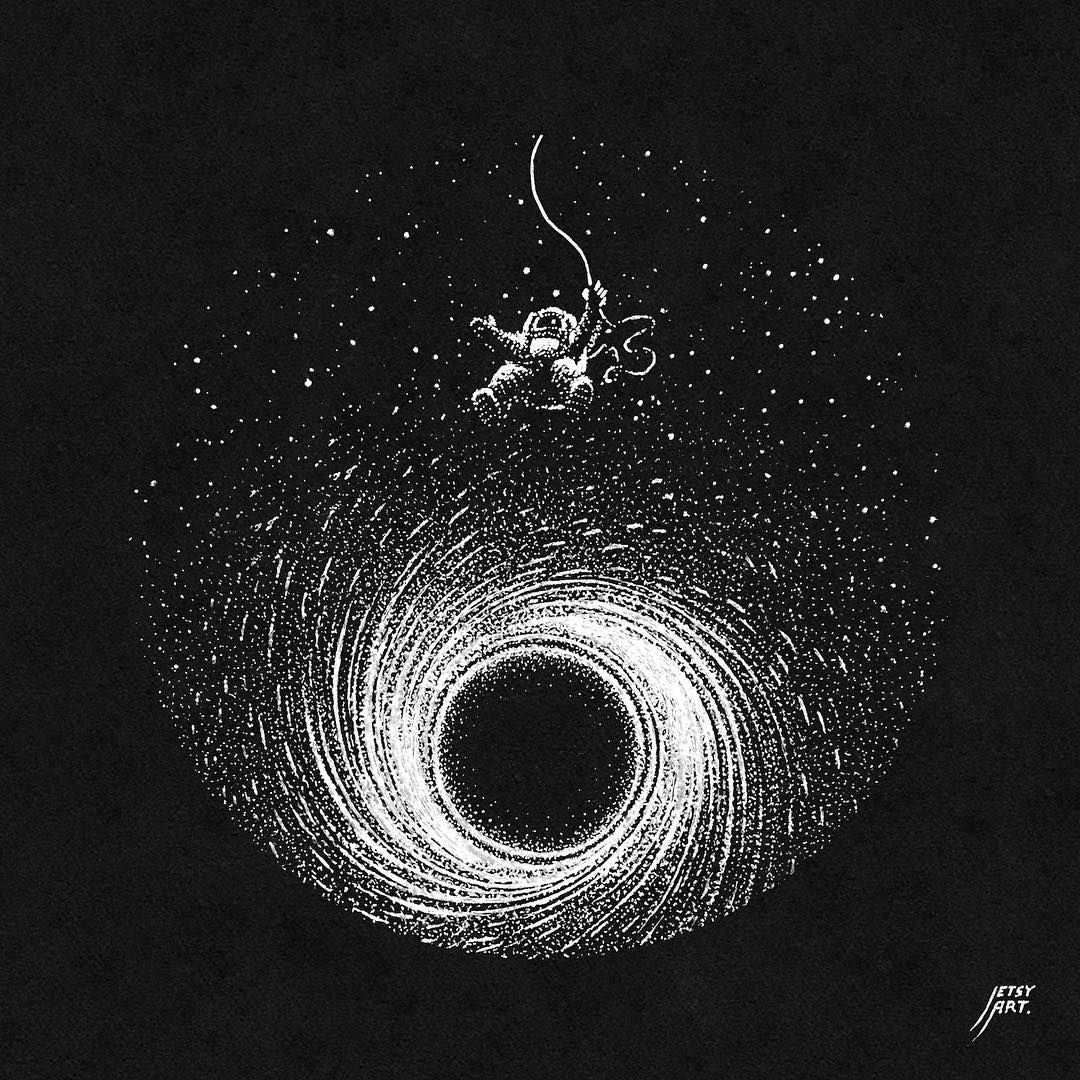
\includegraphics[width=0.8\linewidth]{immagini/blackhole_sketch.jpg}
\end{titlepage}

\tableofcontents
\newpage
\pagestyle{headings}
\section*{Premessa}
Questi appunti sono stati presi seguendo i corsi di  \textit{Introduzione alla relatività generale} e \textit{Gravità e superstringhe 1} tenuti dalla professoressa S. Klemm all'Università degli Studi di Milano.  Ulteriori integrazioni sono state prese dall'analogo corso di introduzione alla relatività generale tenuto dal professore E. Castorina, sempre presso UNIMI. Il testo riporta in bella forma gli appunti presi a lezione, con l'aggiunta di qualche esercizio dato da svolgere e personali integrazioni. In quanto appunti, ciò che è riportato può essere sempre soggetto ad errori. Sono gradite correzioni.

I libri su cui sono stati basati i corsi e da cui sono state prese ulteriori informazioni sono riportati nella bibliografia. Le immagini utilizzate sono in parte prese dai precedenti libri, in parte da ricerche su internet e, soprattutto per le sezioni relative al primo corso di GR, dagli appunti sul corso raccolti da Carlo Mascaretti. Crediti ai rispettivi creatori, ve le ho rubate perché mi piacciono.

I testi maggiormente adottati sono stati \cite{wald}\cite{tong}\cite{tong_cosmo}\cite{hawking}\cite{townsend}\cite{straumann}.
\newpage

\include{capitoli/varietà}
\chapter{Tensori}
I tensori sono oggetti che generalizzano il concetto di vettore e covettore, in quanto come si vedrà sono dotati di proprietà miste.
\begin{definizione}
Siano $V$ e $V^*$ uno spazio vettoriale e il suo duale.
Un \textbf{tensore} del tipo $\binom{r}{s}$ è un'applicazione multilineare:
\begin{equation*}
    T : \underbrace{V^* \times \dots \times V^*}_\text{r volte} \times \underbrace{V \times \dots \times V}_\text{s volte} \rightarrow \mathbb{R}
\end{equation*}
\end{definizione}
Essi sono quindi dei funzionali sullo spazio ottenuto dal prodotto cartesiano tra $V^*$ e $V$ $r$ volte e $s$ volte.
L'insieme dei tensori forma lo spazio vettoriale $V^r_s$


\begin{definizione}
Siano $V, \ W$ due spazi vettoriali su campo $\mathbb{K}$. Il \textbf{prodotto tensoriale} $V \otimes W$ è uno spazio vettoriale che consiste di somme finite
\begin{equation*}
    v_1 \otimes w_1 + v_2 \otimes w_2 + \dots
\end{equation*}
dove valgono le regole:
\begin{itemize}
    \item $(v_1 + v_2)\otimes w = v_1 \otimes w + v_2 \otimes w$
    \item $v\otimes (w_1 + w_2)= v \otimes w_1 + v \otimes w_2$
    \item $(cv)\otimes w= v\otimes (cw) = c ( v \otimes w) $
\end{itemize}
\end{definizione}

\begin{esempio}
Siano $v \in \mathbb{C}^n$ e $w\in \mathbb{C}^m$. Allora
\begin{equation*}
    v \otimes w =
    \begin{pmatrix} a_1 \\ \vdots \\ a_n \end{pmatrix} \otimes     \begin{pmatrix} b_1 \\ \vdots \\ b_m \end{pmatrix} = 
    \begin{pmatrix}
    a_1 \begin{pmatrix}
        b_1 \\
        \vdots\\
        b_m
        \end{pmatrix} \\
    \vdots \\
    a_n \begin{pmatrix}
        b_1 \\
        \vdots\\
        b_m
        \end{pmatrix}
    \end{pmatrix} =
    \begin{pmatrix}
    a_1 b_1 \\ \vdots \\ a_1 b_m \\ \vdots \\ a_n b_1 \\ \vdots \\ a_n b_m
    \end{pmatrix}
\end{equation*}
\end{esempio}


Una base per lo spazio dei tensori $V^r_s$ è data da:
\begin{equation}
    e_{j_1} \otimes \dots \otimes e_{j_r} \otimes \theta^{i_1} \otimes \dots \otimes \theta^{i_s}
\end{equation}
nella quale il generico tensore è descrivibile come:
\begin{equation}
    T = \tensor{T}{^{j_1 \dots j_r}_{i_1 \dots i_s}} e_{j_1} \otimes \dots \otimes e_{j_r} \otimes \theta^{i_1} \otimes \dots \otimes \theta^{i_s}
\end{equation}
Gli elementi $\tensor{T}{^{j_1 \dots j_r}_{i_1 \dots i_s}}$ sono le componenti del tensore nella base scelta. Vediamo ora l'applicazione di un tensore sugli elementi $v \in V, \ u \in V^*$.
Chiamiamo $T(u_1, \dots, u_r, v_1, \dots, v_s) \equiv T$, allora:
\begin{align*}
    T &= \tensor{T}{^{j_1 \dots j_r}_{i_1 \dots i_s}} e_{j_1} \otimes \dots \otimes e_{j_r} \otimes \theta^{i_1} \otimes \dots \otimes \theta^{i_s} (u_1, \dots, u_r, v_1, \dots, v_s) \\
    &= \tensor{T}{^{j_1 \dots j_r}_{i_1 \dots i_s}} e_{j_1}(u_1) \otimes \dots \otimes e_{j_r}(u_r) \otimes \theta^{i_1}(v_1) \otimes \dots \otimes \theta^{i_s}(v_s)\\
    &= \tensor{T}{^{j_1 \dots j_r}_{i_1 \dots i_s}} u_{(1) j_1} \dots u_{(r)j_r} v_{(1)}^{i_1}\dots v_{(s)}^{i_s}
\end{align*}
dove $u_{(r)j_r}$ è la $j_r$-esima componente covariante del covettore $u_r$, mentre $ v_{(s)}^{i_s}$ è la $i_s$-esima componente controvariante del vettore $v_s$.

\begin{definizione}
Chiamiamo \textbf{campo tensoriale} sulla varietà $X$ la funzione:
\begin{equation*}
    T : X \rightarrow (TX)^r_s
\end{equation*}
che associa ad ogni $p \in X$ un tensore definito sullo spazio tangente nel punto. Le sue componenti, al pari delle componenti di un campo vettoriale di cui è la generalizzazione, sono delle funzioni.\footnote{Si richiede anche che il tensore vari con differenziabilità al variare del punto della varietà.} Le componenti del campo tensoriale, come è abbastanza prevedibile, trasformano come un tensore nella trasformazione tra due diverse carte nelle quali sono espresse:
\begin{equation*}
    \tensor{T}{^{j_1\dots j_r}_{i_1\dots i_s}}(x'^1,\dots, x'^n) = \frac{\partial x'^{j_1}}{\partial x^{k_1}} \dots \frac{\partial x'^{j_r}}{\partial x^{k_r}} \frac{\partial x^{l_1}}{\partial x'^{i_1}} \dots \frac{\partial x^{l_s}}{\partial x'^{i_s}} \tensor{T}{^{k_1 \dots k_r}_{l_1\dots l_s}}(x^1,\dots, x^n)
\end{equation*}
\end{definizione}
\section{Cambiamento di base}
Ricordando come trasformano le basi e le componenti, eq. \ref{eq.basetransvett}-\ref{eq.covar}, applichiamo nello sviluppo del tensore:
\begin{align*}
    T &= \tensor{T}{^{j_1 \dots j_r}_{i_1 \dots i_s}} e_{j_1} \otimes \dots \otimes e_{j_r} \otimes \theta^{i_1} \otimes \dots \otimes \theta^{i_s} \\
    &= \tensor{T}{^{j_1 \dots j_r}_{i_1 \dots i_s}} \tensor{a}{_{j_1}^{k_1}} \dots \tensor{a}{_{j_r}^{k_r}} \tensor{(a^{-1})}{^{i_1}_{l_1}} \dots \tensor{(a^{-1})}{^{i_s}_{l_s}} e'_{k_1} \otimes \dots \otimes e'_{k_r} \otimes \theta'^{l_1} \otimes \dots \otimes \theta'^{l_s} \\
    &\equiv \tensor{(T')}{^{k_1 \dots k_r} _{l_1 \dots l_s}}  e'_{k_1} \otimes \dots \otimes e'_{k_r} \otimes \theta'^{l_1} \otimes \dots \otimes \theta'^{l_s}
\end{align*}
ovvero un tensore del tipo $\binom{r}{s}$ trasforma $r$-volte in maniera controvariante e $s$-volte in maniera covariante.
\begin{equation*}
    \tensor{(T')}{^{k_1\dots k_r}_{l_1\dots l_s}} = \tensor{T}{^{j_1 \dots j_r}_{i_1 \dots i_s}} \tensor{a}{_{j_1}^{k_1}} \dots \tensor{a}{_{j_r}^{k_r}} \tensor{(a^{-1})}{^{i_1}_{l_1}} \dots \tensor{(a^{-1})}{^{i_s}_{l_s}}
\end{equation*}
\section{P-Forme differenziali}
\begin{definizione}
Una \textbf{p-forma differenziale} è un tensore $T_{i_1 \dots i_p}$ del tipo $\binom{0}{p}$ totalmente antisimmetrico.

Chiamiamo $\Lambda_p V$ lo spazio delle $p$-forme sullo spazio $V$.
\end{definizione}

Rientrano in questa definizione gli elementi dello spazio cotangente, che erano già state chiamate 1-forme differenziali. Questa definizione generalizza quanto visto.
Una funzione $f: X \rightarrow \mathbb{R}$ è una zero forma.

\begin{esempio}
Siano $\xi_1,\xi_2 \in \mathbb{R}^2$, sviluppati secondo
\begin{align*}
    \xi_1 = \xi_{11}e_1 + \xi_{12} e_2 &&   \xi_2 = \xi_{21} e_1 + \xi_{22} e_2
\end{align*}
allora possiamo definire la 2-forma differenziale:
\begin{equation*}
    S(\xi_1,\xi_2)= 
    \begin{vmatrix}
    \xi_{11} & \xi_{12}\\
    \xi_{21} & \xi_{22}
    \end{vmatrix}
\end{equation*}
che fornisce l'area orientata del parallelogramma generato da $\xi_1, \xi_2$.
Può essere generalizzato a $n$ vettori in $\mathbb{R}^n$ per fornire il volume orientato:
\begin{equation*}
    V(\xi_1, \dots,\xi_n)= 
    \begin{vmatrix}
    \xi_{11} & \dots & \xi_{1n}\\
    \vdots & \ddots & \vdots\\
    \xi_{n1} & \dots & \xi_{nn} \\
    \end{vmatrix}
\end{equation*}
Si veda \cite{arnold}.
\end{esempio}

\begin{definizione}
Siano $\phi \in \Lambda_pV$ e $\chi \in \Lambda_q V$ rispettivamente $p$-forma e $q$-forma. Si definisce \textbf{prodotto esterno o wedge}:
\begin{equation*}
    \phi \wedge \chi = \frac{(p+q)!}{p!q!}\mathcal{A}(\phi \otimes \chi)
\end{equation*}
dove $\mathcal{A}$ è l'operatore di antisimmetrizzazione definito:
\begin{equation*}
    (\mathcal{A}T)(v_1,\dots,v_p) = \frac{1}{p!}\sum_{\theta \in S_p} \epsilon_\theta T( v_{\theta(1)}, \dots, v_{\theta(p)})
\end{equation*}
con $\epsilon_\theta$ il segno della permutazione $\theta$ del gruppo $S_p$ di permutazioni di ordine $p$.
\end{definizione}

Il prodotto esterno permette di ottenere una $(p+q)$-forma.
L'insieme delle $p$-forme, per tutti i valori di $p$, dotato del prodotto wedge forma un'algebra chiamata \textbf{algebra esterna o di Grassmann}; questa è però una \textit{algebra graduata}, in quanto non si possono sommare tra loro forme $p$ e $q$ con $p\neq q$ (i gradi sono dati proprio da questa caratterizzazione interna allo spazio di tutte le forme differenziali).

Il prodotto esterno gode delle proprietà:
\begin{itemize}
    \item multilinearità:
    \begin{itemize}
    \item $\phi \wedge \underbrace{( \chi + \psi)}_ \text{tra $q$-forme} = \phi \wedge \chi + \phi \wedge \psi$
    \item $\underbrace{(\phi + \chi )}_\text{tra $p$-forme} \wedge \psi = \phi \wedge \psi + \chi \wedge \psi$
    \item $f(\phi \wedge \chi)=f \phi \wedge \chi+ \phi \wedge f\chi$
    \end{itemize}
   
    \item non sempre commutativo: $\phi \wedge \chi = (-1)^{pq}\chi \wedge \phi $
    
    \item associatività: $(\phi \wedge \chi)\wedge \psi = \phi \wedge ( \chi \wedge \psi)$
\end{itemize}
\begin{esempio}
Siano $\phi$, $\chi$ 1-forme.
\begin{equation*}
    \phi \wedge \chi = 2 \mathcal{A}(\phi \otimes \chi) = 2\frac{1}{2}(\phi \otimes \chi - \chi \otimes \phi) = \phi \otimes \chi - \chi \otimes \phi
\end{equation*}
\end{esempio}
\textbf{N.B:} se dim$V=n$ allora non esistono $p$-forme con $p>n$ in quanto vorrebbe dire che un indice deve apparire due volte e non può essere totalmente antisimmetrico\footnote{migliorare}

Sia la base $\{ \theta^1, \dots, \theta^n\}$ di $V^*$, allora la \textbf{base di $\Lambda_p V$} è data da:
\begin{equation*}
    \{ \theta^{I_1} \wedge \dots \wedge \theta^{I_p} : I_i= 0, \dots, p, I_i < I_{i+1} \}
\end{equation*}
La dimensione dello spazio delle $p$-forme è $\binom{n}{p}$.
\begin{esempio}
Sia $n=4, \ p=2$ allora la base è:
\begin{equation*}
    \{ \theta^1 \wedge \theta^2, \theta^1 \wedge \theta^3, \theta^1 \wedge \theta^4, \theta^2 \wedge \theta^3, \theta^2 \wedge \theta^4, \theta^3 \wedge \theta^4 \}
\end{equation*}
\end{esempio}

\begin{esempio}
Sia $p=3$, allora il tensore ha sviluppo:
\begin{align*}
    \omega &= \omega_{ijk} \theta^i \otimes \theta^j \otimes \theta^k \\
    &= \omega_{[ijk]} \theta^i \otimes \theta^j \otimes \theta^k
\end{align*}
dove nell'ultimo passaggio si è posto sugli indici l'operatore di antisimmetrizzazione.
\begin{equation*}
    \omega = \frac{1}{3!}( \omega_{ijk} + \omega_{kij} + \omega_{jki} - \omega_{ikj} - \omega_{jik} - \omega_{kji} ) \theta^i \otimes \theta^j \otimes \theta^k
\end{equation*}
Distribuendo le somme e sfruttando la saturazione degli indici, si effettuano i cambi di indice portando tutti gli $\omega$ allo stesso $\omega_{ijk}$:
\begin{align*}
    \omega &= \frac{1}{3!}\omega_{ijk}(
       \theta^i \otimes \theta^j   \otimes \theta^k
    +   \theta^j \otimes \theta^k   \otimes \theta^i
    +   \theta^k \otimes \theta^i   \otimes \theta^j + \\
    &
    -   \theta^j \otimes \theta^i   \otimes \theta^k
    -   \theta^i \otimes \theta^k   \otimes \theta^j
    -   \theta^k \otimes \theta^j   \otimes \theta^i) \\
    &= \frac{1}{3!} \omega_{ijk} \theta^i \wedge \theta^j \wedge \theta^k
\end{align*}
\end{esempio}

Vale \textbf{in generale}:
\begin{equation*}
    \omega = \frac{1}{p!}\omega_{i_1 \dots i_p} \theta^{i_1} \wedge \dots \wedge \theta^{i_p}
\end{equation*}

\begin{definizione}
Sia $\phi \in \Lambda_p V$ espressa nello sviluppo: $\phi = \frac{1}{p!}\phi_{i_1 \dots i_p} dx^{i_1} \wedge \dots \wedge dx^{i_p}$. La \textbf{derivata esterna} di una $p$-forma differenziale è definita come l'unica applicazione $\Lambda_p V \rightarrow \Lambda_{p+1}V$ che soddisfa:
\begin{itemize}
    \item $d(\phi + \chi) = d\phi + d\chi$
    
    \item $d(\phi \wedge \chi)=d\phi \wedge \chi + (-1)^p\phi \wedge d\chi$
    
    \item $dd\phi (:= d^2\phi) = 0$
    
    \item $df = \partial_i f dx^i$ dove $f$ è funzione (0-forma)
\end{itemize}
\end{definizione}
La derivata esterna estende il concetto di differenziale di una funzione a forme differenziali.

Possiamo determinare la formula generale per la derivata esterna $d\phi:$
\begin{align*}
    d\phi &= d(\frac{1}{p!}\phi_{i_1 \dots i_p} dx^{i_1} \wedge \dots \wedge dx^{i_p}) \\
    &= \frac{1}{p!} d\phi_{i_1 \dots i_p} \wedge dx^{i_1} \wedge \dots \wedge dx^{i_p} + \frac{1}{p!}\phi_{i_1 \dots i_p} d(dx^{i_1} \wedge \dots \wedge dx^{i_p})
\end{align*}
    Si può dimostrare usando la seconda proprietà che il termine $d(dx^{i_1} \wedge \dots \wedge dx^{i_p})=0$ e pertanto:
\begin{equation*}
    d\phi = \frac{1}{p!} d\phi_{i_1 \dots i_p} \wedge dx^{i_1} \wedge \dots \wedge dx^{i_p}
\end{equation*}
    A indici $i_1 \dots i_p$ fissati allora $\phi_{i_1 \dots i_p}(x^1, \dots , x^n)$ sono funzioni, cioè è una 0-forma:
\begin{equation}
    d\phi = \frac{1}{p!}\partial_i \phi_{i_1 \dots i_p} dx^i \wedge dx^{i_1} \wedge \dots \wedge dx^{i_p}
    \label{eq.derivesterna}
\end{equation}
è la formula della derivata esterna di una $p$-forma differenziale. Si usa anche la notazione $\phi_{i_1 \dots i_p, i} \equiv \partial_i \phi_{i_1 \dots i_p}$.



\section{Varietà riemanniane e pseudo-riemanniane, tensore metrico}
\begin{definizione}
Sia una varietà differenziabile $X$ dotata di un campo tensoriale $g$ di tipo $\binom{0}{2}$ tale che:
\begin{itemize}
    \item $g$ è simmetrico: $g_{ij} = g_{ji}$
    \item $\forall x \in X$ la forma bilineare $g$ è non degenere
    \begin{equation*}
        g_x(v, w) = 0 \ \forall v \in T_xX \implies w= 0
    \end{equation*}
\end{itemize}
Se $g_x(v,v) > 0 \ \forall v \in T_xX$ la varietà è detta \textbf{riemanniana} (propria), altrimenti si parla di varietà \textbf{pseudo-riemanniana} (impropria).
\end{definizione}
Il campo tensoriale $g$ è chiamato \textbf{tensore metrico}. Nel caso di varietà riemanniane permette di definire le nozioni di distanza, lunghezza, curve geodetiche etc. tramite la definizione di un prodotto scalare definito positivo sullo spazio tangente.
\begin{align*}
    (v | w) = g_x(v,w) &&  \forall v, w  \in T_xX\\
    \| v \| = \sqrt{g_x(v,v)} &&  \forall v \in T_xX
\end{align*}
Se la varietà è pseudo-riemanniana, il prodotto scalare non è definito positivo e ci possono essere vettori con lunghezza negativa.
\begin{esempio}
Sia $\gamma(t) : [a,b] \rightarrow X$ una curva differenziabile sulla varietà riemanniana $X$.
La lunghezza della curva è definita da:
\begin{equation*}
    L(\gamma) = \int_a^b\|\gamma ' (t) \|dt
\end{equation*}
\end{esempio}

Sia $\{\theta^i\}$ campo di vettori covarianti di base, allora scriviamo
\begin{align*}
    g &= g_{ij} \theta^i \otimes \theta^j = \frac{1}{2} g_{ij} \theta^i \otimes \theta^j + \frac{1}{2} g_{ij} \theta^i \otimes \theta^j\\
    &= \frac{1}{2} g_{ij} \theta^i \otimes \theta^j + \frac{1}{2} g_{ji} \theta^j \otimes \theta^i = \frac{1}{2} g_{ij}( \theta^i \otimes \theta^j + \theta^j \otimes \theta^i) \\
    &= g_{ij} \theta^i \theta^j
\end{align*}
dove per l'ultimo termine è stata usata una notazione che alleggerisce la simmetrizzazione detta anche prodotto simmetrizzato. Si scrive anche, nel caso di base naturale:
\begin{equation*}
    g \equiv ds^2 = g_{ij}dx^idx^j
\end{equation*}

Sia $\{e_i\}$ la base duale di $\{\theta^i\}$:
\begin{equation*}
    g_x(v,w) = g_x(v^i e_i,w^j e_j) = v^i w^j g_x(e_i, e_j) = g_{ij} v^i w^j \implies g_x(e_i, e_j)=g_{ij}
\end{equation*}
in tal modo si possono ottenere gli elementi di matrice del tensore $g$.

\subsection{Abbassamento e alzamento indici}
Mostriamo come il tensore $g$ stabilisca un isomorfismo tra $T_x$ e $T_x^*$. Sia $u \in T_x$ allora l'applicazione $g_x(u,\cdot): T_x \rightarrow \mathbb{R}$, dove è lasciato aperto il secondo termine della forma bilineare, è un funzionale su $T_x$, ovvero un elemento di $T_x^*$.
\begin{align*}
    g_x(u,\cdot) : T_x  &\rightarrow \mathbb{R} \\
                v &\mapsto g_x(u,v)
\end{align*}
Chiamiamo pertanto \textbf{isomorfismo canonico} la mappa:
\begin{align*}
    &T_x \rightarrow T_x^* \\
    &u \mapsto g_x(u,\cdot)= u^*
\end{align*}
che per componenti risulta:
\begin{equation*}
    g_x(u,v)=g_{ij} u^iv^j \implies u^*_j = g_{ij}u^i
\end{equation*}
Da qui in poi ometteremo l'indice * e manterremo la distinzione tra vettore e covettore basandoci sull'indice alto o basso. Tramite l'uso della metrica sappiamo dunque come passare da componenti covarianti a controvarianti:
\begin{align*}
    u_i=g_{ij}u^j && u^i=g^{ij}u_j
\end{align*}
La matrice di elementi $g^{ij}$ è l'inversa di $g_{ij}$. Generalizzando ai tensori, cioè sfruttando l'isomorfismo canonico tra $\otimes^pT_x$ e $\otimes^pT_x^*$:
\begin{equation*}
    T_{i_1\dots i_p} = g_{i_1 j_1} \dots g_{i_p j_p} T^{j_1 \dots j_p}
\end{equation*}
L'isomorfismo può essere usato per alzare o abbassare solo alcuni indici, ad esempio:
\begin{equation*}
    T^i_j= g_{jk}T^{ki}
\end{equation*}

\subsection{Ortonormalità, segnatura}
\begin{definizione}
Chiamiamo \textbf{forma quadratica} associata a $g$, l'applicazione
\begin{align*}
    T_xX & \rightarrow \mathbb{R} \\
    v &\mapsto g_x(v, v)
\end{align*}
\end{definizione}

Con la metrica introdotta è possibile quindi definire il concetto di base ortonormale, cioè tale che
\begin{align*}
    g(v_i,v_j) &= 0 \ \ \text{ Se $i\neq j$} \\
    g(v_i,v_i) &= \pm 1 
\end{align*}
La scelta delle possibili basi ortonormali è arbitraria, non lo è però il numero di elementi che risulta $g(v_i,v_i)=1$ e $g(v_j,v_j)=-1$, in quanto dipende dal numero di autovalori positivi e negativi della matrice rappresentativa di $g$: poiché la forma bilineare è simmetrica, la sua matrice rappresentativa ammette base di autovettori ortonormali con autovalori reali; con questa base, in particolare la matrice ortogonale con colonne gli autovettori, è possibile diagonalizzare la rappresentativa di $g$ e quindi ridurre in forma canonica la forma quadratica. Possiamo in particolare applicare il teorema di Sylvester (con $V=T_x X$):
\begin{teorema}[di Sylvester]
Sia $g: V\times V \rightarrow \mathbb{R} $ simmetrica ($n=dimV$) allora $\exists! k \in \mathbb{N}$ e $\exists C$ base di $V$ tale che la matrice che rappresenta $g$ può essere scritta nella forma a blocchi:
\begin{equation*}
    \begin{pmatrix}
    -I_{k} & 0 & 0 \\
    0 & I_{n-k} & 0 \\
    0 & 0 & 0
    \end{pmatrix}
\end{equation*}
ovvero $g_{ij}v^iv^j= - \sum_{j=0}^{k}(v^i)^2 + \sum_{j=k+1}^{n-k}(v^j)^2$
\end{teorema}
\begin{definizione}
Chiamiamo \textbf{segnatura} di una forma quadratica la coppia $(k, n-k)$, cioè il numero di autovalori negativi e positivi.
\end{definizione}
Chiamiamo $k$ l'indice della forma quadratica. In particolare distinguiamo
\begin{itemize}
    \item $k=0$: varietà Riemanniana propria
    
    Il tensore metrico è definito positivo. L'ortonormalizzazione è ottenuta con $(e_i|e_j)= \delta_{ij}$.
    \item $k=1$: varietà Lorentziana
    
    Il tensore metrico non è definito positivo e ha un autovalore negativo; viene chiamato tensore lorentziano. L'ortonormalizzazione è ottenuta con $(e_i|e_j)=\eta_{ij}$. Lo spaziotempo di Minkowski è l'esempio più classico con segnatura $(-+++)$ e $\eta_{ij}=diag(-1,1,1,1)$.
\end{itemize}

\subsection{Elemento di volume e integrazione sulla varietà}\label{para.volume}
\begin{definizione}
Una \textbf{forma di volume o orientazione} della varietà $V$ di dimensione $n$ è una forma differenziale $v$ mai nulla:
\begin{equation*}
    v = v(x)dx^1\wedge \dots \wedge dx^n
\end{equation*}
dove $v(x)\neq 0$ in ogni punto della varietà. Se tale forma esiste ovunque sulla varietà, $V$ è detta \textbf{orientabile}.
\end{definizione}

\begin{definizione}
L'orientazione è detta \textbf{destrorsa} se $v(x) > 0$ in qualsiasi punto della varietà. Se $v(x) < 0 $ in qualsiasi punto, allora è detta \textbf{sinistrorsa}.
\end{definizione}

Le forme di volume dipendono nella loro scrittura dal sistema di coordinate scelto ed in particolare devono mantenere la loro natura destrorsa/sinistrorsa nelle regioni dove due set di coordinate si sovrappongono. Quindi:
\begin{align*}
    v &= v(x) \frac{\partial x^1}{\partial \Bar{x}^{a_1}} d\Bar{x}^{a_1} \wedge \dots  \wedge \frac{\partial x^n}{\partial \Bar{x}^{a_n}}d\Bar{x}^{a_n} \\
    &= v(x)det\left( \frac{\partial x^\mu}{\partial \Bar{x}^\nu}\right) d\Bar{x}^1 \wedge \dots \wedge d\Bar{x}^n
\end{align*}
mantiene la stessa orientazione se $det\left( \frac{\partial x^\mu}{\partial \Bar{x}^\nu}\right) > 0$.

Dato quindi un elemento di volume $v$ sulla varietà $V$, si può integrare una qualsiasi funzione $f : V \rightarrow \mathbb{R}$, nella carta $\phi : O \rightarrow U$  e coordinate $x^\mu$ secondo:
\begin{equation*}
    \int_O fv = \int_U dx_1 \dots dx_n f(x) v(x)
\end{equation*}
La forma di volume fornisce pertanto un peso con il quale valutare le differenti parti dell'integrale. Qualora si voglia integrare sulla varietà, la si suddivide nelle carte che la ricoprono e si esegue l'integrazione sulle carte separate.
Dato invece un campo vettoriale $F$, la sua contrazione con la forma differenziale $v$ sarà una $(n-1)$-forma differenziale che scriviamo $F\cdot v$. Questa può essere integrata su una qualsiasi sottovarietà $\mathcal{V}$ compatta e orientabile di dimensione $(n-1)$ per la quale scriveremo:
\begin{equation*}
    \int_\mathcal{V} F^i d\sigma_i =\int_\mathcal{V}F^i n_i d\sigma = \frac{1}{(n-1)!}\int_\mathcal{V} F\cdot v
\end{equation*}
L'elemento $n_\mu$ definisce la forma normale alla superficie orientabile $\mathcal{V}$, mentre $d\sigma$ è l'elemento di volume sulla sottovarietà $\mathcal{V}$. Questo non è unico a meno che la forma normale $n_\mu$ sia normalizzata; Se la forma $n_i$ è normalizzata per mezzo di una metrica $g$ come $n_i n_j g^{ij} = \pm 1$, allora $d\sigma$ è la misura di volume su $\mathcal{V}$ dovuta alla metrica indotta sulla sottovarietà.

Su una varietà lorentziana 4-dimensionale, come quelle con cui avremo a che fare, la metrica permette di definire l'elemento di volume:
\begin{equation*}
    d\tau = \sqrt{-g} d^4x
\end{equation*}
dove qui $g= det(g_{\mu\nu})$ è il determinante (che è negativo).


\chapter{Connessioni lineari}
Fissati due punti $p, q$ su $X$, con la sola struttura di varietà non c'è modo di poter identificare i due vettori tangenti $v_p, v_q$ così da poter dire se uno è \virgolette{uguale} all'altro, essendo elementi di due spazi differenti. Introduciamo quindi il concetto di \textit{trasporto parallelo} di un vettore tangente da $p$ a $q$ lungo una curva, che ci permetta di ottenere tale risultato. A tal fine verrà visto anche il concetto di \textit{curvatura} o torsione che ci permetterà o meno di dire se l'identificazione di $v_p$ in $v_q$ dipenda o meno dalla curva scelta.
\section{Derivata covariante di vettore, trasporto parallelo}
Introduciamo il concetto di derivata direzionale con il quale costruiremo il trasporto parallelo. Questo operatore svolgerà il ruolo di derivata parziale, ma in modo indipendente dalle coordinate scelte. La prima definizione verrà data sui campi vettoriali e sarà in seguito estesa a campi tensoriali.
\begin{definizione}
Chiamiamo \textbf{derivata covariante} o \textbf{connessione} sulla varietà differenziabile $X$ la mappa
\begin{equation*}
    v \mapsto \nabla v
\end{equation*}
che associa il campo vettoriale $v$ ad un campo tensoriale del tipo $\binom{1}{1}$ tale che valgono
\begin{itemize}
    \item linearità: $\nabla (v + w) = \nabla v +  \nabla w$
    \item Leibniz: $\nabla (fv) = df\otimes v + f\nabla v$ dove $f: X \rightarrow \mathbb{R}$ differenziabile
\end{itemize}
\end{definizione}

Per codificare la connessione si fa uso dei \textbf{coefficienti di connessione} o \textit{simboli di Christoffel} definiti sugli elementi della base dello spazio $T_pX$ e il suo duale, dato un punto $p\in X$.
\begin{equation*}
    \nabla e_i = \tensor{\Gamma}{^j_{ki}} \theta^k \otimes e_j
\end{equation*}
In tal modo possiamo ottenere una definizione esplicita della derivata covariante per il generico campo ($v^i$ sono funzioni):
\begin{align*}
    \nabla v &= \nabla (v^i e_i)= dv^i \otimes e_i + v^j\nabla e_j = (dv^i + v^j \tensor{\Gamma}{^i_{kj}}\theta^k )\otimes e_i
\intertext{usando ora la proprietà della derivata esterna sul primo termine poi portando a base generica}
    &=(\partial_k v^i dx^k + v^j \tensor{\Gamma}{^i_{kj}}\theta^k ) \otimes e_i = ( e_k(v^i)\theta^k + v^j \tensor{\Gamma}{^i_{kj}}\theta^k ) \otimes e_i\\
    \nabla v &= ( e_k(v^i) + v^j\tensor{\Gamma}{^i_{kj}}) \theta^k \otimes e_i
\end{align*}

Utilizzeremo la notazione\footnote{Volutamente non è molto differente dalla notazione introdotta in precedenza $v^i_{,k}=\partial_k v^i$ per il motivo che questa introduce i termini correttivi delle $\Gamma$ invece che la sola derivata parziale.} $\tensor{v}{^i_{;k}}= e_k(v^i) + v^j\tensor{\Gamma}{^i_{kj}}$ per scrivere in maniera compatta la componente del campo tensoriale. Possiamo osservare nel caso della base naturale come la componente,  $\partial_k(v^i) + v^j\tensor{\Gamma}{^i_{kj}}$, sia composta dalla derivata parziale lungo la direzione $k$-esima e una correzione determinata dal coefficiente di correzione.
\begin{definizione}
Chiamiamo \textbf{derivata covariante lungo la curva} con tangente il vettore $u$ la quantità:
\begin{equation*}
    \nabla_u v =(\nabla v)(u)
\end{equation*}
\end{definizione}

Poichè $\nabla v$ è un tensore di tipo $\binom{1}{1}$ a cui stiamo dando in ingresso un vettore, il risultato sarà un vettore, infatti:
\begin{align*}
    \nabla_u v &=(\nabla v)(u) = \tensor{v}{^i_{;k}} \theta^k \otimes e_i (u, \cdot ) = \tensor{v}{^i_{;k}} \theta^k(u) \otimes e_i \\
    &= u^k \tensor{v}{^i_{;k}} e_i = u^k( e_k(v^i) + v^j\tensor{\Gamma}{^i_{kj}})e_i = u^k\nabla_{e_k}v
\end{align*}
Nel caso specifico della direzione di un vettore di base ($v= e_k=\delta^i_ke_i$) si ottiene la formula:
\begin{equation}
    \nabla_{e_j}e_i = \tensor{\Gamma}{^m}_{ji}e_m
    \label{eq.covbasee}
\end{equation}
\begin{definizione}
Si dice che il campo vettoriale $v$ è \textbf{trasportato parallelamente} lungo la curva $C(t)$ se $\nabla_{u_i} v= 0$ con $u_i = \frac{dC^i}{dt}$ per ogni punto della curva.
\begin{align*}
    \nabla_{u_i} v = 0 &\iff u^k( e_k(v^i) + v^j\tensor{\Gamma}{^i_{kj}})= 0 \\
     & \iff u^k( \partial_kv^i + v^j\tensor{\Gamma}{^i_{kj}}) = 0
\end{align*}
\end{definizione}

\subsection{Cambiamento di base}
Vediamo sotto le trasformazioni di cambiamento di base, come trasforma la connessione e i coefficienti.
Consideriamo le trasformazioni:
\begin{align*}
    e_i= \tensor{a}{_i^j} e'_j && v^i = \tensor{(a^{-1})}{_j^i}v'^j && \theta^k = \tensor{(a^{-1})}{_l^k}\theta'^l
\end{align*}

Calcoliamo quindi il differenziale:
\begin{align*}
    dv^i &= \tensor{(a^{-1})}{_l^i}dv'^l + v'^l d\tensor{(a^{-1})}{_l^i}\\
    &= \tensor{(a^{-1})}{_l^i}dv'^l+ v'^l e'_h(\tensor{(a^{-1})}{_l^i})\theta'^h
\end{align*}
Avendo sfruttato $dv = \partial_k vdx^k = e_k(v)\theta^k$. Dunque, effettuando già la sostituzione sull'elemento di base dello spazio tangente:
\begin{align*}
    \nabla v &= (dv^i + v^j \tensor{\Gamma}{^i_{kj}}\theta^k)\otimes \tensor{a}{_i^m}e'_m \\
    &= \left[\tensor{(a^{-1})}{_l^i}dv'^l+ v'^l e'_h(\tensor{(a^{-1})}{_l^i})\theta'^h + v'^l\tensor{(a^{-1})}{_l^j}\tensor{\Gamma}{^i_{kj}}\theta'^h\tensor{(a^{-1})}{_h^k}\right] \otimes \tensor{a}{_i^m}e'_m  \\
\intertext{Raccogliendo $\tensor{(a^{-1})}{_l^i}$ e usando $\tensor{(a^{-1})}{_l^i}\tensor{a}{_i^m}=\tensor{\delta}{_l^m}$:}
    &=\left[ dv'^m  + v'^l\left( \tensor{a}{_i^m}e'_h(\tensor{(a^{-1})}{_l^i}) + \tensor{(a^{-1})}{_l^j}\tensor{a}{_i^m}\tensor{\Gamma}{^i_{kj}}\tensor{(a^{-1})}{_h^k}\right) \theta'^h \right]\otimes e'_m \\
    &\equiv (dv'^m + v'^l \tensor{(\Gamma')}{^m_{hl}}\theta'^h )\otimes e'_m
\end{align*}

In questo modo otteniamo come trasformano i coefficienti di connessione:
\begin{equation}
    \tensor{(\Gamma')}{^m_{hl}} = \tensor{a}{_i^m}\tensor{\Gamma}{^i_{kj}}\tensor{(a^{-1})}{_h^k}\tensor{(a^{-1})}{_l^j} + \tensor{a}{_i^m}e'_h(\tensor{(a^{-1})}{_l^i})
    \label{eq.trasform_christoffel}
\end{equation}
I coefficienti di connessione non sono le componenti di un tensore, ma sono composti da un primo termine che trasforma come tale, mentre il secondo termine no in quanto dipende dalla derivata seconda.

I coefficienti di connessione sono volontariamente costruiti per essere non tensoriali, ma tali che la combinazione $\tensor{v}{^i_{;k}}= e_k(v^i) + v^j\tensor{\Gamma}{^i_{kj}}$ trasformi come un tensore; in questo modo viene preservata la trasformazione come tensore della derivata covariante. Inoltre non essendo componenti di un tensore, non si dovrebbe provare ad alzare e abbassare i loro indici.

\section{Derivata covariante di tensore}
Estendiamo la precedente definizioni al più generico campo tensoriale.
\begin{definizione}
Definiamo la \textbf{derivata covariante di un campo tensore} $t$ di tipo $\binom{p}{q}$, il campo tensoriale $\nabla t$ di tipo $\binom{p}{q+1}$ che lungo il vettore $v$ rispetta
\begin{equation*}
    \nabla t (v, v_1, \dots, v_q, w_1, \dots, w_p) = \nabla_v t( v_1, \dots, v_q, w_1, \dots, w_p)
\end{equation*}
e per il quale valgono:
\begin{itemize}
    \item $\nabla_v (f) = v(f) = v^i\partial_i f$ dove $f:X \rightarrow \mathbb{R}$
    \item $\nabla_v (t+s)= \nabla_v t + \nabla_v s$ dove $t,s$ tensori
    \item $\nabla_v(t \otimes s)= \nabla_v t \otimes s + t \otimes \nabla_v s$
    \item $\nabla_v$ commuta con la contrazione: $\nabla_i (\tensor{t}{^j_{jk}}) = \tensor{(\nabla t)}{_i^j_{jk}}$
\end{itemize}
\end{definizione}
Osserviamo che la prima richiesta coincide con l'interpretazione dei campi vettoriali come derivate direzionali su campi scalari $f$.
Poiché abbiamo già calcolato la derivata covariante di un vettore, a completamento vediamo quella di una 1-forma (covettore) $\alpha$. Sappiamo dalla definizione che dovrà essere a sua volta una 1-forma.
Sfruttando l'ultima proprietà, la derivata covariante in direzione $v$ della contrazione $\alpha \otimes u$ (i.e. $\alpha[u]=\alpha_i u^i$) è uguale alla contrazione di $\nabla_v \alpha \otimes u + \alpha \otimes \nabla_v u$ ovvero
\begin{equation*}
    \nabla_v (\alpha[u]) = (\nabla_v \alpha)(u) + \alpha(\nabla_v u) \implies (\nabla_v \alpha)(u) = \nabla_v(\alpha[u]) - \alpha \nabla_v u
\end{equation*}
Dunque prendendo $u= e_i$ si avrà $\nabla_v\alpha (e_i) = (\nabla_v \alpha)_i$:
\begin{equation*}
    (\nabla_v \alpha)_i = \nabla_v (\alpha_i) - \alpha\nabla_v e_i
\end{equation*}
Per l'ultimo termine si sfrutta quanto già noto:
\begin{equation*}
    \nabla_v e_i =\nabla_{v^ke_k} e_i = v^k\nabla_{e_k}e_i = v^k \tensor{\Gamma}{^j_{ki}}e_j
\end{equation*}
Per ottenere:
\begin{align*}
    (\nabla_v \alpha)_i &= v(\alpha_i) - \alpha(v^k \tensor{\Gamma}{^j_{ki}}e_j)
    = v^ke_k(\alpha_i) - v^k \tensor{\Gamma}{^j_{ki}}\alpha(e_j)\\
    &= v^k(e_k(\alpha_i) - \tensor{\Gamma}{^j_{ki}}\alpha_j)
\end{align*}

Pertanto la derivata covariante di una 1-forma $\alpha$ in direzione del vettore tangente $v$ risulta la 1-forma:
\begin{equation*}
    \nabla_v \alpha = (\nabla_v \alpha)_i\theta^i = v^k(e_k(\alpha_i) -\tensor{\Gamma}{^j_{ki}}\alpha_j)\theta^i
\end{equation*}
In direzione generica abbiamo invece un tensore di tipo $\binom{0}{2}$ definito:
\begin{equation*}
    \nabla \alpha = (e_k(\alpha_i) -\tensor{\Gamma}{^j_{ki}}\alpha_j)\theta^k \otimes \theta^i
\end{equation*}
infatti:
\begin{align*}
    \nabla_v \alpha &= \nabla \alpha (v, \cdot ) = (e_k(\alpha_i) -\tensor{\Gamma}{^j_{ki}}\alpha_j)\theta^k \otimes \theta^i (v, \cdot) \\
    &= (e_k(\alpha_i) -\tensor{\Gamma}{^j_{ki}}\alpha_j)\theta^k(v) \otimes \theta^i =v^k(e_k(\alpha_i) -\tensor{\Gamma}{^j_{ki}}\alpha_j)\theta^i
\end{align*}
Osserviamo che la scrittura ha la stessa forma a meno del fatto che si ha ora un covettore invece di un vettore (seguono alcuni indici differenti) e soprattutto il segno meno al posto del più.
Per l'elemento di base si avrà pertanto:
\begin{align}
    \nabla \theta^i = -\tensor{\Gamma}{^i_{kj}}\theta^k \otimes \theta^j \\
    \nabla_{e_j} \theta^i = -\tensor{\Gamma}{^i_{jm}}\theta^m
\end{align}

Abbiamo ora tutti gli elementi per poter determinare le componenti della derivata covariante di un tensore qualsiasi.
\begin{esempio}
Sia un tensore $\binom{1}{2}$, $t=\tensor{t}{^i_{kl}}e_i \otimes \theta^k \otimes \theta^l$, allora:
\begin{align*}
    \nabla_v t &= \nabla_v( \tensor{t}{^i_{kl}} ) e_i \otimes \theta^k \otimes \theta^l + \tensor{t}{^i_{kl}}(\nabla_v e_i \otimes \theta^k \otimes \theta^l + e_i \otimes \nabla_v \theta^k \otimes \theta^l + e_i \otimes \theta^k \otimes \nabla_v \theta^l ) \\
    &= v(\tensor{t}{^i_{kl}}) e_i \otimes \theta^k \otimes \theta^l + \tensor{t}{^i_{kl}}(
    v^j \tensor{\Gamma}{^m_{ji}}e_m \otimes \theta^k \otimes \theta^l -
    v^j \tensor{\Gamma}{^k_{jm}} e_i \otimes \theta^m \otimes \theta^l - 
    v^j \tensor{\Gamma}{^j_{jm}} e_i \otimes \theta^k \otimes \theta^m ) \\
    &=v^j( e_j(\tensor{t}{^i_{kl}} )+ \tensor{\Gamma}{^i_{jm}}\tensor{t}{^m_{kl}} -
    \tensor{\Gamma}{^m_{jk}}\tensor{t}{^i_{ml}} -
    \tensor{\Gamma}{^m_{jl}}\tensor{t}{^i_{km}}) e_i \otimes \theta^k \otimes \theta^l
\end{align*}
otteniamo la regola generale:
\begin{equation*}
    \nabla_j (\tensor{t}{^i_{kl}} )= e_j(\tensor{t}{^i_{kl}} )+ \tensor{\Gamma}{^i_{jm}}\tensor{t}{^m_{kl}} -
    \tensor{\Gamma}{^m_{jk}}\tensor{t}{^i_{ml}} -
    \tensor{\Gamma}{^m_{jl}}\tensor{t}{^i_{km}}
\end{equation*}
dove si ha sulla correzione di $\Gamma$ un segno più per ogni indice alto, un segno meno per l'indice basso. L'indice della direzione è sempre il primo indice basso del coefficiente di connessione e i restanti indici rimangono a completamento delle somme saturate.
\end{esempio}
\subsection{Derivata covariante del prodotto}
La derivata covariante di un prodotto è identica all'usuale formula per della derivazione.
Notiamo per prima cosa:
\begin{equation*}
    \nabla_j \tensor{t}{^i_{kl}} = \tensor{(\nabla t)}{_j^i_{kl}} = \tensor{(\nabla_j t)}{^i_{kl}}
\end{equation*}

Consideriamo il prodotto tra $\binom{1}{1}$ e $\binom{0}{1}$:
\begin{equation*}
    s \otimes t = (\tensor{s}{^i_k}e_i\otimes \theta^k) \otimes t_l\theta^l = \tensor{s}{^i_k}t_l e_i\otimes \theta^k \otimes \theta^l
\end{equation*}
calcolando la derivata in direzione $e_j$ e usando la regola di Leibniz:
\begin{equation*}
    \nabla_j( s\otimes t) = \nabla_j s \otimes t + s \otimes \nabla_j t \implies \tensor{\left( \nabla_j(s\otimes t)\right)}{^i_{kl}} = \tensor{(\nabla_j s)}{^i_k}t_l + \tensor{s}{^i_k}(\nabla_j t)_l
\end{equation*}
ciò implica
\begin{equation*}
    \tensor{\left(\nabla(s\otimes t)\right)}{_j^i_{kl}} =  \tensor{(\nabla s)}{_j^i_k}t_l + \tensor{s}{^i_k}(\nabla t)_{jl}
\end{equation*}
ovvero
\begin{equation*}
    \nabla_j(\tensor{s}{^i_k}t_l) = t_l \nabla_j \tensor{s}{^i_k} + \tensor{s}{^i_k}\nabla_j t_l
\end{equation*}
che è la solita formula di Leibniz nella derivazione.
\section{Connessione metrica}
Su una varietà differenziabile è possibile definire molte derivate covarianti tramite i simboli di Christoffel e in generale nessuna è preferibile rispetto le altri. Si può infatti notare come tutti i calcoli eseguiti fino ad ora erano indipendenti dalla metrica adottata sulla varietà.

La scelta di una metrica $g$ permette una scelta naturale della connessione sulla varietà e in particolar modo impone condizioni sul trasporto parallelo. Fino ad ora la sua definizione ci ha permesso di avere il vettore tangente in un punto $p$ trasportato nello spazio in un punto $q$, senza tuttavia preservare le proprietà metriche del primo. \'E di particolare interesse mantenere queste caratteristiche perché se ad esempio si considera una curva chiusa, il trasporto lungo tutta essa fino al punto di inizio, ci farebbe ottenere un vettore non solo in generale ruotato, ma di lunghezza differente.
\begin{definizione}
Diciamo che \textbf{la connessione è metrica} se il trasporto parallelo lascia invariato il prodotto scalare, cioè siano $u, w$ e $g$ tensore metrico, allora:
\begin{equation*}
    \nabla_v g(u,w) = 0 \ \forall v \textrm{ se } \nabla_v u = \nabla_v w = 0
\end{equation*}
in altre parole, usando la regola di Leibniz:
\begin{equation*}
    (\nabla_v g)(u,w) = g(\nabla_v u, w) + g(u, \nabla_v w) = 0
\end{equation*}
si scrive allora
\begin{align*}
    \nabla g = 0 &\iff \nabla_i g_{jk} = 0 \\
    &\iff e_i(g_{jk}) -
    \tensor{\Gamma}{^m_{ij}} g_{mk} -
    \tensor{\Gamma}{^m_{ik}} g_{jm} = 0
\end{align*}
\end{definizione}
\section{Tensore di torsione, connessione simmetrica}
La condizione che la connessione sia metrica non permette di determinare i coefficienti di connessione; bisogna porre un ulteriore vincolo.
\begin{definizione}
Siano $u,v$ campi vettoriali lisci e $f: X \rightarrow \mathbb{R}$ differenziabile, si definisce \textbf{parentesi di Lie (commutatore)} il campo vettoriale
\begin{equation*}
    [u,v](f) = u(v(f)) - v(u(f))
\end{equation*}
in un punto $p\in X$ fissato.
\end{definizione}
Essendo un campo vettoriale, può ugualmente essere visto come:
\begin{align*}
    [u, v] : X &\rightarrow TX \\
             p &\mapsto [u, v]|_p   
\end{align*}

Calcoliamo esplicitamente:
\begin{align*}
    [u,v] (f) &= u^i\partial_i(v^j\partial_j f) - v^j\partial_j(u^i\partial_i f) \\
    &= u^i(\partial_iv^j\partial_j f + v^j \partial_i\partial_j f ) - v^j(\partial_j u^i \partial_i f + u^i \partial_j \partial_i f) \\
    &= u^i\partial_iv^j\partial_j f - v^j\partial_j u^i \partial_i f \\
    &= (u^j \partial_j v^i -v^j \partial_j u^i) \partial_i f = [u,v]^i \partial_i f
\end{align*}
Si può mostrare che le parentesi di Lie soddisfano l'identità di Jacobi:
\begin{equation*}
    [[v,u],w] + [[u,w],v] + [[w,v],u] = 0
\end{equation*}
Insieme all'antisimmetria e bilinearità, strutturano uno spazio vettoriale ad algebra di Lie.

\begin{definizione}
Sia $\alpha$ una 1-forma e $v, u$ vettori, si definisce il \textbf{tensore della torsione}
\begin{equation*}
    T(\alpha, v, u) = \alpha( \nabla_u v - \nabla_v u - [v,u]) 
\end{equation*}
\end{definizione}
\begin{definizione}
Diciamo che se $T = 0$ cioè $\nabla_u v - \nabla_v u = [v,u]$ la connessione è \textbf{simmetrica}.
\end{definizione}
Affermiamo (senza al momento dimostrarlo) che la condizione $T \neq 0$ non è compatibile con il principio di equivalenza; ci sarebbe la conseguenza che con $T \neq 0$, particelle con spin differente cadano diversamente in un campo gravitazionale e ciò non è osservato.

Calcoliamo le componenti del tensore di torsione.
\begin{align*}
    \tensor{T}{^i_{kl}} &= T( dx^i, \partial_k, \partial_l ) = dx^i ( \nabla_{\partial_k}\partial_l - \nabla_{\partial_l}\partial_k - [\partial_k, \partial_l] ) \\
    &=dx^i( \tensor{\Gamma}{^j_{kl}}\partial_j + \tensor{\Gamma}{^j_{lk}}\partial_j ) \\
    &= \tensor{\Gamma}{^i_{kl}} - \tensor{\Gamma}{^i_{lk}}
\end{align*}
In tal modo è evidente perché viene detto simmetrico quando il tensore è nullo: gli indici bassi dei coefficienti di connessione commutano e i coefficienti sono simmetrici.

Infine osserviamo che la richiesta che la connessione sia senza torsione, si traduce equivalentemente in: sia $f \in \mathcal{F}$ allora:
\begin{equation*}
    \nabla_u \nabla_ v f = \nabla_v \nabla_u f
\end{equation*}
ciò comporta che, facendo uso della prima proprietà della derivata covariante, si può sostituire $\partial \leftrightarrow \nabla$ nel calcolo delle componenti del commutatore e quindi ottenere:
\begin{equation}
    [u,v]^i = u^j\nabla_j v^i - v^j\nabla_ju^i
    \label{eq.commutnabla}
\end{equation}
ma solo se si assume che non ci sia torsione.
\section{Connessione di Levi-Civita}
Mostriamo come, partendo dalle richieste che la connessione sia metrica e simmetrica, sia possibile determinare completamente i coefficienti di connessione.

Partendo dall'ipotesi che la connessione sia metrica, $\nabla g =0$, scriviamo per componenti:
\begin{equation*}
    g_{jk;i}=g_{jk,i} -\tensor{\Gamma}{^m_{ij}} g_{mk} - \tensor{\Gamma}{^m_{ik}} g_{jm} = 0
\end{equation*}
Riscriviamo la stessa equazione permutando gli indici:
\begin{align*}
    g_{ki;j}=g_{ki,j} -\tensor{\Gamma}{^m_{jk}} g_{mi} - \tensor{\Gamma}{^m_{ji}} g_{km} = 0 \\
    g_{ij;k}=g_{ij,k} -\tensor{\Gamma}{^m_{ki}} g_{mj} - \tensor{\Gamma}{^m_{kj}} g_{im} = 0
\end{align*}
Sommiamo alla prima, la seconda e sottraiamone la terza:
\begin{equation*}
    g_{jk,i} -\tensor{\Gamma}{^m_{ij}} g_{mk} - \tensor{\Gamma}{^m_{ik}} g_{jm} + g_{ki,j} -\tensor{\Gamma}{^m_{jk}} g_{mi} - \tensor{\Gamma}{^m_{ji}} g_{km} - g_{ij,k} +\tensor{\Gamma}{^m_{ki}} g_{mj} + \tensor{\Gamma}{^m_{kj}} g_{im} = 0
\end{equation*}
Sfruttiamo la simmetria del tensore metrico e della connessione per eliminare alcuni termini:
\begin{equation*}
    g_{jk,i} + g_{ki,j} - g_{ij,k} -2\tensor{\Gamma}{^m_{ij}} g_{mk} = 0
\end{equation*}
Moltiplicando per la metrica inversa $g^{kl}$ otteniamo che la scrittura della connessione è totalmente determinata dalla metrica, dalla sua inversa e dalle sue derivate.
\begin{definizione}
Chiamiamo una connessione metrica e simmetrica, \textbf{connessione di Levi-Civita}. Essa risulta completamente determinata da
\begin{equation}
   \tensor{\Gamma}{^l_{ij}} = \frac{1}{2}g^{lk}( g_{jk,i} + g_{ki,j} - g_{ij,k} )
\label{eq.connlevicivita}
\end{equation}
\end{definizione}

Risulta utile al fine di esercizi la formula della contrazione della connessione:
\begin{equation}
    \tensor{\Gamma}{^\nu_{\nu\mu}} = \partial_\mu \log\sqrt{|g|}
    \label{eq.traccia_christoffel}
\end{equation}
dove $g$ è il determinante di $g_{\mu\nu}$. Infatti prendendo eq. \ref{eq.connlevicivita} e facendone la traccia:
\begin{align*}
    \tensor{\Gamma}{^\nu_{\nu\mu}} &= \frac{1}{2} g^{\nu\sigma}( g_{\mu\sigma,\nu} + g_{\sigma\nu,\mu} - g_{\nu\mu,\sigma})
    =\frac{1}{2}( g^{\nu\sigma} g_{\mu\sigma,\nu} +g^{\nu\sigma} g_{\sigma\nu,\mu} - g^{\nu\sigma}g_{\nu\mu,\sigma})\\
    \intertext{mandando $\nu\rightarrow\sigma$ e $\sigma\rightarrow\nu$ nel primo termine e usando la simmetria di $g$:}
    &=\frac{1}{2}(g^{\sigma\nu}g_{\mu\nu,\sigma} + g^{\nu\sigma} g_{\sigma\nu,\mu} - g^{\nu\sigma}g_{\nu\mu,\sigma}) \\
    &= \frac{1}{2}g^{\nu\sigma}g_{\sigma\nu,\mu}
\end{align*}
Se si considera l'identità $\Tr(A^{-1}\cdot\partial_\mu A)=\frac{1}{\det A}\partial_\mu A$ dove $A$ è una qualunque matrice non singolare, si può osservare che la traccia del coefficiente è pari a $\frac{1}{2}\Tr(G^{-1}\cdot\partial_\mu G)$, dove $G$ è la matrice del tensore metrico. Pertanto si ottiene:
\begin{equation*}
    \tensor{\Gamma}{^\nu_{\nu\mu}} = \frac{1}{2|g|}\partial_\mu g = \partial_\mu \log\sqrt{|g|}
\end{equation*}

Come conseguenza di tale formula, si ha che la divergenza covariante di un vettore $v$ può essere calcolata tramite:
\begin{equation*}
    \nabla_\mu v^\mu = \frac{1}{\sqrt{|g|}}\partial_\mu(\sqrt{|g|}v^\mu)
\end{equation*}
Infatti è nota $\nabla_\mu v^\nu = \partial_\mu v^\nu + v^\sigma\tensor{\Gamma}{^\nu_{\mu\sigma}}$ che specializzata:
\begin{align*}
    \nabla_\mu v^\mu = \partial_\mu v^\mu + v^\sigma\tensor{\Gamma}{^\mu_{\mu\sigma}} = \partial_\mu v^\mu + v^\sigma\partial_\sigma \log\sqrt{|g|} = \partial_\mu v^\mu + v^\mu \partial_\mu \log\sqrt{|g|}
\end{align*}
D'altra parte
\begin{equation*}
    \frac{1}{\sqrt{|g|}} \partial_\mu (\sqrt{|g|} v^\mu )= \frac{1}{\sqrt{|g|}}\sqrt{|g|}\partial_\mu v^\mu + v^\mu \frac{1}{2|g|}\partial_\mu g = \partial_\mu v^\mu + v^\mu\partial_\mu \log\sqrt{|g|}
\end{equation*}

\subsection{Variazione dei simboli di Christoffel rispetto la metrica}\label{para.variaz_connessione}
I simboli di Christoffel $\Gamma$ non sono dei tensori. Tuttavia sotto variazione della metrica, la quantità variata $\delta \Gamma$ trasforma come tensore in quanto corrisponde alla differenza tra i simboli di Christoffel calcolati con $g_{\mu\nu}$ e con $g_{\mu\nu} + \delta g_{\mu\nu}$. Facendo riferimento a eq. \ref{eq.connlevicivita}, si ottiene nell'eseguire la differenza:
\begin{equation*}
    \delta\tensor{\Gamma}{^\sigma_{\mu\nu}} = \frac{1}{2} g^{\sigma\lambda} (\partial_\nu \delta g_{\lambda \mu} + \partial_\mu \delta g_{\lambda \nu} - \partial_\lambda \delta g_{\mu \nu} )
\end{equation*}
Ora, $\forall p \in \mathcal{M}$ è possibile determinare nell'intorno di $p$ delle coordinate tali che:
\begin{align*}
    g_{\mu\nu}(p) = \nu_{\mu\nu} && g_{\mu\nu,\rho}(p) = 0
\end{align*}
Queste coordinate sono chiamate \textbf{coordinate normali}. Sempre da eq. \ref{eq.connlevicivita} si ottiene che i simboli di connessione sono nulli in questo punto:
\begin{equation*}
    \tensor{\Gamma}{^\sigma_{\mu\nu}} (p) = 0
\end{equation*}
Facendo uso di queste coordinate,  è possibile eseguire $\partial_\lambda g_{\mu\nu} = \nabla_\lambda g_{\mu\nu}$ e pertanto, valutando in $p$:
\begin{equation*}
    \delta\tensor{\Gamma}{^\sigma_{\mu\nu}} = \frac{1}{2} g^{\sigma\lambda} (\nabla_\nu \delta g_{\lambda \mu} + \nabla_\mu \delta g_{\lambda \nu} - \nabla_\lambda \delta g_{\mu \nu} )
\end{equation*}
Il membro di destra è un tensore, in quanto dipende solamente da $\delta g_{\mu\nu}$, quindi il membro a sinistra è anch'esso tensore. Pertanto l'espressione derivata nel sistema di coordinate normali deve valere in tutti i sistemi di coordinate e, data l'arbitrarietà di $p$, deve valere in generale.

\section{Connessione di spin}\label{para.veilbein}
Introduciamo ora una distinzione tra gli indici greci e latini. Con indici latini indicheremo le generiche componenti rispetto una base qualsiasi dello spazio tangente e cotangente (come fatto fino ad adesso). Con indici greci, come usato principalmente in relatività generale, intenderemo invece che le basi dei due spazi sono basi di sistemi di coordinate, quindi basi con proprietà particolari di simmetria per lo spaziotempo. Questo tipo di notazione viene chiamata \textbf{abstract index notation} e fu introdotta da Penrose. 
Gli indici latini pertanto definiscono delle \textit{vere} equazioni tensoriali, indipendenti dalla base scelta e ci ricordano il numero e il tipo di variabili sulle quali agisce il tensore. Le equazioni scritte in indici greci saranno da leggere come equazioni per le componenti; in altre parole $\tensor{T}{^{\mu\nu\rho}_{\sigma\lambda}}$ sarà la componente di una base del tensore  $\tensor{T}{^{abc}_{de}}$ di tipo $\binom{3}{2}$. 
Ciò risulta particolarmente importante quando si discutono le teorie di gauge, come il caso di Chern-Simons, visto che ci sono richieste meno stringenti sulla scelta della base.

In tutti i vari calcoli di relatività generale si è fatto uso delle basi di $T_p M$ e $T_p^*M$ date da:
\begin{align*}
    \hat{e}_{(\mu)} &= \partial_\mu  \\
    \hat{\theta}^{(\mu)} &= dx^\mu
\end{align*}
con $x^\mu$ delle coordinate, quindi con un significato fisico ben preciso. Consideriamo ora una base qualsiasi:
\begin{equation*}
\begin{array}{cc}
     \hat{e}_{(a)} & a = 0, 1, \dots, d-1
\end{array}
\end{equation*}
e scegliamo questa ortonormale:
\begin{equation*}
    g(\hat{e}_{(a)}, \hat{e}_{(b)} ) = \eta_{ab}
\end{equation*}
con $\eta_{ab}$ la metrica di Minkowski di dimensione $d$. In dimensione $4$ questa base verrà chiamata \virgolette{tetrade}, in dimensione 3 \virgolette{triade} e così via\footnote{Viene fatto notare che la tetrade viene chiamata in tedesco \virgolette{vierbein} ovvero \virgolette{4 gambe}, mentre il caso generale viene detto \virgolette{vielbein} ovvero \virgolette{molte gambe}}.

Sviluppiamo una base nell'altra, tramite un'opportuna matrice invertibile di trasformazione:
\begin{equation}
    \hat{e}_{(a)} = \tensor{e}{^\mu_a}\hat{e}_{(\mu)}
    \label{eq.trasform_base_tang_indici_abstr}
\end{equation}
con $\tensor{e}{^\mu_b}\tensor{e}{^a_\mu} = \tensor{\delta}{^a_b}$ e $\tensor{e}{^\mu_a}\tensor{e}{^a_\nu} = \tensor{\delta}{^\mu_\nu}$.
La condizione di ortonormalità diventa:
\begin{equation*}
       g(\hat{e}_{(a)}, \hat{e}_{(b)})=  \tensor{e}{^\mu_a}\tensor{e}{^\nu_b} g( \hat{e}_{(\mu)}, \hat{e}_{(\nu)}) = g_{\mu\nu}\tensor{e}{^\mu_a}\tensor{e}{^\nu_b} = \eta_{ab}
\end{equation*}
dunque:
\begin{equation*}
    g_{\mu\nu} = \tensor{e}{^a_\mu} \tensor{e}{^b_\nu} \eta_{ab}
\end{equation*}
Similmente nello spazio cotangente, data la base ortonormale scelta come:
\begin{equation*}
    \hat{\theta}^{(a)}(\hat{e}_{(b)}) = \tensor{\delta}{^a_b}
\end{equation*}
allora:
\begin{equation*}
    \hat{\theta}^{(a)}(\tensor{e}{^\mu_b}\hat{e}_{(\mu)}) = \tensor{e}{^\mu_b} \hat{\theta}^{(a)}(\hat{e}_{(\mu)}) = \tensor{\delta}{^a_b} 
\end{equation*}
moltiplicando per $\tensor{e}{^b_\nu}$:
\begin{equation*}
    \tensor{\delta}{^\mu_\nu}\hat{\theta}^{(a)}(\hat{e}_{(\mu)}) = \tensor{e}{^a_\nu} \implies \hat{\theta}^{(a)}(\hat{e}_{(\nu)}) = \tensor{e}{^a_\nu}
\end{equation*}
Se scriviamo $\hat{\theta}^{(a)} = \tensor{f}{^a_\mu}dx^\mu$ come trasformazione per la base cotangente, si ottiene sostituendo nella precedente:
\begin{equation*}
    \tensor{f}{^a_\mu} dx^\mu( \hat{e}_{(\nu)}) = \tensor{f}{^a_\nu} = \tensor{e}{^a_\nu}
\end{equation*}
così otteniamo che la trasformazione per il duale è:
\begin{equation}
    \hat{\theta}^{(\mu)} = \tensor{e}{^\mu_a}\hat{\theta}^{(a)} \iff \hat{\theta}^{(a)} = \tensor{e}{^a_\mu} \hat{\theta}^{(\mu)}
    \label{eq.trasform_base_cotang_indici_abstr}
\end{equation}
\begin{esempio}
Data una metrica, ad esempio la statica sfericamente simmetrica:
\begin{equation*}
    ds^2 = - V(r)dt^2 + \frac{dr^2}{V(r)} + r^2(d\theta^2 + \sin^2\theta d\phi^2)
\end{equation*}
Il formalismo risulta particolarmente utile perché si ottengono direttamente:
\begin{align*}
    \hat{\theta}^{(0)} &= \sqrt{V(r)} dt \qquad
    \hat{\theta}^{(1)} = \frac{dr}{\sqrt{V(r)}} \\
    \hat{\theta}^{(2)} &= rd\theta \qquad
    \hat{\theta}^{(3)} = r\sin\theta d\phi
\end{align*}
e quindi si possono riconoscere velocemente:
\begin{align*}
    \tensor{e}{^0_t} &= \sqrt{V(r)} \qquad
    \tensor{e}{^1_r} = \frac{1}{\sqrt{V(r)}} \\
    \tensor{e}{^2_\theta} &= r \qquad
    \tensor{e}{^3_\phi} = r\sin\theta
\end{align*}
con tutti gli altri elementi nulli.
\end{esempio}

Le basi $\hat{e}_{(a)}$ possono essere cambiate indipendentemente dalle coordinate:
\begin{equation*}
    \hat{e}_{(a)}\mapsto \hat{e}_{(a)}' = \tensor{\Lambda}{_a^b}(x)\hat{e}_{(b)}
\end{equation*}
dove $\tensor{\Lambda}{_a^b}(x)$ dipendono dal punto e quindi sono trasformazioni locali. Se imponiamo che sia mantenuta l'ortonormalità:
\begin{align*}
    \eta_{ab} &= g(\hat{e}_{(a)}, \hat{e}_{(b)}) = g(\tensor{\Lambda}{_a^c}(x)\hat{e}_{(c)}, \tensor{\Lambda}{_b^d}(x)\hat{e}_{(d)}) \\
    &= \tensor{\Lambda}{_a^c}(x) \tensor{\Lambda}{_b^d}(x) g(\hat{e}_{(c)}, \hat{e}_{(d)}) = \tensor{\Lambda}{_a^c}(x)\tensor{\Lambda}{_b^d}(x)\eta_{cd}
\end{align*}
Si trova che le trasformazioni $\Lambda$ devono lasciare in ogni punto la metrica di Minkowski invariante. Sono pertanto delle \textbf{trasformazioni di Lorentz locali}.

In questa maniera si introduce in relatività generale, oltre alla possibilità di cambiare le coordinate tramite diffeomorfismi, la libertà di eseguire trasformazioni di Lorentz locali. Un oggetto può quindi possedere entrambi gli indici come ad esempio il tensore:
\begin{equation*}
    \tensor{(T')}{^{a\mu}_{b\nu}} = \tensor{(\Lambda^{-1})}{_c^a}\frac{\partial x'^\mu}{\partial x^\lambda}\tensor{\Lambda}{_b^d}\frac{\partial x^\rho}{\partial x'^\nu}\tensor{T}{^{c\lambda}_{d\rho}}
\end{equation*}
per il quale gli indici greci trasformano col jacobiano/jacobiano inverso della trasformazione delle coordinate mentre quelli latini trasformano con le Lorentz locali.

La derivata covariante per indici greci è la solita nota: derivata parziale corretta affinché trasformi come tensore con i simboli di Christoffel di eq. \ref{eq.connlevicivita}. In una base arbitraria si può fare la stessa procedura introducendo però i simboli della \textbf{connessione di spin}\footnote{Il nome è dovuto al fatto che si possono eseguire derivate covariante di spinori in spazitempo curvi. I fermioni sono nella rappresentazione 4-dimensionale del gruppo di Lorentz con quantizzazione data dall'algebra di Clifford $\{ \gamma^\mu, \gamma^\nu\} = 2\eta^{\mu\nu}$. Il formalismo permette di generalizzarla in $\{\gamma^\mu, \gamma^\nu\} = 2g^{\mu\nu}$ con le $\gamma$ nello spazio curvo date da $\gamma^\mu(x) = \gamma^a \tensor{e}{^\mu_a}$.} $\tensor{\omega}{_\mu^a_b}$:
\begin{equation}
    \nabla_\mu \tensor{X}{^a_b} = \partial_\mu \tensor{X}{^a_b} + \tensor{\omega}{_\mu^a_c}\tensor{X}{^c_b} - \tensor{\omega}{_\mu^c_b}\tensor{X}{^a_c}
    \label{eq.deriv_covar_indici_latini}
\end{equation}
con correzione di segno negativo per indice basso e segno positivo per l'indice alto. In questa maniera questo oggetto trasforma correttamente sia sotto diffeomorfismi sia sotto trasformazioni di Lorentz locali.

Possiamo determinare una relazione tra i coefficienti della connessione di spin e di Levi-Civita. Consideriamo un vettore $X^\mu$ e:
\begin{equation*}
    \nabla X = (\nabla_\mu X^\nu) dx^\mu \otimes \partial_\nu = (\partial_\mu X^\nu + \tensor{\Gamma}{^\nu_{\mu\lambda}}X^\lambda)dx^\mu \otimes \partial_\nu
\end{equation*}
D'altra parte vale:
\begin{align*}
    \nabla X &= (\nabla_\mu X^a) dx^\mu \otimes \hat{e}_{(a)} = (\partial_\mu X^a + \tensor{\omega}{_\mu^a_b}X^b) dx^\mu \otimes \hat{e}_{(a)} \\
    &= \left[\partial_\mu( \tensor{e}{^a_\nu}X^\nu) + \tensor{\omega}{_\mu^a_b}\tensor{e}{^b_\lambda}X^\lambda\right] dx^\mu \otimes (\tensor{e}{^\sigma_a}\partial_\sigma) \\
    &= \tensor{e}{^\sigma_a}(\tensor{e}{^a_\nu}\partial_\mu X^\nu  + X^\nu\partial_\mu\tensor{e}{^a_\nu} + \tensor{\omega}{_\mu^a_b}\tensor{e}{^b_\lambda}X^\lambda ) dx^\mu \otimes \partial_\sigma \\
    &= ( \partial_\mu X^\sigma + \tensor{e}{^\sigma_a}X^\nu\partial_\mu \tensor{e}{^a_\nu} + \tensor{e}{^\sigma_a}\tensor{e}{^b_\lambda}\tensor{\omega}{_\mu^a_b} X^\lambda )dx^\mu \otimes \partial_\sigma
\end{align*}
Poiché gli indici $\sigma, \nu$ sono saturati, mandiamo $\sigma \mapsto \nu$ in tutti e tre i termini, mentre nel secondo $\nu \mapsto \lambda$:
\begin{align*}
    \nabla X &= ( \partial_\mu X^\nu + \tensor{e}{^\nu_a}X^\lambda\partial_\mu \tensor{e}{^a_\lambda} + \tensor{e}{^\nu_a}\tensor{e}{^b_\lambda}\tensor{\omega}{_\mu^a_b} X^\lambda )dx^\mu \otimes \partial_\nu \\
    &\equiv (\partial_\mu X^\nu + \tensor{\Gamma}{^\nu_{\mu\lambda}}X^\lambda)dx^\mu \otimes \partial_\nu
\end{align*}
e quindi:
\begin{equation*}
    \tensor{\Gamma}{^\nu_{\mu\lambda}} = \tensor{e}{^\nu_a}\partial_\mu\tensor{e}{^a_\lambda} + \tensor{e}{^\nu_a}\tensor{e}{^b_\lambda}\tensor{\omega}{_\mu^a_b}
\end{equation*}
ovvero:
\begin{equation}
    \tensor{\omega}{_\mu^a_b} = \tensor{e}{^a_\nu}\tensor{e}{^\lambda_b}\tensor{\Gamma}{^\nu_{\mu\lambda}} - \tensor{e}{^\lambda_b}\partial_\mu \tensor{e}{^a_\lambda}
    \label{eq.legame_conn_spin_levicivita}
\end{equation}
Si può notare che questa è equivalente a (moltiplica  a sinistra da entrambi i lati per $\tensor{e}{^b_\rho}$):
\begin{equation}
    \nabla_\mu \tensor{e}{^a_\rho} = 0
\end{equation}
cioè che la tetrade è covariantemente costante.

Vediamo come il fatto che la metrica sia covariantemente costante si ripercuota sugli indici latini. Poiché scegliamo nella triade/tetrade una base ortonormale:
\begin{equation*}
    \nabla g = 0 \iff \nabla \eta = 0
\end{equation*}
Esplicitamente:
\begin{equation*}
    \nabla_\mu \eta_{ab} = \partial_\mu \eta_{ab} - \tensor{\omega}{_\mu^c_a}\eta_{cb}- \tensor{\omega}{_\mu^c_b}\eta_{ac} = 0
    \iff \omega_{\mu a b} = - \omega_{\mu ba}
\end{equation*}
La connessione di spin è antisimmetrica negli indici latini, che si abbassano/alzano con Minkowski.
\chapter{Geodetiche}
Il concetto di geodetica viene introdotto dal problema variazionale di determinare la curva più breve (o lunga, in ogni caso estremale) tra due punti della varietà. Risulterà abbastanza evidente, come già intuibile, che quanto verrà visto non sarà differente da quanto già affrontato in meccanica classica con l'introduzione dell'Azione e del principio di Minima Azione; basterà pensare alla lunghezza della curva come azione e identificare correttamente la lagrangiana del sistema. Anzi non risulterebbe nemmeno necessario effettuare ulteriori calcoli noto che le equazioni di Eulero-Lagrange forniscono proprio tale curva. Tuttavia procederemo con il calcolo completo per evidenziare delle sottigliezze.

\section{Equazione delle geodetiche}\label{para.geodetiche}
Consideriamo una varietà riemanniana propria $X$, la generalizzazione al caso lorentziano risulterà poi banale per via di un segno. Sia $C(t)$ tale che $C(t_0)=p$, $C(t_1)= q$ dati $p, q \in X$ fissati. La lunghezza della curva è descritta dalla metrica come\footnote{In particolare questo tipo di lagrangiana descrive una particella (massiva, basta aggiungere un fattore $-m$ all'inizio) in moto libero. L'equazione delle geodetiche descriverà successivamente il moto libero nello spaziotempo.}:
\begin{equation*}
    l = \int_{C}ds = \int_{C} \sqrt{ds^2} = \int_{C}\sqrt{g_{ij}dx^idx^j}
\end{equation*}
Siccome la curva è descritta da una parametrizzazione\footnote{La lunghezza è invariante dalla parametrizzazione. Definendo una riparametrizzazione $t\rightarrow\lambda(t)$ si avrà $dt= \frac{dt}{d\lambda}d\lambda$ e quindi $$\sqrt{g_{ij}\frac{dx^i}{dt}\frac{dx^j}{dt}}dt \rightarrow \sqrt{g_{ij}\frac{dx^i}{d\lambda}\frac{d\lambda}{dt}\frac{dx^j}{d\lambda}\frac{d\lambda}{dt}}\frac{dt}{d\lambda}d\lambda$$ che lascia invariato l'integrando.}, si ha:
\begin{equation*}
    l = \int_{t_0}^{t_1}\sqrt{g_{ij}\frac{dx^i}{dt}\frac{dx^j}{dt}}dt
\end{equation*}

Effettuiamo la variazione
\begin{align*}
    \delta l &= \int_{t_0}^{t_1} \frac{1}{2} \left( g_{ij}\frac{dx^i}{dt}\frac{dx^j}{dt} \right)^{-1/2}\left[ \delta g_{ij}\frac{dx^i}{dt}\frac{dx^j}{dt} + g_{ij}\frac{d\delta x^i}{dt}\frac{dx^j}{dt} + g_{ij}\frac{d\delta x^j}{dt}\frac{dx^i}{dt} \right]dt \\
    & = \int_{t_0}^{t_1} \frac{1}{2} \left( g_{ij}\frac{dx^i}{dt}\frac{dx^j}{dt} \right)^{-1/2}\left[ \delta g_{ij}\frac{dx^i}{dt}\frac{dx^j}{dt} + 2g_{ij}\frac{d\delta x^i}{dt}\frac{dx^j}{dt} \right]dt\\
\intertext{A questo punto possiamo fare la scelta, equivalente ad una scelta di gauge, di porre il termine sotto radice pari all'unità, che corrisponde a parametrizzare secondo coordinata curvilinea (ovvero il tempo proprio $\tau$). Questo passaggio può essere fatto solo dopo aver variato $l$.}
    &= \int_{t_0}^{t_1} \left[ \frac{1}{2}\delta g_{ij}\frac{dx^i}{dt}\frac{dx^j}{dt} + g_{ij}\frac{d\delta x^i}{dt}\frac{dx^j}{dt} \right]dt \\
\intertext{Applicando la \emph{chain rule} a $\delta g_{ij}$ nonché integrando per parti il secondo termine e considerando che il termine di bordo $\delta x^k |^q_p$ si annulla:}    
    &=\int_{t_0}^{t_1} \left[ \frac{1}{2}g_{ij,k}\delta x^k\frac{dx^i}{dt}\frac{dx^j}{dt} - \delta x^k \frac{d}{dt}\left(g_{kj}\frac{dx^j}{dt} \right) \right]dt  \\ &= \int_{t_0}^{t_1} \left[ \frac{1}{2}g_{ij,k}\frac{dx^i}{dt}\frac{dx^j}{dt} - \frac{d}{dt}\left(g_{kj}\frac{dx^j}{dt} \right) \right]\delta x^kdt\equiv 0
\end{align*}
Otteniamo l'equivalente equazione di Eulero-Lagrange:
\begin{equation*}
    \frac{1}{2}g_{ij,k}\frac{dx^i}{dt}\frac{dx^j}{dt} - \frac{d}{dt}\left(g_{kj}\frac{dx^j}{dt} \right) = 0
\end{equation*}
Riscriviamola con l'intenzione di far comparire i coefficienti di connessione. Svolgiamo la derivata del prodotto osservando che $g$ è funzione del punto sulla varietà, a sua volta dipendente dal parametro $t$.
\begin{align*}
    \frac{d}{dt}g_{kj}= g_{kj,i}\frac{dx^i}{dt} \longrightarrow     \frac{1}{2}g_{ij,k}\frac{dx^i}{dt}\frac{dx^j}{dt} - g_{kj,i}\frac{dx^i}{dt}\frac{dx^j}{dt} - g_{kj}\frac{d^2 x^j}{dt^2} = 0
\end{align*}
Dividendo il secondo termine in due somme e rinominando indici:
\begin{align*}
    &g_{kj,i}\frac{dx^i}{dt}\frac{dx^j}{dt} = \frac{1}{2}g_{kj,i}\frac{dx^i}{dt}\frac{dx^j}{dt} + \frac{1}{2}g_{ki,j}\frac{dx^j}{dt}\frac{dx^i}{dt} \\
    &\longrightarrow g_{kj}\frac{d^2x^j}{dt^2}= \frac{1}{2}\left(  g_{ij,k}\frac{dx^i}{dt}\frac{dx^j}{dt} -  g_{kj,i}\frac{dx^i}{dt}\frac{dx^j}{dt} -  g_{ki,j}\frac{dx^j}{dt}\frac{dx^i}{dt} \right)
\end{align*}
Moltiplicando per la metrica inversa $g^{lk}$:
\begin{equation*}
    \frac{d^2 x^l}{dt^2} + \frac{1}{2}g^{lk}( g_{kj,i} + g_{ki,j} - g_{ij,k} ) \frac{dx^i}{dt}\frac{dx^j}{dt} = 0
\end{equation*}
Otteniamo infine, richiamando eq. \ref{eq.connlevicivita}:
\begin{equation}
    \frac{d^2 x^l}{dt^2} + \tensor{\Gamma}{^l_{ij}}\frac{dx^i}{dt}\frac{dx^j}{dt} = 0
    \label{eq.geodetiche}
\end{equation}
chiamata \textbf{l'equazione delle geodetiche}. L'applicazione $t \mapsto x(t)$ che soddisfa tale equazione è pertanto una geodetica.

L'equazione delle geodetiche può ulteriormente essere scritta in una forma più compatta. Chiamando $u^i=\frac{dx^i}{dt}$ il vettore tangente alla curva, essa è uguale a
\begin{equation}
    \nabla_u u = 0
\end{equation}
detta equazione delle geodetiche in parametrizzazione affine. Infatti
\begin{align*}
    \nabla_{u^ie_i}(u^je_j) = 0 \iff & u^i \nabla_{e_i}(u^je_j) =u^i( e_i(u^k)e_k + u^j\nabla_{e_i}e_j) \\
    &=u^i( e_i(u^k) + \tensor{\Gamma}{^k_{ij}}u^j)e_k = 0
\end{align*}
Sfruttando $u^ie_i(u^k) = u^i\partial_iu^k = \frac{dx^i}{dt}\frac{\partial u^k}{\partial x^i} = \frac{du^k}{dt}$, si ottiene
\begin{equation*}
    u^i( e_i(u^k) + \tensor{\Gamma}{^k_{ij}}u^j) =     \frac{d u^k}{dt} + \tensor{\Gamma}{^k_{ij}}u^iu^j = 0
\end{equation*}
che è quanto si voleva far vedere.

Osserviamo che quest'ultima scrittura, $\nabla_u u = 0$, equivale a dire che una geodetica è quella particolare curva cui vettore tangente viene trasportato parallelamente lungo sè stessa. Corrisponde all'idea de \virgolette{la curva più breve possibile} tra due punti.

Nel caso che ci ponessimo in un gauge dove
\begin{equation*}
    g_{ij}\frac{dx^i}{dt}\frac{dx^j}{dt} \neq 1
\end{equation*}
allora otterremmo
\begin{equation*}
    \nabla u = \lambda u
\end{equation*}
con $\lambda$ una funzione. Questa è detta equazione delle geodetiche in parametrizzazione non affine.
\chapter{Curvatura}
Il concetto di curvatura è abbastanza chiaro per quanto riguarda superfici bidimensionali immerse in spazi tridimensionali (certo, manca da definire cosa si intende per curvatura, ma l'idea è chiara). Questo tipo di curvatura è definita \textbf{estrinseca}, cioè facente riferimento all'immersione in uno spazio di dimensione superiore. Introdurremo un concetto di curvatura di tipo \textbf{intrinseco}, necessario a poter descrivere uno spaziotempo curvo, ma senza dover dipendere da una dimensione superiore, seguendo la metodologia che si è ricercata fino ad ora. Una dimensione superiore, oltre a complicare i calcoli, non è detta essere verificabile né tanto meno può avere una effettiva utilità.

Il concetto di trasporto parallelo è il punto di partenza per la definizione di curvatura. A tal fine non sarà necessario introdurre una metrica. 
Consideriamo una curva chiusa nel piano e un punto su di essa; trasportiamo parallelamente lungo la curva un vettore tangente in quel punto. In questo caso il vettore tornerà in sé stesso. Consideriamo invece una 2-sfera e una curva formata da tre segmenti ortogonali appartenenti a geodetiche (es. due meridiani e un parallelo); se trasportiamo parallelamente un vettore tangente, esso tornerà nel punto ruotato di $\frac{\pi}{2}$. Risulta da qui evidente perché il trasporto parallelo sia il punto di partenza per la descrizione della curvatura.
Osserviamo infine che il fatto che il vettore non torni in sé stesso è legato alla non commutabilità delle derivate covarianti.

\section{Tensore di Riemann}
Da ora in poi utilizzeremo la notazione con indici greci per sommare sulle coordinate spaziotemporali (0,1,2 \dots ), mentre latini per le sole spaziali (1,2,3 \dots).
\begin{definizione}
Sia $\omega$ una 1-forma, si definisce \textbf{tensore di Riemann} il tensore di tipo $\binom{1}{3}$ definito
\begin{equation*}
    \tensor{R}{^\sigma_{\rho\mu\nu}} \omega_\sigma = - [\nabla_\mu, \nabla_\nu]\omega_\rho
\end{equation*}
\end{definizione}

A partire da questa definizione e sfruttando le proprietà della derivata covariante -- in particolare la regola di Leibniz e il comportamento di derivata ordinaria con funzioni -- possiamo ricavare l'espressione del tensore per un vettore tangente $v$:
\begin{equation*}
    \tensor{R}{^\rho_{\sigma\mu\nu}}v^\sigma = [\nabla_\mu, \nabla_\nu]v^\rho
\end{equation*}

Infatti sia $f\in \mathcal{F}(X)$, allora
\begin{align*}
    (\nabla_\mu \nabla_\nu - \nabla_\nu \nabla_\mu) f &= 
        \nabla_\mu \partial_\nu f - \nabla_\nu\partial_\mu f = \partial_\mu\partial_\nu f -\tensor{\Gamma}{^\rho_{\mu\nu}}\partial_\rho f - \partial_\nu\partial_\mu f + \tensor{\Gamma}{^\rho_{\nu\mu}} \partial_\rho f \\
        &=0
\end{align*}
avendo usato l'uguaglianza delle derivate miste e la simmetria di $\Gamma$. Sfruttiamo questo calcolo per scrivere
\begin{align*}
    0 &= (\nabla_\mu \nabla_\nu - \nabla_\nu \nabla_\mu)(v^\rho\omega_\rho) = \nabla_\mu (\omega_\rho \nabla_\nu v^\rho + v^\rho\nabla_\nu \omega_\rho) - \nabla_\nu( \omega_\rho \nabla_\mu v^\rho + v^\rho\nabla_\mu \omega_\rho) \\
    &= (\nabla_\mu\omega_\rho)\nabla_\nu v^\rho + \omega_\rho\nabla_\mu\nabla_\nu v^\rho + (\nabla_\mu v^\rho)\nabla_\nu \omega_\rho + v^\rho \nabla_\mu\nabla_\nu \omega_\rho + \\
    &- (\nabla_\nu \omega_\rho)\nabla_\mu v^\rho - \omega_\rho\nabla_\nu\nabla_\mu v^\rho - (\nabla_\nu v^\rho)\nabla_\mu\omega_\rho - v^\rho \nabla_\nu\nabla_\mu\omega_\rho\\
    &=\omega_\rho( \nabla_\mu \nabla_\nu - \nabla_\nu \nabla_\mu)v^\rho + v^\rho(\nabla_\mu \nabla_\nu - \nabla_\nu \nabla_\mu)\omega_\rho  \\
    &= \omega_\rho[\nabla_\mu,\nabla_\nu]v^\rho + v^\rho[\nabla_\mu,\nabla_\nu]\omega_\rho = \omega_\rho( [\nabla_\mu,\nabla_\nu]v^\rho - \tensor{R}{^\rho_{\sigma\mu\nu}}v^\sigma) \ \ \forall \omega_\rho
\end{align*}

Possiamo generalizzare la definizione del tensore di Riemann utilizzando un tensore di tipo $\binom{0}{2}$
\begin{equation}
    [\nabla_\mu, \nabla_\nu] t_{\rho\lambda} = -    \tensor{R}{^\sigma_{\rho\mu\nu}} t_{\sigma\lambda} -     \tensor{R}{^\sigma_{\lambda\mu\nu}} t_{\rho\sigma}
    \label{eq.riemann_generaliz}
\end{equation}
basta infatti considerare la 1-forma $t_{\rho\lambda}v^\lambda$ per la quale vale la definizione del Riemann e applicare la regola di Leibniz, visto che è anche nota la scrittura del tensore di Riemann sui vettori.
Ancora più in generale per un tensore $\binom{r}{s}$ ci saranno $r+s$ termini $R$ con segno $+$ per indice alto e $-$ per indice  basso.

Calcoliamo le componenti del tensore di Riemann.
\begin{align*}
    (\nabla_\mu \nabla_\nu - \nabla_\nu \nabla_\mu)\omega_\rho &= \nabla_\mu(\partial_\nu\omega_\rho - \tensor{\Gamma}{^\sigma_{\nu\rho}}\omega_\sigma) - \nabla_\nu(\partial_\mu \omega_\rho - \tensor{\Gamma}{^\sigma_{\mu\rho}}\omega_\sigma) \\
    &= \partial_\mu(\partial_\nu\omega_\rho - \tensor{\Gamma}{^\sigma_{\nu\rho}}\omega_\sigma) - \tensor{\Gamma}{^\lambda_{\mu\nu}}(\partial_\lambda\omega_\rho - \tensor{\Gamma}{^\sigma_{\lambda\rho}}\omega_\sigma )
    - \tensor{\Gamma}{^\lambda_{\mu\rho}}(\partial_\nu\omega_\lambda - \tensor{\Gamma}{^\sigma_{\nu\lambda}}\omega_\sigma) +\\
    &- \partial_\nu(\partial_\mu \omega_\rho - \tensor{\Gamma}{^\sigma_{\mu\rho}}\omega_\sigma) + \tensor{\Gamma}{^\lambda_{\nu\mu}}(\partial_\lambda\omega_\rho - \tensor{\Gamma}{^\sigma_{\lambda\rho}}\omega_\sigma) + \tensor{\Gamma}{^\lambda_{\nu\rho}}(\partial_\mu\omega_\lambda - \tensor{\Gamma}{^\sigma_{\mu\lambda}}\omega_\sigma) \\
    &= -(\partial_\mu\tensor{\Gamma}{^\sigma_{\nu\rho}})\omega_\sigma + (\partial_\nu\tensor{\Gamma}{^\sigma_{\mu\rho}})\omega_\sigma + \tensor{\Gamma}{^\lambda_{\mu\rho}} \tensor{\Gamma}{^\sigma_{\nu\lambda}}\omega_\sigma -\tensor{\Gamma}{^\lambda_{\nu\rho}} \tensor{\Gamma}{^\sigma_{\mu\lambda}}\omega_\sigma \\
    & \equiv - \tensor{R}{^\sigma_{\rho\mu\nu}}\omega_\sigma
\end{align*}
Pertanto otteniamo che:
\begin{equation}
\tensor{R}{^\sigma_{\rho\mu\nu}} = \partial_\mu\tensor{\Gamma}{^\sigma_{\nu\rho}}- \partial_\nu\tensor{\Gamma}{^\sigma_{\mu\rho}} +\tensor{\Gamma}{^\lambda_{\nu\rho}} \tensor{\Gamma}{^\sigma_{\mu\lambda}} - \tensor{\Gamma}{^\lambda_{\mu\rho}} \tensor{\Gamma}{^\sigma_{\nu\lambda}}
\label{eq.riemcompon}
\end{equation}

Le principali proprietà:
\begin{enumerate}
    \item $R_{\rho\mu\nu\lambda} = - R_{\mu\rho\nu\lambda}$ (antisimmetrico con la permutazione dei primi due indici)
    \item $R_{\rho\mu\nu\lambda} = - R_{\rho\mu\lambda\nu}$ (antisimmetrico con la permutazione degli ultimi due indici)
    \item $R_{\rho\mu\nu\lambda} = R_{\nu\lambda\rho\mu}$ (simmetrico con lo scambio delle coppie di indici)
    \item $R_{\mu[\rho\nu\lambda]} = 0$ detta \textit{1a identità di Bianchi}
    \item $\tensor{R}{^\sigma_{\lambda[\nu\rho;\mu]}} = 0$ detta \textit{2a identità di Bianchi}
\end{enumerate}
Qui di seguito si riportano le dimostrazioni o i riferimenti a queste proprietà:
\begin{enumerate}
    \item Mostriamo per un qualsiasi $v$:
    \begin{equation*}
        [\nabla_\mu,\nabla_\nu]v^\rho = \tensor{R}{^\rho_{\sigma\mu\nu}}v^\sigma \implies g_{\lambda\rho} [\nabla_\mu,\nabla_\nu]v^\rho = \tensor{R}{^\rho_{\sigma\mu\nu}}v^\sigma g_{\lambda\rho}
    \end{equation*}
    Poiché la connessione è metrica, possiamo spostare la metrica $g$ portandola all'interno delle derivate covarianti:
    \begin{equation*}
        [\nabla_\mu,\nabla_\nu]  g_{\lambda\rho} v^\rho =  [\nabla_\mu,\nabla_\nu] v_\lambda =  \tensor{R}{_{\lambda\sigma\mu\nu}}v^\sigma = \tensor{R}{^\sigma_{\lambda\mu\nu}}v_\sigma  = - \tensor{R}{_{\sigma\lambda\mu\nu}}v^\sigma 
    \end{equation*}
    \item segue da definizione del tensore di Riemann e dalle proprietà dei commutatori. completare
    \item vedi \cite{wald}
    \item vedi \cite{wald}
    \item Riscrivendo eq. \ref{eq.riemann_generaliz} come:
    \begin{equation*}
        (\nabla_\mu\nabla_\nu - \nabla_\nu \nabla_\mu) \nabla_\rho \omega_\lambda = - \tensor{R}{^\sigma_{\rho\mu\nu}}\nabla_\sigma \omega_\lambda - \tensor{R}{^\sigma_{\lambda\mu\nu}}\nabla_\rho\omega_\sigma
    \end{equation*}
    Si ha d'altra parte:
    \begin{equation*}
        \nabla_\mu(\nabla_\nu\nabla_\rho \omega_\lambda - \nabla_\rho\nabla_\nu\omega_\lambda) = \nabla_\mu (-\tensor{R}{^\sigma_{\lambda\nu\rho}}\omega_\sigma) = - \omega_\sigma\nabla_\mu\tensor{R}{^\sigma_{\lambda\nu\rho}} - \tensor{R}{^\sigma_{\lambda\nu\rho}}\nabla_\mu\omega_\sigma
    \end{equation*}
    Antisimmetrizzando queste ultime due equazioni in $\mu,\nu,\rho$, allora i membri a sinistra diventano uguali a quelli di destra:
    \begin{equation*}
        \tensor{R}{^\sigma_{[\rho\mu\nu]}} \nabla_\sigma\omega_\lambda + \tensor{R}{^\sigma_{\lambda[\mu\nu}}\nabla_{\rho]}\omega_\sigma = \omega_\sigma\nabla_{[\mu} \tensor{R}{^\sigma_{|\lambda|\nu\rho]}}+ \tensor{R}{^\sigma_{\lambda[\nu\rho}}\nabla_{\mu]}\omega_\sigma
    \end{equation*}
    Sfruttando la prima di identità di Bianchi, $\tensor{R}{^\sigma_{[\rho\mu\nu]}}=0$, mentre un altro termine si cancella perché $[\mu\nu\rho]$ e $[\nu\rho\mu]$ sono una permutazione pari quindi uguali. Si ottiene pertanto $\forall \omega_\sigma$:
    \begin{equation*}
        \omega_\sigma \nabla_{[\mu} \tensor{R}{^\sigma_{|\lambda|\nu\rho]}} = 0 
    \end{equation*}
    Potendo quindi concludere che:
    \begin{equation*}
        \nabla_{[\mu} \tensor{R}{^\sigma_{|\lambda|\nu\rho]}} = 0 = \tensor{R}{^\sigma_{\lambda[\nu\rho;\mu]}}
    \end{equation*}
    cioè la tesi.
\end{enumerate}

La prima identità di Bianchi è, esplicitamente:
\begin{equation*}
    R_{\mu\rho\nu\lambda} + R_{\mu\nu\lambda\rho} + R_{\mu\lambda\rho\nu} - R_{\mu\rho\lambda\nu} - R_{\mu\nu\rho\lambda} - R_{\mu\lambda\nu\rho} = 0
\end{equation*}
Sfruttando quindi le proprietà di antisimmetria degli indici, gli ultimi tre termini risultato uguali ai primi tre, cambiando il segno e allora la prima identità di Bianchi risulta riscrivibile come:
\begin{equation}
    R_{\mu\rho\nu\lambda} + R_{\mu\nu\lambda\rho} + R_{\mu\lambda\rho\nu} = 0
    \label{eq.bianchi_prima_rifatta}
\end{equation}

Infine il numero di componenti indipendenti del tensore di Riemann in dimensione $n$ è determinato da (vedi \cite{wald}):
\begin{equation*}
    \frac{1}{12}n^2(n^2-1)
\end{equation*}
di queste, $\frac{1}{2}n(n-1)$ possono essere rappresentate dalle componenti del tensore di Ricci.
\section{Tensore di Ricci, curvatura e tensore di Einstein}
Utilizziamo il tensore di Riemann per introdurre ulteriori oggetti che ci serviranno per descrivere la curvatura.

\begin{definizione}
Definiamo il \textbf{tensore di Ricci}
\begin{equation*}
    R_{\mu\nu} = \tensor{R}{^\lambda_{\mu\lambda\nu}}
\end{equation*}
\end{definizione}
Esso corrisponde alla traccia del tensore di Riemann calcolata sul terzo indice. Tale tensore è simmetrico, $R_{\mu\nu}=R_{\nu\mu}$, infatti:
\begin{align*}
    \tensor{R}{^\lambda_{\mu\rho\nu}} = g^{\lambda\sigma} R_{\sigma\mu\rho\nu} \overset{\text{prop. }3)}{=} g^{\lambda\sigma} R_{\rho\nu\sigma\mu} = g^{\lambda\sigma}g_{\rho\epsilon} \tensor{R}{^\epsilon_{\nu\sigma\mu}} 
\end{align*}
Imponiamo $\lambda = \rho$:
\begin{align*}
    R_{\mu\nu}= \tensor{R}{^\lambda_{\mu\lambda\nu}} = g^{\lambda\sigma}g_{\lambda\epsilon} \tensor{R}{^\epsilon_{\nu\sigma\mu}} = \tensor{\delta}{^\sigma_\epsilon} \tensor{R}{^\epsilon_{\nu\sigma\mu}} =\tensor{R}{^\sigma_{\nu\sigma\mu}} = R_{\nu\mu}
\end{align*}
A livello di notazione lo distinguiamo per l'uso di due indici, mentre in ambito matematico si tende ad usare il simbolo $Ric$.

Per componenti e facendo uso di eq. \ref{eq.riemcompon}, si scrive il Ricci come:
\begin{equation}
    R_{\mu\nu}= \partial_\sigma\tensor{\Gamma}{^\sigma_{\nu\mu}}- \partial_\nu\tensor{\Gamma}{^\sigma_{\sigma\mu}} +\tensor{\Gamma}{^\lambda_{\nu\mu}} \tensor{\Gamma}{^\sigma_{\sigma\lambda}} - \tensor{\Gamma}{^\lambda_{\sigma\mu}} \tensor{\Gamma}{^\sigma_{\nu\lambda}}
    \label{eq.riccicomponenti}
\end{equation}
\begin{definizione}
Definiamo lo \textbf{scalare di curvatura}
\begin{equation*}
    R = \tensor{R}{^\nu_\nu}
\end{equation*}
vale a dire la traccia del tensore di Ricci.
\end{definizione}

A partire dal Ricci, si determina da:
\begin{equation}
    R = g^{\mu\nu}\left[
    \partial_\sigma\tensor{\Gamma}{^\sigma_{\nu\mu}}- \partial_\nu\tensor{\Gamma}{^\sigma_{\sigma\mu}} +\tensor{\Gamma}{^\lambda_{\nu\mu}} \tensor{\Gamma}{^\sigma_{\sigma\lambda}} - \tensor{\Gamma}{^\lambda_{\sigma\mu}} \tensor{\Gamma}{^\sigma_{\nu\lambda}}
    \right]
    \label{eq.scalareRicci}
\end{equation}
\begin{esempio}
    Per un toro bidimensionale (raggio $a$ del \virgolette{buco} e $b$ del \virgolette{canotto}) immerso in $\mathbb{R}^3$ tramite:
    \begin{equation*}
        \left\{\begin{array}{l}
            x =(a+b\cos\phi)\cos\psi\\
            y =(a+b\cos\phi)\sin\psi\\
            z =b\sin\phi\\
        \end{array}\right.
    \end{equation*}
    si determina la metrica immersa $ds^2 = (a+b\cos\phi)^2d\psi^2 + b^2d\phi$ con la quale si calcola lo scalare di curvatura:
    \begin{equation*}
        R= \frac{2\cos\phi}{b(a+b\cos\phi)}
    \end{equation*}
\end{esempio}

Si può dimostrare che tutte le varietà bidimensionali hanno metrica che può essere scritta in forma conformemente piatta, cioè del tipo:
\begin{equation*}
    ds^2 = \Omega(x,y)(dx^2+dy^2)
\end{equation*}
in tale metrica, la curvatura scalare viene definita dalla formula:
\begin{equation}
    R =- \Omega^{-1}(\partial^2_x + \partial^2_y)\log\Omega
    \label{eq.curvatura_conforme}
\end{equation}
Questa può essere ottenuta prendendo eq. \ref{eq.scalareRicci} e sfruttando in essa eq. \ref{eq.traccia_christoffel}; i calcoli vengono ulteriormente semplificati osservando che $\tensor{\Gamma}{^y_{yy}}= - \tensor{\Gamma}{^y_{xx}} = \frac{1}{2}\Omega^{-1}\partial_y\Omega = \frac{1}{2}\partial_y\log\Omega$ e $\tensor{\Gamma}{^x_{xx}}= - \tensor{\Gamma}{^x_{yy}}= \frac{1}{2}\Omega^{-1}\partial_x\Omega = \frac{1}{2}\partial_x\log\Omega$. Svolgendo i calcoli si ottiene la formula per la curvatura scalare.
\begin{definizione}
Definiamo il \textbf{tensore di Einstein}
\begin{equation*}
    G_{\mu\nu} = R_{\mu\nu} - \frac{1}{2}R g_{\mu\nu}
\end{equation*}
dove $g_{\mu\nu}$ è il tensore metrico.
\end{definizione}

Mostriamo che vale:
\begin{equation*}
    \nabla G = 0 \iff \tensor{G}{^\rho_{\mu;\rho}} = 0
\end{equation*}
A tal fine partiamo dalla seconda identità di Bianchi. Esplicitamente:
\begin{align*}
    0&=   \frac{1}{3!}(\tensor{R}{^\sigma_{\lambda\nu\rho;\mu}} + \tensor{R}{^\sigma_{\lambda\mu\nu;\rho}} + \tensor{R}{^\sigma_{\lambda\rho\mu;\nu}} - \tensor{R}{^\sigma_{\lambda\nu\mu;\rho}} - \tensor{R}{^\sigma_{\lambda\mu\rho;\nu}} - \tensor{R}{^\sigma_{\lambda\rho\nu;\mu}}) \\
\intertext{Usando le proprietà 1, 2 di $R$:}
    &= \frac{1}{3!}(
    \tensor{R}{^\sigma_{\lambda\nu\rho;\mu}} + \tensor{R}{^\sigma_{\lambda\mu\nu;\rho}} + \tensor{R}{^\sigma_{\lambda\rho\mu;\nu}} + \tensor{R}{^\sigma_{\lambda\mu\nu;\rho}} + \tensor{R}{^\sigma_{\lambda\rho\mu;\nu}} + \tensor{R}{^\sigma_{\lambda\nu\rho;\mu}}) \\
    &\implies 
    \tensor{R}{^\sigma_{\lambda\nu\rho;\mu}} +
    \tensor{R}{^\sigma_{\lambda\mu\nu;\rho}} +
    \tensor{R}{^\sigma_{\lambda\rho\mu;\nu}} = 0
\end{align*}
Calcoliamo la traccia ponendo $\nu=\sigma$ e scambiamo per avere la somma saturata con l'indice in terza posizione:
\begin{equation*}
    \tensor{R}{^\sigma_{\lambda\sigma\rho;\mu}} +
    \tensor{R}{^\sigma_{\lambda\mu\sigma;\rho}} +
    \tensor{R}{^\sigma_{\lambda\rho\mu;\sigma}} = 
    \tensor{R}{^\sigma_{\lambda\sigma\rho;\mu}} -
    \tensor{R}{^\sigma_{\lambda\sigma\mu;\rho}} +
    \tensor{R}{^\sigma_{\lambda\rho\mu;\sigma}} = 0
\end{equation*}
Quindi richiamando la definizione del tensore di Ricci:
\begin{equation*}
    R_{\lambda\rho;\mu}  - R_{\lambda\mu;\rho} +     \tensor{R}{^\sigma_{\lambda\rho\mu;\sigma}} = 0
\end{equation*}
A questo punto moltiplichiamo per $g^{\lambda\rho}$ ed eseguiamo il calcolo della componente della derivata covariante, sfruttando la metricità della connessione.
\begin{align*}
   0 &= \left( g^{\lambda\rho} R_{\lambda\rho} \right)_{;\mu} -
    \left( g^{\lambda\rho} R_{\lambda\mu} \right)_{;\rho} +
    \left( g^{\lambda\rho} \tensor{R}{^\sigma_{\lambda\rho\mu;\sigma}} \right)_{;\sigma} \\
\intertext{Alzando correttamente gli indici del Ricci, si ottiene lo scalare curvatura e pertanto}
    &= R_{;\mu} - \tensor{R}{^\rho_{\mu;\rho}} + \tensor{R}{^{\sigma\rho}_{\rho\mu;\sigma}} = 
    R_{;\mu} - \tensor{R}{^\rho_{\mu;\rho}} - \tensor{R}{^{\rho\sigma}_{\rho\mu;\sigma}} \\
    &= R_{;\mu}  - \tensor{R}{^\rho_{\mu;\rho}} - \tensor{R}{^\sigma_{\mu;\sigma}} = R_{;\mu}  - 2 \tensor{R}{^\rho_{\mu;\rho}} \\
    &\implies R_{;\mu} = 2 \tensor{R}{^\rho_{\mu;\rho}}
\end{align*}
Dunque possiamo mostrare quanto detto:
\begin{align*}
    \tensor{G}{^\rho_{\mu;\rho}} &= \left( \tensor{R}{^\rho_\mu} - \frac{1}{2}R \tensor{g}{^\rho_\mu} \right)_{;\rho} = \tensor{R}{^\rho_{\mu;\rho}} - \frac{1}{2} R_{;\rho} \tensor{g}{^\rho_\mu} - \frac{1}{2} R \tensor{g}{^\rho_{\mu;\rho}} \\
\intertext{Si sfrutta nuovamente la metricità nel terzo termine e il risultato precedente}
    &= \tensor{R}{^\rho_{\mu;\rho}} - \frac{1}{2} R_{;\rho} \tensor{g}{^\rho_\mu} =  \tensor{R}{^\rho_{\mu;\rho}} -  \tensor{R}{^\sigma_{\rho;\sigma}} \tensor{g}{^\rho_\mu} = \tensor{R}{^\rho_{\mu;\rho}} - \tensor{R}{^\sigma_{\mu;\sigma}} = 0
\end{align*}

\section{Tensore di Weyl}
\begin{definizione}
    Definiamo il \textbf{tensore di Weyl}:
    \begin{equation}
        C_{\mu\nu\rho\sigma} = R_{\mu\nu\rho\sigma} - \frac{2}{n-2}\left( g_{\mu[\rho} R_{\sigma]\nu} - g_{\nu[\rho} R_{\sigma]\mu}\right) + \frac{2}{(n-1)(n-2)} R g_{\mu[\rho} g_{\sigma]\nu}
        \label{eq.tensore_weyl}
    \end{equation}
\end{definizione}
In dimensione 3 il tensore di Weyl è identicamente nullo; infatti il numero di componenti indipendenti del Riemann è pari a quelle determinate dal Ricci, pertanto il Ricci descrive completamente il tensore di curvatura e quello di Weyl è nullo. In dimensione $n>3$, le componenti del Riemann non descritte dal Ricci, sono descritte dal tensore di Weyl qui sopra.
Se il tensore di Weyl si annulla in dimensione $\geq 4$ , allora la metrica è localmente conformemente piatta, ovvero esiste un sistema di coordinate locali dove il tensore metrico è proporzionale ad un tensore costante. Il tensore di Weyl possiede le stesse simmetrie sugli indici del tensore di Riemann con in più la proprietà di essere traceless, nel senso che svanisce per una qualsiasi contrazione di una coppia di indici. Come il tensore di Riemann, il tensore di Weyl esprime gli effetti delle forze mareali subite da un corpo in moto lungo una geodetica (vedi dopo l'equazione della deviazione geodetica), senza tuttavia possedere informazioni sulla deformazione dei volumi del corpo\footnote{Questo non l'abbiamo mostrato.}
\begin{definizione}
    Si definisce il \textbf{tensore di Schouten}:
    \begin{equation}
        L_{\mu\nu} = \frac{2}{n-2}\left( R_{\mu\nu} - \frac{R}{2(n-1)}g_{\mu\nu} \right)
        \label{eq.tensore_schouten}
    \end{equation}
\end{definizione}
In una varietà Ricci-piatta, il tensore di Schouten è nullo, mentre in una a curvatura costante $L_{\mu\nu} = \lambda g_{\mu\nu}$, $\lambda \in \mathbb R$.

Tramite queste due definizioni, il tensore di Riemann può essere decomposto nella seguente maniera:
\begin{equation}
    R_{\mu\nu\rho\sigma} = C_{\mu\nu\rho\sigma} + 2 \left(g_{\mu[\rho} L_{\sigma]\nu} - g_{\nu[\rho} L_{\sigma]\mu}\right)
    \label{eq.decomposizione_riemann_weyl}
\end{equation}
Questa è una riscrittura del tensore di Riemann in termini di una parte simmetrica a traccia nulla, il tensore di Weyl, e una parte con traccia, il tensore di Schouten. Questa scomposizione è possibile in quanto, per le proprietà degli indici del Riemann, il tensore definisce un endomorfismo simmetrico sullo spazio delle 2-forme (come sarà mostrato in \S\ref{para.cosmo}), dunque determina una matrice simmetrica che può essere decomposta in tale modo. Nelle varietà Ricci-piatte, essendo nullo lo Schouten, allora il tensore di Riemann coincide con Weyl. Qualora il tensore di Weyl fosse identicamente nullo, allora il tensore di Riemann risulta determinato dallo Schouten, a sua volta dipendente dal Ricci e dalla metrica.

\begin{definizione}
    Definiamo il \textbf{riscalamento di Weyl}, la trasformazione per il tensore metrico:
    \begin{equation}
        g_{\mu\nu} \mapsto \Tilde{g}_{\mu\nu} = e^{2\Omega(x)}g_{\mu\nu}
        \label{eq.riscalam_weyl}
    \end{equation}
\end{definizione}
Il tensore di Weyl ha la proprietà di essere invariante sotto questa trasformazione:
\begin{equation*}
    \Tilde{C}_{\mu\nu\rho\sigma} = C_{\mu\nu\rho\sigma}
\end{equation*}
Mentre gli altri tensori di curvatura non sono invarianti sotto trasformazioni conformi, il tensore di Weyl è costruito in modo tale da essere invariante.

\section{Equazione della deviazione geodetica}
Cerchiamo di comprendere la relazione che lega la tendenza delle geodetiche ad avvicinarsi o allontanarsi tra di loro alla curvatura della varietà. Questo costituisce un ulteriore modo per caratterizzare una curvatura.

Consideriamo una famiglia di geodetiche $\gamma_s(t)$ tali che, $\forall s \in \mathbb{R}$, la curva è con parametro affine $t$. Il parametro $s$ permette lo spostamento in una differente geodetica. Definiamo $T$ il vettore tangente alla curva:
\begin{equation*}
    T=\frac{\partial}{\partial t} \implies \nabla_T T^\mu = 0
\end{equation*}
e similmente il vettore dello spostamento ad una geodetica vicina:
\begin{equation*}
    X=\frac{\partial}{\partial s}
\end{equation*}

Dimostriamo che esiste sempre una riparametrizzazione $t \mapsto t' = b(s)t + c(s)$ con la quale si può sempre ottenere l'ortogonalità tra $X, T$, i.e. $X^\mu T_\mu = 0$ per $t=0$ e $\nabla_X(T^\mu T_\mu) = 0$. Osserviamo che ciò implica che $T^\mu T_\mu$ sia indipendente da $t$ ed $s$ poiché:\footnote{Stiamo sfruttando $\nabla_T(T^\mu T_\mu) = (\nabla_T T^\mu)T_\mu + T^\mu(\nabla_T T_\mu) = T_\mu \nabla_T T^\mu + g_{\mu\nu}T^\mu \nabla_T( g^{\mu\nu}T_\mu) = T_\mu \nabla_T T^\mu + T_\nu \nabla_T T^\nu$}
\begin{equation*}
    \nabla_T (T^\mu T_\mu) = 2 T_\mu \nabla_T T^\mu = 0
\end{equation*}

Mostriamo che una tale riparametrizzazione esiste scrivendo la trasformazione inversa:
\begin{equation*}
    t = \frac{t' - c(s')}{b(s')} \ ,  \ s'=s
\end{equation*}
e usiamola per calcolare i vettori $X', T'$ corrispondenti:
\begin{equation*}
    T' = \frac{\partial}{\partial t'} = \frac{\partial t}{\partial t'} \frac{\partial}{\partial t} + \frac{\partial s}{\partial t'} \frac{\partial}{\partial s} = \frac{1}{b}\partial_t = \frac{1}{b} T \implies T= b T'
\end{equation*}
\begin{equation*}
    X' = \frac{\partial}{\partial s'} = \frac{\partial t}{\partial s'} \frac{\partial}{\partial s} + \frac{\partial s}{\partial s'} \frac{\partial}{\partial s} =  \partial_s + \frac{\partial t}{\partial s'} \partial_t = X + \frac{\partial t}{\partial s'} T \implies X' = X + \frac{\partial t}{\partial s'} T
\end{equation*}
allora calcoliamo il prodotto scalare:
\begin{equation*}
    < X', T' > = < X + \frac{\partial t}{\partial s'} T , b^{-1} T > = b^{-1}\frac{\partial t}{\partial s'} <T,T> + b^{-1}<X, T >
\end{equation*}
quindi calcoliamo la derivata (l'indice primato di $b, c$ indica la derivazione rispetto $s'$) e imponiamo l'ortogonalità a $t'=0$:
\begin{align*}
    \frac{cb'-bc'}{b^2}<T,T>|_{t'=0} + <X, T>|_{t'=0} = 0 \\
    \implies \frac{c'(s')b(s') -c(s')b'(s')}{b^2(s')} = \frac{<X,T>}{<T,T>}\big|_{t'=0}
\end{align*}
Imponiamo $\nabla_{X'}(<T',T'>) = 0$. Poiché l'elemento che si deriva è una funzione, vale la proprietà che la derivata covariante coincida con la usuale derivata:
\begin{equation*}
    \frac{\partial}{\partial s'} <T', T'> = \frac{\partial}{\partial s'} (b^{-2} <T,T> ) = 0
\end{equation*}
Il termine tra parentesi è solo funzione di $s'$ ed essendo a derivata nulla, è costante. Senza perdita di generalità, a meno di un riscalamento, lo poniamo uguale ad uno:
\begin{equation*}
    \frac{1}{b^2}<T,T> = \textrm{cost.} = 1 \implies b^2= <T,T>
\end{equation*}
Osserviamo, richiamando la definizione di $t(t')$:
\begin{equation*}
    <T, T>|_{t'=0} =    <T, T>|_{t=-c/b} =    <T, T>|_{t} \ \ \forall t
\end{equation*}
cioè indipendente da $t$, per quanto appena mostrato. Sfruttiamo dunque $ b^2= <T,T>$, allora si ottiene:
\begin{equation*}
    c'(s')b - b'c = <X, T>|_{t'=0}
\end{equation*}
ovvero una equazione differenziale lineare del primo ordine in $c(s')$, ben risolvibile. In questo modo abbiamo mostrato che esiste sempre una tale riparametrizzazione con le condizioni volute.

Sapendo che si possono avere le condizioni di ortogonalità tra $X, T$ a $t=0$ e $T_\mu T^\mu = \textrm{cost.}$ lungo $X$, andiamo avanti con il ragionamento. Vale la relazione $[X,T]=[\partial_s, \partial_t]=0$. Questo implica, usando la torsione nulla e eq. \ref{eq.commutnabla}:
\begin{equation}
    X^\mu\nabla_\mu T^\nu = T^\mu\nabla_\mu X^\nu \label{eq.formuuladerivgeod}
\end{equation}
Dunque sfruttando quest'ultima e il fatto che, essendo $T$ in una geodetica il vettore tangente, $\nabla_T T=0$:
\begin{align*}
    \nabla_T(X^\mu T_\mu) &=  (\nabla_T X^\mu)T_\mu +  X^\mu\nabla_T(T_\mu) =  (\nabla_{T^\nu{\partial_\nu}} X^\mu)T_\mu = T^\nu (\nabla_\nu X^\mu) T_\mu \\
    &= X^\nu(\nabla_\nu T^\mu) T_\mu = \frac{1}{2} X^\nu(\nabla_\nu T^\mu T_\mu) = \frac{1}{2} \nabla_X( T^\mu T_\mu) = 0
\end{align*}
per la prima proprietà della derivata covariante generale (funzione costante e vettore tangente di funzione costante è nullo). In tal modo $X^\mu T_\mu$ è costante lungo ogni geodetica e poiché è nullo per $t=0$, lo è per ogni $t$.
\begin{definizione}
Definiamo
\begin{equation*}
    v^\mu = T^\nu \nabla_\nu X^\mu 
\end{equation*}
la \textbf{velocità relativa di una geodetica} rispetto una infinitesimamente vicina.
Definiamo
\begin{equation*}
    a^\mu = T^\nu \nabla_\nu v^\mu
\end{equation*}
la \textbf{accelerazione relativa di una geodetica} rispetto una infinitesimamente vicina.
\end{definizione}

Mostriamo come l'accelerazione sia legata al tensore di Riemann. Partendo dalla sua definizione:
\begin{align*}
    a^\mu &= T^\nu\nabla_\nu (T^\lambda \nabla_\lambda X^\mu) \overset{(\ref{eq.formuuladerivgeod})}{=} T^\nu \nabla_\nu (X^\lambda \nabla_\lambda T^\mu )
    =(T^\nu\nabla_\nu X^\lambda)(\nabla_\lambda T^\mu) + T^\nu X^\lambda\nabla_\nu \nabla_\lambda T^\mu \\ &= X^\nu\nabla_\nu T^\lambda \nabla_\lambda T^\mu + T^\nu X^\lambda( \nabla_\lambda \nabla_\nu T^\mu + \tensor{R}{^\mu_{\sigma\nu\lambda}}T^\sigma) \\
    &= X^\nu\nabla_\nu T^\lambda \nabla_\lambda T^\mu + T^\lambda X^\nu( \nabla_\nu \nabla_\lambda T^\mu + \tensor{R}{^\mu_{\sigma\lambda\nu}}T^\sigma)
    = X^\nu\nabla_\nu (T^\lambda\nabla_\lambda T^\mu) + \tensor{R}{^\mu_{\sigma\lambda\nu}}T^\lambda X^\nu T^\sigma\\
    &= X^\nu \nabla_\nu \nabla_T T^\mu + \tensor{R}{^\mu_{\sigma\lambda\nu}}T^\lambda X^\nu T^\sigma
\end{align*}
il primo termine è nullo poiché geodetica e otteniamo pertanto:
\begin{equation} 
    a^\mu = \tensor{R}{^\mu_{\sigma\lambda\nu}} T^\sigma T^\lambda X^\nu
    \label{eq.deviazionegeodesica}
\end{equation}
è detta \textbf{equazione della deviazione geodesica}. Questa ci dice che se il tensore di Riemann è nonnullo allora le geodetiche accelerano una verso l'altra (o via dall'altra) all'interno dello spazio, o alternativamente, due geodetiche inizialmente parallele, non rimangono più parallele. \'E così stabilito un legame tra la curvatura dello spazio e la famiglia delle geodetiche su di esso.

Questa accelerazione che si ha tra geodetiche, e quindi la relativa forza, è di tipo fittizio, dovuta quindi alla curvatura dello spazio. Si parla infatti di forze di marea.

\section{Equazioni di struttura di Maurer-Cartan}
Il formalismo \virgolette{vielbein} introdotto in \S\ref{para.veilbein} risulta particolarmente utile per calcolare i tensori di curvatura e la torsione.
Per primo notiamo che in generale:
\begin{itemize}
    \item $\tensor{X}{_\mu^a}$ può essere inteso come una 1-forma $\tensor{X}{_\mu^a}dx^\mu$ che prende valori nello spazio vettoriale dell'indice $a$.
    \item $\tensor{A}{_{\mu\nu}^a_b}$ , se antisimmetrico in $\mu,\nu$, può essere inteso come una 2-forma $\frac{1}{2}\tensor{A}{_{\mu\nu}^a_b}dx^\mu \wedge dx^\nu$ che assume valori nello spazio tensoriale $\binom{1}{1}$ sugli indici $a, b$.
\end{itemize}
Se facessimo la derivata esterna come:
\begin{equation*}
    \tensor{dX}{_{\mu\nu}^a} = \partial_\mu \tensor{X}{_\nu^a} - \partial_\nu\tensor{X}{_\mu^a}
\end{equation*}
non trasformerebbe come un vettore sotto trasformazioni di Lorentz locali. La derivata esterna nella forma:
\begin{equation}
    \tensor{dX}{_{\mu\nu}^a} + \tensor{(\omega \wedge X)}{_{\mu\nu}^a} = \partial_\mu \tensor{X}{_\nu^a} - \partial_\nu\tensor{X}{_\mu^a} + \tensor{\omega}{_\mu^a_b}\tensor{X}{_\nu^b} - \tensor{\omega}{_\nu^a_b}\tensor{X}{_\mu^b}
    \label{eq.deriv_esterna_indici_latini_greci}
\end{equation}
trasforma correttamente.

Possiamo in questo modo vedere la torsione $\tensor{T}{_{\mu\nu}^\lambda} = \tensor{\Gamma}{^\lambda_{\mu\nu}} - \tensor{\Gamma}{^\lambda_{\nu\mu}}$ come una 2-forma antisimmetrica negli indici $\mu,\nu$ che trasforma:
\begin{equation*}
    \tensor{T}{_{\mu\nu}^a} = \tensor{e}{^a_\lambda} \tensor{T}{_{\mu\nu}^\lambda}
\end{equation*}
e il tensore di Riemann $\tensor{R}{^\alpha_{\beta\mu\nu}}$ , anch'esso antisimmetrico in $\mu,\nu$, che trasforma come:
\begin{equation*}
    \tensor{\mathcal{R}}{^a_{b\mu\nu}} = \tensor{e}{^a_\alpha}\tensor{e}{^\beta_b}\tensor{R}{^\alpha_{\beta\mu\nu}}
\end{equation*}

Scrivendo:
\begin{align}
    e^a &= \tensor{e}{^a_\mu}dx^\mu \\
    \tensor{\omega}{^a_b} &= \tensor{\omega}{_\mu^a_b}dx^\mu
\end{align}
Si definiscono in questo modo la \textbf{2-forma di torsione}:
\begin{equation}
    T^a = \frac{1}{2}\tensor{T}{_{\mu\nu}^a}dx^\mu \wedge dx^\nu
    \label{eq.2forma_torsione}
\end{equation}
e la \textbf{2-forma di curvatura}:
\begin{equation}
    \tensor{\mathcal R}{^a_b} = \frac{1}{2}\tensor{\mathcal R}{^a_{b\mu\nu}}dx^\mu \wedge dx^\nu
    \label{eq.2forma_curvatura}
\end{equation}
Le relazioni che definiscono questi due tensori in termini di base generica e connessione di spin sono dette \textbf{equazioni di struttura di Maurer-Cartan}:
\begin{align}
    T^a &= de^a + \tensor{\omega}{^a_b}\wedge e^b \label{eq.maurer_cartan_torsione} \\
    \tensor{\mathcal R}{^a_b} &= d\tensor{\omega}{^a_b} + \tensor{\omega}{^a_c}\wedge\tensor{\omega}{^c_b} \label{eq.maurer_cartan_riemann}
\end{align}
e sono equivalenti alle altre definizioni note.

Vediamo l'equivalenza con la definizione della torsione, usando eq. \ref{eq.deriv_esterna_indici_latini_greci}-\ref{eq.2forma_torsione}:
\begin{align*}
    \tensor{T}{_{\mu\nu}^\lambda} &= \tensor{e}{^\lambda_a}\tensor{T}{_{\mu\nu}^a} =\tensor{e}{^\lambda_a}(\partial_\mu \tensor{e}{^a_\nu} - \partial_\nu \tensor{e}{^a_\mu} + \tensor{\omega}{_\mu^a_b}\tensor{e}{^b_\nu} - \tensor{\omega}{_\nu^a_b}\tensor{e}{^b_\mu} )\\
    &= \tensor{\Gamma}{^\lambda_{\mu\nu}} - \tensor{\Gamma}{^\lambda_{\nu\mu}}
\end{align*}

La prima identità di Bianchi si può determinare da eq. \ref{eq.maurer_cartan_torsione}:
\begin{equation*}
    dT^a = dde^a + d(\tensor{\omega}{^a_b}\wedge e^b) = d\tensor{\omega}{^a_b}\wedge e^b - \tensor{\omega}{^a_b}\wedge d e^b
\end{equation*}
Avendo usato le proprietà della derivata esterna. Se usiamo ora sul primo termine eq. \ref{eq.maurer_cartan_riemann} e sul secondo eq. \ref{eq.maurer_cartan_torsione}:
\begin{equation*}
    dT^A + \tensor{\omega}{^a_b}\wedge T^b = \tensor{\mathcal R}{^a_b}\wedge e^b + \tensor{\omega}{^a_b}\wedge \tensor{\omega}{^b_c}\wedge e^c -\tensor{\omega}{^a_c}\wedge \tensor{\omega}{^c_b}\wedge e^b
\end{equation*}
Si trova che la prima Bianchi è scrivibile come:
\begin{equation}
    DT^a = \tensor{\mathcal R}{^a_b}\wedge e^b
    \label{eq.prima_bianchi_connessione_spin}
\end{equation}
con $D$ la derivata esterna nella connessione di spin, eq. \ref{eq.deriv_esterna_indici_latini_greci}.
Ritroviamo l'identità di Bianchi nota se imponiamo che $T^a = 0$, quindi senza torsione. SI avraà $\tensor{\mathcal R}{^a_b}\wedge e^b = 0$ che esplicitamente, tramite eq. \ref{eq.2forma_curvatura} e riscrivendo $e^b = \tensor{e}{^b_\lambda}dx^\lambda$:
\begin{equation*}
    \frac{1}{2}\tensor{\mathcal R}{^a_{b\mu\nu}} \tensor{e}{^b_\lambda} dx^\mu \wedge dx^\nu \wedge dx^\lambda = 0
\end{equation*}
Poiché il triplo prodotto wedge è antisimmetrico così come il Riemann, non si compie errore nello riscrivere:
\begin{equation*}
    \frac{1}{2}\tensor{\mathcal R}{^a_{[\lambda\mu\nu]}} dx^\mu \wedge dx^\nu \wedge dx^\lambda = 0
\end{equation*}
ovvero $\tensor{\mathcal R}{^a_{[\lambda\mu\nu]}} = 0 \iff \tensor{R}{^\rho_{[\lambda \mu\nu]}} = 0$, la forma nota della 1a Bianchi.

\begin{esempio}
Sia la metrica sfericamente simmetrica:
    \begin{equation*}
        ds^2 = - f(r) dt^2 + h(r)dr^2 + r^2(d\theta^2 + \sin^2\theta d\phi^2)
    \end{equation*}
come già visto si deducono:
    \begin{equation*}
        \begin{array}{cccc}
            \hat{\theta}^{(0)} = \sqrt{f}dt & \hat{\theta}^{(1)} = \sqrt{h}dr & \hat{\theta}^{(2)} = rd\theta & \hat{\theta}^{(3)} = r\sin\theta d\phi
        \end{array}
    \end{equation*}
Siccome $\hat{\theta}^{(a)}$  in una base delle coordinate sono $\tensor{e}{^a_\mu}$ possiamo scrivere $e^a$ invece di $\hat{\theta}^{(a)}$. Si calcolano allora:
\begin{equation*}
    d e^0 = \frac{f'}{2\sqrt{f}}dr\wedge dt = \frac{f'}{2\sqrt{f}} \frac{e^1}{\sqrt{h}}\wedge \frac{e^0}{\sqrt{f}} = \frac{f'}{2f\sqrt{h}}e^1 \wedge e^0
\end{equation*}
Se paragoniamo a $de^0 + \tensor{\omega}{^0_b}\wedge e^b = 0$ da eq. \ref{eq.maurer_cartan_torsione}, si trova:
\begin{equation*}
    \tensor{\omega}{^0_1} = \frac{f'}{2f\sqrt{h}}e^0
\end{equation*}
Similmente si effettua per gli altri termini:
\begin{align*}
d e^1 &= 0 \\
d e^2 &= dr\wedge d\theta = \frac{e^1}{\sqrt{h}}\wedge \frac{e^2}{r}
\end{align*}
Confrontata:
\begin{equation*}
    \tensor{\omega}{^2_1} = \frac{1}{r\sqrt{h}}e^2
\end{equation*}
\begin{align*}
    de^3 &= \sin\theta ddr\wedge d\phi + r\cos\theta d\theta \wedge d\phi \\
     &= \sin\theta \frac{e^1}{\sqrt{h}} \wedge \frac{e^3}{r\sin\theta} + r\cos\theta \frac{e^2}{r}\wedge\frac{e^3}{r\sin\theta}
\end{align*}
che confrontata ancora:
\begin{align*}
        \tensor{\omega}{^3_1} = \frac{1}{r\sqrt{h}}e^3 && \tensor{\omega}{^3_2}= \frac{\cot \theta}{r}e^2
\end{align*}
Così sono calcolati velocemente i coefficienti della connessione di spin. Le componenti del Riemann $\tensor{\mathcal R}{^a_{b\mu\nu}}$ vengono dunque trovate facendo $d\tensor{\omega}{^a_b} + \tensor{\omega}{^a_c}\wedge\tensor{\omega}{^c_b}$.
\end{esempio}



\section{Vettori e Tensori di Killing}\label{para.killing}
Consideriamo il diffeomorfismo:
\begin{equation*}
    x^\mu \mapsto x'^\mu = x^\mu + \xi^\mu(x)
\end{equation*}
con $\xi^\mu$ infinitesimo, nel senso che rappresenta una perturbazione di $x$, e sarà considerato in termine lineare. Ci interessa capire come cambia la metrica sotto questa trasformazione di coordinate; in particolare se la metrica rimane invariata è presente una simmetria. L'obiettivo sarà quindi determinare questa simmetria.

Dobbiamo calcolare $\delta g_{\mu\nu} = g'_{\mu\nu}(x) - g_{\mu\nu}(x)$, sapendo che nelle due mappe vale (in quanto la lunghezza è indipendente dalle coordinate):
\begin{equation*}
    g'_{\mu\nu}(x') dx'^\mu dx'^\nu = g_{\mu\nu}(x) dx^\mu dx^\nu
\end{equation*}
Partiamo proprio da questa:
\begin{align*}
  g'_{\mu\nu}(x') dx'^\mu dx'^\nu &=  g'_{\mu\nu}(x')(dx^\mu + \tensor{\xi}{^\mu_{,\lambda}}dx^\lambda)(dx^\nu + \tensor{\xi}{^\nu_{,\sigma}}dx^\sigma) \\
    &=  g'_{\mu\nu}(x')dx^\mu dx^\nu +  g'_{\mu\nu}(x')dx^\mu \tensor{\xi}{^\nu_{,\sigma}}dx^\sigma 
    + g'_{\mu\nu}(x')dx^\nu \tensor{\xi}{^\mu_{,\lambda}}dx^\lambda + o(\xi^2)\\
\intertext{Eseguiamo scambio $\sigma \rightarrow \nu, \nu \rightarrow \lambda$ sul secondo addendo e $\lambda \rightarrow \mu, \mu \rightarrow \lambda$  sul terzo:}
    &= g'_{\mu\nu}(x')dx^\mu dx^\nu + g'_{\mu\lambda}(x') \tensor{\xi}{^\lambda_{,\nu}} dx^\mu dx^\nu + g'_{\lambda\nu}(x') \tensor{\xi}{^\lambda_{,\mu}} dx^\mu dx^\nu + o(\xi^2)
\end{align*}
Otteniamo eguagliandola con l'altro termine:
\begin{equation*}
    g_{\mu\nu}(x) = g'_{\mu\nu}(x') + g'_{\mu\lambda}(x') \tensor{\xi}{^\lambda_{,\nu}} + g'_{\lambda\nu}(x') \tensor{\xi}{^\lambda_{,\mu}}
\end{equation*}
Sviluppiamo in serie di Taylor il tensore metrico primato nell'intorno di $x$:
\begin{equation*}
    g'_{\mu\nu}(x') = g'_{\mu\nu}(x) + \frac{\partial g'_{\mu\nu}}{\partial x'^\lambda}\Big|_x (\underbrace{x'^\lambda - x^\lambda}_{\xi^\lambda}) + o(\xi^2) = g'_{\mu\nu}(x) + g'_{\mu\nu , \lambda}(x) \xi^\lambda + o(\xi^2)
\end{equation*}
quindi sostituendo nella precedente:
\begin{equation*}
    g_{\mu\nu}(x) = g'_{\mu\nu}(x) + g'_{\mu\lambda}(x) \tensor{\xi}{^\lambda_{,\nu}} + g'_{\lambda\nu}(x) \tensor{\xi}{^\lambda_{,\mu}} + g'_{\mu\nu , \lambda}(x) \xi^\lambda + o(\xi^2)
\end{equation*}
Osserviamo che da quest'ultima vale:
\begin{align*}
    g_{\mu\nu, \lambda}(x) &= g'_{\mu\nu, \lambda}(x) + o(\xi) \\
    g'_{\mu\nu}(x) &= g_{\mu\nu}(x) + o(\xi)
\end{align*}
in quanto al primo ordine in $\xi$; l'aggiunta di $\xi$ che compare nell'equazione rende queste ultime due compatibili con l'approssimazione in $o(\xi^2)$. Pertanto otteniamo tutto in funzione della coordinata $x$:
\begin{equation*}
    g_{\mu\nu}(x) = g'_{\mu\nu}(x) + g_{\mu\lambda}(x) \tensor{\xi}{^\lambda_{,\nu}} + g_{\lambda\nu}(x) \tensor{\xi}{^\lambda_{,\mu}} + g_{\mu\nu , \lambda}(x) \xi^\lambda + o(\xi^2)
\end{equation*}
che ci permette ora di calcolare:
\begin{equation*}
    \delta g_{\mu\nu} = - g_{\mu\lambda} \tensor{\xi}{^\lambda_{,\nu}} - g_{\lambda\nu} \tensor{\xi}{^\lambda_{,\mu}} -  g_{\mu\nu , \lambda} \xi^\lambda
\end{equation*}
Proseguiamo riscrivendo i termini tramite Leibniz:
\begin{align*}
    - g_{\mu\lambda}\tensor{\xi}{^\lambda_{,\nu}} &= -\partial_\nu( g_{\mu\lambda}\xi^\lambda) + g_{\mu\lambda,\nu}\xi^\lambda\\
    - g_{\lambda\nu}\tensor{\xi}{^\lambda_{,\mu}} &= -\partial_\mu( g_{\lambda\nu}\xi^\lambda) + g_{\lambda\nu,\mu}\xi^\lambda
\end{align*}
Nel calcolo delle derivate della metrica, facciamo comparire i simboli di Christoffel
\begin{align*}
    \delta g_{\mu\nu} &= - g_{\mu\nu , \lambda}\xi^\lambda  - \partial_\nu( g_{\mu\lambda}\xi^\lambda) + g_{\mu\lambda,\nu}\xi^\lambda - \partial_\mu( g_{\lambda\nu}\xi^\lambda) + g_{\lambda\nu,\mu}\xi^\lambda \\
    &= - (\tensor{\Gamma}{^\eta_{\lambda\mu}}g_{\eta\nu} + \tensor{\Gamma}{^\eta_{\lambda\nu}}g_{\eta\mu})\xi^\lambda  - \xi_{\mu,\nu} +
        (\tensor{\Gamma}{^\eta_{\nu\mu}}g_{\eta\lambda} + \tensor{\Gamma}{^\eta_{\nu\lambda}}g_{\eta\mu})\xi^\lambda - \xi_{\nu,\mu} +
        (\tensor{\Gamma}{^\eta_{\mu\lambda}}g_{\eta\nu} + \tensor{\Gamma}{^\eta_{\mu\nu}}g_{\eta\lambda})\xi^\lambda \\
    &= - \Gamma_{\nu\lambda\mu}\xi^\lambda - \Gamma_{\mu\lambda\nu}\xi^\lambda - \xi_{\mu,\nu} +\Gamma_{\lambda\nu\mu}\xi^\lambda +\Gamma_{\mu\nu\lambda}\xi^\lambda - \xi_{\nu,\mu} + \Gamma_{\eta\mu\lambda}\xi^\lambda + \Gamma_{\lambda\mu\nu}\xi^\lambda \\
    &= - (\partial_\mu \xi_\nu - \tensor{\Gamma}{^\lambda_{\mu\nu}}\xi_\lambda) - (\partial_\nu \xi_\mu - \tensor{\Gamma}{^\lambda_{\nu\mu}}\xi_\lambda)
\end{align*}
dove si è fatto uso di $\Gamma_{\lambda\nu\mu}\xi^\lambda = g_{\alpha\lambda}\tensor{\Gamma}{^\alpha_{\nu\mu}}\xi^\lambda= \tensor{\Gamma}{^\alpha_{\nu\mu}}\xi_\alpha$ e quindi rinominando $\alpha \leftrightarrow \lambda$.

    Si ottiene infine:
\begin{equation}
    \delta g_{\mu\nu} = - \nabla_\mu \xi_\nu - \nabla_\nu \xi_\mu
\end{equation}
con la quale possiamo richiedere che rimanga invariata la metrica, $\delta g_{\mu\nu} = 0$ ovvero:
\begin{equation}
    \nabla_\mu \xi_\nu + \nabla_\nu \xi_\mu = 0
    \label{eq.killing}
\end{equation}
I vettori $\xi$ che soddisfano tale equazione sono detti \textbf{vettori di Killing} e determinano le simmetrie nella varietà (e di conseguenza nello spaziotempo della GR). Eq. \ref{eq.killing} può anche essere scritta, facendo uso dell'operatore di simmetrizzazione, come:
\begin{equation*}
    \nabla_{(\nu}\xi_{\mu)} = 0
\end{equation*}

I vettori di Killing sono legati al tensore di Riemann tramite \textbf{l'identità di Killing}:
\begin{equation}
    \nabla_\mu \nabla_\nu \xi_\rho = \tensor{R}{^\sigma_{\mu\nu\rho}}\xi_\sigma
    \label{eq.identità_killing}
\end{equation}
Infatti partendo dalla definizione del Riemann e usando eq. \ref{eq.killing}:
\begin{equation*}
    [\nabla_\mu,\nabla_\nu]\xi_\rho = \nabla_\mu\nabla_\nu\xi_\rho - \nabla_\nu\nabla_\mu\xi_\rho = \nabla_\mu\nabla_\nu\xi_\rho + \nabla_\nu\nabla_\rho\xi_\mu = - \tensor{R}{^\sigma_{\rho\mu\nu}}\xi_\sigma   
\end{equation*}
Utilizziamo l'identità di Bianchi con le proprietà di scambio degli indici, eq. \ref{eq.bianchi_prima_rifatta}, per la sostituzione:
\begin{equation*}
     - \tensor{R}{^\sigma_{\rho\mu\nu}} = \tensor{R}{^\sigma_{\mu\nu\rho}} + \tensor{R}{^\sigma_{\nu\rho\mu}}
\end{equation*}
così da avere
\begin{equation*}
    \nabla_\mu\nabla_\nu\xi_\rho + \nabla_\nu\nabla_\rho\xi_\mu =  \tensor{R}{^\sigma_{\mu\nu\rho}}\xi_\sigma + \tensor{R}{^\sigma_{\nu\rho\mu}}\xi_\sigma
\end{equation*}
Osservando che l'ordine degli indici è lo stesso, termine a termine, si ha il risultato.

Riportiamo ora un lemma molto utile ai nostri scopi:
\begin{lemma}\label{teo.killing}
Sia una varietà (pseudo-)riemanniana di dimensione $n$. Allora ci sono al massimo
\begin{equation*}
    \frac{1}{2}n(n+1)
\end{equation*}
vettori di Killing.
Ci sono esattamente $\frac{1}{2}n(n+1)$ vettori di Killing se e solo se lo spazio è a curvatura costante cioè
\begin{equation}
    R_{\mu\nu\rho\sigma} = \lambda(g_{\mu\rho}g_{\nu\sigma} - g_{\mu\sigma}g_{\nu\rho} )
    \label{eq.riemann_curvatura_costante}
\end{equation}
con $\lambda =$ cost.
\end{lemma}

Si può dimostrare (vedi \S\ref{para.curvacost}) che
\begin{equation}
    \lambda = \frac{R}{n(n-1)}
    \label{eq.costvettorikillinglambda}
\end{equation}
dove $R$ è lo scalare curvatura, costante e indipendente dal punto.

Infine abbiamo un importante risultato che lega i vettori di Killing alle geodetiche. Sia $\xi$ un vettore di Killing e $\gamma$ una geodetica con vettore tangente $u$, allora
\begin{equation}
    u \cdot \xi = u^\mu \xi_\mu = \textrm{cost. lungo la geodetica}
    \label{eq.killgeodetiche}
\end{equation}
Questo vale a dire che il prodotto scalare tra il vettore di Killing e quello tangente è una costante del moto.

Dimostriamolo. Basta mostrare che la derivata covariante sia nulla:
\begin{align*}
    \nabla_u (u^\mu \xi_\mu) &= (\nabla_u u^\mu)\xi_\mu + u^\mu \nabla_u \xi_\mu = u^\mu \nabla_u \xi_\mu = u^\mu u^\nu \nabla_\nu \xi_\mu \overset{eq. \ref{eq.killing}}{=} - u^\mu u^\nu \nabla_\mu \xi_\nu = -u^\nu \nabla_u \xi_\nu = 0
\end{align*}
dove ci siamo posti nella parametrizzazione affine.

\begin{definizione}
Chiamiamo un campo vettoriale su una varietà (pseudo-)riemanniana che preserva la metrica un \textbf{campo vettoriale di Killing}.
\end{definizione}
Una definizione analoga a quella appena fornita viene data nella forma: 
\begin{definizione}
Se il gruppo di diffeomorfismi (locali) ad un parametro $\phi_t$ generati dal campo vettoriale $K$ è un gruppo di isometrie (per ogni  $t$, la trasformazione $\phi_t$ è isometria), allora $K$ viene detto campo vettoriale di Killing.
\end{definizione}

La definizione completa fa uso della \textbf{derivata di Lie}\footnote{In particolare chiamato $X$ il campo vettoriale di Killing con metrica della varietà $g$, allora rispetta $\mathcal{L}_X g=0$}, un campo tensoriale che permette di calcolare la variazione di un campo tensoriale (nel nostro caso la metrica) lungo il flusso di un altro campo tensoriale (nel nostro caso il campo di Killing).

Si può mostrare che dati $r$ campi vettoriali di Killing linearmente indipendenti, dove $r$ segue il precedente lemma \ref{teo.killing}, questi formino un'algebra di Lie di dimensione $r$ su numeri reali; il gruppo locale di diffeomorfismi generati da questi campi vettoriali, è un gruppo di Lie di isometrie sulla varietà. Ovviamente il gruppo completo di isometrie sulla varietà può comprendere altre isometrie discrete che non sono generate dai campi di Killing (ad esempio riflessioni, corrispondenti a parti del gruppo sconnesse dall'identità dove si definisce l'algebra).

\begin{definizione}
Chiamiamo \textbf{tensore di Killing} il tensore $K_{\mu_1\dots\mu_m}$ completamente simmetrico tale che
\begin{equation*}
    \nabla_{(\nu}K_{\mu_1\dots\mu_m)} = 0
\end{equation*}
\end{definizione}
Risulta evidente che i vettori di Killing sono i tensori con $m=1$.
Si ha quindi la generalizzazione del risultato ottenuto con i vettori; detta $\gamma$ una curva geodetica con vettore tangente $u$, allora
\begin{equation*}
    K_{\mu_1\dots\mu_m} u^{\mu_1}\dots u^{\mu_m} = \textrm{cost. lungo la geodetica}
\end{equation*}

La dimostrazione è analoga, ma formalmente più complicata, del caso prima visto; si dimostra che sia costante mostrando che è nulla la derivata covariante, facendo uso della regola di Leibniz iterata e usando il fatto che $u^{\mu_i}$ sono tangenti a geodetica per ottenere:
\begin{equation*}
    \nabla_u(  K_{\mu_1\dots\mu_m} u^{\mu_1}\dots u^{\mu_m}) = u^{\mu_1}\dots u^{\mu_m}\nabla_u K_{\mu_1\dots \mu_m} = u^{\mu_1}\dots u^{\mu_m} u^\nu \nabla_\nu K_{\mu_1\dots \mu_m} 
\end{equation*}
Sfruttando la definizione del tensore di Killing e il fatto che sia completamente simmetrico (così che molte permutazioni dei suoi indici siano uguali) si può fare la sostituzione:
\begin{equation*}
    \nabla_\nu K_{\mu_1\dots\mu_m} = - \nabla_{\mu_1} K_{\nu\mu_2\dots \mu_m} - \nabla_{\mu_2} K_{\nu\mu_1\mu_3 \dots \mu_m} - \dots - \nabla_{\mu_m} K_{\nu\mu_1\dots\mu_{m-1}}
\end{equation*}
A questo punto si ha un diverso indice saturato come direzione della derivata covariante, ma che permette comunque di avere il vettore tangente $u$ grazie ai termini $ u^{\mu_1}\dots u^{\mu_m} u^\nu$. Così si ha:
\begin{align*}
    u^{\mu_1}\dots u^{\mu_m} u^\nu \nabla_\nu K_{\mu_1\dots \mu_m} &= - u^\nu u^{\mu_2}\dots u^{\mu_m} \nabla_u K_{\nu\mu_2\dots\mu_m} - \dots - u^\nu u^{\mu_1}\dots u^{\mu_{m-1}} \nabla_u K_{\nu\mu_1\dots\mu_{m-1}} \\
    &= -m( u^{\mu_1} \dots u^{\mu_m} \nabla_u K_{\mu_1\dots\mu_m})= 0
\end{align*}
cioè la tesi, dopo aver rinominato gli indici.

\chapter{Meccanica dei continui: fluido perfetto relativistico}\label{para.fluido}
\begin{definizione}
Siano $d\bm{F}$ e $d\bm{A}$ i vettori infinitesimi forza e area. Il \textbf{tensore degli sforzi} $S$ è definito:
\begin{equation*}
\begin{array}{ccc}
     d\bm{F} = S d\bm{A} & \iff & dF_i = S_{ij}dA_j
\end{array}
\end{equation*}
\end{definizione}
Esso mette in relazione la forza applicata ad una superficie, nel caso più generale dove non necessariamente il materiale è isotropo e quindi non necessariamente $d\bm{F}$ è parallelo a $d\bm{A}$.

\begin{definizione}
Definiamo un \textbf{fluido perfetto} una distribuzione continua di materia con tensore energia-momento nella forma:
\begin{equation}
    T_{\mu\nu} = \rho u_\mu u_\nu + P(\eta_{\mu\nu} + u_\mu u_\nu)
    \label{eq.fluidoperfetto}
\end{equation}
dove $\rho$ è la densità di energia, $P$ è la pressione, $\eta$ la metrica di Minkowski e $u^\mu$ è un vettore di tipo tempo tale che $\eta_{\mu\nu}u^\mu u^\nu = -1$ cioè la 4-velocità del fluido.
\end{definizione}

Tale fluido è detto \textit{perfetto} poiché non presenta termini riconducibili alla conducibilità termica o sforzi dovuti a viscosità. 
In altri termini un osservatore comovente al fluido vedrà lo stesso come isotropo, in ogni punto dello stesso.
Sarà di particolare uso in relatività generale per descrivere le galassie e la radiazione in ambito cosmologico, pertanto ora determineremo alcune sue proprietà o equazioni fondamentali.

Nel sistema di riferimento in quiete, dove $u^\mu = (1,0,0,0)$ si ha:
\begin{equation*}
    T_{\mu\nu} = diag(\rho, P,P,P)
\end{equation*}
con le due quantità misurate nello stesso sistema di riferimento.

In assenza di forze esterne, le equazioni di moto sono date da $\partial_\mu T^{\mu\nu}=0$ che calcolate esplicitamente:
\begin{align*}
    0 = \partial_\mu( \rho u^\mu u^\nu + P(\eta^{\mu\nu} + u^\mu u^\nu) ) &= (\partial_\mu \rho)u^\mu u^\nu + \rho( \partial_\mu u^\mu) u^\nu + \rho u^\mu \partial_\mu u^\nu + \\ &+ (\partial_\mu P)(\eta^{\mu\nu} + u^\mu u^\nu ) +P( (\partial_\mu u^\mu) u^\nu + u^\mu \partial_\mu u^\nu )
\end{align*}
Sfruttando:
\begin{equation*}
    u_\nu u^\nu = -1 \implies 0 = \partial_\mu(u_\nu u^\nu) = (\partial_\mu u_\nu)u^\nu + u_\nu \partial_\mu u^\nu \implies (\partial_\mu u^\nu) u_\nu = 0
\end{equation*}
e osservando:
\begin{equation*}
    u_\nu( \eta^{\mu\nu} + u^\mu u^\nu) = u^\mu - u^\mu = 0
\end{equation*}
Pertanto moltiplichiamo per $u_\nu$ l'equazione per ottenere:
\begin{equation}
    u^\mu \partial_\mu \rho + \rho \partial_\mu u^\mu + P\partial_\mu u^\mu = 0
    \label{eq.continuitàrelativistica}
\end{equation}
Tale equazione, ottenuta a partire dalla conservatività del tensore energia-momento del fluido perfetto, non è altro che \textbf{l'equazione di continuità relativistica} per il fluido relativistico.

Abbiamo visto poco sopra che la quantità $\eta^{\mu\nu} + u^\mu u^\nu$ si comporta come un proiettore sul sottospazio perpendicolare a $u$; similmente avviene per la quantità $\tensor{\delta}{^\beta_\nu} + u^\beta u_\nu$. Deriviamo eq. \ref{eq.fluidoperfetto} con $\partial_\mu$ e moltiplichiamo per quest'ultima quantità:
\begin{equation*}
    \rho u^\mu (\tensor{\delta}{^\beta_\nu} + u^\beta u_\nu) \partial_\mu u^\nu +(\partial_\mu P)(\tensor{\delta}{^\beta_\nu} + u^\beta u_\nu)(\eta^{\mu\nu} + u^\mu u^\nu) + P u^\mu (\tensor{\delta}{^\beta_\nu} + u^\beta u_\nu) \partial_\mu u^\nu = 0
\end{equation*}
Sfruttando nuovamente quanto ottenuto sopra, $(\partial_\mu u^\nu) u_\nu = 0$, si semplifica:
\begin{equation*}
    \rho u^\mu (\tensor{\delta}{^\beta_\nu}) \partial_\mu u^\nu +(\partial_\mu P)(\tensor{\delta}{^\beta_\nu} + u^\beta u_\nu)(\eta^{\mu\nu} + u^\mu u^\nu) + P u^\mu (\tensor{\delta}{^\beta_\nu}) \partial_\mu u^\nu = 0
\end{equation*}

Si calcola quindi il proiettore:
\begin{align*}
   \pi^{\mu\beta} :&= (\tensor{\delta}{^\beta_\nu} +u^\beta u_\nu)(\eta^{\mu\nu}+u^\mu u^\nu)\\
   &=\eta^{\mu\beta} + u^\mu u^\beta + u^\beta u^\mu -u^\mu u^\beta
\end{align*}
così sostituendo:
\begin{equation}
    (P+\rho)u^\mu \partial_\mu u^\beta + (\eta^{\beta\mu} +u^\beta u^\mu) \partial_\mu P = 0
    \label{eq.navierstokes}
\end{equation}
Le equazioni \ref{eq.navierstokes} sono dette \textbf{equazioni di Navier-Stokes per il fluido relativistico}. 

Nel limite non relativistico ($c\rightarrow\infty)$, si hanno le approssimazioni:
\begin{align*}
    u^\mu = (1, \bm{v}) && P \ll \rho && |\bm{v}|\frac{\partial P}{\partial t} \ll |\nabla P|
\end{align*}
tramite le quali si ha, prendendo eq. \ref{eq.continuitàrelativistica}:
\begin{equation*}
    \partial_t \rho + v^i\partial_i \rho +\rho\partial_i v^i +P\partial_i v^i = 0
\end{equation*}
Trascurando l'ultimo termine poiché $P\ll \rho$, si ottiene la nota equazione di continuità (che esprime la conservazione dell'energia in quanto $\rho$ è densità di energia):
\begin{equation*}
    \frac{\partial \rho}{\partial t} + \nabla \cdot (\rho\bm{v}) = 0
\end{equation*}
Mentre portando al limite non relativistico eq.d \ref{eq.navierstokes} si ottiene:
\begin{equation*}
    (P+\rho)(\partial_t v^i + v^j\partial_j v^i) + \partial_t P + v^i(\partial_t P + v^j \partial_j P )=0
\end{equation*}
Trascurando $P$ rispetto $\rho$, $\partial_t P \ll \partial_i P$, $v^iv^j\partial_j P \ll \partial_i P$ ed essendo $|\bm{v}| \ll 1$ si ottiene:
\begin{equation*}
    \rho\left[ \frac{\partial \bm{v}}{\partial t} + (\bm{v} \cdot\nabla)\bm{v} \right] = - \nabla P
\end{equation*}
che è l'equazione di Eulero. Questa può essere ricavata alternativamente sfruttando il teorema di Gauss e il secondo principio di Newton; considerando un volume $V$ sul quale agisce la forza totale, si ha:
\begin{equation*}
    \oint_{\partial V} \rho d^2f = -\int_{V} \nabla P dV
\end{equation*}
Essendo $\nabla P$ una densità di forza, si applica il principio di Newton:
\begin{equation*}
    - \nabla P = \rho \frac{d \bm{v}}{dt} = \rho \left[\frac{\partial \bm{v}}{\partial t} + \frac{\partial \bm{v}}{\partial x^i} \frac{\partial x^i}{\partial t}  \right] =  \rho\left[ \frac{\partial \bm{v}}{\partial t} + (\bm{v} \cdot\nabla)\bm{v} \right]
\end{equation*}

A scopo informativo, si riporta il tensore per un fluido caratterizzato da viscosità e conducibilità termica:
\begin{equation*}
    T_{\mu\nu} = (\rho + P -\xi \Theta)u_\mu u_\nu + (P -\xi\Theta)\eta_{\mu\nu} -2\eta G_{\mu\nu} +q_\mu u_\nu + q_\nu u_\mu
\end{equation*}
dove
\begin{itemize}
    \item $\xi$ è il coefficiente di viscosità di \emph{bulk}.
    \item $\eta$ è il coefficiente di viscosità di \emph{shear}.
    \item $G_{\mu\nu}$ è il tensore di taglio (\emph{shear}).
    \item $\Theta$ è il coefficiente di espansione.
    \item $q_\mu$ è il vettore di flusso del calore.
\end{itemize}
\chapter{Equazioni di Einstein della relatività generale}
\section{Tensore Energia-Momento}
Per descrivere le distribuzioni continue di materia, si usa in relatività ristretta il \textbf{tensore energia-momento} $T_{\mu\nu}$ definito:
\begin{itemize}
    \item $T^{00}$ è la densità di energia
    \item $T^{0i}=T^{i0}$ è la densità della quantità di moto
    \item $T^{ij}=-S^{ij}$ con $S$ tensore degli sforzi 
\end{itemize}
La conservazione del tensore energia-momento per un sistema isolato è espressa da:
\begin{equation*}
    \partial_\mu T^{\mu\nu} = 0
\end{equation*}
Invece per un sistema non isolato, dove è presente una densità di forza $k^\nu$, si scrive:
\begin{equation*}
    \partial_\mu T^{\mu\nu} = k^\nu
\end{equation*}

\subsection{Tensore energia-momento nella teoria dei campi}
All'interno di una teoria di campo dove è definita una densità di lagrangiana $\mathcal{L}(\phi, \partial \phi)$, dipendente dal campo $\phi$ (con componenti $\phi_n$) e dalle sue derivate, il teorema di Noether ci permette di affermare che qualora $\mathcal{L}$ goda di una simmetria continua (i.e. sia invariante per mezzo di trasformazioni del campo dipendenti da un parametro continuo $\alpha$) e soddisfi le equazioni del moto, allora vi è una corrente:
\begin{equation*}
    J_\mu = \sum_n \frac{\partial \mathcal{L}}{\partial (\partial_\mu \phi_n)}\frac{\delta \phi_n}{\delta \alpha}
\end{equation*}
associata alla simmetria che si conserva. Segue la presenza di una carica totale conservata:
\begin{equation*}
    Q = \int d^3 x J_0
\end{equation*}

Consideriamo invece una trasformazione che coinvolge i punti dello spaziotempo, non i soli campi; la simmetria globale dovuta all'invarianza per traslazioni spaziotemporali, ovvero il fatto che la fisica in un punto $x$ rimanga la stessa di un punto diverso $y$. Come vedremo questa sarà una simmetria dell'azione più che della lagrangiana.

Leghiamo pertanto i due punti per mezzo di una traslazione $y^\nu = x^\nu - \xi^\nu$, con $\xi^\nu$ un quadrivettore costante; i campi scalari trasformano secondo $\phi(x) \rightarrow \phi(x+\xi)$. Ragionando in termini di trasformazioni infinitesime:
\begin{equation*}
    \phi(x) \rightarrow \phi(x+\xi) = \phi(x) + \xi^\nu \partial_\nu \phi(x) + \dots 
\end{equation*}
Una teoria invariante sotto traslazioni globali gode di questa sostituzione.
Le trasformazioni per i campi (scalari, tensoriali, spinoriali \dots ) risultano:
\begin{equation*}
    \begin{array}{ccc}
        \frac{\delta \phi}{\delta \xi^\nu} = \partial_\nu \phi & & \frac{\delta \mathcal{L}}{\delta \xi^\nu} = \partial_\nu \mathcal{L}
    \end{array}
\end{equation*}
Poiché è una derivata totale si ha
\begin{equation*}
    \delta S = \int d^4 x \delta \mathcal{L} = \xi^\nu \int d^4 x \partial_\nu \mathcal{L} = 0
\end{equation*}
a riprova di quanto detto sulla simmetria dell'azione.

Variando la lagrangiana e usando le equazioni del moto si ottiene:
\begin{equation*}
    \frac{\delta \mathcal{L}}{\delta \xi^\nu} = \partial_\mu \left( \sum_n \frac{\partial \mathcal{L}}{\partial (\partial_\mu \phi_n)}\frac{\delta \phi_n}{\delta \xi^\nu} \right) = \partial_\nu\mathcal{L}
\end{equation*}
ovvero la conservazione della quantità:
\begin{equation*}
    \partial_\mu \left( \sum_n \frac{\partial \mathcal{L}}{\partial (\partial_\mu \phi_n)}\frac{\delta \phi_n}{\delta \xi^\nu}  - g_{\mu\nu}\mathcal{L}\right)
\end{equation*}

Le quattro simmetrie producono quattro correnti per ogni indice $\nu$ ottenendo pertanto il tensore:
\begin{equation}
    T_{\mu\nu} = \sum_n \frac{\partial \mathcal{L}}{\partial (\partial_\mu \phi_n)}\frac{\delta \phi_n}{\delta \xi^\nu}  - g_{\mu\nu}\mathcal{L}
    \label{eq.tensore_enimpulso_teocampi}
\end{equation}
\section{Relazione geometria-distribuzione di massa: equazioni di Einstein}
Si ricerca l'equazione che permette di descrivere come la geometria dello spaziotempo cambi, e in particolare come essa curvi, in presenza di distribuzioni di massa. Per fare questo eseguiremo un confronto euristico con la gravitazione newtoniana, per dedurre l'equazione che dovrà poi essere verificata (come avvenne storicamente attraverso i \virgolette{test classici} della teoria).

Consideriamo nella teoria newtoniana due particelle \virgolette{vicine}, cioè con vettore separazione $\bm{y}$ infinitesimo. Detto $\phi$ il potenziale gravitazionale newtoniano, si ha che vale l'equazione per la loro accelerazione relativa (o accelerazione di marea, si tende anche usare):
\begin{equation}
    \bm{a} = -(\bm{y}\cdot \nabla) \nabla\phi
    \label{eq.accrelativanewton}
\end{equation}
Infatti detta $\bm{x}$ la posizione di una particella, per l'altra si ha $\bm{x} + \bm{y}$ e valgono le equazioni del moto newtoniane:
\begin{equation*}
    \left\{\begin{array}{l}
        \frac{d^2 x^i}{dt^2} = - \partial_i \phi (\bm{x}) \\
         \frac{d^2 (x^i+ y^i)}{dt^2} = - \partial_i \phi (\bm{x}+\bm{y})
    \end{array}\right.
\end{equation*}
Poiché $\bm{y}$ è infinitesimo, sviluppiamo:
\begin{equation*}
    - \partial_i \phi (\bm{x}+\bm{y}) \approx - \partial_i \phi (\bm{x}) -\partial_j \partial_i \phi(\bm{x}) y^j
\end{equation*}
che sostituita ci fornisce
\begin{equation*}
    \frac{d^2 y^i}{dt^2} = - y^j \partial_j \partial_i \phi(\bm{x})
\end{equation*}
a dimostrare l'equazione iniziale.

In relatività generale si considera invece che i corpi, per il principio di minima azione, si muovono lungo geodetiche ben determinate in uno spaziotempo di forma generica da eq. \ref{eq.geodetiche}, con un comportamento di accelerazione relativa descritta dall'equazione della deviazione geodetica, eq. \ref{eq.deviazionegeodesica}:
\begin{equation*}
    a^\mu =\tensor{R}{^\mu_{\sigma\lambda\nu}}v^\sigma v^\lambda y^\nu
    \label{eq.accrelativaGR}
\end{equation*}
Confrontandola con eq. \ref{eq.accrelativanewton} (resa \virgolette{covariante} rendendo $i\rightarrow \mu$), abbiamo il suggerimento che valga la corrispondenza:
\begin{equation}
    \tensor{R}{^\mu_{\sigma\lambda\mu}}v^\sigma v^\lambda \Longleftrightarrow -\partial_\mu \partial^\mu \phi
    \label{eq.primacorrispondenzaGR}
\end{equation}

D'altra parte sappiamo che nella gravitazione newtoniana, vale l'equazione di Poisson:
\begin{equation}
    \nabla^2 \phi = 4\pi G \rho \overset{G=1}{=} 4 \pi \rho
    \label{eq.poissonnewton}
\end{equation}
per descrivere il legame tra la densità di massa (e quindi energia) e il campo gravitazionale. In relatività generale si sfrutta invece il tensore di energia-impulso $T$ per descrivere una distribuzione di continua di energia-materia; un osservatore con quadrivelocità $v$ misura la densità di energia\footnote{In un sistema in quiete $v^\sigma = (1,0,0,0)$ e allora $\rho = T_{00}$}:
\begin{equation}
    \rho = T_{\sigma\lambda}v^\sigma v^\lambda
    \label{eq.rhomisurata}
\end{equation}
Osservando $\partial_\mu \partial^\mu \phi =  \nabla^2 \phi$ e sostituendo l'equazione qui sopra in eq. \ref{eq.poissonnewton} facendo poi uso della precedente corrispondenza dedotta eq. \ref{eq.primacorrispondenzaGR}, otteniamo:
\begin{equation*}
    - \nabla^2 \phi = - 4\pi \rho = - 4 \pi T_{\sigma\lambda}v^\sigma v^\lambda = - \partial_\mu \partial^\mu \phi \Longleftrightarrow \tensor{R}{^\mu_{\sigma\lambda\mu}} = - R_{\sigma\lambda}
\end{equation*}
Tutto ciò ci suggerisce l'equazione:
\begin{equation}
    R_{\sigma\lambda} = 4 \pi T_{\sigma\lambda}
    \label{eq.GReqipotesi}
\end{equation}
che mette in relazione il tensore di Ricci con il tensore energia-impulso. Questa equazione fu la prima postulata da Einstein per legare la geometria dello spaziotempo alla distribuzione di materia; tuttavia è stata presto abbandonata per essere poi corretta, in quanto afflitta da un importante problema.

Considerando infatti la conservazione dell'energia-impulso con eq. \ref{eq.GReqipotesi}:
\begin{equation*}
    \nabla_\mu T^{\mu\nu} = (4\pi)^{-1}\nabla_\mu R^{\mu\nu} = 0
\end{equation*}
D'altra parte sapendo che in generale il tensore $G_{\mu\nu}= R_{\mu\nu} -\frac{1}{2}Rg_{\mu\nu}$ è a derivata covariante nulla (con $g_{\mu\nu}$ covariantemente costante):
\begin{equation*}
    \nabla_\mu G^{\mu\nu} = \nabla_\mu R^{\mu\nu} - \frac{1}{2}g^{\mu\nu} \nabla_\mu R = - \frac{1}{2}g^{\mu\nu} \nabla_\mu R = 0
\end{equation*}
Abbiamo l'importante conseguenza che $\nabla_\mu R = 0 \iff R=$ cost. , sarebbe a dire che $T=\tensor{T}{^\mu_\mu}=$ cost. in tutto l'universo che è una condizione sulla distribuzione di materia assolutamente non fisica (oltretutto è ora noto che l'universo è in espansione quindi è ancora più assurdo).

Per eliminare questo conflitto tra l'identità di Bianchi (che ci permise di scrivere $\nabla_\mu G^{\mu\nu} =0$) e la conservazione di energia-impulso, si considera invece quella che è l'effettiva \textbf{equazione di Einstein per la relatività generale}:
\begin{equation}
    G_{\mu\nu} = R_{\mu\nu} - \frac{1}{2}R g_{\mu\nu} = 8 \pi T_{\mu\nu}
    \label{eq.GRequazioneeinstein}
\end{equation}
oppure, riportando tutte le costanti poste in precedenza uguali a uno:
\begin{equation}
     G_{\mu\nu} = R_{\mu\nu} - \frac{1}{2}R g_{\mu\nu} = \frac{8 \pi G}{c^4} T_{\mu\nu}
\end{equation}

Infatti non c'è più conflitto e si può dire che l'identità di Bianchi implica la conservazione dell'energia-momento:
\begin{equation*}
    \nabla_\mu G^{\mu\nu} = 0 = 8\pi \nabla_\mu T^{\mu\nu}
\end{equation*}

Calcoliamo la traccia di eq. \ref{eq.GRequazioneeinstein}:
\begin{equation*}
    R-\frac{1}{2}R \cdot 4 = 8 \pi T \implies R= -8 \pi T
\end{equation*}
Sostituendo questo termine in eq. \ref{eq.GRequazioneeinstein}:
\begin{equation}
    R_{\mu\nu}= 8\pi \left( T_{\mu\nu} - \frac{1}{2}g_{\mu\nu} T \right)
    \label{eq.GRRicci}
\end{equation}
Permette di determinare il tensore di Ricci a partire dall'energia-impulso. Sfruttiamo questa equazione dedotta da eq. \ref{eq.GRequazioneeinstein} per mostrare che le equazioni di Einstein conducono alle stesse condizioni viste nella deduzione euristica.

In situazioni dove la teoria newtoniana è applicabile, l'energia della materia misurata da un osservatore in buona approssimazione solidale alla massa misurata (quindi in quiete con esso), è molto più grande degli sforzi materiali e pertanto possiamo approssimare:
\begin{equation*}
    T = \tensor{T}{^\mu_\mu} \approx \tensor{T}{^0_0} = - \rho \overset{eq. \ref{eq.rhomisurata}}{=} - T_{\sigma\lambda}v^\sigma v^\lambda
\end{equation*}
Moltiplicando eq. \ref{eq.GRRicci} per $v^\mu v^\nu$ e poi sostituendo questa sopra (dove ricordiamo valere $g_{\mu\nu}v^\mu v^\nu = -1$) si ottiene:
\begin{align*}
    R_{\mu\nu}v^\mu v^\nu &= 8\pi T_{\mu\nu} v^\mu v^\nu -4\pi g_{\mu\nu} v^\mu v^\nu T = 8\pi T_{\mu\nu} v^\mu v^\nu - 4\pi  T_{\sigma\lambda} v^\sigma v^\lambda \\
    &= 4 \pi T_{\mu\nu}v^\mu v^\nu \\
    &\implies R_{\mu\nu} = 4 \pi T_{\mu\nu}
\end{align*}
Abbiamo ricavato l'eq. \ref{eq.GReqipotesi} dedotta nel ragionamento iniziale, ma che non era compatibile a partire dalle equazioni di Einstein.

Riassumendo si può dire che in relatività generale lo spaziotempo è descritto da una varietà differenziabile munita di metrica $g$ lorentziana. La curvatura della metrica è legata alla distribuzione di materia dalle equazioni di Einstein, eq. \ref{eq.GRequazioneeinstein}. I corpi si muovono in tale spaziotempo lungo geodetiche descritte da eq. \ref{eq.geodetiche}, dove i simboli di Christoffel sono determinati dalla metrica stessa secondo eq. \ref{eq.connlevicivita}. Tutto questo è esprimibile nella citazione:

\begin{displayquote}
    Lo spaziotempo dice alla materia come muoversi; la materia dice allo spaziotempo come curvarsi.
    \textit{(John Archibald Wheeler)}
\end{displayquote}


\section{Gravità linearizzata}\label{para.gravlineare}
Con gravità linearizzata intendiamo descrivere quelle situazioni in cui non è presente una particolarmente intensa distribuzione di massa da rendere considerevolmente curvo lo spazio (es. un buco nero o altri corpi super massicci.). Siamo quindi in una condizione di debole gravità: è il caso che permette la descrizione del nostro sistema solare, dove lo spazio è \virgolette{quasi piatto}. Questo viene tradotto matematicamente col descrivere una metrica della relatività generale $g$ che si discosti dalla metrica di Minkowski $\eta$ per un fattore perturbativo infinitesimo, $h$\footnote{Affinché venga mantenuta la simmetria della metrica $g$, anche tale fattore perturbativo deve essere simmetrico sotto scambio di indici. Inoltre supporremo si comporti \virgolette{bene} con le derivate seconde, così che le miste siano uguali. Pertanto vale $h_{\mu\nu,\alpha\beta}=h_{\nu\mu,\alpha\beta}=h_{\mu\nu,\beta\alpha}=h_{\nu\mu,\beta\alpha}$}:
\begin{equation}
    g_{\mu\nu} = \eta_{\mu\nu} + h_{\mu\nu}
    \label{eq.metricalineare}
\end{equation}
Segue
\begin{equation*}
    g^{\mu\nu}= \eta^{\mu\nu} -h^{\mu\nu}
\end{equation*}
Infatti
\begin{align*}
    g^{\mu\nu}g_{\nu\alpha} &= (\eta^{\mu\nu} - h^{\mu\nu})(\eta_{\nu\alpha} +h_{\nu\alpha}) =\tensor{\delta}{^\mu_\alpha} + \eta^{\mu\nu}h_{\nu\alpha} -\eta_{\nu\alpha}h^{\mu\nu} + o(h^2) \\
    &= \tensor{\delta}{^\mu_\alpha} + \tensor{h}{^\mu_\alpha} - \tensor{h}{^\mu_\alpha} +o(h^2) = \tensor{\delta}{^\mu_\alpha}
\end{align*}
In particolare per alzare e abbassare gli indici verrà utilizzata la metrica di Minkowski, così per preservare la linearità in $h$.

Nota la metrica, calcoliamo tutte le quantità di interesse, sempre approssimando al primo ordine. Per i coefficienti di connessione, eq. \ref{eq.connlevicivita} (ricordando che $\eta$ ha elementi costanti):
\begin{align}
    \tensor{\Gamma}{^\mu_{\nu\rho}} &= \frac{1}{2}g^{\mu\lambda}( g_{\rho\lambda,\nu} + g_{\lambda\nu,\rho} - g_{\nu\rho,\lambda} ) = \frac{1}{2}g^{\mu\lambda}( h_{\rho\lambda,\nu} + h_{\lambda\nu,\rho} - h_{\nu\rho,\lambda}) \nonumber \\
    &\approx \frac{1}{2}\eta^{\mu\lambda}(h_{\rho\lambda,\nu} + h_{\lambda\nu,\rho} - h_{\nu\rho,\lambda})  \label{eq.gammalineare}
\end{align}

Per il tensore di Riemann, eq. \ref{eq.riemcompon}, basta calcolare le sole derivate perché gli altri termini non risulterebbero lineari in $h$:
\begin{align*}
    \tensor{R}{^\alpha_{\mu\beta\nu}} &= \partial_\beta \tensor{\Gamma}{^\alpha_{\nu\mu}} - \partial_\nu\tensor{\Gamma}{^\alpha_{\beta\mu}} + o(h^2) \\ &\approx \frac{1}{2}\eta^{\alpha\lambda}(h_{\mu\lambda,\nu\beta} + h_{\lambda\nu,\mu\beta} - h_{\nu\mu,\lambda\beta}) - \frac{1}{2}\eta^{\alpha\lambda}(h_{\mu\lambda,\beta\nu} + h_{\lambda\beta,\mu\nu} - h_{\beta\mu,\lambda\nu}) \\
    &= \frac{1}{2}( \tensor{h}{^\alpha_{\nu,\mu\beta}} - \tensor{h}{_{\nu\mu,}^\alpha_\beta} + \tensor{h}{_{\beta\mu,}^\alpha_\nu} - \tensor{h}{^\alpha_{\beta,\mu\nu}} )
\end{align*}
Dunque si abbassa l'indice usando $\eta$ per mantenere la linearità:
\begin{align*}
    R_{\alpha\mu\beta\nu} \approx \eta_{\alpha\sigma}\tensor{R}{^\sigma_{\mu\beta\nu}} = \frac{1}{2}(h_{\alpha\nu,\mu\beta} + h_{\beta\mu,\alpha\nu} - h_{\nu\mu,\alpha\beta} - h_{\alpha\beta,\mu\nu} )
\end{align*}

Calcoliamo il tensore di Ricci come sua traccia:
\begin{equation*}
    R_{\mu\nu}=\tensor{R}{^\alpha_{\mu\alpha\nu}}=\frac{1}{2}(\tensor{h}{^\alpha_{\nu,\mu\alpha}} + \tensor{h}{_{\alpha\mu,}^\alpha_\nu} - \tensor{h}{_{\nu\mu,}^\alpha_\alpha} - \tensor{h}{^\alpha_{\alpha,\mu\nu}})
\end{equation*}
E lo scalare curvatura:
\begin{equation*}
    R= R^\nu_\nu = \frac{1}{2}(\tensor{h}{^\alpha_{\nu,}^\nu_\alpha} + \tensor{h}{_\alpha^\nu_,^\alpha_\nu} - \tensor{h}{_\nu^\nu _{,} ^\alpha_\alpha} - \tensor{h}{^\alpha_{\alpha,}^\nu_\nu}) = \tensor{h}{^\alpha_\nu_,^\nu_\alpha} - \tensor{h}{^\alpha_{\alpha,}^\nu_\nu}
\end{equation*}
\begin{definizione}
Definiamo il tensore
\begin{equation}
    \Bar{h}_{\alpha\beta}= h_{\alpha\beta} -\frac{1}{2}\eta_{\alpha\beta}\tensor{h}{^\sigma_\sigma}
    \label{eq.hbarra}
\end{equation}
detto \textbf{trace inverted}.
\end{definizione}
Questo tensore ci sarà utile per la riscrittura del tensore di Einstein e per ulteriori applicazioni. Segue:
\begin{equation*}
    \tensor{\Bar{h}}{^\beta_\beta} =\tensor{h}{^\beta_\beta} -\frac{1}{2}\tensor{\eta}{^\beta_\beta}\tensor{h}{^\sigma_\sigma} = \tensor{h}{^\beta_\beta} -2\tensor{h}{^\beta_\beta} = - \tensor{h}{^\beta_\beta}
\end{equation*}
da cui si deduce il motivo di tale nome. Da questa è immediato riscrivere $h$ in funzione di $\Bar{h}$:
\begin{align*}
    \Bar{h}_{\alpha\beta} &= h_{\alpha\beta} + \frac{1}{2}\eta_{\alpha\beta}\tensor{\Bar{h}}{^\sigma_\sigma} \\
    &\implies h_{\alpha\beta}= \Bar{h}_{\alpha\beta} -\frac{1}{2}\eta_{\alpha\beta}\tensor{\Bar{h}}{^\sigma_\sigma}
\end{align*}

Calcoliamo il tensore di Einstein facendo uso di quanto precedentemente calcolato (si ricorda che $R\propto h$):
\begin{align*}
    G_{\mu\nu} &= R_{\mu\nu} -\frac{1}{2}R g_{\mu\nu} \approx R_{\mu\nu} - \frac{1}{2}R\eta_{\mu\nu} \\
    &=\frac{1}{2}( \tensor{h}{^\beta_{\nu,\mu\beta}} + \tensor{h}{_{\mu\beta,\nu}^\beta} - \tensor{h}{_{\mu\nu,}^\beta_\beta} -\tensor{h}{^\beta_{\beta,\mu\nu}}) -\frac{1}{2}\eta_{\mu\nu}( \tensor{h}{^\beta_{\rho,}^\rho_\beta} -\tensor{h}{^\rho_{\rho,}^\beta_\beta} )
\end{align*}
Facciamo ora uso di eq. \ref{eq.hbarra} per riscriverlo (dopo aver abbassato a dovere gli indici necessari e svolgendo tutti i calcoli molto tediosi):
\begin{align*}
    G_{\mu\nu} &= \frac{1}{2} (\tensor{\Bar{h}}{^\beta_{\nu,\mu\beta}} + \tensor{\Bar{h}}{_{\mu\beta,\nu}^\beta} - \tensor{\Bar{h}}{_{\mu\nu,}^\beta_\beta} - \eta_{\mu\nu}\tensor{\Bar{h}}{^\beta_{\rho,}^\rho_\beta} ) 
\end{align*}

Usando il gauge di Lorenz (vedi \S\ref{para.gaugeGR}), possiamo ottenere tale tensore riscritto semplicemente come\footnote{L'operatore di d'Alembert definito $\square = \frac{1}{c^2}\frac{\partial^2}{\partial t^2}-\Delta$ si scrive come $\partial_\mu \partial^\mu$ avendo definito $\partial_\mu = (\frac{1}{c}\frac{\partial}{\partial t}, \nabla )$ nella metrica della relatività ristretta o gravità linearizzata. In relatività generale si usa la definizione $\Box = g^{\mu\nu}\nabla_\mu\nabla_\nu$}:
\begin{equation}
    G_{\mu\nu} = -\frac{1}{2}\square\Bar{h}_{\mu\nu}
    \label{eq.Glinearizlorenz}
\end{equation}
Imponendo l'equazione di campo, eq. \ref{eq.GRequazioneeinstein}:
\begin{equation*}
    G_{\mu\nu} = -\frac{1}{2}\square\Bar{h}_{\mu\nu} = 8\pi T_{\mu\nu}
\end{equation*}
otteniamo infine che le equazioni di Einstein linearizzate sono riscrivibili come:
\begin{equation}
    \square\Bar{h}_{\mu\nu} = -16\pi T_{\mu\nu}
    \label{eq.GRpaulifierz}
\end{equation}
chiamate \textbf{equazioni di Pauli-Fierz}.\footnote{Osserviamo l'analogia con l'elettrodinamica dove si ottiene $\square A^\nu = 4\pi j^\nu$}
\subsection{Trasformazioni di gauge in relatività generale}\label{para.gaugeGR}
Anche in relatività generale si può introdurre una certa arbitrarietà sulla scelta di determinate quantità, che permette di ottenere una descrizione equivalente, ma ottimizzata ai diversi scopi. Mentre in elettrodinamica l'arbitrarietà ricade sulla scelta dei potenziali che lascino immutati le entità fisiche che sono i due campi $\bm{E}$, $\bm{B}$, in relatività generale dovremo ottenere che la \emph{fisica non dipenda dalla scelta delle coordinate}. Pertanto con trasformazioni di gauge, intenderemo trasformazioni di coordinate del tipo:
\begin{equation*}
    x^\mu \mapsto x'^\mu = x^\mu + \xi^\mu(x)
\end{equation*}
con $\xi$ infinitesimo. Qualora questo termine non dipenda dal punto, otterremo una trasformazione rigida del sistema di coordinate. Applichiamo queste trasformazioni poi al caso di debole gravità. Sotto una tale trasformazione, il tensore metrico trasforma come un tipico tensore $\binom{0}{2}$:
\begin{equation*}
    g_{\mu\nu} \mapsto g'_{\mu\nu} = g_{\alpha\beta} \frac{\partial x^\alpha}{\partial x'^\mu} \frac{\partial x^\beta}{\partial x'^\nu}
\end{equation*}
dove lo jacobiano si ricava facilmente: $\frac{\partial x'^\mu}{\partial x^\alpha} = \tensor{\delta}{^\mu_\alpha} +\partial_\alpha \xi^\mu$. Mentre il suo inverso risulta
\begin{equation*}
    \frac{\partial x^\alpha}{\partial x'^\mu} = \tensor{\delta}{^\alpha_\mu} - \partial_\mu \xi^\alpha
\end{equation*}
Infatti:
\begin{align*}
    \frac{\partial x'^\mu}{\partial x^\alpha} \frac{\partial x^\alpha}{\partial x'^\nu} &= (\tensor{\delta}{^\mu_\alpha} +\partial_\alpha \xi^\mu)(\tensor{\delta}{^\alpha_\nu} -\partial_\nu \xi^\alpha)
    = \tensor{\delta}{^\mu_\alpha}\tensor{\delta}{^\alpha_\nu} - \tensor{\delta}{^\mu_\alpha}\partial_\nu \xi^\alpha + \tensor{\delta}{^\alpha_\nu}\partial_\alpha \xi^\mu +o(\xi^2)\\
    &= \tensor{\delta}{^\mu_\nu} - \partial_\nu \xi^\mu + \partial_\nu \xi^\mu = \tensor{\delta}{^\mu_\nu}
\end{align*}

Quindi calcoliamo esplicitamente il tensore metrico trasformato:
\begin{align*}
    g'_{\mu\nu} &= (\tensor{\delta}{^\alpha_\mu} - \partial_\mu \xi^\alpha)(\tensor{\delta}{^\beta_\nu} - \partial_\nu \xi^\beta)g_{\alpha\beta} = g_{\mu\nu} -\partial_\mu\xi^\alpha \tensor{\delta}{^\beta_\nu}g_{\alpha\beta} - \tensor{\delta}{^\alpha_\mu}\partial_\nu \xi^\beta g_{\alpha\beta} +o(\xi^2) \\
    &= g_{\mu\nu} -\partial_\mu \xi^\alpha g_{\alpha\nu} -\partial_\nu \xi^\beta g_{\mu\beta} +o(\xi^2)
\end{align*}
Introducendo la perturbazione
\begin{equation*}
    \eta_{\mu\nu} + h'_{\mu\nu} = \eta_{\mu\nu} + h_{\mu\nu}  -\partial_\mu \xi^\alpha (\eta_{\alpha\nu} +h_{\alpha\nu} )-\partial_\nu \xi^\beta (\eta_{\mu\beta}+ h_{\mu\beta}) +o(\xi^2)
\end{equation*}
Otteniamo mantenendo i soli termini al primo ordine:
\begin{equation}
    h'_{\mu\nu} = h_{\mu\nu} - \partial_\mu \xi_\nu - \partial_\nu \xi_\mu 
    \label{eq.h_perturbato_primoordine}
\end{equation}

Esprimendo in funzione di $\Bar{h}$, eq. \ref{eq.hbarra}:
\begin{align*}
    \Bar{h'}_{\mu\nu} &= h'_{\mu\nu} -\frac{1}{2}\eta_{\mu\nu} \tensor{(h')}{_\sigma^\sigma} = h_{\mu\nu} -\partial_\mu \xi_\nu - \partial_\nu \xi_\mu - \frac{1}{2}\eta_{\mu\nu}(\tensor{h}{^\sigma_\sigma} - 2\partial_\sigma \xi^\sigma ) \\
    &= \Bar{h}_{\mu\nu} -\partial_\mu \xi_\nu - \partial_\nu \xi_\mu +\eta_{\mu\nu} \partial_\sigma \xi^\sigma
\end{align*}

\begin{definizione}
Definiamo il \textbf{gauge di Lorenz} per la relatività generale come
\begin{equation}
    \partial^\mu \Bar{h}_{\mu\nu} = 0
    \label{eq.gaugelorenzgr}
\end{equation}
\end{definizione}
La sua definizione è del tutto analoga al gauge dell'elettrodinamica $\partial_\mu A^\mu = \partial^\mu A_\mu = 0$.
Tale trasformazione è sempre ottenibile, infatti supponiamo $\partial^\mu \Bar{h}_{\mu\nu} \neq 0$ e imponiamo invece che sia nullo:
\begin{align*}
    \partial^\mu \Bar{h'}_{\mu\nu} = 0 &= \partial^\mu (\Bar{h}_{\mu\nu} - \partial_\mu \xi_\nu - \partial_\nu \xi_\mu + \eta_{\mu\nu} \partial_\sigma \xi^\sigma )
    =\partial^\mu \Bar{h}_{\mu\nu} - \square\xi_\nu - \partial^\mu\partial_\nu \xi_\mu + \partial_\nu \partial_\sigma\xi^\sigma \\
    &= \partial^\mu \Bar{h}_{\mu\nu} - \square\xi_\nu \iff \square \xi_\nu = \partial^\mu \Bar{h}_{\mu\nu}
\end{align*}
Quest'ultima è una equazione differenziale a derivate parziali che ammette sempre soluzione.

\subsection{Soluzioni all'equazione di Pauli-Fierz}
La soluzione dell'equazione di Pauli-Fierz, che non è altro una equazione d'onda non omogenea, può essere ottenuta tramite il metodo generale delle funzioni di Green.

La funzione di Green è una distribuzione che permette di determinare, agendo sul problema puntiforme, la soluzione particolare di una equazione non omogenea del tipo $A\phi = \psi$, dove $\phi, \psi$ sono funzioni dello spazio di Schwartz (funzioni lisce) e $A$ un operatore lineare continuo su questo spazio. Nel nostro caso $\Bar{h}_{\mu\nu}, T_{\mu\nu}$ sono le componenti di un campo tensoriale e pertanto sono delle funzioni che supporremo in tale spazio, mentre $A=\square$, l'operatore d'alembertiano.

Per risolvere il caso specifico dell'equazione di Pauli-Fierz, la funzione di Green $\mathcal{G}_{\mu\nu}(x)$ è tale da soddisfare, assegnato $T_{\mu\nu}(x)$:
\begin{equation*}
    \square \mathcal{G}_{\mu\nu}(x) = -16\pi\delta^4(x) \eta_{\mu\nu}
\end{equation*}
dove $\delta^4$ è la distribuzione di Dirac 4-dimensionale.
Tramite prodotto di convoluzione, ci permette di determinare $\Bar{h}$, infatti:
\begin{equation*}
    \Bar{h}_{\mu\nu} = \int d^4x' \mathcal{G}_{\mu\nu}(x-x') \tensor{T}{^\rho_\nu}(x')
\end{equation*}
Così che applicando l'operatore $\square$:
\begin{equation*}
    \square \Bar{h}_{\mu\nu} = \int d^4x' \square\mathcal{G}_{\mu\rho}(x-x') \tensor{T}{^\rho_\nu}(x') = -16\pi \int d^4x'\delta^4(x-x')\eta_{\mu\rho}\tensor{T}{^\rho_\nu}(x') = -16\pi T_{\mu\nu}(x)
\end{equation*}
Pertanto per determinare la soluzione, c'è la necessità di determinare $\mathcal{G}$, e tale metodo dipenderà dal tipo di problema affrontato.

Consideriamo una situazione dove la materia che genera l'onda sia localizzata in una regione di spazio detta $\Sigma$ e che abbia un tensore energia-impulso dipendente dal tempo $T_{\mu\nu}(\bm{x},t)$.
La metrica che è soluzione di eq. \ref{eq.GRpaulifierz} al di fuori di $\Sigma$ è quella ottenuta dalla funzione di Green (già nota in elettromagnetismo):
\begin{align}
     \Bar{h}_{\mu\nu}(\bm{x},t) = 4\int_\Sigma d^3x' \frac{T_{\mu\nu}(\bm{x}', t_r)}{| \bm{x} - \bm{x}'|} && t_r = t - | \bm{x} - \bm{x}'|
\end{align}
Tale soluzione rispetta il gauge eq. \ref{eq.gaugelorenzgr} se si conserva il tensore energia-impulso, $\partial^\mu T_{\mu\nu} = 0$. Questa soluzione descrive gli effetti gravitazionali in un punto $\bm{x}$ al tempo $t$ dovuti alla materia posta in $\bm{x}'$ in un tempo precedente $t_r$, considerando il tempo che impiega questa influenza a propagarsi tra i due punti $\bm{x}$, $\bm{x}'$ alla velocità della luce.
\subsection{Onde gravitazionali nel vuoto}\label{para.vacuum_gw}
Consideriamo il caso in cui non è presente una sorgente, $T_{\mu\nu} = 0$; l'equazione si riduce all'equazione delle onde:
\begin{equation}
    \square \Bar{h}_{\mu\nu} = 0
    \label{eq.pauli-fierz_vuoto}
\end{equation}
che rappresenta la previsione delle onde gravitazionali da parte della relatività generale. Come soluzione c'è per esempio l'onda piana monocromatica:
\begin{equation*}
    \Bar{h}_{\mu\nu} = e_{\mu\nu} e^{ik_\mu x^\mu}
\end{equation*}
dove $k_\mu = (\omega,\bm{k})$ è il vettore d'onda, mentre $e_{\mu\nu}$ è il tensore della polarizzazione, simmetrico e costante.
L'introduzione di questo \emph{ansatz} nell'equazione delle onde comporta che:
\begin{equation*}
    k_\mu k^\mu = 0
\end{equation*}
ovvero $\omega = \pm | \bm{k} |$. Ciò ci dice che le onde gravitazionali propagano alla velocità della luce. Sfruttando la linearità dell'eq. \ref{eq.pauli-fierz_vuoto}, si ottiene la soluzione generale come sovrapposizione di onde come quella dell'ansatz.

Senza condizioni imposte, il tensore di polarizzazione $e_{\mu\nu}$ possiede 10 componenti indipendenti (è simmetrico). Imponendo in primis la condizione di gauge eq. \ref{eq.gaugelorenzgr} alla soluzione monocromatica otteniamo:
\begin{equation*}
    k^\mu e_{\mu\nu} = 0 
\end{equation*}
Ciò ci dice che la polarizzazione è trasversa alla direzione di propagazione (come in elettrodinamica); essendo l'indice $\nu$ libero, otteniamo che la condizione di gauge comporta 4 dipendenze sugli elementi di $e_{\mu\nu}$.

I calcoli perturbativi eseguiti in \S\ref{para.gaugeGR} hanno comportato al primo ordine eq. \ref{eq.h_perturbato_primoordine}. Se ci fermiamo al secondo ordine il risultato sulla trasformazione di $h$ risulta:
\begin{equation*}
    \Bar{h}_{\mu\nu} \rightarrow \Bar{h}_{\mu\nu} - \partial_\mu \xi_\nu - \partial_\nu \xi_\mu + \partial^\rho \xi_\rho \eta_{\mu\nu}
\end{equation*}
Questa trasformazione rispetta la condizione $\partial^\mu \Bar{h}_{\mu\nu} = 0$ se
\begin{equation*}
    \square \xi_\nu = 0
\end{equation*}
Se prendiamo $\xi_\mu = \lambda_\mu e^{ik_\rho x^\rho}$, otteniamo la seguente trasformazione del tensore di polarizzazione:
\begin{equation*}
    e_{\mu\nu} \rightarrow e_{\mu\nu} + i(-k_\mu \lambda_\nu - k_\nu\lambda_\mu + k^\rho \lambda_\rho \eta_{\mu\nu})
\end{equation*}
Matrici di polarizzazione che differiscono per questa quantità descrivono pertanto la stessa onda gravitazionale. Possiamo quindi scegliere di prendere i valori $\lambda_\mu$ tali che:
\begin{align*}
    e_{0\mu} = 0 && \tensor{e}{^\mu_\mu}=0
\end{align*}

Queste condizioni definiscono il \textbf{transverse traceless gauge}. L'ultima equazione fornisce altre 4 restrizioni al tensore di polarizzazione così che $e_{\mu\nu}$ possiede 2 sole componenti indipendenti.
\section{Limite newtoniano della relatività generale}\label{para.limitenewton}
Affinché la teoria appena sviluppata possa essere valida, deve potersi ricondurre sotto determinate condizioni, alla teoria newtoniana della gravitazione. Vedremo come l'equazione di Pauli-Fierz ci ricondurrà all'equazione di Poisson gravitazionale, mentre l'equazione delle geodetiche ci porterà al secondo principio della dinamica. Vediamo prima le condizioni da porre affinché si possa tornare al caso newtoniano.

La teoria newtoniana deve essere ritrovata considerando:
\begin{itemize}
    \item Debole gravità.
    \item Moto relativo tra le sorgenti (distribuzioni di massa) non relativistico i.e. $v \ll c$. Questa condizione implica $T_{ti} \approx 0$.
    \item Sforzi materiali sono molto più piccoli della densità di materia. Questa condizione implica $T_{ii} \approx 0$.
\end{itemize}
In queste condizioni il tensore energia-impulso si riduce a $T_{\mu\nu}=T_{tt}$.
Poiché le sorgenti si muovono lentamente, la geometria dello spaziotempo cambia poco col tempo e pertanto si possono trascurare le derivate temporali.

Applichiamo queste condizioni all'equazione di Pauli-Fierz, eq. \ref{eq.GRpaulifierz}, in quanto siamo in condizione di debole gravità.
L'operatore di d'Alembert si riduce al solo laplaciano per via della condizione sulle derivate temporali prima detta. Esplicitando le varie componenti:
\begin{equation*}
    \begin{array}{ccc}
    \Delta\Bar{h}_{ij} = 0 ,& \Delta\Bar{h}_{it} = 0 ,& \Delta \Bar{h}_{tt} = -16\pi T_{tt}=-16\pi\rho
    \end{array}
\end{equation*}
L'unica soluzione per la prima equazione, tale che non diverga, è: 
\begin{equation*}
    \Bar{h}_{ij}= \textrm{cost.}
\end{equation*}
Possiamo tranquillamente assumere $\Bar{h}_{ij}=0$ in quanto possiamo ricondurci a questa tramite un'opportuna trasformazione di gauge che preservi il gauge di Lorenz. Analogamente si determina  $\Bar{h}_{it}=0$.

Rimane da risolvere la terza equazione, nella quale proseguiremo coi calcoli esplicitando questa volta la costante di gravitazione di Newton $G$: $\Delta\Bar{h}_{tt}=-16\pi G \rho$.
Ponendo:
\begin{equation}
    \phi = -\frac{1}{4}\Bar{h}_{tt}
    \label{eq.legamepotenziale_phi_e_h}
\end{equation}
otteniamo
\begin{equation*}
    \Delta \phi = 4\pi G\rho
\end{equation*}
Dall'equazione di Pauli-Fierz si riottiene l'equazione di Poisson.

Verifichiamo ora come dall'equazione delle geodetiche si riottengono le equazioni del moto di Newton.
Consideriamo un corpo test (cioè che non perturba la geometria) nello spaziotempo curvo con metrica data da eq. \ref{eq.metricalineare}, che si muove percorrendo la geodetica data da eq. \ref{eq.geodetiche}, e parametrizzata con il tempo proprio $\tau$:
\begin{equation*}
    \frac{d^2 x^\mu}{d\tau^2} + \tensor{\Gamma}{^\mu_{\rho\sigma}}\frac{d x^\rho}{d\tau} \frac{d x^\sigma}{d\tau} = 0
\end{equation*}
Poiché $v \ll c$, allora $\frac{d x^\mu}{d\tau}= (1,0,0,0)$ e si può anche approssimare $\tau \approx t$. Introducendo queste approssimazioni otteniamo:
\begin{equation*}
    \frac{d^2 x^\mu}{dt^2} = - \tensor{\Gamma}{^\mu_{tt}}
\end{equation*}
Tramite eq. \ref{eq.gammalineare} possiamo calcolarli, sfruttando l'indipendenza da derivata temporale:
\begin{equation*}
    \tensor{\Gamma}{^\mu_{tt}} = \frac{1}{2}\eta^{\mu\alpha}( h_{t\alpha,t} + h_{\alpha t, t} - h_{tt,\alpha} ) \approx \frac{1}{2}\eta^{\mu\alpha}(-h_{tt,\alpha})
\end{equation*}
Quindi
\begin{equation*}
    \frac{d^2 x^j}{dt^2} = +\frac{1}{2}\eta^{j\alpha}\partial_\alpha h_{tt} = \frac{1}{2}\partial_j h_{tt}
\end{equation*}
Riscrivendo $h$ in funzione di $\Bar{h}$, e usando le prime due soluzioni determinate sopra:
\begin{equation*}
    h_{tt} = \Bar{h}_{tt} - \frac{1}{2}\eta_{tt}\tensor{\Bar{h}}{^\sigma_\sigma}= \Bar{h}_{tt} - \frac{1}{2}(\tensor{\Bar{h}}{^t_t}+\tensor{\Bar{h}}{^j_j})
    = \frac{1}{2}\Bar{h}_{tt} = \frac{1}{2}(-4\phi) = -2\phi
\end{equation*}
Otteniamo infine
\begin{equation*}
    \frac{d^2 x^j}{dt^2} = \frac{1}{2}\partial_j h_{tt} = -\partial_j \phi
\end{equation*}
ovvero l'equazione del moto newtoniana.

\chapter{Formulazione lagrangiana della relatività generale}In questa sezione approfondiamo la formulazione della relatività generale a partire dalla teoria lagrangiana e dai principi variazionali. Un accenno è già stato fatto in \S\ref{para.geodetiche} dove si è calcolata l'equazione delle geodetiche come equazione del moto relativa alla lagrangiana $\mathcal{L} = \sqrt{-g}\dot{x}\dot{x}$.

\section{Azione di Einstein-Hilbert}
Lo spaziotempo è una varietà differenziale 4-dimensionale dotata di metrica $g_{\mu\nu}$. Come visto in \S\ref{para.volume}, la metrica ci permette di definire un elemento di volume naturale con il quale calcolare l'azione come integrale sulla varietà.
In generale le equazioni di campo possono essere ricavate in uno spazio a dimensione $n$ generico.

\begin{definizione}
L'\textbf{azione di Einstein-Hilbert} è l'integrale sulla varietà che ha come funzione lo scalare di Ricci $R$:
\begin{equation}
    S_H = \frac{1}{16\pi G} \int d^nx \sqrt{-g} R
    \label{eq.azione_einstein_hilbert}
\end{equation}
\end{definizione}
Lo scalare di Ricci $R$ è l'unico scalare di curvatura costruito dal tensore di Riemann che permette di ottenere equazioni del moto del secondo ordine; esistono teorie dipendenti da, ad esempio, $R_{\mu\nu}R^{\mu\nu}$ o $R_{\mu\nu\rho\sigma}R^{\mu\nu\rho\sigma}$ nei quali compaiono derivate seconde e quindi determinano equazioni del moto al quarto ordine. In questa definizione, inoltre, il prefattore (nel quale è esplicitata la costante gravitazionale) è totalmente facoltativo, ma diventerà necessario per la determinazione successiva delle equazioni del moto in presenza di materia.

Come noto da principio variazionale, le equazioni del moto sono ottenute variando l'azione e minimizzandola i.e. $\delta S = 0$. Riscrivendo $R = g^{\mu\nu}R_{\mu\nu}$ e variando rispetto la metrica:
\begin{equation*}
    \delta S_H = \frac{1}{16\pi G} \int d^n x \left[ \sqrt{-g}g^{\mu\nu} \delta R_{\mu\nu} + \sqrt{-g}R_{\mu\nu}\delta g^{\mu\nu} + R \delta(\sqrt{-g})\right]
\end{equation*}
Come fatto solitamente per un principio variazionale, riscriviamo il primo e terzo termine in modo tale da ottenere e poi raccogliere $\delta g^{\mu\nu}$.

Scriviamo la variazione del tensore di Ricci. Partiamo dal tensore di Riemann, esplicitando i simboli di Christoffel da cui dipende:
\begin{equation*}
    \tensor{R}{^\rho_{\mu\lambda\nu}} = \partial_\lambda \tensor{\Gamma}{^\rho_{\nu\mu}} - \partial_\nu \tensor{\Gamma}{^\rho_{\lambda\mu}} +\tensor{\Gamma}{^\rho _{\lambda\sigma}}\tensor{\Gamma}{^\sigma_{\nu\mu}} - \tensor{\Gamma}{^\rho _{\nu\sigma}}\tensor{\Gamma}{^\sigma_{\lambda\mu}}
\end{equation*}
ed eseguiamo la variazione della metrica:
\begin{equation*}
    \delta\tensor{R}{^\rho_{\mu\lambda\nu}} = \partial_\lambda \delta\tensor{\Gamma}{^\rho_{\nu\mu}} - \partial_\nu \delta\tensor{\Gamma}{^\rho_{\lambda\mu}} +\tensor{\Gamma}{^\rho _{\lambda\sigma}}\delta\tensor{\Gamma}{^\sigma_{\nu\mu}} +\tensor{\Gamma}{^\sigma_{\nu\mu}}\delta\tensor{\Gamma}{^\rho _{\lambda\sigma}}- \tensor{\Gamma}{^\rho _{\nu\sigma}}\delta\tensor{\Gamma}{^\sigma_{\lambda\mu}} - \tensor{\Gamma}{^\sigma_{\lambda\mu}}\delta\tensor{\Gamma}{^\rho _{\nu\sigma}}
\end{equation*}
I simboli di Christoffel $\Gamma$ non sono tensori, tuttavia, come mostrato in \S\ref{para.variaz_connessione}, la loro variazione $\delta \Gamma$ corrispondente alla differenza di connessioni calcolate in $g_{\mu\nu}$ e $g_{\mu\nu} + \delta g_{\mu\nu}$, trasforma invece come un tensore e pertanto si possono calcolare le derivate covarianti secondo definizione:
\begin{equation*}
    \nabla_\lambda(\delta\tensor{\Gamma}{^\rho_{\nu\mu}}) = \partial_\lambda \delta\tensor{\Gamma}{^\rho_{\nu\mu}} + \tensor{\Gamma}{^\rho_{\lambda\sigma}}\delta\tensor{\Gamma}{^\sigma_{\nu\mu}} - \tensor{\Gamma}{^\sigma_{\lambda\nu}}\delta\tensor{\Gamma}{^\rho_{\sigma\mu}} - \tensor{\Gamma}{^\sigma_{\lambda\mu}}\delta\tensor{\Gamma}{^\rho_{\nu\sigma}}
\end{equation*}
Confrontando e sostituendo si ricava la variazione del tensore di Riemann:
\begin{equation}
    \delta \tensor{R}{^\rho_{\mu\lambda\nu}} = \nabla_\lambda(\delta\tensor{\Gamma}{^\rho_{\nu\mu}}) - \nabla_\nu(\delta\tensor{\Gamma}{^\rho_{\lambda\mu}}) + 2 \tensor{\Gamma}{^\sigma_{[\lambda\nu]}}\tensor{\Gamma}{^\rho_{\sigma\mu}} 
\end{equation}
e poiché siamo in una connessione simmetrica, l'ultimo termine è nullo. Perciò, facendone la traccia:
\begin{align*}
    \delta S &= \frac{1}{16\pi G} \int d^n x \sqrt{-g}g^{\mu\nu}\left[\nabla_\lambda(\delta\tensor{\Gamma}{^\lambda_{\nu\mu}}) - \nabla_\nu(\delta\tensor{\Gamma}{^\lambda_{\lambda\mu}}) \right] \\
    &= \frac{1}{16\pi G} \int d^n x\sqrt{-g}\left[ \nabla_\lambda(g^{\mu\nu}\delta\tensor{\Gamma}{^\lambda_{\nu\mu}}) - \nabla_\nu(g^{\mu\nu}\delta\tensor{\Gamma}{^\lambda_{\lambda\mu}}) \right]
\end{align*}
rinominando gli indici saturati nel secondo termine, $\nu \rightarrow \lambda$, $\lambda \rightarrow \sigma$, si definisce il vettore:
\begin{equation*}
    v^\lambda = g^{\mu\nu} \delta \tensor{\Gamma}{^\lambda_{\nu\mu}} - g^{\mu\lambda}\delta\tensor{\Gamma}{^\sigma_{\sigma\mu}}
\end{equation*}
di fatto questo termine dell'integrale diventa una quadridivergenza:
\begin{equation*}
    \delta S = \frac{1}{16\pi G} \int d^n x \sqrt{-g}\nabla_\lambda v^\lambda
\end{equation*}
e dunque fornisce un contributo di bordo nullo per il teorema di Gauss.

Calcoliamo la variazione di $\sqrt{-g}$. In generale per ogni matrice $M$ vale\footnote{Questo può essere mostrato considerando che ogni matrice $M$ che abbia tutti gli autovalori appartenenti al campo su cui è definita, può essere scritta in forma triangolare superiore (o inferiore) tramite un'opportuna matrice $S$ con $S M S^{-1}$.}:
\begin{equation*}
    \Tr(\log M) = \log( \det M)
\end{equation*}
Variandolo:
\begin{equation*}
    \Tr(M^{-1}\delta M) = \frac{1}{\det M}\delta(\delta M)
\end{equation*}
e applicandolo alla metrica si ottiene:
\begin{equation*}
    g^{\mu\nu} \delta g_{\mu\nu} = g^{-1} \delta g
\end{equation*}
così la variazione della metrica risulta:
\begin{equation*}
    \delta(\sqrt{-g}) = \frac{1}{2}\frac{1}{\sqrt{-g}}\delta(-g) = \frac{1}{2\sqrt{-g}}(-g) g^{\mu\nu} \delta(g_{\mu\nu})
\end{equation*}
Ovvero, usando\footnote{Calcola $g^{\mu\nu}\delta g_{\mu\nu} = g^{\mu\nu} \delta(g_{\alpha\mu}g_{\beta\nu}g^{\alpha\beta})$ per verificarla.} $g^{\mu\nu}\delta g_{\mu\nu} = - g_{\mu\nu}\delta g^{\mu\nu}$:
\begin{equation}
    \delta(\sqrt{-g}) = - \frac{\sqrt{-g}}{2}g_{\mu\nu} \delta g^{\mu\nu} 
    \label{eq.variazione_determinante_metrica}
\end{equation}

Si ottiene infine la variazione dell'azione:
\begin{equation*}
    \delta S_H = \frac{1}{16\pi G} \int d^n x\sqrt{-g}\left[ R_{\mu\nu} - \frac{1}{2}Rg_{\mu\nu}\right]\delta g^{\mu\nu}
\end{equation*}
Richiedendo che sia nulla per ogni variazione della metrica, si ottengono le equazioni di campo di Einstein nel vuoto:
\begin{equation*}
    G_{\mu\nu} = R_{\mu\nu} - \frac{1}{2}Rg_{\mu\nu} = 0
\end{equation*}
Osserviamo che se contraiamo $G_{\mu\nu} g^{\mu\nu} = R -2 R = 0 \implies R = 0$ allora le equazioni nel vuoto corrispondono a chiedere che la metrica sia tale da avere il tensore di Ricci nullo $R_{\mu\nu}  = 0$. 

\section{Azione con costante cosmologica}
L'azione di Einstein-Hilbert è la più semplice azione che permette di ottenere equazioni per il campo gravitazionale di interesse fisico. Possiamo tuttavia aggiungere un termine di volume moltiplicato da una costante per ottenere un'azione di particolare interesse:
\begin{equation}
    S = \frac{1}{16\pi G} \int d^n x \sqrt{-g}(R- 2\Lambda)
    \label{eq.azione_einhilb_cosmologica}
\end{equation}
Il prefattore, come preannunciato, permette di ottenere il corretto accoppiamento del campo con la materia; non modifica le equazioni di moto nella sua variazione.

Tale azione comporta le equazioni del moto:
\begin{equation*}
  G_{\mu\nu} =  R_{\mu\nu} - \frac{1}{2}g_{\mu\nu} R  = - \Lambda g_{\mu\nu}
\end{equation*}
Contraendo sempre con $g^{\mu\nu}$ si ottiene $R = 4\Lambda$ che similmente a quanto visto nel caso precedente comporta $R_{\mu\nu} = \Lambda g_{\mu\nu}$.
Queste sono le equazioni del moto nel vuoto nel caso sia considerata la costante cosmologica $\Lambda \neq 0$.

\section{Equazioni di Einstein con la materia}
Consideriamo in aggiunta all'azione di eq. \ref{eq.azione_einhilb_cosmologica}, un'azione $S_M$ dovuta ai campi di materia:
\begin{equation*}
    S = \frac{1}{16\pi G} \int d^nx \sqrt{-g}(R- 2\Lambda) + S_M
\end{equation*}
Definiamo nella variazione del termine $S_M$, il tensore energia-momento:
\begin{equation}
    T_{\mu\nu} = - \frac{2}{\sqrt{-g}}\frac{\delta S_M}{\delta g^{\mu\nu}}
    \label{eq.tensore_campi}
\end{equation}
Osserviamo che questa definizione generale, a differenza di eq. \ref{eq.tensore_enimpulso_teocampi}, è necessariamente simmetrica poiché lo è il tensore metrico. Lo stesso non si può dire per la definizione dalla teoria dei campi; un esempio è il tensore energia-impulso elettrodinamico che ottenuto dalle simmetrie del campo $A^\mu$ è antisimmetrico. Simmetrizzato diventa quello ottenuto da eq. \ref{eq.tensore_campi}.

Così la variazione dell'azione risulta:
\begin{align*}
    \delta S &= \frac{1}{16\pi G} \int d^nx \sqrt{-g}(G_{\mu\nu}+ \Lambda g_{\mu\nu})\delta g^{\mu\nu} - \frac{1}{2}\int d^n x\sqrt{-g}T_{\mu\nu} \delta g^{\mu\nu} \\
    &= \frac{1}{16\pi G} \int d^nx \sqrt{-g}(G_{\mu\nu}+ \Lambda g_{\mu\nu} - 8\pi G T_{\mu\nu} )\delta g^{\mu\nu}
\end{align*}
da cui si ottengono le corrette equazioni del moto in presenza di materia:
\begin{equation*}
    G_{\mu\nu} + \Lambda g_{\mu\nu} = 8\pi G T_{\mu\nu}
\end{equation*}

Eventualmente si può includere il termine cosmologico in un tensore energia-impulso definito:
\begin{equation}
    T_{\mu\nu} = - \frac{\Lambda}{8\pi G}g_{\mu\nu}
    \label{eq.tensore_enimpulso_cosmologica}
\end{equation}
così che le equazioni di Einstein si riducano semplicemente a $G_{\mu\nu} = 8\pi GT_{\mu\nu}$ (ovviamente ricordando che qui $\Lambda \neq 0$).


\section{Campi scalari in spaziotempo curvo}
Consideriamo un campo scalare $\phi(x)$. In uno spaziotempo piatto la sua azione prende la forma:
\begin{equation*}
    S = \int d^4x \mathcal{L}(\phi, \partial \phi) = \int d^4x \left( -\frac{1}{2}\eta^{\mu\nu} \partial_\mu \phi \partial_\nu \phi - V(\phi) \right)
\end{equation*}
Questo tipo di lagrangiana mantiene la forma tipica $\mathcal{L} = T - V$, con il segno meno iniziale dovuto alla presenza della segnatura con termine zero negativo.
Promuovendo a spaziotempo curvo in dimensione $n$:
\begin{equation*}
    S = \int d^n x \sqrt{- g}\left( - \frac{1}{2}g^{\mu\nu} \nabla_\mu \phi \nabla_\nu \phi - V(\phi) \right)
\end{equation*}
Il termine $V(\phi)$ è quello che andrà a descrivere il campo inflatore.
Le derivate parziali sono state promosse a covarianti, tuttavia, essendo il campo scalare (e gli scalari sono già covarianti), vale $\nabla_\mu \phi = \partial_\mu \phi$.
Variando rispetto la metrica, si determina il tensore energia-impulso, mentre variando rispetto $\phi$, le equazioni del moto. Determiniamo il tensore energia-impulso:
\begin{equation*}
    \delta S = \int d^n x \left[ \delta(\sqrt{-g})\mathcal{L} - \frac{1}{2}\sqrt{-g}\delta g^{\mu\nu} \nabla_\mu\phi\nabla_\nu\phi \right] \\
\end{equation*}
Richiamando eq. \ref{eq.variazione_determinante_metrica}:
\begin{equation*}
    \delta S = \frac{1}{2}\int d^n x \sqrt{-g} \left[ - g_{\mu\nu}\mathcal{L} - \nabla_\mu\phi \nabla_\nu\phi \right]\delta g^{\mu\nu}
\end{equation*}
Si ottiene, confrontando con eq. \ref{eq.tensore_campi}, il tensore energia-impulso per il campo scalare:
\begin{equation*}
    T_{\mu\nu} = \nabla_\mu\phi \nabla_\nu\phi - \frac{1}{2}g_{\mu\nu}\nabla_\alpha \phi \nabla^\alpha\phi - g_{\mu\nu}V(\phi)
\end{equation*}
Da questo si può calcolare, ad esempio, che la densità di energia per tale campo è:
\begin{equation*}
    T_{00} = \frac{1}{2}\dot{\phi}^2 + \frac{1}{2}(\nabla\phi)^2 + V(\phi)
\end{equation*}

Un'azione ancora più generale può essere:
\begin{equation*}
    S = \int d^n x \sqrt{-g}\left( - \frac{1}{2}g^{\mu\nu} \nabla_\mu \phi \nabla_\nu \phi - V(\phi) - \frac{1}{2}\xi R\phi^2\right)
\end{equation*}
infatti nel caso $g_{\mu\nu} = \eta_{\mu\nu}$ si ha $R= 0 $ e torna l'azione nello spaziotempo piatto inizialmente mostrata.
Facciamo variare l'azione per ottenere le equazioni del moto per $\phi$:
\begin{align*}
    \delta S &=  \int d^n x \sqrt{-g} \left( - g^{\mu\nu} \nabla_\mu \delta\phi \nabla_\nu \phi - \frac{\partial V}{\partial \phi }\delta \phi - \xi R\phi\delta\phi\right) \\
    &= \int d^n x \left[ \sqrt{-g} \left( g^{\mu\nu} \nabla_\mu\nabla_\nu \phi - \frac{\partial V}{\partial \phi} - \xi R\phi\right)\delta\phi - \nabla_\mu(\delta \nabla^\mu \phi)  \right] 
\end{align*}
dove si è fatto uso nella seconda riga di $\nabla_\mu g_{\rho\sigma} = 0$ nell'integrazione per parti. L'ultimo termine è di contorno e può essere ignorato con l'uso del teorema della divergenza.

Otteniamo le equazioni del moto per il campo scalare nello spaziotempo curvo:
\begin{equation*}
    g^{\mu\nu} \nabla_\mu \nabla_\nu \phi - \frac{\partial V}{\partial \phi } - \xi R\phi = 0
\end{equation*}

\section{Azione di Einstein-Maxwell}
La seguente azione permette di calcolare le equazioni del moto che descrivono uno spaziotempo in presenza di un campo elettromagnetico:
\begin{equation}
S =  \frac{1}{16\pi G}\int d^4 x \sqrt{-g}\left[ R - \frac{1}{4}F_{\mu\nu}F^{\mu\nu}\right]
 \label{eq.azione_einstein_maxwell}
\end{equation}
e le equazioni del moto determinate sono le equazioni di Einstein con tensore energia-impulso elettromagnetico e le equazioni di Maxwell:
\begin{align}
R_{\mu\nu} - \frac{1}{2}Rg_{\mu\nu} &=\frac{1}{2}\left[F_{\mu\rho}\tensor{F}{_\nu^\rho} - \frac{1}{4}g_{\mu\nu}F_{\rho\sigma}F^{\rho\sigma} \right] \\
\nabla_\mu F^{\mu\nu} &= 0
    \label{eq.equazioni_einstein_maxwell}
\end{align}

\section{Azione di Pauli-Fierz}
Le equazioni linearizzate possono essere ottenute da principio variazionale introducendo l'azione:
\begin{equation}
    S = \frac{1}{8\pi G}\int d^n x \left[ - \frac{1}{4}\partial_\rho h_{\mu\nu} \partial^\rho h^{\mu\nu} + \frac{1}{2}\partial_\rho h_{\mu\nu} \partial^\nu h^{\rho\mu} +\frac{1}{4}\partial_\mu h\partial^\mu h - \frac{1}{2}\partial_\nu h^{\mu\nu} \partial_\mu h \right]
    \label{eq.azione_paulifierz}
\end{equation}
corrispondente all'espansione fino al secondo ordine in $h$ dell'azione di Einstein-Hilbert eq. \ref{eq.azione_einstein_hilbert}, dopo aver eseguito integrazioni per parti. Si può osservare che al primo ordine otterremmo come lagrangiana, lo scalare di Ricci linearizzato che corrisponderebbe ad una derivata totale e quindi nulla.

La variazione di questa azione comporta:
\begin{align*}
    \delta S &= \frac{1}{8\pi G} \int d^nx \left[ \frac{1}{2}\partial_\rho \partial^\rho h_{\mu\nu} - \partial^\rho \partial_\nu h_{\rho\mu} - \frac{1}{2}\partial^\rho \partial_\rho h \eta_{\mu\nu} + \frac{1}{2}\partial_\nu \partial_\mu h + \frac{1}{2}\partial_\rho \partial_\sigma h^{\rho\sigma} \eta_{\mu\nu}\right] \delta h^{\mu\nu} \\
    &= \frac{1}{8\pi G} \int d^n x [ - G_{\mu\nu} \delta h^{\mu\nu} ]
\end{align*}
ovvero $G_{\mu\nu} = 0$, come nel caso linearizzato e nel vuoto.

L'aggiunta di un termine $T_{\mu\nu}h^{\mu\nu}$ all'azione permette di ottenere l'accoppiamento con la materia. Per le considerazioni del gauge si può ottenere, come visto, eq. \ref{eq.Glinearizlorenz} e dunque ricavare eq. \ref{eq.GRpaulifierz} dal principio variazionale.

\chapter{Soluzione di Schwarzschild}\label{para.schwarz}
Questa soluzione, proposta da Karl Schwarzschild nel 1916 pochi mesi dopo la pubblicazione della stessa relatività generale da parte di Einstein, rappresenta la prima soluzione nota alle equazioni di campo.

Essa permette la descrizione dello spaziotempo dovuto ad una distribuzione di massa sfericamente simmetrica, non rotante, non pulsante e priva di carica. In buona approssimazione, in quanto gli stessi corpi celesti ruotano, permette la descrizione dei moti planetari tra cui quello del nostro sistema solare. Oltre all'importanza storica dell'essere la prima soluzione, la sua applicabilità ha permesso le prime verifiche della teoria attraverso quelli che sono noti come \emph{test classici} della relatività generale: la precessione dell'orbita di Mercurio, la deviazione dei raggi di luce, il redshift gravitazionale, la dilatazione temporale.
Nondimeno introduce per la prima volta il concetto di buco nero, quale singolarità della metrica dello spaziotempo.

\section{Metrica di Schwarzschild}
Per l'ottenimento della soluzione, vogliamo determinare le metriche statiche e sfericamente simmetriche tali che soddisfino
\begin{equation*}
    R_{\mu\nu}=0
\end{equation*}
o come si usa dire, con \virgolette{Ricci piatto}. La soluzione è quindi cercata nel vuoto.
\begin{definizione}
Uno spaziotempo $\mathcal{M}$ viene chiamato \textbf{stazionario} se esiste un gruppo di isometrie $\phi_t$, parametrizzate in $t$, le cui orbite sono curve di tipo tempo. 
\end{definizione}
Questo gruppo di simmetrie esprime la simmetria dello spaziotempo sotto traslazione del tempo, ovvero possiede un vettore di Killing $\xi$ di tipo tempo.
Come maggiore conseguenza si ha che con tale parametro \textbf{la metrica non dipende dal tempo}.
\begin{definizione}
Uno spaziotempo $\mathcal{M}$ viene detto \textbf{statico} se è stazionario e se esiste una ipersuperficie $\Sigma$ (tipo spazio) ortogonale alle orbite dell'isometria.
\end{definizione}

Se il vettore di Killing $\xi\neq0$ su tutto $\Sigma$, allora ogni punto in un intorno dell'ipersuperficie giace in una e una sola orbita di $\xi$ passante per $\Sigma$.  Scegliamo $x^i$ come coordinate sulla ipersuperficie $\Sigma$; assegniamo a $p$ le coordinate $(t,x^i)$, dove $t$ è parametro dell'orbita, che parte da $\Sigma$ e finisce nel punto $p$, e $x^i$ le coordinate del punto iniziale su $\Sigma$ ovvero dell'intersezione tra l'orbita e l'ipersuperficie. Come visto, siccome $\partial_t$ è un vettore di Killing che coinvolge il parametro di Killing, allora la metrica sarà indipendente dal tempo; inoltre poiché $\Sigma_t$ (insieme di punti a fissato $t$) è immagine di $\Sigma$ sotto l'isometria, si avrà $\Sigma_t \perp \xi$.\footnote{In altre parole lo spaziotempo statico ha una forma locale del tipo $\mathcal{M}= \mathbb{R}\times \Sigma.$}

Questo comporta che la metrica statica più generale è:
\begin{equation*}
    ds^2 =- V(x^1,x^2,x^3)dt^2 + \sum_{i,j=1}^3 h_{ij}(x^1,x^2,x^3)dx^i dx^j
\end{equation*}
Osserviamo che i termini misti $dtdx^i$ sono assenti proprio per l'ortogonalità detta tra $\partial_t$ e $\Sigma$. Diversamente una metrica stazionaria, ma non statica dovrà per forza aver questi termini misti in un qualsiasi sistema di coordinate che coinvolge il parametro di Killing.

In aggiunta osserviamo che il diffeomorfismo che porta $t \mapsto -t$ (riflessione temporale) è anch'esso una isometria nella metrica statica qui sopra. In aggiunta al diffeomorfismo di traslazione temporale $t \mapsto t + c$ che è isometria per tutti gli spazitempo stazionari, uno spaziotempo statico gode in più di questa simmetria. Fisicamente non è detto che i campi che godono di simmetria tempo-traslazionale, godano anche di simmetria per riflessioni del tempo, basti pensare ad un moto rotatorio che in tal caso invertirebbe il verso di rotazione, non preservando l'invarianza.

La metrica stazionaria più generale è invece:
\begin{equation*}
    ds^2 = -V(x^1,x^2,x^3)dt^2 + \sum_{i,j=1}^3 h_{ij}(x^1,x^2,x^3)dx^i dx^j + \sum_{i=1}^3 a_{i}dx^idt
\end{equation*}
\begin{definizione}
Uno spaziotempo $\mathcal{M}$ è \textbf{sfericamente simmetrico} se il suo gruppo di isometrie contiene un sottogruppo isomorfo a $SO(3)$ con orbite che sono 2-sfere.
\end{definizione}
Le isometrie di $SO(3)$ possono essere interpretate come rotazioni e pertanto un tale spaziotempo possiede metrica invariante sotto rotazioni. La metrica dello spaziotempo induce una metrica su ciascuna delle 2-sfere (che ricordiamo essere le orbite) che, a causa della simmetria rotazionale, sarà proporzionale a quella della 2-sfera unitaria.

In un sistema di coordinate sferico, ciascuna delle metriche sulle 2-sfere assumerà la forma:
\begin{equation}
    ds^2 = r^2(d\theta^2 + \sin^2\theta d\phi^2)
\end{equation}

Nell'ipotesi di uno spaziotempo statico e sfericamente simmetrico, se il vettore di Killing di tipo tempo $\xi$ è unico, sarà ortogonale alle 2-sfere; infatti essendo unico, deve essere invariante sotto simmetrie rotazionali e perciò le proiezioni su ogni sfera di orbita dovranno essere nulle. Questo comporta che le 2-sfere giacciano completamente nelle ipersuperfici $\Sigma_t$ (che sono ortogonali a $\xi_t$).
Scegliendo $(r,\theta,\phi)$ come coordinate\footnote{$r$ non assume necessariamente il significato di distanza dal centro in quanto un centro può anche non esistere. \'E il caso per esempio della topologia $\mathbb{R}\times S^2$. Nonostante ciò si tende comunque a chiamare coordinata radiale $r$.} sull'ipersuperficie $\Sigma$, la metrica assume la forma:
\begin{equation*}
    ds^2 = -f(r)dt^2 + h(r)dr^2 +r^2(d\theta^2 + \sin^2\theta d\phi^2)
\end{equation*}
che rappresenta la più generale metrica statica e sfericamente simmetrica. Come gruppo di isometrie ha $\mathbb{R}\times SO(3)$.

Imponiamo ora le equazioni di Einstein con il Ricci piatto, $R_{\mu\nu}=0$ (sono omessi i calcoli):
\begin{align*}
    R_{tt}=0 &\implies \frac{1}{2} (fh)^{-1/2}[(fh)^{-1/2}f']' + \frac{f'}{rfh} = 0 \\
    R_{rr}= 0 &\implies -\frac{1}{2}(fh)^{-1/2}[(fh)^{-1/2}f']' + \frac{h'}{rh^2} = 0 \\
    R_{\theta\theta}=0 &\implies -\frac{1}{2}\frac{f'}{rfh}+\frac{1}{2}\frac{h'}{rh^2} + r^{-2}(1-h^{-2}) = 0
\end{align*}
L'equazione $R_{\phi\phi}=0$ implica la stessa di $R_{\theta\theta}$ proprio per la simmetria rotazionale. Risolviamo sommando le prime due:

Pertanto la metrica statica e sfericamente simmetrica ottenuta con le equazioni di Einstein é:
\begin{equation}
    ds^2 = -\left( 1+ \frac{C}{r}\right)dt^2 + \frac{1}{1+ \frac{c}{r}}dr^2 +r^2(d\theta^2 + \sin^2\theta d\phi^2)
    \label{eq.metricageneraleschwarz}
\end{equation}

Per prima cosa osserviamo che per $r \rightarrow +\infty$, la metrica tende a quella piatta di Minkowski (si usa dire \textit{asintoticamente piatta}) e ciò ci permette di usare questo tipo di metrica per descrivere il comportamento a grandi distanze come se fosse un campo gravitazionale generato da un corpo isolato.

Secondariamente, ma non per importanza, riportiamo un teorema, senza dimostrazione:
\begin{teorema}[di Birkhoff]
Ogni soluzione a simmetria sferica delle equazioni di campo di Einstein nel vuoto, è statica.
\end{teorema}
Questo teorema comporta che le equazioni di Einstein possono essere risolte per un generico spaziotempo a simmetria sferica senza assumere necessariamente la staticità dello stesso.
Nonostante ciò è dimostrato (vedi \cite{hawking}) che la soluzione di Schwarzschild rimane l'unica soluzione di questo più generale problema di equazioni; pertanto tutte le soluzioni nel vuoto con spazitempo sfericamente simmetrici e con $R_{\mu\nu}=0$ sono statiche. O equivalentemente, la soluzione di Schwarzschild è l'unica soluzione sfericamente simmetrica nel vuoto per la relatività generale.

Il valore della costante può essere determinato paragonando il moto di un corpo test in regime di gravità debole all'equazione di Newton. Riprendendo i calcoli già effettuati in \S\ref{para.limitenewton}:
\begin{equation*}
    \frac{d^2 x^i}{dt^2}= - \tensor{\Gamma}{^i_{tt}} = - \frac{\partial \phi}{\partial x^i}
\end{equation*}
Stabiliamo quindi il collegamento tra la teoria newtoniana, sapendo che $\phi= -\frac{M}{r}$, con la relatività calcolando il coefficiente con la gravità linearizzata e imponendo la corrispondenza tra le due:
\begin{equation*}
    \Gamma_{itt}= \frac{1}{2}(g_{it,t} + g_{it,t} - g_{tt,i}) = -\frac{1}{2}\partial_i g_{tt} \equiv -\partial_i \frac{M}{r} 
\end{equation*}
così otteniamo $g_{tt}=\Tilde{C}+\frac{2M}{r}$, dove $\Tilde{C}$ è una costante di integrazione. Sapendo che $g_{tt}\rightarrow -1$, per $r\rightarrow +\infty$ poiché per quanto visto tende a metrica piatta, si ottiene $\Tilde{C} = -1$, così che:
\begin{equation*}
    g_{tt}= - \left(1-\frac{2M}{r}\right) \equiv - \left(1+\frac{C}{r} \right) \implies C=-2M
\end{equation*}

Otteniamo la metrica di Schwarzschild per un corpo di massa $M$:
\begin{equation}
    ds^2 = - \left( 1- \frac{2M}{r} \right)dt^2 + \frac{1}{1 - \frac{2M}{r}}dr^2 +r^2(d\theta^2 + \sin^2\theta d\phi^2)
    \label{eq.metricaschwarz}
\end{equation}

\'E evidente come per $r=0$, $r=2M$, cioè in regime di campo intenso, le componenti della metrica diventino singolari; questa singolarità è in parte dovuta ad una rottura del sistema di coordinate utilizzato per ottenere la metrica generale (cioè $r=2M$ come vedremo in \S\ref{para.kruskal}), oppure una effettiva singolarità dello spaziotempo.
Il valore:
\begin{equation}
    r_S = \frac{2GM}{c^2}
    \label{eq.raggioschwarz}
\end{equation}
è detto \textbf{raggio di Schwarzschild}.

Il set di coordinate fino ad ora adottato, $(t, r, \theta, \phi)$ dette \textbf{coordinate di Schwarzschild}, permette di esprimere al meglio le simmetrie della soluzione attraverso la metrica eq. \ref{eq.metricaschwarz}.
\subsection{Spazi di de Sitter e anti-de Sitter statici}\label{para.desitterstatici}
Nelle ipotesi di uno spazio statico le equazioni di Einstein che portano agli spazi di de Sitter ($\Lambda >0)$ e Anti-de Sitter ($\Lambda <0$) sono:
\begin{equation*}
    R_{\mu\nu} = \Lambda g_{\mu\nu}
\end{equation*}
dove $\Lambda$ è la costante cosmologica che sarà introdotta in \S\ref{para.cosmo}.
Cercando soluzioni della metrica nella forma:
\begin{equation*}
    ds^2 = -f(r)^2dt^2 + f(r)^{-2}dr^2 +r^2(d\theta^2 + \sin^2\theta d\phi^2)
\end{equation*}
e calcolando il tensore di Ricci (nel dettaglio in \cite{tong}) si ottiene per $\Lambda >0$
\begin{equation*}
    f(r)= \sqrt{1 - \frac{r^2}{R^2}} 
\end{equation*}
con $R^2= \frac{3}{\Lambda}$. Mentre per $\Lambda <0$:
\begin{equation*}
    f(r) = \sqrt{1 + \frac{r^2}{R^2}}
\end{equation*}
con $R^2=-\frac{3}{\Lambda}$. La metrica diventa quindi:
\begin{equation*}
\begin{array}{ll}
      ds^2 = - \left( 1 - \frac{r^2}{R^2} \right)dt^2 + \left( 1 - \frac{r^2}{R^2} \right)^{-1}dr^2 + r^2(d\theta^2 + \sin^2\theta d\phi^2) & \Lambda >0 \\
      ds^2 = - \left( 1 + \frac{r^2}{R^2} \right)dt^2 + \left( 1 + \frac{r^2}{R^2} \right)^{-1}dr^2 + r^2(d\theta^2 + \sin^2\theta d\phi^2) & \Lambda < 0
\end{array}
\end{equation*}
Volendo si possono introdurre le coordinate $r= R\sinh\rho$ per ottenere nello spazio anti-de Sitter:
\begin{equation*}
    ds^2 = - \cosh^2\rho dt^2 + R^2(d\rho^2 + \sinh^2\rho(d\theta^2+ \sin^2\theta d\phi^2))
\end{equation*}
Quest'ultimo ha la metrica caratteristica di uno spazio iperbolico; qualche approfondimento sarà visto in \S\ref{para.cosmo}.

Per questi due spazi, come per la soluzione di Schwarzschild qui di seguito, si possono determinare le geodetiche corrispondenti e il loro embedding, vedi \cite{tong}.
\section{Geodetiche di Schwarzschild}\label{para.geodschwarz}
Studiamo le geodetiche nulle o di tipo tempo per la geometria di Schwarzschild in regime di campo debole, $r\gg M$, quale il campo subito dai corpi \virgolette{ordinari} all'esterno del Sole.
Non risolveremo esplicitamente l'equazione delle geodetiche, ma attraverso i vettori di Killing potremo comunque arrivare al risultato.
Se sfruttiamo le simmetrie della metrica, e in particolar modo l'indipendenza da derivata temporale, possiamo dedurre come già fatto il primo vettore:
$\xi = \partial_t$. Se chiamiamo $u$ il vettore tangente alla geodetica, sappiamo dalla parte matematica che il loro prodotto scalare è una costante di moto. Sfruttiamo proprio questo fatto per arrivare alle geodetiche:
\begin{equation*}
    \xi \cdot u = \xi^\mu u^\nu g_{\mu\nu} = \xi^0 u^0 g_{00}= - u^0\left(1-\frac{2M}{r}\right) = \textrm{cost.}
\end{equation*}
e poiché $u^\mu =\frac{dx^\mu}{d\tau}=:\dot{x}^\mu$, dove $\tau$ è parametro affine della geodetica:
\begin{equation*}
    \xi \cdot u = - \left(1-\frac{2M}{r}\right)\Dot{t} = - E
\end{equation*}
Alla costante abbiamo attribuito il valore di una energia per unità di massa, e l'abbiamo rinominata $E$. Questa si conserva lungo la metrica asintoticamente in quanto Schwarzschild tende a Minkowski


Un altro vettore di Killing è $\chi = \partial_\phi$, per via della simmetria sferica:
\begin{equation*}
    \chi \cdot u = \chi^\mu u^\nu g_{\mu\nu} = \chi^\phi u^\phi g_{\phi\phi} = r^2\sin^2\theta \Dot{\phi} = \textrm{cost.} = L
\end{equation*}
dove vi abbiamo associato una costante rinominata proprio $L$ per mettere in relazione l'angolo $\phi$ con un possibile momento angolare (più precisamente per unità di massa); $r^2\sin^2\theta \Dot{\phi} = r^2 \sin^2\theta \frac{p^\phi}{m}$.

Introduciamo inoltre
\begin{equation*}
    g_{\mu\nu} u^\mu u^\nu = - \varkappa \textrm{ con } \varkappa =
    \left\{\begin{array}{ll}
    1 & \textrm{per geodetiche tipo tempo }\\
    0 & \textrm{per geodetiche tipo luce}
    \end{array}\right.
\end{equation*}
con $u^\mu=\frac{dx^\mu}{d\tau}$ dove $\tau$ è parametro affine per geodetiche nulle, mentre è tempo proprio per geodetiche tipo tempo.
Il tensore $\varkappa$ è un tensore di Killing e in questo contesto risulta pari a:
\begin{equation*}
    - \varkappa = - \left( 1- \frac{2M}{r}\right) \Dot{t}^2 + \left( 1- \frac{2M}{r}\right)^{-1}\Dot{r}^2 + r^2\Dot{\theta}^2 + r^2\sin^2\theta \Dot{\phi}^2
\end{equation*}

Poiché la metrica di Schwarzschild gode della simmetria $\theta \mapsto \pi - \theta$, l'intera geodetica giace nel \virgolette{piano equatoriale} $\theta = \frac{\pi}{2}$ nel caso che il punto iniziale $p$ e il vettore tangente iniziale $u$ giacciano in questo \virgolette{piano} (tra virgolette perché non è un vero piano, la geometria è curva). Infatti se così non fosse e avessimo la geodetica passante per $p$ con tangente $u$ uscente da tale piano, per la simmetria dovremmo avere un'altra geodetica uscente dal piano, ma speculare; ciò comporterebbe che la geodetica non è univocamente determinata come invece deve essere in quanto essa è univoca dati $p$ e $u$ iniziali, fig. \ref{fig.perassurdo}. Si osserva che ciò equivale a conservare nella relatività generale la seconda legge di Keplero.
\begin{figure}
    \centering
    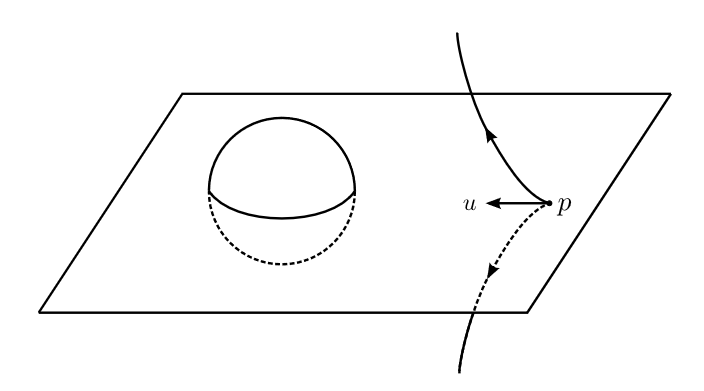
\includegraphics[scale=0.5]{immagini/perassurdo.png}
    \caption{La geodetica deve giacere nello stesso piano altrimenti per simmetria dovrebbe essercene una speculare, generando un assurdo con l'unicità della soluzione noti i dati iniziali.}
    \label{fig.perassurdo}
\end{figure}

Poiché ogni geodetica può essere riportata tramite rotazioni ad una inizialmente equatoriale, possiamo assumere senza perdita di generalità che $\theta = \frac{\pi}{2}$, e ottenere:
\begin{equation*}
    - \varkappa = - \left( 1- \frac{2M}{r}\right) \Dot{t}^2 + \left( 1- \frac{2M}{r}\right)^{-1}\Dot{r}^2 + r^2\Dot{\phi}^2
\end{equation*}

Riscriviamo utilizzando le grandezze conservate dai vettori di Killing, $\Dot{t} = E(1-\frac{2M}{r})^{-1}$ e $\Dot{\phi} = L (r\sin\theta)^{-2}= Lr^{-2}$:
\begin{equation*}
    - \varkappa = -\frac{E^2}{1-\frac{2M}{r}} + \frac{\Dot{r}^2}{1-\frac{2M}{r}} + \frac{L^2}{r^2}
\end{equation*}
cioè riarrangiando:
\begin{equation}
    \frac{E^2}{2} = \frac{\Dot{r}^2}{2} + \frac{1}{2}\left(1-\frac{2M}{r}\right) \left(\frac{L^2}{r^2} + \varkappa \right)
    \label{eq.motoradialegeodschwarz}
\end{equation}

Da un punto di vista classico corrisponde al moto radiale di una particella di massa unitaria non relativistica la quale è sottoposta ad un potenziale efficace:
\begin{align}
    V &= \frac{1}{2}\left(1-\frac{2M}{r}\right) \left(\frac{L^2}{r^2} + \varkappa \right)\nonumber \\
    &=\frac{\varkappa}{2} - \frac{M\varkappa}{r} + \frac{L^2}{2r^2} - \frac{ML^2}{r^3} 
    \label{eq.potenziale_efficace_geodetiche_schwarz}
\end{align}
Osserviamo che tale potenziale è composto da un termine che riconduce al potenziale newtoniano $\frac{M}{r}$, il potenziale centrifugo $\frac{L^2}{2r^2}$ e un ultimo termine di correzione relativistica. Analizziamo quindi il moto al variare di $\varkappa$:
\begin{description}
    \item[Geodetiche tipo tempo]
    Il potenziale assume la forma:
    \begin{equation*}
        V= \frac{1}{2} - \frac{M}{r} + \frac{L^2}{2r^2} - \frac{ML^2}{r^3} 
    \end{equation*}
Ha estremanti per i valori:
    \begin{equation*}
        r_{\pm} = \frac{L^2\pm \sqrt{L^4-12 L^2 M^2}}{2M}
    \end{equation*}
Pertanto se $L^2 < 12M^2$, non ci sono estremi, mentre per $L^2 >12M^2$, $r_+$ è un minimo e $r_-$ è massimo. Questo massimo comporta un'orbita circolare metastabile che non esiste nella teoria newtoniana.
    \item[Geodetiche tipo luce]
    Il potenziale assume la forma:
    \begin{equation*}
        V = \frac{L^2}{2r^2} - \frac{ML^2}{r^3} = \frac{L^2}{r^3}(r-2M)
    \end{equation*}
Si ha un massimo per $r=3M$ a cui corrisponde un'energia pari a $\frac{L^2}{54M^2}$.
\end{description}
I grafici sono mostrati in fig. \ref{fig.geodetiche_schwarz}
\begin{figure}
    \centering
    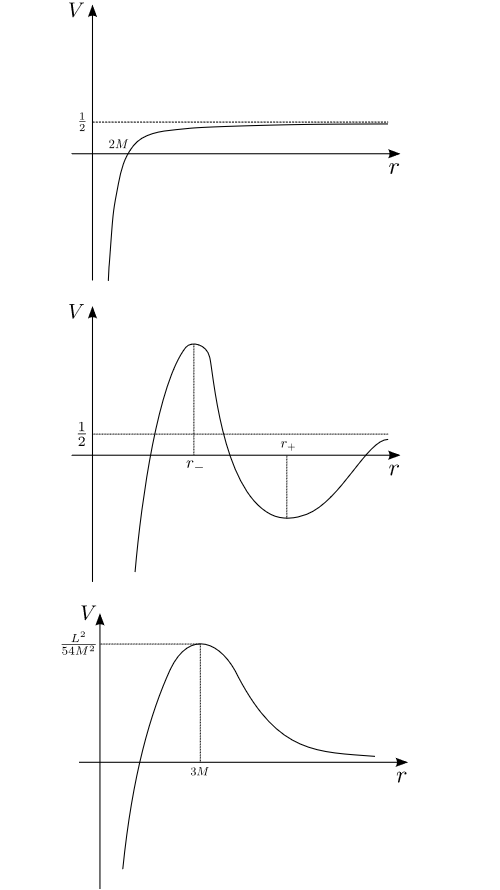
\includegraphics[scale=0.8]{immagini/geodetiche.png}
    \caption{Geodetiche della soluzione di Schwarzschild. Le prime due corrispondo a geodetiche di tipo tempo per $L^2 <12M^2$ e $L^2>12M^2$. L'ultima è la geodetica di tipo luce.}
    \label{fig.geodetiche_schwarz}
\end{figure}
\section{Test classici della relatività generale}
\subsection{Deviazione della luce}
Riprendendo la geodetica di tipo luce prima determinata, si ha per valori di energia
\begin{equation*}
    \frac{E^2}{2} < \frac{L^2}{54M^2}
\end{equation*}
che il moto di un fotone proveniente da infinito, raggiunge un minimo in $r_0$ per poi invertire il suo moto e tornare infinitamente distante, fig. \ref{fig.deflessione}. Questo è il caso di interesse per studiare la deviazione della luce.
\begin{figure}
    \centering
    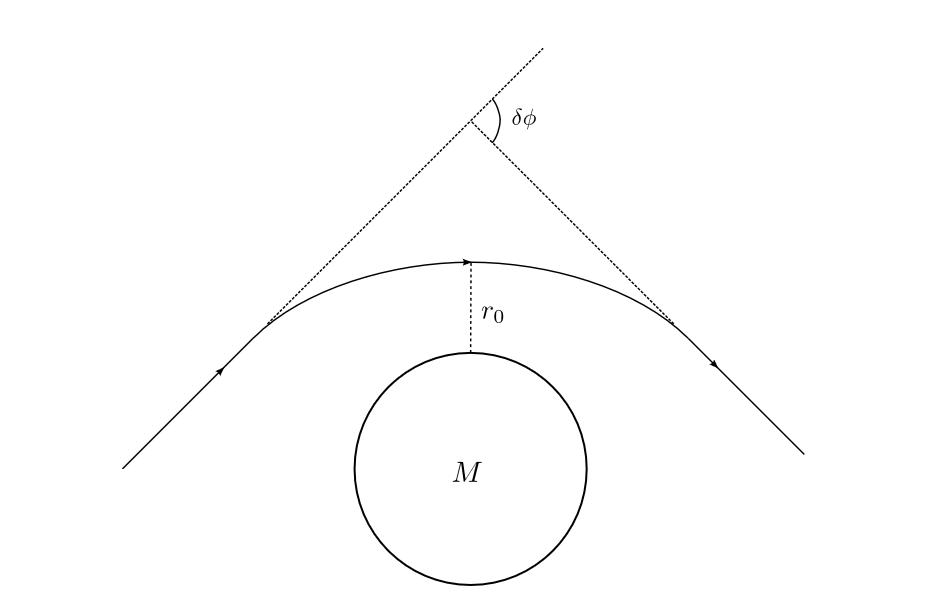
\includegraphics[scale=0.5]{immagini/deflessione.png}
    \caption{Rappresentazione schematica della deflessione della luce.}
    \label{fig.deflessione}
\end{figure}
Definiamo:
\begin{equation*}
    b = \frac{L}{E}
\end{equation*}
detto parametro di impatto apparente. Tale valore in uno spaziotempo piatto corrisponderebbe al parametro di impatto noto nello studio della diffusione, ovvero la distanza minima dall'origine $r=0$; in uno spaziotempo curvo perde questo significato e per tale motivo lo definiamo apparente, sebbene la sua definizione possa rimandare al caso piatto. Questa distanza $r_0$ soddisfa:
\begin{equation*}
    \frac{E^2}{2} = V(r_0) = \frac{L^2}{r_0^3}(r_0 -2M) \iff r_0^3 - b^2(r_0-2M) = 0
\end{equation*}

Consideriamo l'energia del moto radiale eq. \ref{eq.motoradialegeodschwarz}, nel caso della luce cioè con $\varkappa=0$:
\begin{equation*}
    \frac{E^2}{2}= \frac{\Dot{r}^2}{2} + \frac{L^2}{2r^2}-\frac{ML^2}{r^3} \implies \Dot{r}^2 = E^2 - \frac{L^2}{r^2} + \frac{2ML^2}{r^3}
\end{equation*}
Dunque vogliamo esprimere l'angolo al variare del raggio, come in un classico caso di scattering:
\begin{equation*}
    \frac{d\phi}{dr}= \frac{d\phi}{dt}\frac{dt}{dr} = \frac{\Dot{\phi}}{\Dot{r}} = \frac{L}{r^2\sqrt{ E^2 - \frac{L^2}{r^2} + \frac{2ML^2}{r^3} }}
\end{equation*}
Definendo $u=\frac{1}{r}$, si ha $\frac{d\phi}{dr}= \frac{d\phi}{du}\frac{du}{dr} = -\frac{1}{r^2}\frac{d\phi}{du}$ allora:
\begin{equation*}
    \frac{du}{d\phi} = - \frac{1}{L}\sqrt{  E^2 - L^2u^2 +2ML^2u^3    } =- \sqrt{ \frac{1}{b^2} - u^2 +2Mu^3}
\end{equation*}
cioé otteniamo l'equazione differenziale:
\begin{equation}
    u'(\phi)^2 = b^{-2} -u^2 +2Mu^3
    \label{eq.ellitticadeviazioneluce}
\end{equation}
detta \textbf{equazione differenziale ellittica  di Weierstrass}. Come tutte le equazioni differenziali ellittiche, la risoluzione è avanzata e pertanto la risolveremo tramite un metodo perturbativo. Segue:
\begin{equation}
    2u'u" = -2u u' +6Mu^2 u' \implies u" +u = 3Mu^2
    \label{eq.deviazioneluce_perturb}
\end{equation}
Risolviamo il caso imperturbato, cioè in uno spaziotempo piatto con $M=0$; in questo caso i raggi sono delle rette e l'equazione da risolvere è ben nota:
\begin{equation*}
    u" + u = 0 \implies u_0 = C\sin(\phi - \phi_0)
\end{equation*}
Chiamando $u_0$ tale soluzione, si devono imporre le condizioni al contorno che comportano $C=\frac{1}{b}$.

Per risolvere perturbativamente avremo $u= u_0 +\delta u$ che sostituita in eq. \ref{eq.deviazioneluce_perturb} e sfruttando l'identità dell'impertubata:
\begin{equation*}
    u_0"+ \delta u" + u_0 + \delta u = 3M(u_0^2 +(\delta u)^2 +2u_0\delta u)
\end{equation*}
Trascurando inoltre il termine al secondo ordine:
\begin{equation*}
    \delta u" +\delta u =3Mu_0^2 = \frac{3M}{b^2}\sin^2(\phi - \phi_0)
\end{equation*}

Dunque ponendo $\phi_0 = 0$, tale equazione ha soluzione
\begin{equation}
    \delta u = \frac{M}{b^2}(1+ \cos\phi)^2
    \label{eq.deviazione_perturbazione_soluzione}
\end{equation}
così che otteniamo la soluzione totale al primo ordine:
\begin{equation}
    u=\frac{1}{b}\left(  \sin\phi+ \frac{M}{b}(1+\cos\phi)^2 + o(\frac{M}{b})   \right)
    \label{eq.deviazione_totale_soluzione}
\end{equation}

Nel caso del nostro sistema solare $\frac{M}{b} \ll 1$, ed è valido adottare tale soluzione. Il raggio di luce pertanto proviene da infinito e viene deviato dal Sole di un angolo $\delta \phi$ rispetto la direzione incidente e prosegue in traiettoria retta all'infinito; il primo punto (banale) di infinito si ottiene per un angolo $\phi = \pi$ che giustamente comporta $u= 0 \implies r= \infty$. Il secondo punto ad infinito si ottiene sempre annullando $u$, supponendo $\phi_0 = 0$ dell'imperturbata (cioé $\phi = \delta \phi)$:
\begin{equation*}
     \sin\delta\phi+ \frac{M}{b}(1+\cos\delta\phi)^2 = 0
\end{equation*}
ovvero
\begin{equation}
    \delta \phi = - \frac{4M}{b} + o(\frac{M^2}{b^2})
    \label{eq.angolo_deviazione_luce}
\end{equation}
questo corrisponde all'effettivo angolo di deviazione della luce.

\subsection{Redshift gravitazionale}
Consideriamo due osservatori $\mathcal{O}_1$ e $\mathcal{O}_2$, statici, ovvero con quadrivelocità $u_1$, $u_2$ parallele a $\partial_t$: le loro linee di mondo saranno pertanto orbite di $\partial_t$ con posizione $r, \theta, \phi$ fissati, fig. \ref{fig.redshiftgravit}.
Ipotizziamo che $\mathcal{O}_1$ invii dal suo punto $P_1$ un segnale luminoso e che venga ricevuto da $\mathcal{O}_2$ nel punto $P_2$. Il segnale luminoso percorrerà una geodetica di tipo luce per la quale chiamiamo $k^\mu$ il vettore tangente.

\begin{figure}
    \centering
    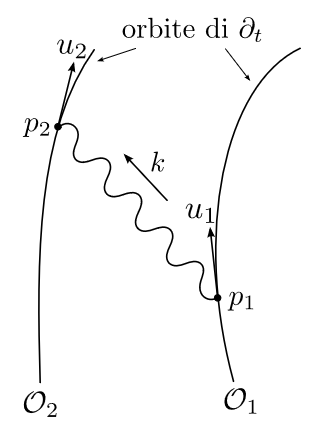
\includegraphics[scale=0.5]{immagini/redshiftgravi.png}
    \caption{Rappresentazione del redshift gravitazionale.}
    \label{fig.redshiftgravit}
\end{figure}
La frequenza di emissione:
\begin{equation*}
    \omega_1 = -k_\mu u^\mu_1 |_{P_1}
\end{equation*}
mentre la frequenza misurata nella ricezione:
\begin{equation*}
    \omega_2 = -k_\mu u^\mu_2 |_{P_2}
\end{equation*}
Poiché le quadrivelocità sono normalizzate, $u_1 ^2 = u_2 ^2 = -1$, e parallele al vettore di Killing $\xi =\partial_t$, potremo scrivere:
\begin{align*}
    u_1^\mu = \frac{\xi^\mu}{(-\xi^2)^{1/2}}\big|_{P_1} &&  u_2^\mu = \frac{\xi^\mu}{(-\xi^2)^{1/2}}\big|_{P_2}
\end{align*}
Si avrà inoltre che
\begin{equation*}
    k \cdot \xi |_{P_1} = k \cdot \xi |_{P_2}
\end{equation*}
poiché lungo la geodetica questa quantità rimane costante. Facendo il rapporto delle frequenze con queste considerazioni si ottiene:
\begin{equation*}
    \frac{\omega_1}{\omega_2} = \frac{ - k_\mu \xi^\mu (-\xi^2)^{-1/2}|_{P_1}}{ - k_\mu \xi^\mu (-\xi^2)^{-1/2}|_{P_2}} = \frac{(-\xi^2)^{-1/2}|_{P_1}}{(-\xi^2)^{-1/2}|_{P_2}}
\end{equation*}
Non resta altro che calcolare il quadrato di $\xi$ nella metrica scelta\footnote{Questa derivazione è valida per un qualsiasi spaziotempo stazionario.}:
\begin{equation*}
    \xi^2 = < \xi, \xi > = < \partial_t, \partial_t > = g_{tt} = - \left( 1-\frac{2M}{r}\right)
\end{equation*}

Otteniamo dunque:
\begin{equation}
    \frac{\omega_1}{\omega_2} = \sqrt{\frac{\left( 1-\frac{2M}{r_2}\right)}{\left( 1-\frac{2M}{r_1}\right)}}
    \label{eq.redshift_frequenze}
\end{equation}

Osserviamo dunque il caso $r_2 > r_1$, cioè l'emettitore più vicino al centro di attrazione gravitazionale, allora si avrà $\omega_2 < \omega_1$ altresì $\lambda_2 > \lambda_1$: la lunghezza d'onda misurata è più lunga rispetto quella emessa, cioè ha subito uno \emph{spostamento verso il rosso} o \emph{redshift}. In altri termini, l'energia del fotone $E=\hbar \omega$ è diminuita poiché è passata in una regione a maggiore potenziale gravitazionale.

Se analizziamo il limite $M \ll r_1, r_2$, eseguendo le opportune approssimazioni con sviluppi di Taylor ed esplicitando le costanti prima mantenute unitarie:
\begin{equation*}
    \frac{\Delta \omega}{\omega} \approx - \frac{GM}{c^2r^1} + - \frac{GM}{c^2r^2} \iff \hbar \Delta \omega \approx \frac{\hbar \omega}{c^2}\left( - \frac{GM}{r^1} + - \frac{GM}{r^2}\right)
\end{equation*}
risulta evidente come la differenza di energia del fotone sia dovuta alla differenza del potenziale gravitazionale newtoniano tra i punti iniziali e finali.

L'effetto fu sperimentalmente verificato nel 1959 da R. Pound e G. Rebka, sfruttando l'effetto Mössbauer nell'emissione di raggi gamma (cioè senza rinculo) da parte di un nucleo di $^{57}$Fe.
Chiariamo infine che questo effetto doppler è ben diverso da quello relativistico, emerso nella relatività ristretta, e trae origine nel principio di equivalenza e nella dilatazione temporale nei pressi del pozzo gravitazionale (la sorgente del campo); è l'effetto doppler che insieme a quello relativistico, vanno tenuti in considerazione nella progettazione dei sistemi di navigazione satellitare. Con osservatore ed emettitore lontani dalle sorgenti di campo, in regime di metrica piatta, il redshift gravitazionale è evidentemente trascurabile.

Esisterà poi un altro tipo di redshift dovuto invece alla struttura dell'universo e alla sua espansione.


\subsection{Precessione del perielio}
Riprendendo i calcoli delle geodetiche di tipo tempo:
\begin{equation*}
    \left(\frac{dr}{d\phi}\right)^2 = \frac{\Dot{r}^2}{\dot{\phi}^2} = \frac{E^2 -1 +\frac{2M}{r} - \frac{L^2}{r^2} + \frac{2ML^2}{r^3}}{\frac{L^2}{r^4}}
\end{equation*}
Introducendo la variabile $u=r^{-1}$ e il parametro d'urto apparente $b = \frac{L}{E}$:
\begin{equation*}
    \left(\frac{du}{d\phi}\right)^2 = b^{-2} - L^{-2} + \frac{2M}{L^2}u - u^2 +2Mu^3 
\end{equation*}
Derivando una volta e semplificando:
\begin{equation*}
    2u'u" = \frac{2M}{L^2} u' - 2u u' +6Mu^2u'
\end{equation*}
otteniamo
\begin{equation}
    u"(\phi) = \frac{M}{L^2} +3Mu^2(\phi) - u(\phi)
    \label{eq.diff_perielio}
\end{equation}
Osserviamo che questa equazione differenziale, rispetto al caso newtoniano, differisce per il termine $3Mu^2$. La sua soluzione esatta è una funzione ellittica, pertanto la risolveremo perturbativamente, così come si è già fatto. I termini di validità dell'approccio perturbativo saranno chiariti in seguito. 

L'equazione imperturbata fornisce la soluzione del problema di Keplero:
\begin{equation}
    u" +u = \frac{M}{L^2} \implies u_0 = \frac{M}{L^2} (1+\epsilon\cos\phi)
    \label{eq.imperturbata_keplero}
\end{equation}
Cercando soluzioni $u= u_0 + \delta u$ in eq. \ref{eq.diff_perielio} e trascurando termini al secondo ordine:
\begin{align}
    u_0" +\delta u" + u_0 + \delta u = \frac{M}{L^2} + 3M(u_0^2+ (\delta u)^2 +2u_0 \delta u) \nonumber \\
    \implies \delta u" + \delta u = 3M u_0^2
    \label{eq.diff_perielio_perturb}
\end{align}
L'approccio perturbativo risulta valido quando $Mu = \frac{M}{r} \ll 1$. Attraverso il metodo della variazione delle costanti si risolve eq. \ref{eq.diff_perielio_perturb} ricavando:
\begin{equation}
    \delta u = \frac{3M^3}{L^4}\left(1 + \epsilon \phi \sin \phi + \epsilon^2(\frac{1}{2} -\frac{1}{6}\cos(2\phi) )\right)
\end{equation}

Il metodo perturbativo ci fornisce dunque:
\begin{equation*}
     u = u_0 + \frac{3M^3}{L^4}\left(1 + \epsilon \phi \sin \phi + \epsilon^2(\frac{1}{2} -\frac{1}{6}\cos(2\phi) )\right)
\end{equation*}
Questa non è più periodica e inoltre possiede un termine dominante illimitato, $\phi\sin\phi$. Trascurando le altre correzioni:
\begin{equation*}
    u = \frac{M}{L^2}\left( 1+\epsilon\cos\phi + \epsilon\frac{3M^2}{L^2}\phi\sin\phi\right)
\end{equation*}
e applicandola al caso $\frac{M}{L} \ll 1$ (questo è ben soddisfatto nel caso solare):
\begin{equation}
    u \approx \frac{M}{L^2}\left( 1+\epsilon\cos((1-3\frac{3M^2}{L^2})\phi)\right)
\end{equation}
In questa approssimazione, la soluzione è nuovamente periodica, ma non più di $2\pi$; non descrive orbite chiuse, ma che precedono al perielio di un angolo $\Delta \phi$ pari a:
\begin{equation}
    \Delta \phi = \frac{2\pi}{1-\frac{3M^2}{L^2}} \approx 2\pi\left(1+\frac{3M^2}{L^2}\right)
    \label{eq.precessione}
\end{equation}
\begin{figure}
    \centering
    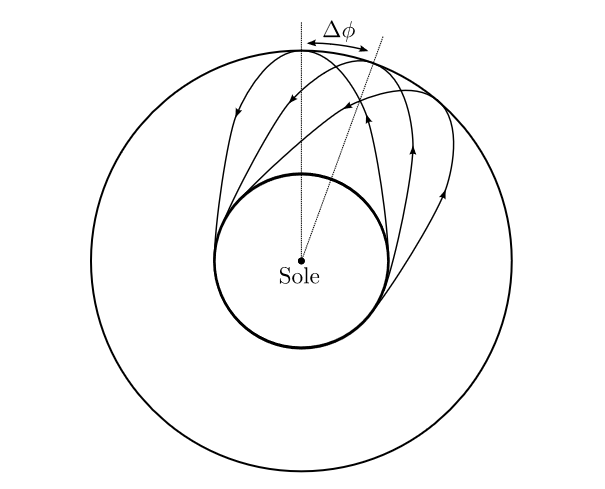
\includegraphics[scale=0.5]{immagini/precessione.png}
    \caption{Rappresentazione schematica della precessione di Mercurio.}
    \label{fig.precessione}
\end{figure}

\section{Estensione di Kruskal}\label{para.kruskal}
Sebbene il concetto di buco nero e orizzonte degli eventi fossero già stati descritti agli albori della relatività generale, dopo che era stata formulata la soluzione di Schwarzschild, si deve a Martin D. Kruskal, in parallelo a George Szekeres, nel 1960, il lavoro che ha permesso di descrivere in maniera completa la singolarità della metrica.
Le prime discussioni di un buco nero in tale metrica erano limitate a descrivere la sola regione al di fuori dell'orizzonte degli eventi (il significato di tale termine sarà poi chiarito); come vedremo quella che prende il nome di \emph{estensione di Kruskal}, fornisce una descrizione più completa e ha permesso l'introduzione di ulteriori concetti quali il \emph{buco bianco} o il \emph{ponte di Einstein-Rosen}.

Riprendendo la soluzione di Schwarzschild, eq. \ref{eq.metricaschwarz}, possiamo vedere come in $r= 2M$, ovvero per il cosiddetto raggio di Schwarzschild, la metrica sia singolare con $g_{tt}\rightarrow 0$ e $g_{rr}\rightarrow+\infty$. Questa non è una \textbf{singolarità di curvatura}, come invece è $r=0$. Ad esempio l'invariante di curvatura:
\begin{equation*}
    R_{\mu\nu\rho\sigma} R^{\mu\nu\rho\sigma} \propto \frac{1}{r^2}
\end{equation*}
detto \emph{scalare di Kretschmann}, è singolare in $r=0$, non in $r=2M$. Il raggio di Schwarzschild è invece una \textbf{singolarità delle coordinate}.

Da un punto di vista fisico, per ogni configurazione statica all'equilibrio, la regione $r\leq 2M$ è interna alla distribuzione di materia e pertanto la sua discussione non è rilevante allo studio del campo gravitazionale di, ad esempio, una stella statica.  Corpi sufficientemente massivi invece, quando esauriscono gli elementi che mantengono attiva la fusione nucleare che avviene in essi e che compensa l'attrazione dovuta all'enorme materia, vanno incontro ad un collasso gravitazionale il quale può portarli ad una supernova, una stella di neutroni o ad un buco nero. In questi casi tale regione diventa rilevante allo studio.

L'idea alla base dell'estensione di Kruskal è che se si considerano le geodetiche, che siano tipo tempo o luce, tendenti alla singolarità $r=2M$, queste vi arrivano con parametro affine finito. Il punto non è all'infinito e ciò suggerisce di assumere tale parametro come nuova coordinata.

Osserviamo che in generale nuove singolarità di coordinate si introducono qualora delle geodetiche si intersechino; tuttavia in due dimensioni, almeno localmente, le geodetiche nulle si dividono in \emph{outgoing} e \emph{ingoing}\footnote{Tali geodetiche sono caratterizzate da $t\pm r = \textrm{cost.}$; col segno $+$ si ha che aumentando $t$, deve diminuire $r$ quindi la geodetica \virgolette{si avvicina} (ingoing). Viceversa con l'altro segno.} e dentro tali classi non sono possibili intersezioni. Le coordinate ricercate saranno costanti lungo queste geodetiche. La corrispondente griglia di coordinate sarà quindi basata sulla geometrica \virgolette{griglia} di geodetiche nulle.

Partiamo studiando la metrica bidimensionale (la parte angolare rimane immutata nella simmetria centrale):
\begin{equation*}
    ds^2 = - \left( 1 - \frac{2M}{r}\right) dt^2 +  \left( 1 - \frac{2M}{r}\right)^{-1} dr^2
\end{equation*}
considerando le geodetiche nulle, $ds^2=0$, ovvero la luce, otteniamo:
\begin{equation*}
    dt =  \pm \left( \frac{r}{r-2M}\right) dr
\end{equation*}
Integrando:
\begin{equation*}
    t = \pm r_* + \textrm{cost.}
\end{equation*}
dove $r_* = r+2M\log(\frac{r}{2M}-1)$; questa è chiamata \textbf{coordinata tartaruga di Regge-Wheeler}\footnote{Il nome si rifà al paradosso di Zeno di Achille e la tartaruga; \virgolette{Sfortunatamente Zeno non sapeva che la serie geometrica fosse convergente}. Infatti $r$ varia lentamente, variando $r_*$ poiché $\frac{dr}{dr_*}\rightarrow 0$ per $r\rightarrow2M$.}. Introducendo le coordinate outgoing e ingoing\footnote{Le coordinate \virgolette{ibride} $(u,r)$ o $(v,r)$ sono dette \emph{coordinate di Eddington-Finkelstein}.}:
\begin{equation*}
    \left\{\begin{array}{c}
         u = t - r_* \\
         v = t + r_*
    \end{array}\right.
\end{equation*}
la metrica diventa:
\begin{equation*}
    ds^2 = -  \left( 1 - \frac{2M}{r}\right)dudv
\end{equation*}
Questa mantiene ancora la singolarità $r=2M$. Qui $r$ è funzione delle $u, v$ implicitamente secondo:
\begin{equation*}
    r_*(r)= \frac{v-u}{2}
\end{equation*}
Rielaboriamo la metrica riscrivendo:
\begin{equation*}
    -\left( 1 - \frac{2M}{r}\right) = - \frac{2M}{r}\left( \frac{r}{2M}-1\right)
\end{equation*}
e inoltre:
\begin{equation*}
    \frac{r_*}{2M} = \frac{r}{2M}+\log(\frac{r}{2M}-1) \implies e^{r_*/2M} = e^{r/2M}\left(\frac{r}{2M}-1\right) \implies \left(\frac{r}{2M}-1\right) =  e^{r_*/2M} e^{-r/2M}
\end{equation*}
Comporta:
\begin{equation*}
    ds^2 = - \frac{2M}{r}\exp({-\frac{r}{2M}}) \exp({\frac{v-u}{4M}})dudv
\end{equation*}
Questa metrica è ancora singolare in $r=2M$ cioè $r_*\rightarrow-\infty$ a cui corrispondono $u\rightarrow -\infty$ e $v \rightarrow +\infty$. Tuttavia ci suggerisce le nuove coordinate:
\begin{align}
    U= - e^{-u/4M} && V= e^{v/4M}
\end{align}
dette \textbf{coordinate di Kruskal-Szekeres}. Queste, come da idea iniziale, sono parametri affini per le geodetiche nulle considerate. Osserviamo inoltre che per loro definizione $U<0$ e $V>0$, mentre la singolarità $r=2M$ corrisponde a $U=V=0$. 
Ricalcolando:
\begin{equation*}
    \left\{\begin{array}{l}
    dU = -\frac{U}{4M}du \\ \\
    dV = \frac{V}{4M}dv
    \end{array}\right.  \implies dudv = - 16M^2 \exp{(-\frac{v-u}{4M})}dUdV
\end{equation*}
e la metrica diventa:
\begin{equation}
    ds^2 = -\frac{32M^3 e^{-r/2M}}{r}dUdV
    \label{eq.metrica_kruskal_UV}
\end{equation}
Questa metrica \textbf{non è più singolare} e ci permette di estendere la soluzione di Schwarzschild a tutti i valori $U<0, V>0$ compatibili con $r>0$. Per quanto detto inizialmente, non si può andare con valori oltre $r=0$ perché questo punto rappresenta una singolarità di curvatura.

Effettuiamo infine la trasformazione:
\begin{align}
    T=\frac{U+V}{2} && X=\frac{V-U}{2}
    \label{eq.coordinateTX_kruskal}
\end{align}
così che $dU=dT+dX$ e $dV=dT-dX$ e si ottiene la metrica finale\footnote{Si può fare un'analoga derivazione, che risulta formalmente identica a questa, a partire dalla metrica di Rindler $ds^2 = -x^2dt^2 + dx^2$ che ci permette di dire che l'estensione dello spaziotempo di Rindler è lo spaziotempo di Minkowski.} (riportando anche la parte angolare):
\begin{equation}
    ds^2 = \frac{32M^3 e^{-r/2M}}{r}( - dT^2 + dX^2) + r^2(d\theta^2 + \sin^2\theta d\phi^2)
    \label{eq.metrica_kruskal}
\end{equation}
a meno di un prefattore (che diventa ininfluente per geodetiche nulle), i primi due termini in $T, X$ non sono altro che la metrica di Minkowski, mentre la parte restante è dovuta alla simmetria centrale. Pertanto in un piano $(X,T)$ ogni punto non è altro che una 2-sfera. Esprimiamo la relazione tra le coordinate iniziali $(t,r)$ e $(T,X)$:
\begin{equation}
    \left\{ \begin{array}{l}
          \left(\frac{r}{2M}-1\right) e^{r/2M} = X^2 - T^2 \\
          \frac{t}{2M}= 2\arctanh (\frac{T}{X})
    \end{array}\right.
\end{equation}
In questo modo possiamo rappresentare:
\begin{itemize}
    \item $r=\textrm{cost.} \implies X^2 - T^2 = \textrm{cost.}$ ovvero  un'iperbole.
    \item $r=2M \implies X^2 = T^2$ ovvero le bisettrici.
    \item $t=\textrm{cost.} \implies \frac{T}{X} = \textrm{cost.}$ ovvero delle rette.
    \item $r>0 \implies X^2-T^2 > -1$ ovvero il range di soluzioni permesse.
\end{itemize}
Con queste possiamo quindi rendere graficamente lo spaziotempo di Schwarzschild esteso in presenza di un buco nero come in fig. \ref{fig.kruskal}.
\begin{figure}
    \centering
    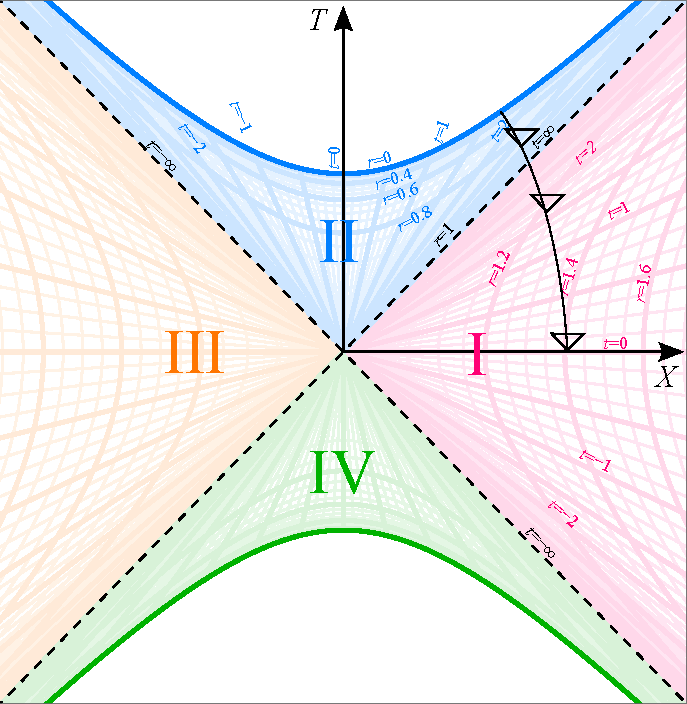
\includegraphics[scale=0.8]{immagini/kruskal.pdf}
    \caption{Spaziotempo di Schwarzschild nell'estensione di Kruskal. Ogni punto del piano rappresenta una 2-sfera. Viene rappresentato un evento che superando l'orizzonte degli eventi, cioè entrando nella regione II, non può più uscirne in quanto la velocità massima che può raggiungere, pari a $c$, non è sufficiente a tagliare la bisettrice (il cono dovrebbe avere un angolo maggiore di 45 gradi).}
    \label{fig.kruskal}
\end{figure}
Per quanto detto sul prefattore della metrica, essendo ininfluente per geodetiche luce, si avrà che i coni di luce saranno comunque a 45 gradi.
Vengono riconosciute 4 regioni; analizziamole:
\begin{description}
    \item[Regione I] corrispondente a $r> 2M$, è la regione asintoticamente piatta che descrive il campo gravitazionale al di fuori della distribuzione di materia sferica.
    \item[Regione II] corrispondente al \textbf{buco nero}, infatti un qualsiasi osservatore che oltrepassi radialmente la bisettrice $X=T$ sarà destinato a cadere nella singolarità rappresentata dalla regione delimitata dall'iperbole superiore. Qualsiasi segnale luminoso inviato dalla regione II sarà destinato a rimanere intrappolato in essa in quanto per intersecare nuovamente la bisettrice, bisognerebbe avere un segnale luminoso con angolo maggiore di 45 gradi, il che non è possibile. La caduta nella singolarità avviene in un intervallo di tempo proprio finito. La bisettrice $X=T$ è chiamata $H^+$ oppure \textbf{orizzonte degli eventi}.
    \item[Regione III] corrispondente ad un altro universo asintoticamente piatto che giace \virgolette{all'interno} del \virgolette{raggio} $r=2M$.
    \item[Regione IV] corrispondente al \textbf{buco bianco}. \'E una regione con il \virgolette{tempo rovesciato} rispetto la regione II. Qualsiasi osservatore all'interno di essa deve necessariamente provenire dalla singolarità $r=0$ e uscirne, attraversando la bisettrice $X=-T$, in un tempo proprio finito. La bisettrice è detta $H^-$ oppure \textbf{orizzonte del passato}.
\end{description}

Per capire la geometria che collega le due regioni I, III si considera la superficie di tipo spazio $T=0$.
La metrica indotta su questa superficie è:
\begin{equation*}
    ds^2 = \left( 1- \frac{2M}{r}\right)^{-1} dr^2 + r^2(d\theta^2 + \sin^2\theta d\phi^2)
\end{equation*}
Grazie alla simmetria sferica possiamo limitarci a discutere il piano equatoriale $\theta= \frac{\pi}{2}$:
\begin{equation}
    ds^2 = \left( 1- \frac{2M}{r}\right)^{-1} dr^2 +r^2 d\phi^2
    \label{eq.metrica_ponte}
\end{equation}
Per visualizzare questa superficie 2-dim., la immergiamo nello spazio euclideo $\mathbb{E}^3$. La metrica standard di $\mathbb{E}^3$ in coordinate cilindriche è:
\begin{equation*}
    ds^2 = dz^2 +dr^2 +r^2d\phi^2
\end{equation*}
Se si considera $z=z(r)$, quindi una superficie di rotazione di $\mathbb{E}^3$, tale metrica indotta su questa superficie è:
\begin{equation*}
    ds^2 = \left[ 1+ \left( \frac{dz}{dr}\right)^2 \right]dr^2 +r^2d\phi^2
\end{equation*}
Abbiamo quindi tutti gli elementi per confrontarla con eq. \ref{eq.metrica_ponte} e visualizzare l'embedding reso possibile da:
\begin{equation*}
    r= 2M + \frac{z^2}{8M}
\end{equation*}
Questo viene chiamato \textbf{ponte di Einstein-Rosen}.
La topologia di tale superficie è $\mathbb{R}\times S^2$; nel grafico una dimensione è necessariamente soppressa, pertanto ogni cerchio rappresenta in realtà una 2-sfera.
Osserviamo inoltre che non è possibile comunicare tra queste due regioni proprio perché qualsiasi segnale luminoso inviato, cadrebbe nel buco nero.

L'estensione di Kruskal descrive uno spaziotempo con buco nero eterno e nel quale compaiono due universi tra loro legati dalla singolarità. In generale non c'è ragione per credere che tale configurazione iniziale sia quella di ogni parte nel nostro universo e pertanto non c'è motivo per pensare che ogni regione dell'universo corrisponda alla completa estensione della soluzione di Schwarzschild. Inoltre se si considera il meccanismo che può portare alla formazione di un buco nero -- collasso gravitazionale --, le regioni III, IV, non si formano nemmeno.

Un corpo sufficientemente massivo che va incontro ad un collasso gravitazionale completo avrà una metrica interna ad esso che non potrà essere quella di Schwarzschild, in quanto $T_{\mu\nu}\neq 0$; tuttavia se consideriamo la regione esterna ad esso, vale Schwarzschild poiché, come visto dal teorema di Birkhoff, è l'unica soluzione a simmetria sferica nel vuoto. Le regioni III, IV sarebbero \virgolette{coperte} dalla materia dell'oggetto in collasso, mentre la regione II verrebbe a crearsi qualora la coordinata radiale diventasse minore di $2M$.

\section{Coordinate di Painlevè-Gullstrand per moto di caduta libera}
Consideriamo un osservatore di tipo tempo in caduta libera nella geometria di Schwarzschild, eq. \ref{eq.metricaschwarz}. Il moto avviene con $\theta, \phi$ costanti e considerando come condizione iniziale $\dot{r}= 0$ per $r\rightarrow + \infty$, ovvero che il moto parta con velocità nulla.

Riprendendo i calcoli effettuati in \S\ref{para.geodschwarz}, il vettore tangente alla geodetica $u^\mu = \frac{d x^\mu}{d\tau} =: x^\mu$ (parametrizzata con tempo proprio) si conserva lungo la stessa e ci ha permesso di scrivere:
\begin{equation*}
    u_\mu(\partial_t)^\mu = - E \implies \dot{t} = E\left( 1 - \frac{2M}{r}\right)^{-1}
\end{equation*}
La condizione di normalità della quadrivelocità ha comportato (considerando $\theta,\phi$ costanti):
\begin{equation}
    -\left( 1 - \frac{2M}{r}\right)\dot{t}^2 + \left( 1 - \frac{2M}{r}\right)^{-1}\dot{r^2} = -1
    \label{eq.normalizza_gullstrand}
\end{equation}
Sostituendo $\dot{t}$ in quest'ultima e riarrangiando otteniamo:
\begin{equation*}
    \dot{r}^2 = E^2 -1 +\frac{2M}{r}
\end{equation*}

Poiché $E$ è costante lungo la geodetica, il suo valore viene determinato dalle condizioni iniziali a $r\rightarrow +\infty$ per le quali si ha $\dot{r}= 0 \implies p = 0$. In questo modo:
\begin{equation*}
    E = \sqrt{p^2 + m^2} \implies E = 1
\end{equation*}
considerando $m = 1$ la massa dell'osservatore test. Pertanto:
\begin{align}
    \dot{t} = \left( 1 - \frac{2M}{r}\right)^{-1} && \dot{r}^2 = \frac{2M}{r}
    \label{eq.dot_gull}
\end{align}

Nell'ipotesi $\dot{r}< 0$ i.e. $\dot{r} = - \sqrt{\frac{2M}{r}}$, se sostituiamo una volta eq. \ref{eq.dot_gull} in eq. \ref{eq.normalizza_gullstrand}, otteniamo:
\begin{equation*}
    \dot{t} + \sqrt{\frac{2M}{r}}\left( 1 - \frac{2M}{r}\right)^{-1}\dot{r} = 1
\end{equation*}
Richiamando $\frac{d x^\mu}{d\tau}$:
\begin{equation}
    dt + \sqrt{\frac{2M}{r}}\left( 1 - \frac{2M}{r}\right)^{-1} dr = d\tau
    \label{eq.dtau_gull}
\end{equation}
ovvero
\begin{equation*}
    \tau = t  + \int_{+\infty}^{r} \sqrt{\frac{2M}{r'}}\left( 1 - \frac{2M}{r'}\right)^{-1} dr'
\end{equation*}

Se usassimo $\tau$ come nuova variabile temporale e sostituissimo $dt$ da eq. \ref{eq.dtau_gull} in eq. \ref{eq.metricaschwarz}, svolgendo il quadrato e semplificando, otterremmo:
\begin{equation}
    ds^2 = - \left( 1 - \frac{2M}{r}\right) d\tau^2 + 2\sqrt{\frac{2M}{r}}d\tau dr + dr^2 + r^2(\sin^2\theta d\phi^2 + d\theta^2)
    \label{eq.metrica_paingull}
\end{equation}
Questa è detta \textbf{metrica di Painlevé-Gullstrand}; si può notare che è stazionaria, ma non statica. Notiamo inoltre che le ipersuperfici $\tau = \textrm{cost.}$ riducono la metrica a quella di $\mathbb{E}^3$, cioè sono ipersuperfici piatte.
\chapter{Cosmologia di Friedmann-Lema\^itre-Robertson-Walker}\label{para.cosmo}
La cosmologia ha come scopo la descrizione dell'universo nel suo insieme, cercando di spiegarne l'origine e l'evoluzione. Scopo di questa sezione è determinare quali soluzioni alle equazioni di Einstein sono idonee alla descrizione dell'universo e sotto quali ipotesi avvengono. Verrà fatta un'overview generale degli aspetti fondamentali legati alla cosmologia FLRW, per la descrizione di un universo omogeneo e isotropo.

\section{Omogeneità e isotropia}
All'interno del modello cosmologico si assumono le ipotesi che esso sia \emph{omogeneo} e \emph{isotopo}. Da un punto di vista storico già dagli studi di Copernico si è consolidata l'idea che la posizione nell'universo non fosse privilegiata. Se ci trovassimo in un'altra regione dell'universo le caratteristiche di base del nostro intorno sarebbero le stesse. Un universo omogeneo è un universo indipendente dalla posizione.

Similmente non ha senso assumere che esistano direzioni privilegiate, da cui l'ipotesi dell'isotropia. \'E importante osservare che queste ipotesi di carattere filosofico sono comunque supportate sperimentalmente: in particolare su grandi scale si è osservato che la distribuzione delle galassie è isotropa e omogenea (nonostante a scale minori si possano osservare \emph{clusters} di galassie e regioni prive di esse) ed inoltre gli studi sulla radiazione cosmica di fondo (CMB) hanno riportato analoghi risultati.

Esprimiamo rigorosamente l'omogeneità e l'isotropia:
\begin{definizione}
Uno spaziotempo $\mathcal{M}$ è (spazialmente) \textbf{omogeneo} se esiste una famiglia ad un parametro di ipersuperfici $\Sigma_t$ di tipo spazio tali che
\begin{equation*}
    \bigcup_t \Sigma_t = \mathcal{M}
\end{equation*}
e $\forall t$, $\forall p,q \in \Sigma_t$ esiste sempre un'isometria $f$ della metrica $g_{\mu\nu}$ tale che $f(p)=q$ cioè che mappa uno nell'altro.
\end{definizione}

\begin{definizione}
Uno spaziotempo $\mathcal{M}$ è (spazialmente) \textbf{isotropo} in ogni punto se esiste una congruenza di curve di tipo tempo con vettori tangenti $u$ tali che:
\begin{enumerate}
    \item Lo spaziotempo $\mathcal{M}$ è unione delle curve.
    \item Dato $p$ qualsiasi e due vettori $s_1, s_2 \perp u$ in $p$, esiste sempre un'isometria che lascia $p,u$ invariati e ruota $s_1$ in $s_2$.
\end{enumerate}
\end{definizione}

Quest'ultimo punto è quello che permette di dire che non ci sono vettori spaziali preferiti ovvero che non si può costruire vettore perpendicolare a $u$ che sia geometricamente privilegiato.

Come conseguenza di queste definizioni, in un universo omogeneo e isotropo le ipersuperfici $\Sigma_t$ devono essere perpendicolari ai vettori tangenti $u$, altrimenti proiettando quest'ultimo sull'ipersuperficie si potrebbe costruire un vettore geometricamente preferito.

Con queste considerazioni si ha che la metrica $g_{\mu\nu}$ induce sulla ipersuperficie (3-dimensionale) $\Sigma_t$ una metrica $h_{\mu\nu}(t)$ (vale a dire restringere $g$ ai vettori tangenti alla superficie).
\begin{align*}
    g_{\mu\nu} = -u_\mu u_\nu +h_{\mu\nu}(t)  \overset{\cdot u^\nu}{\longrightarrow} g_{\mu\nu} u^\nu &= -u_\mu u_\nu u^\nu + h_{\mu\nu}(t)u^\nu \\
     u_\mu &= u_\mu + h_{\mu\nu}(t)u^\nu
\end{align*}
ciò implica $ h_{\mu\nu} u^\nu = 0$ (proiettore) e che $u$ sia autovettore di $h$ con autovalore nullo. Segue che possiamo esprimere la matrice di $h$ almeno nella forma:
\begin{equation*}
    h_{\mu\nu}(t) =
  \begin{pmatrix}
  0 & 0 & 0& 0 \\
  0& & & & \\
  0& &   h_{ij}(t)& & \\
  0& & & &
  \end{pmatrix}
\end{equation*}

cioè isolando in un blocco tale autovalore, e lasciando indeterminata la restante matrice 3x3. Vediamo ora quali conseguenze su $h_{ij}$ comportano l'omogeneità e l'isotropia.

Consideriamo il tensore di Riemann costruito sulla metrica $h_{ij}$: $\tensor{R}{^i_{jkl}}$. Questo viene alzato da $h$ in $\tensor{R}{^{ij}_{kl}}$ antisimmetrico nello scambio delle coppie $ij$, $kl$ per via delle proprietà generali del tensore. Pertanto si ha l'applicazione lineare:
\begin{align*}
    L : W &\rightarrow W \\
    \omega_{ij} &\mapsto \tilde{\omega}_{kl} =\tensor{R}{^{ij}_{kl}}\omega_{ij}
\end{align*}
dove $W$ è lo spazio vettoriale delle 2-forme. Poiché $\tensor{R}{^{ij}_{kl}} = \tensor{R}{_{kl}^{ij}}$ sempre per le proprietà del tensore, allora l'applicazione $L$ è simmetrica e pertanto ammette base ortonormale di autovettori.

Per l'ipotesi sulla isotropia, tutti gli autovalori di L devono essere uguali e quindi $L$ risulta multiplo dell'identità:
\begin{equation*}
    L = k \mathds{1}
\end{equation*}
Infatti se così non fosse, supponiamo si abbiano gli autovalori $\lambda_1, \lambda_2 = \lambda_3$, si avrebbe per il primo l'autovettore $\omega^{(1)}_{ij}$ che determina il vettore spaziale $v^k = \epsilon^{ijk}\omega^{(1)}_{ij}$. Questo sarebbe un vettore spaziale preferito e quindi contro l'isotropia.

L'omogeneità implica invece che $k$ non dipenda dalla posizione, ma al massimo dal tempo. Si ottiene quindi il tensore di Riemann (di dim. 3) costruito sulla metrica indotta sulle ipersuperfici di tipo spazio $\Sigma_t$:
\begin{equation}
    \tensor{R}{^{ij}_{kl}} = k \tensor{\delta}{^i_{[k}} \tensor{\delta}{^j_{l]}}
    \label{eq.R_curva_cost}
\end{equation}
L'antisimmetrizzazione sugli indici delle $\delta$ è inserita per mantenere l'antisimmetria del tensore a sinistra.

Osserviamo che $k= \textrm{cost.}$ segue anche dalla seconda identità di Bianchi: $\tensor{R}{^{ij}_{[jk;m]}}=0$. Esplicitamente su \cite{wald}. Questo comporta che si potrebbe fare anche a meno dell'ipotesi sull'omogeneità, ma è anche da osservare che la richiesta di isotropia in ogni punto implica essa stessa l'omogeneità.

\begin{definizione}
Uno  spaziotempo $\mathcal{M}$ che soddisfa eq. \ref{eq.R_curva_cost} si dice \textbf{a curvatura costante}.
\end{definizione}

Mostriamo che per uno spazio a curvatura costante vale eq. \ref{eq.riemann_curvatura_costante}. Il calcolo è abbastanza diretto, dovendo soltanto abbassare i primi due indici:
\begin{equation*}
    R_{\mu\nu\rho\sigma} = g_{\mu\alpha}g_{\nu\beta} \tensor{R}{^{\alpha\beta}_{\rho\sigma}} = kg_{\mu\alpha}g_{\nu\beta}(\tensor{\delta}{^\alpha_\rho}\tensor{\delta}{^\beta_\sigma} - \tensor{\delta}{^\alpha_\sigma}\tensor{\delta}{^\beta_\rho}) = k(g_{\mu\rho}g_{\nu\sigma} - g_{\mu\sigma}g_{\nu\rho})
\end{equation*}

Facciamo vedere inoltre che per tale spazio si può esprimere $k$ in funzione dello scalare di Ricci secondo eq. \ref{eq.costvettorikillinglambda}. Per fare questo ricordiamo che la traccia dell'identità è pari alla dimensione dello spazio, ovvero $\tensor{\delta}{^\sigma_\sigma} = n$. Calcoliamo il Ricci da eq. \ref{eq.R_curva_cost}:
\begin{align*}
    \tensor{R}{^\nu_\sigma} &= \tensor{R}{^{\mu\nu}_{\mu\sigma}} = k(\tensor{\delta}{^\mu_\mu}\tensor{\delta}{^\nu_\sigma} - \tensor{\delta}{^\mu_\sigma}\tensor{\delta}{^\nu_\mu}) \\
    &= k(n\tensor{\delta}{^\nu_\sigma} - \tensor{\delta}{^\mu_\sigma}\tensor{\delta}{^\nu_\mu}) =k(n-1)\tensor{\delta}{^\nu_\sigma}
\end{align*}
Quindi lo scalare di Ricci:
\begin{equation*}
    R = \tensor{R}{^\sigma_\sigma} = k(n-1)\tensor{\delta}{^\sigma_\sigma} = k n(n-1)
\end{equation*}

Poiché l'ipersuperficie di omogeneità $\Sigma_t$ è di dimensione 3, si avrà che $R=6k$.
\section{Metrica FLRW}

Si deve a Luther P. Eisenhart nel 1949 la classificazione degli spazi a curvatura costante di dimensione $n$ e con segnatura $n$ (quindi tutti autovalori positivi della metrica). Tali spazi sono isometrici a:
\begin{itemize}
    \item $H^n$ spazio iperbolico se $k<0$.
    \item $\mathbb{E}^n$ spazio euclideo se $k=0$.
    \item $S^n$ $n$-sfera se $k>0$.
\end{itemize}
La geometria spaziale dell'universo è una di queste tre. Nella fisica prerelativistica, così come nella relatività ristretta, si assume uno spazio piatto, $k=0$; è interessante notare come le richieste più restringenti di omogeneità e isotropia permettano di avere ulteriori due possibilità.

Aspetto fondamentale dello spazio $S^n$ è che descrive un universo chiuso, cioè finito, ma senza bordo (un palloncino è finito, ma non ha un bordo), mentre lo spazio piatto e iperbolico sono aperti.

La metrica di $S^3$ è:
\begin{equation}
    ds^2 = l^2(d\psi^2 +\sin^2\psi( d\theta^2 + \sin^2\theta d\phi^2))
    \label{eq.metrica_s3}
\end{equation}
definendo il termine tra parentesi $(d\Omega_1)^2$. Il pedice corrisponde a $k=1$. Questa può essere ricavata considerando l'embedding in $\mathbb{E}^4$ dotato di metrica $ds^2 = dx^2+ dy^2 + dz^2 + dw^2$. L'ipersuperficie corrisponde a:
\begin{equation*}
    x^2 + y^2 + z^2 + w^2 = l^2
\end{equation*}
dove se introduciamo la coordinata $w = l\cos\psi$, si ottiene:
\begin{equation*}
    x^2 + y^2 + z^2 = l^2\sin^2\psi
\end{equation*}
pari ad una sfera di raggio $l\sin\psi$\footnote{Si può infatti immaginare la 3-sfera come una sfera che cambia raggio al variare della distanza dal centro.}. Esprimendo le restanti coordinate con le coordinate sferiche usuali si ottiene la metrica eq. \ref{eq.metrica_s3}.

La metrica di $H^3$ é:
\begin{equation}
    ds^2 = l^2(d\psi^2 +\sinh^2\psi( d\theta^2 + \sin^2\theta d\phi^2))
    \label{eq.metrica_h3}
\end{equation}
definendo il termine tra parentesi $(d\Omega_{-1})^2$, con $k=-1$. Questa si ottiene considerando l'embedding in $\mathbb{M}^4$ dotato di metrica $ds^2 =-dt^2 + dx^2 +dy^2 +dz^2$. L'ipersuperficie corrisponde a:
\begin{equation*}
    t^2 - x^2 - y^2 -z^2 = l^2
\end{equation*}
dove se introduciamo la coordinata $t = l\cosh\psi$, si ottiene:
\begin{equation*}
    x^2 + y^2 + z^2 = l^2\sinh^2\psi
\end{equation*}
pari ad una sfera di raggio $l\sinh\psi$. Anche qui le restanti coordinate vengono espresse con le usuali sferiche per ricavare eq. \ref{eq.metrica_h3}.

La metrica di $\mathbb{E}^3$ è la nota in coordinate polari:
\begin{equation}
    ds^2 = d\psi^2 + \psi^2(d\theta^2 +\sin^2\theta d\phi^2)
\end{equation}
definendola $(d\Omega_0)^2$. 

Alla luce di quanto detto, in 4 dimensioni si sceglierà un sistema di coordinate iperbolico, sferico o cartesiano in base al valore di $k$ e queste coordinate verranno portate sulla ipersuperficie di omogeneità $\Sigma_t$.
Dunque tramite gli \textbf{osservatori isotropi}, cioè osservatori con vettore tangente $u$, si portano tali coordinate su tutte le altre ipersuperfici. In altri termini ogni osservatore isotropo ha delle coordinate spaziali fisse e il parametro $\tau$ del tempo proprio (misurato dall'orologio di questi osservatori isotropi) diventa un'ottima coordinata per etichettare ogni ipersuperficie. Pertanto il tempo proprio e le coordinate spaziali permettono di individuare ogni evento nell'universo, fig. \ref{fig.osservatori_iso}.
Per l'omogeneità tutti gli osservatori isotropi misurano la stessa differenza di tempo proprio tra due ipersuperfici.
\begin{figure}
    \centering
    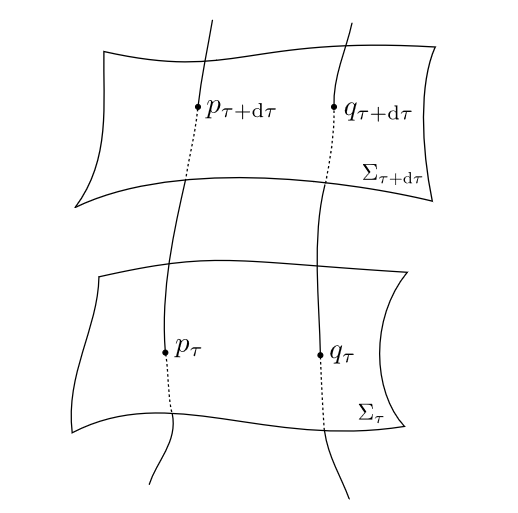
\includegraphics[scale=0.5]{immagini/osservatori_isotropi.png}
    \caption{Il tempo proprio permette di identificare le ipersuperfici di omogeneità. La differenza di tempo proprio misurata tra le due ipersuperfici dai due osservatori è la stessa.}
    \label{fig.osservatori_iso}
\end{figure}
La metrica in 4 dimensioni é:
\begin{equation}
    ds^2 = -d\tau^2 + a^2(\tau)d\Omega_k^2
    \label{eq.metrica_flrw}
\end{equation}
che viene detta \textbf{metrica di Friedmann-Lema\^itre-Robertson-Walker}, dove $k=0,\pm 1$ e $a(\tau)$ fattore di scala o anche detto parametro di scala dell'universo. L'elemento $d\Omega_k$ rappresenta lo spostamento sulla sottovarietà omogenea e isotropa tridimensionale. Si osserva che i termini $l$ che appaiono in eq. \ref{eq.metrica_s3}, \ref{eq.metrica_h3} sono assorbiti dal fattore $a$.
Questo non è determinato da ipotesi di simmetria come il resto della metrica, ma deve essere determinato inserendo la metrica nelle equazioni di Einstein eq. \ref{eq.GRequazioneeinstein}. Ovviamente in queste manca un aspetto che non si è ancora affrontato, ovvero quale sia il tensore di energia-impulso idoneo a descrivere l'universo.

\section{Galassie, polveri, radiazione ed energia oscura}\label{para.polveri}
Il primo elemento che va incluso per la descrizione dell'universo è la materia ordinaria e in particolare le galassie composte da essa. Le galassie possiamo assimilarle con buona approssimazione ad un \textbf{polvere} nel contesto cosmologico in quanto ciò può essere supportato da misure cosmiche. Con polvere si intende che questi elementi di materia ordinaria non possiedono pressione, $P=0$; le velocità casuali delle galassie sono piccole e ciò permette di trascurare la pressione di questa polvere di galassie.
All'interno di questo modello, il fluido cosmico sarà quindi idealizzato in un fluido perfetto, già descritto in \S\ref{para.fluido}:
\begin{equation*}
    T_{\mu\nu} = \rho u_\mu u_\nu
\end{equation*}
dove $\rho$ è la densità di massa media della materia e $u$ è il vettore tangente alle linee di mondo. Osserviamo infatti che le linee di mondo delle galassie devono coincidere con quelle degli osservatori isotropi in quanto il moto relativo tra questi può essere usato come direzione privilegiata. Proprio per via di questo moto relativo trascurabile, possiamo adottare come tensore energia-impulso quello del fluido perfetto relativistico.

Oltre alla materia ordinaria si considera anche la presenza della radiazione elettromagnetica con tensore energia-impulso:
\begin{equation*}
    T_{\mu\nu} = \frac{1}{4\pi} \left[ F_{\mu\alpha}\tensor{F}{^\alpha_\nu} - \frac{1}{4}g_{\mu\nu}F_{\alpha\beta}F^{\alpha\beta} \right]
\end{equation*}
è tensore a traccia nulla, $\tensor{T}{^\mu_\mu}=0$. Usando l'eq. \ref{eq.fluidoperfetto} del fluido perfetto e ponendo la traccia nulla, si ottiene l'equazione di stato per la radiazione:
\begin{equation*}
    P = \frac{\rho}{3}
\end{equation*}

L'energia-impulso nella forma di fluido perfetto che ci permette di descrivere l'universo è la fusione delle due ed è la forma più generale e compatibile con l'omogeneità e isotropia.
\begin{equation*}
    T_{\mu\nu} = \rho u_\mu u_\nu + P(g_{\mu\nu} +u_\mu u_\nu)
\end{equation*}

Normalmente ci si sarebbe fermati qui: considerata la radiazione e la materia ordinaria non ci dovrebbe essere null'altro. Purtroppo non è proprio così. Grazie ai loro lavori del 1998 \cite{1998_1} \cite{1998_2}, Saul Perlmutter, Brian P. Schmidt e Adam G. Riess (premi Nobel nel 2011), mostrarono attraverso l'osservazione del redshift di supernove l'espansione dell'universo e che questo stesse pure accelerando. Ulteriori osservazioni delle anisotropie della CMB, delle abbondanze degli elementi dovute alla nucleosintesi primordiale (elio in particolare), della struttura a grande scala dell'Universo, del clustering di galassie e delle misurazioni del parametro di Hubble hanno confermato l'espansione dell'universo nonché forniscono un importante confronto tra la teoria e le osservazioni. Il modello attualmente più soddisfacente per spiegare queste osservazioni prende il nome di $\Lambda$CDM (\emph{cold dark matter}). Chiaramente qui si vedrà la descrizione base.

Si è quindi introdotto il concetto di \textbf{energia oscura} per giustificare l'esistenza di una forza \emph{antigravitazionale} che giustificasse questa rapida espansione. Dagli studi sulla CMB, in particolare per mezzo del satellite WMAP, si è potuto stimare che l'universo fosse composto approssimativamente  da $\sim 5\%$ da materia ordinaria (barionica), $\sim 22\%$ da materia oscura (materia di natura sconosciuta, non osservabile tramite radiazione) e per il $\sim 73 \%$ da energia oscura. Questa energia oscura potrebbe essere rappresentata dalla \textbf{energia del vuoto}, concetto emerso dalla teoria quantistica dei campi che descrive l'energia dovuta alle cosiddette \emph{fluttuazioni del vuoto} ovvero alla continua annichilazione di coppie particella-antiparticella virtuali.

Il più semplice modello di energia oscura che tratteremo qui sarà basato sulla \textbf{costante cosmologica} $\Lambda$. Un aspetto fondamentale è che questa densità di energia associata alla costante è incredibilmente piccola per gli standard della fisica delle particelle; ciò rende complicato il legame con l'energia del vuoto, visto che tutti questi contributi energetici dovrebbero partecipare all'effettivo valore della costante. La natura dell'energia oscura, il suo legame con le altre branche della fisica e il valore della costante $\Lambda$ sono tutti problemi ancora aperti.

Nel 1917 Einstein riformulò le sue equazioni nella forma:
\begin{equation}
    G_{\mu\nu} + \Lambda g_{\mu\nu} = 8\pi T_{\mu\nu}
    \label{eq.GR_eqeinstein_cosmologica}
\end{equation}
per la descrizione di un primo modello cosmologico che descrivesse uno spazio di volume finito, ma illimitato\footnote{In una lettera a Willem de Sitter dello stesso anno scrisse che questo suo modello cosmologico fu sviluppato principalmente per vedere se \virgolette{l'idea base della relatività si potesse perseguire fino al suo completamento o se portasse a contraddizioni} e non tanto se il modello corrispondesse alle osservazioni.}. Il termine aggiuntivo fu introdotto per contrastare l'eventualità di un universo dinamico, che potesse contrarsi o espandersi, e ristabilire un universo statico, come per sua convinzione. Le soluzioni statiche per queste equazioni hanno tutt'al più la  caratteristica di essere instabili. Aggiungiamo inoltre che con un $\Lambda \neq 0$ non si può riottenere la teoria newtoniana, a meno che $\Lambda$ non sia sufficientemente piccola, così che le deviazioni dalla teoria di Newton non possano essere notate. 

Quando nel 1929 Hubble verificò l'espansione dell'universo\footnote{L'introduzione di $\Lambda$ fu considerata da Einstein stesso \emph{\virgolette{il mio più grande errore}}.}, la costante cosmologica cadde in disuso per poi riessere introdotta nel modello a energia oscura tramite le equazioni:
\begin{equation}
    G_{\mu\nu} = - \Lambda g_{\mu\nu}
    \label{eq.einstein_cosmologica_en_oscura}
\end{equation}

Interpretiamo dunque il termine cosmologico come un fluido perfetto:
\begin{equation*}
    - \Lambda g_{\mu\nu} = 8\pi T_{\mu\nu} = 8\pi( \rho u_\mu u_\nu + P(g_{\mu\nu} +u_\mu u_\nu))
\end{equation*}
per cancellare i termini $u_\mu u_\nu$ si deve porre:
\begin{equation*}
    P= - \rho
\end{equation*}
e questa è l'equazione di stato per l'energia oscura. Espressa in termini della costante cosmologica:
\begin{equation*}
    P = - \rho = - \frac{\Lambda}{8\pi}
\end{equation*}
Si osserva che con la costante cosmologica positiva, la pressione associata all'energia oscura è negativa.

\section{Equazioni di Friedmann e legge di Hubble}
Inserendo la metrica di FLRW, eq. \ref{eq.metrica_flrw}, nelle equazioni di Einstein:
\begin{equation*}
    G_{\mu\nu} = 8\pi T_{\mu\nu} = 8\pi( \rho u_\mu u_\nu + P(g_{\mu\nu} +u_\mu u_\nu))
\end{equation*}
si ottengono le equazioni:
\begin{equation}
    \left\{\begin{array}{l}
      \frac{\Dot{a}^2}{a^2} = \frac{8\pi}{3}\rho - \frac{k}{a^2} \\ \\
      \frac{3 \Ddot{a}}{a} = - 4\pi (\rho + 3P)
    \end{array}\right.
    \label{eq.equazioni_friedmann}
\end{equation}
dette \textbf{equazioni di Friedmann}. Le quantità incognite sono $a, \rho, P$ pertanto le equazioni di Friedmann devono essere accompagnate da un equazione di stato affinché si possa determinare una soluzione.

Se $\rho >0$ e $P \geq 0$ si ottiene, osservando la seconda equazione, che l'universo considerato non è più statico, ma in espansione o contrazione. Il termine $\Lambda$ fu qui introdotto da Einstein affinché $\rho -3P =0$ $(P<0)$ e quindi l'universo rimanesse statico.
\'E importante notare che quando si parla di espansione e contrazione dell'universo, la distanza tra gli osservatori isotropi (cioè le galassie) varia col tempo, ma non è presente alcun centro di espansione/contrazione; si può pensare ai punti disegnati sulla superficie di un palloncino quando lo si gonfia o sgonfia per esempio.

La domanda alla base della legge di Hubble che ora determineremo è capire quale sia questa velocità di espansione/contrazione. A tal fine consideriamo la metrica FLRW, eq. \ref{eq.metrica_flrw}, due osservatori con le loro linee di mondo perpendicolari alle due superfici di omogeneità $\Sigma$ in due tempi successivi $\tau, \tau + d\tau$; chiamiamo le distanze tra i due osservatori su queste ipersuperfici $R(\tau), R(\tau d\tau)$. Poichè sulle superfici $\tau$ è preso costante, si ha il termine $d\tau=0$ nella metrica.

Sulle ipersuperfici si calcola:
\begin{align*}
    R(\tau) &= \int ds = \int a(\tau)d\Omega = a(\tau) \int d\Omega \\
    R(\tau + d\tau) &= a(\tau +d\tau)\int d\Omega = a(\tau +d\tau) \frac{R(\tau)}{a(\tau)}
\end{align*}
Calcoliamo così la derivata:
\begin{align*}
    \frac{dR}{d\tau} &= \lim_{d\tau \rightarrow 0} \frac{   R(\tau + d\tau)-   R(\tau)}{d\tau} = \lim_{d\tau \rightarrow 0}  \frac{a(\tau +d\tau) \frac{R(\tau)}{a(\tau)} -  R(\tau)}{d\tau} \\
    &= \lim_{d\tau \rightarrow 0}  \frac{(a(\tau)+ \Dot{a}(\tau)d\tau) \frac{R(\tau)}{a(\tau)} -  R(\tau)}{d\tau} =\frac{\Dot{a}}{a} R
\end{align*}

Si ottiene quindi la \textbf{legge di Hubble}:
\begin{equation}
    v = \frac{\Dot{a}}{a} R
    \label{eq.legge_hubble}
\end{equation}
dove si definisce il \textbf{parametro di Hubble}:
\begin{equation*}
    H=  \frac{\Dot{a}}{a}
\end{equation*}

Nel 1929 Edwin Hubble e Milton Humason mostrarono che effettivamente le galassie più lontane si allontanassero dalla Terra, osservando il redshift delle stesse. Pertanto è confermato sperimentalmente che
\begin{equation*}
    \Dot{a} > 0
\end{equation*}
Tale risultato rappresenta un enorme successo della relatività generale.

Assumendo $\rho, P >0$ e $\Dot{a}>0$ si ha dalla seconda equazione di \ref{eq.equazioni_friedmann} che $\Ddot{a}<0$. Come conseguenza si può stimare superiormente l'età dell'universo visualizzando in un grafico la funzione $a(\tau)$ e la retta tangente al tempo proprio attuale: la distanza tra l'intersezione con l'asse delle ascisse e il tempo proprio attuale determina tale stima.
In particolare detto $\phi$ l'angolo con le ascisse si ricava:
\begin{equation*}
    \tan \phi = \frac{a(\tau)}{T}= \Dot{a}(T) \implies T= \frac{a}{\dot{a}} = H^{-1}
\end{equation*}
Quindi in tale stima, l'inverso della costante di Hubble fornisce l'età dell'universo, detto anche tempo di Hubble. Segue che la quantità $cH^{-1}$, chiamata lunghezza di Hubble, fornisce la stima del raggio dell'universo osservabile; questa è anche detta orizzonte cosmologico.

Inoltre un modello di espansione di questo tipo determina l'esistenza del cosiddetto \textbf{big bang} dove $a(\tau)=0$. In tale punto la distanza tra tutti i punto dello spazio è nulla, la curvatura e la densità di materia in questo stato sono infinite. Si potrebbe pensare di estendere l'universo oltre tale singolarità come svolto nell'espansione di Kruskal, tuttavia non è possibile in quanto questa è invece una singolarità di curvatura. Non ha pertanto senso chiedersi cosa fosse esistito prima o cosa ci sia \virgolette{oltre} al big bang\footnote{Nella teoria delle stringhe, dove sono introdotte 10 dimensioni, si è sviluppata invece una possibilità di descrivere come sia avvenuto il big bang.}. 
Si sottolinea infine che l'evoluzione dell'universo negli istanti appena successivi al big bang non può essere descritta da questa semplice trattazione (in tale periodo la densità di energia dominante era la radiazione a differenza di ora). 

\subsection{Universo statico di Einstein}
Investighiamo la soluzione statica ricercata da Einstein e accennata in \S\ref{para.polveri}, introdotta proprio a seguito dell'espansione/contrazione che si verifica con le \virgolette{normali} equazioni di Einstein, dove $\Lambda = 0$.

Imponiamo dunque che il fattore di scala sia costante $a = \textrm{cost.} = R$. La prima di Friedmann diventa:
\begin{equation*}
    R^2 = \frac{3k}{8\pi\rho}
\end{equation*}
affinché abbia senso, si distinguono le soluzioni con $\rho>0$, $k=1$ e $\rho<0$, $k=-1$. Investighiamo la prima nella quale si ha una densità di massa positiva e la geometria delle ipersuperfici è $S^3$.

La seconda di Friedmann diventa semplicemente:
\begin{equation*}
    P = - \frac{\rho}{3}
\end{equation*}
quindi negativa. Per la densità di massa consideriamo il contributo della costante cosmologica e della materia:
\begin{equation*}
    \rho = \rho_\Lambda + \rho_{mat.} = \frac{\Lambda}{8\pi} + \rho_{mat.}
\end{equation*}
La pressione risulta allora:
\begin{equation*}
    P = P_\Lambda = - \frac{\Lambda}{8\pi}
\end{equation*}
visto che il contributo della materia, assimilabile ad una polvere, determina $P=0$. Facendo queste sostituzioni nella seconda di Friedmann si ottiene la densità della materia:
\begin{equation*}
    \rho_{mat.} = 2\rho_\Lambda = \frac{\Lambda}{4\pi} \implies \rho = \frac{3\Lambda}{8\pi}
\end{equation*}
Quindi sostituendo la densità di massa totale nella prima Friedmann:
\begin{equation*}
    R^2 = \frac{1}{\Lambda} 
\end{equation*}

La metrica dell'universo statico di Einstein è quindi:
\begin{equation*}
    ds^2 = - d\tau^2 + \frac{1}{\Lambda}\left[ d\psi^2 + \sin^2\psi( d\theta^2 + \sin^2\theta d\phi^2)\right]
\end{equation*}
Tale universo presenta una topologia $\mathbb{R}\times S^3$; si era infatti detto che questo modello permetteva di descrivere uno spazio di volume finito, ma illimitato, proprio perché esso ha la struttura di una 3-sfera.

Una cosmologia di questo tipo è instabile; se $a < \frac{1}{\sqrt{\Lambda}}$ , anche di poco, allora $\rho_{mat.}$ è poco più grande di $2\rho_\Lambda$ e dalla seconda di eq. \ref{eq.equazioni_friedmann} di ottiene $\frac{\Ddot{a}}{a} < 0 $ e ciò porta $a$ a decrescere. Viceversa se $a > \frac{1}{\sqrt{\Lambda}}$, il fattore di scala inizia a crescere.
\section{Evoluzione della densità di massa}
Risolviamo a questo punto le equazioni di Friedmann per le diverse densità di energia. Riprendendo la prima equazione:
\begin{equation*}
    3\dot{a}^2 = 8\pi \rho a^2 -3k
\end{equation*}
Derivando
\begin{equation*}
    6\dot{a}\Ddot{a} = 16\pi \rho a \dot{a} + 8\pi \dot{\rho} a^2
\end{equation*}
Sostituendo la seconda di Friedmann in $\Ddot{a}$ e dividendo per $8\pi a^2$:
\begin{equation}
    \dot{\rho} + 3(\rho + P) \frac{\dot{a}}{a} = 0
    \label{eq.continuità_cosmologia}
\end{equation}
è l'equazione differenziale che determina l'evoluzione della densità di massa $\rho$ o anche detta equazione di continuità. Questa equazione può essere determinata calcolando direttamente $\nabla_\mu T^{\mu\nu} = 0$ ponendo $\nu = 0$. Come detto serve introdurre una equazione di stato che leghi $\rho, P$ e nel nostro caso si sceglie la generale equazione di stato lineare:
\begin{equation*}
    P = w \rho
\end{equation*}
dove
\begin{equation*}
    w = \left\{ \begin{array}{ll}
        0 & \textrm{galassie} \\
        1/3 & \textrm{radiazione} \\
        -1 & \textrm{energia oscura}
    \end{array}\right.
\end{equation*}

Osserviamo che esistono comunque modelli cosmologici, tipo il gas di Chaplygin che unifica energia oscura e materia oscura in un unico fluido, dove l'equazione non è lineare, ma ad esempio in tale caso $P \propto - \rho^{-2}$. Per valori $w < -1$, come le misurazioni attuali suggeriscono, la conseguenza ultima dell'universo è il \textbf{big rip}, ovvero un tempo finito nel quale tutte le distanze divergeranno.

Immettendo tale equazione di stato si ottiene:
\begin{equation*}
    \frac{\dot{\rho}}{\rho} + 3(1+w)\frac{\dot{a}}{a} = 0
\end{equation*}
che risolta:
\begin{equation*}
    \log \rho +3(1+w)\log a = \log C \implies \rho a^{3(1+w)} = c
\end{equation*}

Otteniamo dunque:
\begin{equation}
    \rho = ca^{-3(1+w)}
    \label{eq.evoluzione_densità_massa}
\end{equation}
che specializziamo:
\begin{itemize}
    \item Galassie, polveri
    \begin{equation*}
        \rho = c a^{-3}
    \end{equation*}
    
    La prima Friedmann diventa:
    \begin{equation*}
        3\frac{\dot{a}^2}{a^2} = 8\pi \rho -3\frac{k}{a^2} = 8\pi \frac{c}{a^3}-3 \frac{k}{a^2}
    \end{equation*}
    così che:
    \begin{equation*}
        \dot{a}^2 = \frac{c}{a}-k
    \end{equation*}
    dove $c=\frac{8\pi}{3}$. Risolta tramite separazione delle variabili ci porta alle soluzioni di tab. \ref{tab.galassie} e fig. \ref{fig.soluzioni_galassie}, nei vari casi di $k$:
    \begin{table}
        \centering
        \begin{tabular}{ccc}
        $k=1$ ($S^3$) & $k=0$ ($\mathbb{E}^3$) & $k=-1$ ($H^3$) \\
        \hline
        $a= \frac{c}{2}(1-\cos \eta)$     &  $a=(\frac{9c}{4})^{1/3}\tau^{2/3}$ &  $a= \frac{c}{2}(\cosh\eta-1)$ \\
        $\tau = \frac{c}{2}(\eta -\sin \eta)$ &     & $\tau = \frac{c}{2}(\sinh\eta - \eta)$ \\
        \hline
        \end{tabular}
        \caption{Soluzioni per le galassie.}
        \label{tab.galassie}
    \end{table}
    \begin{figure}
        \centering
        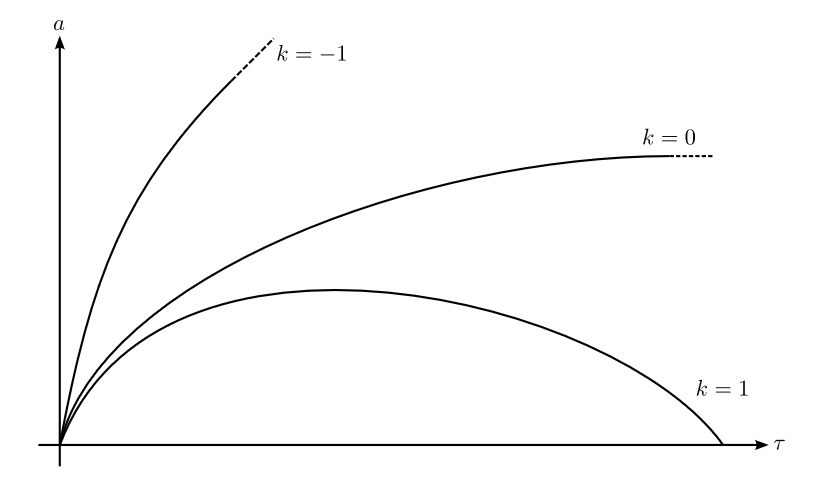
\includegraphics[scale=0.5]{immagini/soluzioni_galassie.png}
        \caption{Soluzioni alle equazioni di Friedmann per le galassie/polveri al variare di $k$.}
        \label{fig.soluzioni_galassie}
    \end{figure}
Le soluzioni corrispondenti a $k=-1,0$ sono tali da comportare un universo in espansione infinita; nel dettaglio si approcciano ad infinito con velocità $\dot{a}= 1, 0$ rispettivamente. La soluzione per $k=1$ invece comporta che l'universo sia in espansione fino a che $a=c$ $(\dot{a}=0)$ per poi contrarsi. Questa soluzione ha portato alla teoria del \textbf{big crunch}.

    \item Radiazione
    \begin{equation*}
        \rho = c a^{-4}
    \end{equation*}
    
    Si ottiene la prima di Friedmann:
    \begin{equation*}
        \dot{a}^2 - \frac{c'}{a^2} + k=0
    \end{equation*}
    dove $c'=\frac{8\pi}{3}$. Le soluzioni sono in tab. \ref{tab.radiazione}.
    \begin{table}
        \centering
        \begin{tabular}{ccc}
        $k=1$ ($S^3$) & $k=0$ ($\mathbb{E}^3$) & $k=-1$ ($H^3$) \\
        \hline
        $a= \sqrt{c'}\left( 1 - (1-\frac{\tau}{\sqrt{c'}})^2\right)^{1/2} $     &  $a= (4c')^{1/4}\tau^{1/2}$ &  $a= \sqrt{c'}\left((1+\frac{\tau}{\sqrt{c'}})^2 -1 \right)^{1/2}$ \\
        \hline
        \end{tabular}
        \caption{Soluzioni per la radiazione.}
        \label{tab.radiazione}
    \end{table}
    \item Energia oscura
    \begin{equation*}
        \rho = \textrm{cost.} = \frac{\Lambda}{8\pi}
    \end{equation*}
    
    La prima di Friedmann:
    \begin{equation*}
        3\frac{\dot{a}^2}{a^2}= \Lambda -3 \frac{k}{a^2}
    \end{equation*}
    ha le soluzioni di tab. \ref{tab.energiaoscura} e fig. \ref{fig.soluzioni_energia}.
    \begin{table}
        \centering
        \begin{tabular}{ccc}
        $k=1$ ($S^3$) & $k=0$ ($\mathbb{E}^3$) & $k=-1$ ($H^3$) \\
        \hline
        $a= \sqrt{\frac{3}{\Lambda}}\cosh \sqrt{\frac{\Lambda}{3}}\tau $     &  $a= e^{ \sqrt{\frac{\Lambda}{3}} \tau}$ &  $a=\sqrt{\frac{3}{\Lambda}}\sinh \sqrt{\frac{\Lambda}{3}}\tau $ \\
        \hline
        \end{tabular}
        \caption{Soluzioni per l'energia oscura.}
        \label{tab.energiaoscura}
    \end{table}
    \begin{figure}
        \centering
        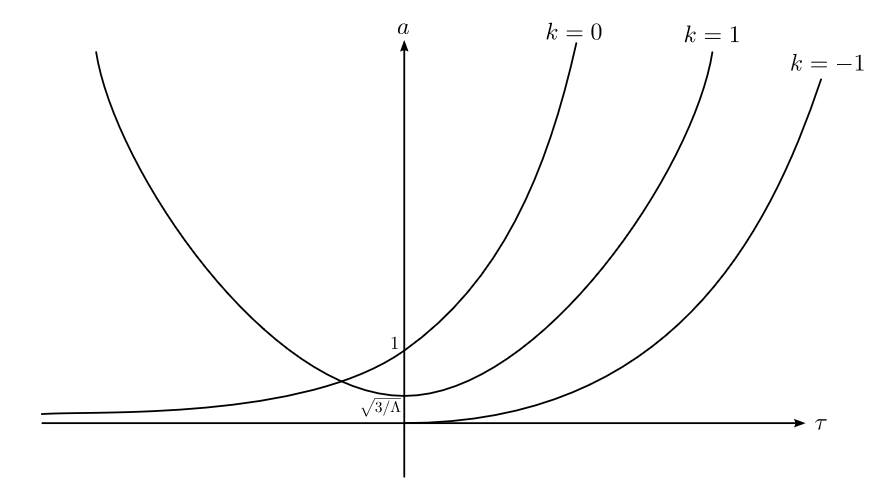
\includegraphics[scale=0.5]{immagini/soluzioni_energia.png}
        \caption{Soluzioni per l'energia oscura al variare di $k$.}
        \label{fig.soluzioni_energia}
    \end{figure}
    In questo caso le soluzioni sono isometriche e descrivono un universo detto \textbf{universo di de Sitter}. Un tale universo è privo di materia ordinaria e con costante cosmologica positiva che determina l'espansione dello stesso.
\end{itemize}

Osserviamo che per $a$ piccolo si ottiene che il termine dominante di $\rho$ è quello dovuto alla radiazione. Questo spiega come negli istanti successivi al big bang, l'universo fosse pervaso dalla radiazione, il cui contributo è andato ad affievolirsi per lasciare spazio ad un'era dominata dalla materia (anzi dall'energia oscura). Il contributo attuale della radiazione è dovuto alla CMB, come radiazione da corpo nero a $2.725$ K .

Al momento la metrica che descrive al meglio il nostro universo è:
\begin{equation}
    ds^2 = - d\tau^2 + e^{ 2\sqrt{\frac{\Lambda}{3}} \tau}( dx^2 + dy^2 + dz^2)
    \label{eq.metrica_universo}
\end{equation}
dove l'espansione dell'universo è esponenziale e lo spazio è a curvatura costante (spazialmente piatto). Un tale universo di de Sitter è detto in \textbf{coordinate inflazionarie}. Con inflazione cosmica si intende quella fase dopo al big bang, avvenuta intorno a $10^{-35} s$ dopo di esso e perdurata per $10^{30} s$, nella quale l'universo ha subito una drastica espansione accelerata, superiore a $10^{30}$ volte. Tale universo primordiale può essere descritto come universo di de Sitter.

Infine riassumiamo la classificazione dei vari spazi: un universo di de Sitter è l'analogo lorentziano ad uno spazio ellittico (la $n-$sfera), mentre un universo anti-de Sitter (corrispondente a $\Lambda <0$) è lo spazio lorentziano corrispondente allo spazio iperbolico. Lo spazio di Minkowski ($\Lambda = 0)$ è evidentemente l'analogo allo spazio euclideo.

\section{Equazioni di Friedmann in forma adimensionale}
Risulta particolarmente utile, soprattutto in ambito applicativo, riscrivere l'equazione di Friedmann (con le costanti esplicitate):
\begin{equation}
    H^2 = \frac{8\pi G}{3 c^2}\rho - \frac{kc^2}{ a^2}
\end{equation}
in termini di quantità adimensionali.  Si definiscono i parametri cosmologici:
\begin{equation}
    \Omega_w = \frac{\rho_{w,0}}{\rho_{crit, 0}}
\end{equation}
dove $w$ è lo stesso introdotto in precedenza e $\rho_{crit,0}$ è la densità critica ottenuta in un universo piatto, $k=0$, alla presente epoca, $H=H_0$:
\begin{equation}
    \rho_{crit,0} = \frac{3c^2}{8\pi G}H_0^2
\end{equation}
Dalla loro definizione, i parametri cosmologici descrivono la frazione di energia della componente $w$ osservata \textit{ad oggi}. 
I parametri sono definiti in modo tale che:
\begin{equation*}
    \sum_w \Omega_w = 1 + \frac{kc^2}{H_0^2}
\end{equation*}
\'E perciò possibile definire il parametro relativo alla curvatura $\Omega_k = - \frac{kc^2}{H_0^2}$. Sulla base di misure delle componenti di materia, radiazione e costante cosmologica nell'Universo, si può determinare il termine di curvatura $k$. Se la densità di energia totale risultasse, come le misure suggeriscono, $\Omega_0 + \Omega_\Lambda \approx 1$ allora l'Universo avrebbe una geometria quasi piatta. \'E bene notare che se $\Omega_k \neq 0$ allora non potrà mai essere veramente nulla e il suo valore evolverà nel tempo; il fatto che ora sia molto prossima a zero, implica che nell'Universo primordiale il suo valore fosse svariati ordini di grandezza ancora più vicina a zero ($o(10^{-16})$ alla nucleosintesi, $o(10^{-60})$ alla fine dell'inflazione). Questo \textit{fine tuning} prende il nome di \textbf{problema della piattezza}. 

L'equazione di Friedmann espressa con i parametri cosmologici diventa:
\begin{equation}
    \left(\frac{H}{H_0}\right)^2 = \frac{\Omega_r}{a^4} + \frac{\Omega_m}{a^3} + \frac{\Omega_k}{a^2} + \Omega_\Lambda
    \label{eq.friedmann_param_cosmologici}
\end{equation}
\section{Redshift cosmologico}
Consideriamo un osservatore, ad esempio una stella, che emette un fotone in $P_1$, il quale viene ricevuto da un secondo osservatore nel punto $P_2$ in un tempo proprio $\tau=\tau_2$. I punti $P_1, P_2$ sono punti delle ipersuperfici di omogeneità $\Sigma_\tau$ con $\tau = \tau_1, \tau_2$. Chiamiamo $u_i$ il relativo vettore ortogonale alla superficie e $\omega_i$ la frequenza emessa o ricevuta.
\begin{figure}
    \centering
    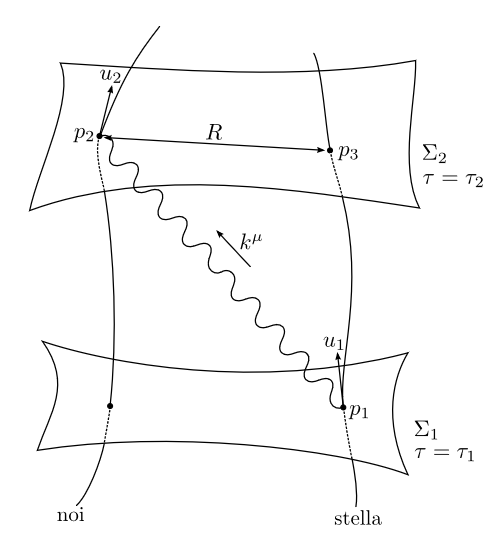
\includegraphics[scale=0.6]{immagini/redshiftcosmo.png}
    \caption{Redshift cosmologico}
    \label{fig.redshiftcosmo}
\end{figure}
Detto $k^\mu$ il vettore d'onda della luce, si avrà:
\begin{align*}
    \omega_1 = -k_\mu u_1^\mu && \omega_2 = - k_\mu u_2^\mu
\end{align*}

Vale in generale che si può trovare un vettore di Killing $\xi^\mu$ che punta nella direzione della proiezione di $k_\mu$ su $\Sigma_{\tau_1}$ in $P_1$, e similmente per $P_2$\footnote{Ad esempio per $k=0$, $\Sigma$ è piatta e possiamo assumere che $k_\mu$ proiettato su $\Sigma_{\tau_1}$ in $P_1$ sia nella direzione $\partial_x$ (altrimenti eseguiamo rotazione). Vale $<k,\partial_y> = < k, \partial_z> = 0$ al tempo iniziale; poiché $\partial_y, \partial_z$ sono di Killing e $k$ è tangente alla geodetica, questi prodotti scalari si conservano e rimangono tali lungo essa fino in $P_2$. Pertanto la proiezione di $k_\mu$ su $\Sigma_{\tau_2}$ in $P_2$ rimane lungo $\partial_x$ e $\xi =\partial_x$ è il vettore di Killing in questione. Ragionamento simile per $k=\pm 1$.}.

Inoltre dalla metrica, $ds^2 =  a^2(\tau)d\Omega^2$, si ha:
\begin{equation*}
    \frac{<\xi , \xi>^{1/2}|_{P_1}}{<\xi , \xi>^{1/2}|_{P_2}} = \frac{a(\tau_1)}{a(\tau_2)}
\end{equation*}
Scomponendo il vettore d'onda nelle componenti parallele e ortogonali all'ipersuperficie per il motivo prima detto:
\begin{equation*}
    k_\mu = A u_\mu + B \frac{\xi_\mu}{(\xi^2)^{1/2}}
\end{equation*}
dunque per la condizione $k_\mu k^\mu=0$ si avrà $A=B$ e dunque:
\begin{equation*}
    0 = A\left(  u_\mu k^\mu + \frac{\xi_\mu k^\mu}{(\xi^2)^{1/2}}\right) \iff - u_\mu k^\mu =  \frac{\xi_\mu k^\mu}{(\xi^2)^{1/2}}
\end{equation*}
ottenendo dunque:
\begin{equation*}
    \omega_{1,2} = \frac{\xi_\mu k^\mu}{(\xi^2)^{1/2}} \Big|_{P_{1,2}}
\end{equation*}

Facendo il rapporto si ottiene la relazione del \textbf{redshift cosmologico}:
\begin{equation}
    \frac{\omega_2}{\omega_1} =    \frac{<\xi , \xi>^{1/2}|_{P_1}}{<\xi , \xi>^{1/2}|_{P_2}} = \frac{a(\tau_1)}{a(\tau_2)}
    \label{eq.redshift_formale}
\end{equation}
dovuto all'espansione dell'universo, per la quale $a(\tau_1) \neq a(\tau_2)$.

Immaginiamo di essere l'osservatore $P_2$ e per convenienza richiamiamo $\tau_2 \rightarrow \tau_0$ ad indicare l'attuale tempo di osservazione, mentre $\tau_1 \rightarrow \tau_{em}$ per indicare quello di emissione del segnale, così siamo in una notazione più familiare. Utilizzando la convenzione usata in cosmologia dove il fattore di scala ad oggi è $a(\tau_0) = 1$, l'eq. \ref{eq.redshift_formale} diventa $\omega_{em}/\omega_{0} = a^{-1}(\tau_{em})$. Il redshift $z$ è definito:
\begin{equation}
    z = \frac{\omega_{em} - \omega_0}{\omega_0}
    \label{eq.redshift_z}
\end{equation}
e quindi si ottiene la relazione tra il fattore di scala e il redshift:
\begin{equation}
    a = (1+z)^{-1}
    \label{eq.redshift_relazione_a_z}
\end{equation}

Se differenziamo la formula del redshift $1+z = a(t_0)/a(t_{em})$, rispetto il tempo di osservazione $t_0$:
\begin{equation*}
    \frac{dz}{dt_0} = \frac{\Dot{a}(\tau_0)}{a(\tau_{em})} - \frac{a(\tau_0) \Dot{a(\tau_{em})}}{a^2(\tau_{em})}\frac{d\tau_{em}}{d\tau_0} = \left[H_0 - H(\tau_{em})\frac{d\tau_{em}}{d\tau_0} \right](1+z)
\end{equation*}
e richiamiamo il fatto che $\frac{d\tau_{em}}{d\tau_0} = \frac{1}{1+z}$ per gli stessi argomenti usati poco fa per definire il redshift, otteniamo:
\begin{equation*}
    \frac{dz}{d\tau_0} = H_0(1+z) - H(\tau_{em})
\end{equation*}
Con questa formula è possibile determinare la variazione del redshift col tempo o, viceversa, il valore del rate di espansione al tempo di emissione.
\section{Distanza di luminosità e diametro-angolare}
Per distanze cosmologiche dire che \virgolette{un oggetto è distante \textit{tot} anni-luce da noi} non è ben definito a meno di non fornire una definizione chiara del tipo di misura di distanza che si è effettuata. In particolar modo le misure di distanza che possiamo fare osservando il cielo sono legate al flusso di luce che ci giunge e alle dimensioni angolari degli oggetti.

Per quanto riguarda l'universo locale o semplicemente per nostra esperienza nella vita di tutti i giorni, oggetti con pari luminosità (intrinseche) posti a distanze differenti verranno osservati con luminosità (apparenti) diverse, minore per quello più distante. In uno spazio euclideo, la radiazione luminosa viene emessa isotropicamente e misurata con un flusso che scala con la superficie sferica di raggio pari alla distanza di osservazione $d$ secondo:
\begin{equation*}
    \Phi = \frac{L}{4\pi d^2}
\end{equation*}
Ovviamente una formula del genere è soggetta a possibili correzioni dovute all'assorbimento interstellare e/o intergalattico, che tuttavia trascuriamo ai nostri fini.
La quantità $L$ è la luminosità intrinseca dell'oggetto; tale valore può essere determinato per altre vie ad esempio utilizzando le cosiddette \emph{candele standard}, ovvero corpi per i quali possiamo risalire alla loro energia emessa in unità di tempo, dopo aver analizzato fenomeni \virgolette{standard} che avvengono all'interno di essi; sono un esempio le Cefeidi, stelle che variano le loro dimensioni con periodo proporzionale alla loro luminosità intrinseca, oppure le già citate supernove tipo 1A le quali posseggono una luminosità di picco comune al momento dell'esplosione.

Risulta abbastanza chiaro che quando si parla di distanze cosmologiche, dove i parametri cosmologici ed in particolare la geometria dello spaziotempo diventano rilevanti, tale formula deve essere cambiata. Determiniamo dunque la corretta formula nella cosmologia di FLRW.

Riscriviamo la metrica FLRW nella forma:
\begin{equation}
    ds^2 = -d\tau^2 +\left[ d\psi^2 + S_k(\psi)^2(d\theta^2 + \sin\theta^2 d\phi^2) \right]
    \label{eq.metrica_flrw_esplicitata}
\end{equation}
con
\begin{equation*}
    S_k(\psi) = \left\{ \begin{array}{cc}
        \sin\psi      & k= 1 \\
        \psi   & k= 0 \\
        \sinh\psi & k = -1 
    \end{array}\right.
\end{equation*}
Come conseguenza una sfera $S^2$ possiede ora una superficie di area $4\pi S_k^2(\psi)$. L'altro effetto da tenere in considerazione è quanto determinato nel paragrafo precedente ovvero il redshift delle luce dovuto alla distanza cosmologica. Un fotone emesso a frequenza $\nu_1$ giungerà all'osservatore con la frequenza (e quindi energia secondo l'equazione di Einstein-Planck):
\begin{equation*}
    \nu_0 = \frac{\nu_1}{1+z} \implies E_0 = \frac{E_1}{1+z}
\end{equation*}
dove $z$ è il redshift.
Con queste semplici considerazioni otteniamo che il flusso osservato ad una distanza comovente $\psi$ è:
\begin{equation}
    \Phi = \frac{L}{4\pi S_k(\psi)^2(1+z)^2}
    \label{eq.flusso_dist_cosmologica}
\end{equation}
Questo ci porta a definire la \textbf{distanza di luminosità}:
\begin{equation}
    d_L(\psi) =S_k(\psi)(1+z)
    \label{eq.luminosity_distance}
\end{equation}
Confrontando le due luminosità $L, \phi$ allora si ottiene che $d_L$ è una quantità effettivamente misurabile. Essa permette proprio la conversione tra luminosità intrinseca e apparente. Le tipiche distanze date in \virgolette{anni-luce} sono corrispondenti a $d_L$ che è monotona crescente con $z$.


Passando alla misura delle dimensioni angolari, come verrà mostrato, ci saranno importanti differenze rispetto il caso euclideo. La lunghezza d'arco $l$ di un oggetto è ottenuta dalla metrica FLRW di eq. \ref{eq.metrica_flrw_esplicitata} considerando $d\psi = d\phi =0$ a tempo fissato e integrando sull'angolo osservato:
\begin{equation*}
    l = \int ds = \int a(\tau_e)S_k(\psi)d\theta = a(\tau_e)S_k(\psi)\alpha
\end{equation*}
dove $\alpha$ è proprio l'angolo di estensione dell'oggetto; $\tau_e$ è il tempo di emissione del segnale e la relazione del redshift lega $a^{-1}(\tau_e) = 1+ z$. La \textbf{distanza diametro-angolare} è data dal rapporto tra la lunghezza d'arco $l$ e il rispettivo angolo $\alpha$ ed è pertanto:
\begin{equation}
    d_A(\psi) = \frac{S_k(\psi)}{1+z}
    \label{eq.distanza_diametro_angolare}
\end{equation}
Il suo utilizzo è quindi quello di convertire angoli in lunghezze fisiche trasverse $l = \alpha d_A$. In fig. \ref{fig.distanza_diametro_angolare_modelli} è mostrato come varia $d_A$ per alcuni modelli cosmologici. Si può notare che ad alto redshift $z>1$ le dimensioni angolari di un oggetto a $l=\cost$ aumentano invece che diminuire. Si potrebbe pensare che ciò porti al cosiddetto \textit{confusion limit} ovvero al fatto che gli oggetti cosmologici troppo lontani siano così grandi da sovrapporsi. Tuttavia questo non si verifica poiché le galassie ad alto redshift sono galassie giovani e quindi intrinsecamente piccole.
Si può anche notare che per determinati valori di $d_A$ vi corrispondono due ben differenti valori di $z$; questo corrisponde ad avere galassie con le stesse dimensioni angolari, ma di epoche e distanze ben differenti.
\begin{figure}[b]
    \centering
    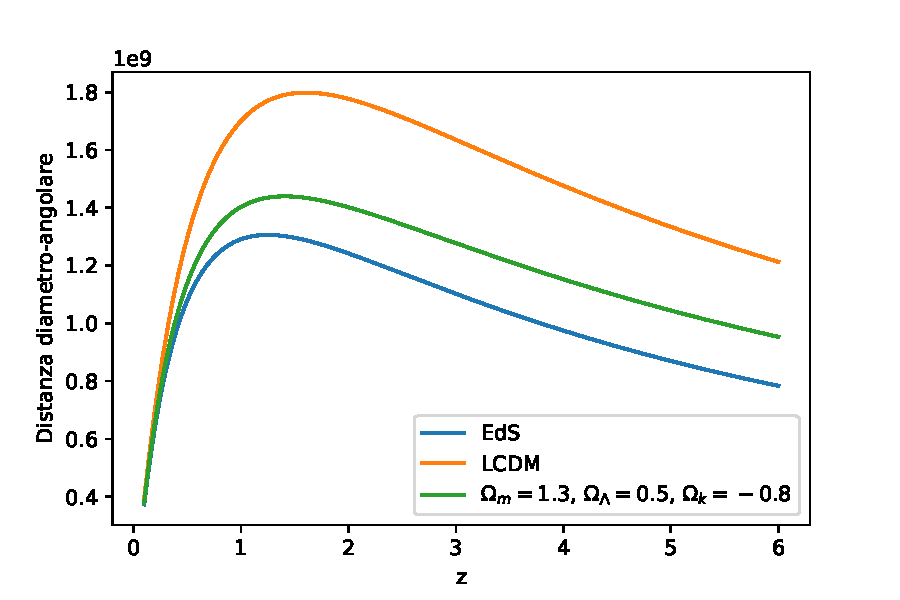
\includegraphics[scale=0.7]{immagini/distanza_diametro_angolare.pdf}
    \caption{Distanza diametro-angolare di eq. \ref{eq.distanza_diametro_angolare} in funzione del redshift $z$ in differenti modelli cosmologici. Einstein-de Sitter ($\Omega_m =1$), LCDM ($\Omega_m=0.3$, $\Omega_\Lambda = 0.7$, $\Omega_k= 0$) e un modello di materia chiuso. Si è usato $H_0 = 68 $ km/(Mpc s).}
    \label{fig.distanza_diametro_angolare_modelli}
\end{figure}

Se una sorgente luminosa ha una luminosità intrinseca per unità di area propria $\mathcal{L}$ allora per quanto visto, la sua luminosità apparente per una patch di area $A$ sarà $l = \mathcal L A/4\pi d_L^2$ e l'angolo solido sotteso da questa patch sarà $\Omega = A/d_A^2$. Pertanto si definisce la \textbf{brillanza superficiale} come la luminosità apparente per angolo solido:
\begin{equation}
    B = \frac{l}{\Omega} = \frac{\mathcal L d_A^2}{4\pi d_L^2} = (1+z)^{-4}\left( \frac{\mathcal L}{4\pi}\right)
    \label{eq.brillanza_superficiale}
\end{equation}
La quantità $(1+z)^{-4}$ è chiamata \textbf{cosmological dimming} ed è responsabile delle difficoltà legate all'osservazione ad alto redshift. La brillanza superficiale è stata utilizzata per verificare sperimentalmente che il fenomeno di redshift cosmologico fosse dovuto all'espansione dell'Universo e non a fenomeni di \textit{tired light}. Teorie di questo tipo prevedono l'Universo come statico e che i fotoni perdano la loro energia tramite meccanismi di differente natura. L'indipendenza tuttavia dalla misura diametro-angolare rende possibile l'esclusione di queste teorie per mezzo del test della brillanza superficiale. 
\chapter{Spazi a curvatura costante}\label{para.curvacost}
Nel precedente capitolo sulla cosmologia è stato mostrato come l'omogeneità e l'isotropia inducano sulle ipersuperfici di omogeneità una particolare forma del tensore di Riemann, eq. \ref{eq.riemann_curvatura_costante}, ed è stato detto che una varietà che abbia il Riemann che rispetti tale equazione sia detta a curvatura costante. Si è anche accennato alla catalogazione che posseggono gli spazi di dimensione $n$ con metrica di segnatura $n$, ovvero l'isometria con lo spazio iperbolico, euclideo e alla $n$-sfera a seconda del segno della costante $k$. Alla fine del capitolo è stata fornita una catalogazione analoga per gli spazi di metrica lorentziana, ovvero con lo spazio di Anti-de Sitter, di Minkowski e de Sitter, i quali dipendono invece dalla costante cosmologica.

In questo capitolo verranno affrontati nuovamente questi concetti in maniera più sistematica, mostrando per i vari spazi i principali sistemi di coordinate adottati.

\section{Spazio di Einstein}
Uno spazio a curvatura costante di dimensione $n$, ha il tensore di Riemann completamente determinato da:
\begin{equation*}
    R_{\mu\nu\rho\sigma} = \lambda ( g_{\nu\sigma}g_{\mu\rho}  - g_{\nu\rho}g_{\mu\sigma})
\end{equation*}
dove $\lambda= \textrm{cost.}$. Contraendo, seguono:
\begin{align*}
    R_{\nu\sigma} &= \lambda (n-1) g_{\nu\sigma} \\
    R &= \lambda n(n-1) \\
    G_{\nu\sigma} &= - \frac{1}{2}(n-1)(n-2) g_{\nu\sigma}
\end{align*}
Riprendendo le equazioni di Einstein, $G_{\nu\sigma} + \Lambda g_{\nu\sigma} = 0$, è possibile legare la costante di curvatura con la costante cosmologica:
\begin{equation*}
    \Lambda = \frac{(n-1)(n-2)}{2}\lambda = \frac{n-2}{2n}R
\end{equation*}

Si ricorda inoltre il teorema \ref{teo.killing} che determina che uno spazio a curvatura costante ha il numero massimo di vettori di Killing possibili.

\begin{definizione}
Una varietà che ha tensore di Einstein proporzionale alla metrica viene detto \textbf{spazio di Einstein}.
\end{definizione}
Alcuni testi matematici, vedi \cite{bruhat_manifolds}, riportano come definizione che il tensore di Ricci sia proporzionale alla metrica (del tutto equivalente).
Da questa definizione segue che:
\begin{equation*}
    \textrm{curvatura cost.} \implies \textrm{spazio di Einstein}
\end{equation*}
mentre in generale non è vero il viceversa, infatti lo spaziotempo di Schwarzschild ha $\Lambda = 0$, ma non è a curvatura costante. \'E però vero che in $n=3$ vale il viceversa, poiché in questo caso il tensore di Weyl, eq. \ref{eq.tensore_weyl}, è identicamente nullo e pertanto il tensore di Riemann dipende solamente dal tensore di Schouten secondo eq. \ref{eq.decomposizione_riemann_weyl}. A sua volta lo Schouten dipende dal Ricci e quindi dalla metrica, pertanto si ottiene uno spazio a curvatura costante. 

L'Universo di Einstein $\mathbb R \times S^3$ non è uno spazio di Einstein; una parte di esso è lo spazio di Minkowski che invece è spazio di Einstein con $\Lambda = 0$ (vedi pag. 122 di \cite{hawking}).
\section{Spazio di de Sitter}
Lo spazio di de Sitter è caratterizzato dal possedere $\Lambda > 0$. Esso viene determinato dall'immersione nello spazio di Minkowski $(d+1)$-dim.\footnote{Si esegue un procedimento analogo a quello per le metriche di $H^3$, $S^3$.} che chiamiamo $\mathbb{R}^{d+1}_1$, con coordinate $X^A$, $A = 0,1, \dots, d$, e metrica:
\begin{equation*}
    \eta_{AB} = diag(-1,1,\dots, 1)
\end{equation*}
\begin{equation*}
    ds^2 = - d(X^0)^2 + d(X^1)^2 + \dots + d(X^d)^2 
\end{equation*}

Chiamiamo lo spaziotempo di de Sitter $d$-dim. $dS_d$ corrispondente all'ipersuperficie:
\begin{equation*}
    \eta_{AB}X^A X^B = l^2
\end{equation*}
o esplicitamente:
\begin{equation*}
    -(X^0)^2 + (X^1)^2 + \dots + (X^d)^2 = l^2
\end{equation*}
per $X^0$ fissato, si hanno delle $(d-1)$-sfere di raggio $r = \sqrt{l^2 + (x^0)^2}$:
\begin{equation*}
    (X^1)^2 + \dots + (X^d)^2 = l^2 + (X^0)^2
\end{equation*}
pertanto lo spazio di de Sitter $dS_d$ sono delle $S^{d-1}$ a $X^0$ fissato che si contraggono ad un raggio minimo per poi espandersi, fig. \ref{fig.spazio_desitter}. La metrica su $dS_d$ è quella indotta da $\mathbb{R}^{d+1}_1$.
\'E uno spazio a curvatura costante positiva ed è quindi spazio di Einstein con tensore di Riemann:
\begin{equation*}
    R_{\mu\nu\rho\sigma} = \frac{1}{l^2}( g_{\nu\sigma}g_{\mu\rho}  - g_{\nu\rho}g_{\mu\sigma})
\end{equation*}

Il gruppo di isometrie per $dS_d$ è $O(d,1)$, in quanto sono le isometrie di $\mathbb{R}^{d+1}_1$ e quindi per la metrica indotta. Il gruppo ha il numero massimo di generatori $\frac{1}{2}d(d+1)$.

\begin{figure}
    \centering
    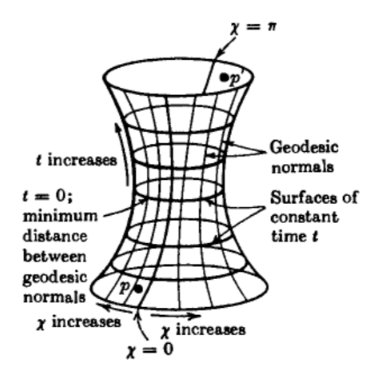
\includegraphics[scale=0.7]{immagini/spazio_desitter_embedding.png}
    \caption{Spazio di de Sitter $d$-dim. mostrato come immersione nello spazio di Minkowski $d+1$-dim.. Sono mostrate le coordinate globali che ricoprono l'intero iperboloide. Le superfici a $t = \textrm{cost.}$ sono $S^{d-1}$. }
    \label{fig.spazio_desitter}
\end{figure}
\subsection{Coordinate globali}
Ponendo $X^0 = l\sinh{\frac{\tau}{l}}$, si ottiene sostituendo:
\begin{equation*}
    (X^1)^2 + \dots + (X^d)^2 = l^2\cosh^2{\frac{\tau}{l}}
\end{equation*}
cioè delle $S^{d-1}$ con raggio $l\cosh{\frac{\tau}{l}}$. Si possono dunque introdurre delle coordinate sferiche nello spazio euclideo $\mathbb{R}^d$:
\begin{equation*}
    d(X^1)^2 + \dots + d(X^d)^2 = dr^2 + r^2d\Omega_{d-1}^2
\end{equation*}
dove $d\Omega_{d-1}^2$ è la metrica standard di $S^{d-1}$ di raggio 1. In questa maniera, usando il raggio precedente, si ottiene:
\begin{equation*}
        d(X^1)^2 + \dots + d(X^d)^2 = \sinh^2{\frac{\tau}{l}}dT^2 + l^2\cosh^2{\frac{\tau}{l}}d\Omega_{d-1}^2
\end{equation*}
e pertanto la metrica indotta su $dS_d$ nelle coordinate globali è:
\begin{equation}
    ds^2 = - d(X^0)^2 + d(X^1)^2 + \dots + d(X^d)^2 = - dT^2 + l^2\cosh^2{\frac{\tau}{l}}d\Omega_{d-1}^2
    \label{eq.desitter_globali}
\end{equation}
Sono coordinate che ricoprono l'intera varietà e la metrica è una forma di FLRW accelerante.

\subsection{Coordinate inflazionarie}
Utilizzando $(t, x^i)$ con $i= 1, \dots, d-1$ e $\bm{x}^2 = \sum_1^{d-1}x_i^2$, il sistema di coordinate è definito da:
\begin{align*}
    X^0 &= l\sinh\frac{t}{l} + \frac{\bm{x}^2}{2l}e^{t/l} \\
    X^i &= x^i e^{t/l} \\
    X^d &= l\cosh\frac{t}{l} - \frac{\bm{x}^2}{2l}e^{t/l}
\end{align*}
La metrica indotta risulta:
\begin{equation}
    ds^2 = \eta_{AB}dX^A dX^B = -dt^2 + e^{2t/l}d\bm{x}^2
    \label{eq.desitter_inflazionarie}
\end{equation}
dove $d\bm{x}^2$ è la metrica piatta $d-1$-dim..
Questa metrica è una forma di FLRW che ha le slice spaziali piatte, a coprire metà dello spazio $dS_d$.
\subsection{Coordinate statiche}
Le coordinate sono definite da:
\begin{equation*}
    (X^0)^2 - (X^d)^2 = r^2 - l^2
\end{equation*}
così che:
\begin{equation*}
    (X^1)^2 + \dots + (X^{d-1})^2 = r^2
\end{equation*}
corrispondente ad $S^{d-2}$. L'iperbole di $X^0$, $X^d$ può essere parametrizzata secondo:
\begin{align*}
    X^0 &= \sqrt{l^2 - r^2}\sinh \frac{t}{l} \\
    X^d &= \sqrt{l^2 - r^2}\cosh \frac{t}{l}
\end{align*}
con differenziali:
\begin{align*}
    dX^0 = -\frac{r}{\sqrt{l^2-r^2}}\sinh\frac{t}{l}dr &+ \frac{\sqrt{l^2-r^2}}{l}\cosh\frac{t}{l}dt \\
    dX^d = -\frac{r}{\sqrt{l^2-r^2}}\cosh\frac{t}{l}dr &+ \frac{\sqrt{l^2-r^2}}{l}\sinh\frac{t}{l}dt \\
    d(X^1)^2 + \dots + d(X^{d-1})^2 &= dr^2 + r^2 d\Omega_{d-2}^2
\end{align*}
La metrica indotta su $dS_d$ risulta:
\begin{equation}
    ds^2 = \eta_{AB}dX^A dX^B = - \left( 1 - \frac{r^2}{l^2} \right)dt^2 + \left(1 - \frac{r^2}{l^2}\right)^{-1}dr^2 + r^2 d\Omega_{d-2}^2
    \label{eq.metrica_desitter_statica}
\end{equation}

Questa metrica risulta simili a quella di Schwarzschild e presenta una singolarità delle coordinate in $r=l$ chiamata \textbf{orizzonte cosmologico}. Può solamente essere delle coordinate visto che negli altri sistemi di coordinate -- quello globale per primo -- non è presente.
\section{Spazio di Anti-de Sitter}
Consideriamo lo spazio $\mathbb{R}^{d+1}_2$ con coordinate $X^A$ dove $A = 0,\dots, d$ e metrica:
\begin{equation*}
    \eta_{AB} = diag(-1,1,\dots,1,-1)
\end{equation*}
Lo spaziotempo di Anti-de Sitter $AdS_d$ di dimensione $d$ è l'ipersuperficie:
\begin{equation*}
    \eta_{AB}X^A X^B = - l^2
\end{equation*}
Come gruppo di isometrie ha $O(d-1,2)$; il numero di generatori è massimo e pertanto è a curvatura costante (negativa).  La metrica indotta su $AdS_d$ ha il tensore di Riemann:
\begin{equation*}
    R_{\mu\nu\rho\sigma} = -\frac{1}{l^2}(g_{\nu\sigma}g_{\mu\rho} - g_{\nu\rho}g_{\mu\sigma})
\end{equation*}

Possiamo mostrare, ad esempio, $AdS_2$:
\begin{equation*}
    -(X^0)^2 + (X^1)^2 - (X^2)^2 = - l^2
\end{equation*}
dove per $X^1$ fissato si ottengono dei cerchi:
\begin{equation*}
       (X^0)^2 +  (X^2)^2 =  l^2 + (X^1)^2 
\end{equation*}
e lo spazio ha la forma mostrata in fig. \ref{fig.spazio_antidesitter}.
\begin{figure}
    \centering
    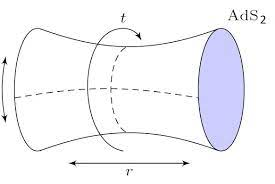
\includegraphics[scale=0.8]{immagini/spazio_antidesitter.jpeg}
    \caption{Topologia dello spazio $AdS_2$}
    \label{fig.spazio_antidesitter}
\end{figure}
\subsection{Coordinate globali}
Le coordinate globali su $AdS_d$ sono definite da:
\begin{equation*}
    (X^0)^2 + (X^d)^2 = r^2 + l^2 
\end{equation*}
dove:
\begin{equation*}
    (X^1)^2 + \dots + (X^{d-1})^2 = r^2
\end{equation*}
sono delle $S^{d-2}$ di raggio $r$. Il cerchio di $X^0$, $X^d$ può essere parametrizzato secondo:
\begin{align*}
    X^0 &= \sqrt{l^2 + r^2} \sin \frac{t}{l} \\
    X^d &= \sqrt{l^2 + r^2} \cos \frac{t}{l}
\end{align*}
La metrica indotta diventa:
\begin{equation}
    ds^2 = \eta_{AB}dX^a dX^B = - \left( 1 + \frac{r^2}{l^2}\right)dt^2 + \left( 1 + \frac{r^2}{l^2}\right)^{-1}dr^2 + r^2 d\Omega_{d-2}^2
    \label{eq.metrica_ads_statica}
\end{equation}
Questa metrica è simile alla metrica statica di $dS_d$, tuttavia non presenta più la singolarità per $r\rightarrow l$. \'E definita globalmente. Alcune volte questa metrica viene riscritta con il cambio di coordinate $r \mapsto l\sinh r$:
\begin{equation}
    ds^2 = -\cosh^2r dt^2 + l^2dr^2 + l^2\cosh^2r d\Omega_{d-2}^2
\end{equation}
\subsection{Coordinate di Poincarè}
Definendo le coordinate $(z, x^i,t)$ con $i = 1,\dots, d-2$ e $\bm{x}^2 = \sum (x^i)^2$,  legate secondo:
\begin{align*}
    X^0 &= \frac{z^2 + l^2 + \bm{x}^2 - t^2}{2z} \\
    X^i &= \frac{l}{z}x^i \\
    X^{d-1} &=  \frac{z^2 - l^2 + \bm{x}^2 - t^2}{2z} \\
    X^d &= \frac{l}{z}t
\end{align*}
La metrica indotta su $AdS_d$ diventa:
\begin{equation*}
    ds^2 = \eta_{AB}dX^A dX^B = \frac{l^2}{z^2}(- dt^2 + dz^2 + d\bm{x}^2)
\end{equation*}
Questa metrica è conformemente piatta.

Risulta utile mostrare il caso delle coordinate di Poincarè per $AdS_2$:
\begin{equation*}
    ds^2 = \frac{l^2}{z^2}(-dt^2 + dz^2)
\end{equation*}
se si esegue $z= \frac{l^2}{\rho}$ e si sostituisce si ottiene:
\begin{equation*}
    ds^2 = - \frac{\rho^2}{l^2}dt^2 + \frac{l^2}{\rho^2}d\rho^2
\end{equation*}
\subsection{Coordinate in forma FLRW}
Si esegue il cambio di coordinate secondo:
\begin{align*}
    X^0 &= l\sin\frac{\tau}{l} \\
    X^i &= l\cos\frac{\tau}{l}\sinh\rho x^i \\
    X^d &= l\cos\frac{\tau}{l}\cosh\rho
\end{align*}
così $\bm{x}^2 = \sum_1^{d-1} x^i = 1$ ovvero una $S^{d-2}$ di raggio 1. La metrica indotta su $AdS_d$ risulta:
\begin{equation*}
    ds^2 = - dT^2 + l^2\cos^2\frac{\tau}{l}(d\rho^2 + \sinh^2\rho d\Omega_{d-2}^2)
\end{equation*}
Le slice spaziali sono gli spazi iperbolici $H^{d-1}$. Osserviamo che si può avere in questa forma un \virgolette{big crunch} per $\tau/l = \frac{\pi}{2}$, ma è un artefatto delle coordinate poiché non viene osservato in quelle globali.
\section{Buchi neri immersi in AdS/dS}
Consideriamo la metrica:
\begin{equation}
    ds^2 = - \left( 1 - \frac{m}{r^{d-3}} + \frac{r^2}{l^2} \right)dt^2 + \left( 1 - \frac{m}{r^{d-3}} + \frac{r^2}{l^2} \right)^{-1}dr^2 + r^2d\Omega_{d-2}^2
    \label{eq.bh_in_ads}
\end{equation}
dove $m$ è un parametro di massa. Questa soluzione rappresenta uno spazio di Einstein senza però essere a curvatura costante. Si notano i casi limite:
\begin{itemize}
    \item $m=0 \implies AdS_d$
    \item $l\rightarrow + \infty \implies $ Schwarzschild in $d$-dim., detta  anche soluzione di \textbf{Schwarschild-Tangherlini}
\end{itemize}
I buchi neri immersi in $dS_d$ possono essere ottenuti dalla precedente metrica eseguendo la trasformazione $\frac{r^2}{l^2}\rightarrow - \frac{r^2}{l^2}$.

La metrica di eq. \ref{eq.bh_in_ads} può essere generalizzata, similmente a quanto effettuato per dedurre la soluzione di Schwarzschild, secondo:
\begin{equation}
    ds^2 = -\left( k - \frac{m}{r^{d-3}} + \frac{r^2}{l^2}  \right)dt^2 + \left( k - \frac{m}{r^{d-3}} + \frac{r^2}{l^2} \right)^{-1}dr^2 + r^2d\Sigma_{k, d-2}^2
    \label{eq.bhs_topolog_generaliz}
\end{equation}
dove $k = -1,0,1$ e $d\Sigma_{k,d-2}^2$ è, a seconda del valore $k$, la metrica su $H^{d-2}$, $\mathbb{E}^{d-2}, $$S^{d-2}$.
Questa generalizzazione risolve le equazioni di Einstein:
\begin{equation*}
    G_{\mu\nu} + \Lambda g_{\mu\nu} = 0
\end{equation*}
e ha orizzonte degli eventi nello zero più grande di $ k- \frac{m}{r^{d-3}} + \frac{r^2}{l^2} $. Nei casi $k=0, -1$ l'orizzonte non è compatto, ma può essere eseguita la compattificazione.
\begin{esempio}
Si considera $d = 4$ e $k=0$ in eq. \ref{eq.bhs_topolog_generaliz}. La compattificazione  viene eseguita tramite le coordinate di Hopf e l'immersione in $S^3$ che trasforma la metrica in:
\begin{equation*}
    ds^2 = d\alpha^2 + \cos^2\alpha d\phi^2 + \sin^2 \alpha d\psi^2
\end{equation*}
dove $\alpha \in [0,\frac{\pi}{2}]$, $ \phi \in [0,2\pi]$, $\psi \in [0, 2\pi]$.  Le sottovarietà a $\alpha = \textrm{cost.}$ sono un toro di Clifford, o toro piatto. Si parla infatti di buchi neri topologici in quanto posseggono un orizzonte dalla topologia non banale.
\end{esempio}
\chapter{Soluzioni di Kerr-Newman}
Nel capitolo \S\ref{para.schwarz} è stata vista la soluzione di Schwarzschild come prima, sia storicamente sia didatticamente, soluzione alle equazioni di campo di Einstein. In particolar modo la soluzione di Schwarzschild risulta l'unica soluzione che emerge dalle equazioni nel vuoto a simmetria sferica, come enunciato dal teorema di Birkhoff\footnote{Se è presente della carica, quindi si è in un sistema di equazioni di Einstein-Maxwell come fatto fra poco, allora la soluzione di Reissner-Nordstr\"om è l'unica sfericamente simmetrica.}.

Ulteriori soluzioni esatte alle equazioni di Einstein sono possibili e rientrano nella più generale metrica di Kerr-Newman. Per fare ciò sarà necessario alleggerire la richiesta di simmetria sferica, che come visto portava alla sola soluzione di Schwarzschild, per favorire l'assisimmetria. Il motivo per cui le soluzioni esatte siano trovate in spazi ad alta simmetria, è ovviamente dovuto alla complessità delle equazioni di Einstein.
Esistono teoremi di unicità per le soluzioni assisimmetriche, oltre a quello di Birkhoff.

\begin{definizione}
Uno spaziotempo asintoticamente piatto è \textbf{assisimmetrico} se esiste un campo vettoriale di Killing $m$ di tipo spazio vicino all'infinito spaziale e per cui tutte le orbite sono chiuse.

Si possono scegliere delle coordinate tali che $m = \partial_\phi$ è una coordinata di modulo $2\pi$.
\end{definizione}
\begin{teorema}[di Carter-Robinson]
Se $(\mathcal{M},g)$ è uno spaziotempo asintoticamente piatto, stazionario e assisimmetrico con $R_{\mu\nu} =0$ , non singolare fuori e sopra l'orizzonte, allora $(\mathcal{M}, g)$  è membro della famiglia di Kerr a due parametri $m$ (massa) e $J$ (momento angolare).
\end{teorema}

Questo teorema ci assicura l'esistenza della soluzione di Kerr.
La richiesta che lo spaziotempo sia assisimmetrico non è del tutto necessaria in quanto, per i buchi neri la stazionarietà implica l'assisimmetria.

Il teorema può essere ulteriormente generalizzato se si considera un sistema di equazioni di Einstein- Maxwell, quindi soddisfacenti l'azione eq. \ref{eq.azione_einstein_maxwell} che produce le equazioni del moto eq. \ref{eq.equazioni_einstein_maxwell}. 
In tal caso i buchi neri asintoticamente piatti e stazionari devono appartenere alla famiglia di Kerr-Newman a 3 parametri\footnote{Questo teorema viene chiamato \textit{no-hair theorem}. Jacob Bekenstein coniò questo nome dicendo che \virgolette{black holes have no hair} per esprimere un caratteristica dei buchi neri tutt'altro che banale:  tutte le proprietà che possiede la materia che componeva stelle collassate in buchi neri (campi magnetici, correnti di materia, rotazioni differenziali, inomogeneità) o particelle che accrescono quelli già esistenti (spin, numero leptonico o barionico) scompaiono una volta attraversato l'orizzonte degli eventi, nel senso che diventano permanentemente inaccessibili agli osservatori all'esterno, i quali riescono a descrivere il buco nero con solo questi tre parametri. Wheeler riportò in un'intervista che secondo Feynman la frase usata da Bekenstein fosse oscena e non volesse usarla.} (o 4 se consideriamo le cariche separate):
\begin{align}
    ds^2 &= - \frac{\Delta - a^2\sin^2\theta}{\rho^2}dt^2 - 2a\sin^2\theta\frac{r^2+a^2- \Delta}{\rho^2}dtd\phi + \nonumber \\
    & + \frac{(r^2+a^2)^2 - \Delta a^2\sin^2\theta}{\rho^2}\sin^2\theta d\phi^2 + \frac{\rho^2}{\Delta}dr^2 + \rho^2 d\theta^2
    \label{eq.metrica_kerr_newman}
\end{align}
dove:
\begin{align*}
    \rho^2 &= r^2 +a^2\cos^2\theta \\
    \Delta &= r^2 -2mr + a^2 + e^2
\end{align*}
metrica  che è accoppiata alla Maxwell 1-forma:
\begin{equation}
    A^2 = \frac{1}{\rho^2}\left[Qr(dt - a\sin^2\theta d\phi) - P\cos\theta[ adt - (r^2+a^2)d\phi] \right]
    \label{eq.maxwell_1forma}
\end{equation}
I parametri $a$, $m$ sono rispettivamente parametri di rotazione e massa, mentre $Q$, $P$ sono carica elettrica e magnetica che definiscono il terzo parametro:
\begin{equation*}
    e^2 = Q^2 + P^2
\end{equation*}
Può essere mostrato che il parametro di rotazione è collegato al momento angolare totale $J$ secondo:
\begin{equation*}
    a = \frac{J}{m}
\end{equation*}
Il sistema di coordinate $(t,r,\phi,\theta)$ che descrive la metrica eq. \ref{eq.metrica_kerr_newman} è chiamato di \textbf{Boyer-Lindquist}.

Si possono notare i seguenti casi limite:
\begin{itemize}
    \item $a = e = 0$ è la soluzione di Schwarzschild (non rotante, non carico, sfericamente simmetrico, statico).
    \item $a = 0$ è la soluzione di Reissner-Nordstr\"om (non rotante, carico, sfericamente simmetrico, statico).
    \item $e=0$ è la soluzione di Kerr (rotante, non carico, assisimmetrico, stazionario).
\end{itemize}
\section{Soluzione di Reissner-Nordstr\"om}
Questa soluzione permette di descrivere lo spazio esterno ad un corpo a simmetria sferica, carico e permette di generalizzare la soluzione di Schwarzschild. La metrica è:
\begin{equation}
    ds^2 = - \left(1 - \frac{2M}{r} + \frac{e^2}{r^2}\right)dt^2 + \frac{dr^2}{1 - \frac{2M}{r} + \frac{e^2}{r^2}} + r^2(d\theta^2 + \sin^2\theta d\phi^2)
    \label{eq.metrica_rn}
\end{equation}
e la Maxwell 1-forma\footnote{Può anche essere letta come $A^\mu = (\frac{Q}{r},0,0,P\cos\theta)$.}:
\begin{equation*}
    A = \frac{Q}{r}dt + P\cos \theta d\phi
\end{equation*}
L'orizzonte è determinato dalla singolarità delle coordinate, corrispondente ai valori:
\begin{equation*}
  r_{\pm} = M \pm \sqrt{M^2 - e^2}  
\end{equation*}
dove $r_+$ è detto orizzonte degli eventi, mentre $r_-$ è l'orizzonte di Cauchy. 
Poiché questi valori possono essere complessi, si ha un limite superiore alle cariche affinché possa essere ottenuto un buco nero:
\begin{equation*}
    P^2 + Q^2 \leq M^2
\end{equation*}
Per $e^2 > M^2$ non ci sono orizzonti e la singolarità è nuda. Il caso $r_+ = r_-$ è detto buco nero estremale.

\subsection{Buco nero estremale, soluzione di Bertotti-Robinson e di Majumdar-Papapetrou}
La metrica eq. \ref{eq.metrica_rn} diventa per $M=e$:
\begin{equation*}
    ds^2 = - \left(1 - \frac{e}{r} \right)^2dt^2 + \left(1 - \frac{e}{r} \right)^{-2}dr^2 + r^2 d\Omega^2
\end{equation*}
Introducendo la coordinata radiale:
\begin{equation*}
    \rho = r - e
\end{equation*}
detta \textbf{coordinata isotropa}, l'orizzonte viene portato al valore $\rho = 0$. Dunque la metrica diventa:
\begin{equation}
    ds^2 = - \left( 1 + \frac{e}{\rho}\right)^{-2}dt^2 +  \left( 1 + \frac{e}{\rho}\right)^2\left[ d\rho^2 + \rho^2 d\Omega^2\right]
    \label{eq.metrica_rn_estremale_isot}
\end{equation}
Si può far notare che la funzione $1 + \frac{e}{\rho}$ sia una funzione armonica di $\mathbb{E}^3$.
Studiamo la geometria vicino all'orizzonte: approssimiamo per $\rho \rightarrow 0$, $1 + \frac{e}{\rho} \simeq \frac{e}{\rho}$ così:
\begin{equation*}
    ds^2 = - \frac{\rho^2}{e^2}dt^2 + \frac{e^2}{\rho^2}d\rho^2 + e^2 d\Omega^2
\end{equation*}
In questa metrica si può riconoscere che la geometria è lo spazio prodotto $AdS_2 \times S^2$ , dove Anti-de Sitter è scritto in coordinate di Poincarè, mentre la 2-sfera ha raggio pari a $e$. Questa soluzione vicino all'orizzonte è detta \textbf{di Bertotti-Robinson}. Il gruppo di isometrie vicino all'orizzonte viene allargato da $\mathbb{R}\times SO(3)$ a $O(2,1)\times SO(3)$.

\'E possibile generalizzare la metrica e il potenziale di gauge $A$ a:
\begin{equation*}
        ds^2 = - V(\bm{x})^{-2}dt^2 + V(\bm{x})^2 d\bm{x}^2
\end{equation*}
\begin{equation*}
        A = V(\bm{x})^{-1}dt
\end{equation*}
dove, affinché siano soddisfatte le equazioni di Einstein:
\begin{equation*}
    \nabla^2_{\mathbb{E}^3} V(\bm{x}) = 0
\end{equation*}
Questa viene detta \textbf{soluzione di Majumdar-Papapetrou}.

Un caso particolare è dato dalla funzione armonica:
\begin{equation*}
    V(\bm{x}) = 1 + \sum_{i=1}^N \frac{M_i}{|\bm{x} - \bm{x}_i|}
\end{equation*}
corrispondente ad una configurazione di $N$ buchi neri di massa $M_i$ posti in $\bm{x}_i$.
Questo rappresenta un principio di sovrapposizione nella relatività generale che, data la natura fortemente non lineare delle equazioni di Einstein, non è fatto per nulla scontato. Ciò è possibile perché vi è un esatto bilancio tra le forze di attrazione gravitazionale con la repulsione elettrostatica. Dunque è solo possibile nel caso estremale.

\section{Soluzione di Kerr}
A differenza della soluzione di Schwarzschild, scoperta poco dopo la pubblicazione della relatività generale e la sua estensione carica con la metrica di Reissner-Nordstr\"om, ricavata sempre in quegli anni, ci sono voluti una cinquantina di anni per ottenere, nel 1963 grazie a R. Kerr, una metrica che descrivesse lo spaziotempo generato da un corpo non carico e rotante.
Ad oggi la metrica viene ricavata dalla più generale famiglia di Kerr-Newman, eq. \ref{eq.metrica_kerr_newman}, imponendo $e = 0$:
\begin{align}
ds^2 &= - \frac{\Delta - a^2\sin^2\theta}{\rho^2}dt^2 - 2a\sin^2\theta\frac{2mr}{\rho^2}dtd\phi + \nonumber \\
&+ \frac{(r^2 + a^2)^2- \Delta a^2\sin^2\theta}{\rho^2}\sin^2\theta d\phi^2 + \frac{\rho^2}{\Delta}dr^2 + \rho^2 d\theta^2
    \label{eq.metrica_kerr}
\end{align}
dove $\Delta = r^2 -2mr + a^2$ e $\rho^2 = r^2 + a^2\cos^2\theta$. Questa metrica è particolarmente importante dal punto di vista astrofisico, in quanto permette di descrivere le stelle rotanti a grandi distanze e i buchi neri astrofisici, che si osservano non possedere carica.  Il termine $g_{tt}$ può essere anche scritto nella forma:
\begin{equation*}
    g_{tt}= -\left( 1 - \frac{2M}{\rho^2}\right)
\end{equation*}
La soluzione di Kerr è una soluzione esatta alle equazioni di Einstein per $r > R$, con $R$ il raggio del corpo; non è stata accoppiata a nessuna soluzione che rappresenti l'interno di una stella, a differenza di Schwarzschild che, grazie al teorema di Birkhoff, descrive lo spaziotempo esterno esatto che si accoppia ad una soluzione interna sfericamente simmetrica\footnote{In \cite{tong} viene fatto notare che i teoremi di unicità come Carter-Robinson fanno uso esplicito dell'orizzonte degli eventi, mentre per Birkhoff l'unica assunzione è la simmetria sferica. Questo causa quanto appena detto. Inoltre rende la soluzione di Kerr valida come approssimazione a grandi distanze dalla superficie della stella.} .

La metrica di Kerr nel limite $M\rightarrow 0$ con $a$ fissato, si riduce alla metrica di Minkowski. Infatti ha la forma:
\begin{equation*}
    ds^2 = -dt^2 + \frac{r^2 + a^2\cos^2\theta}{r^2 + a^2}dr^2 + (r^2+a^2)\sin^2\theta d\phi^2 + (r^2 + a^2\cos^2\theta)d\theta^2
\end{equation*}
che con la trasformazione di coordinate:
\begin{equation*}
    \left\{ \begin{array}{l}
        \rho = \sqrt{r^2 + a^2}\sin\theta \\
        z = r\cos\theta          
    \end{array}\right.
\end{equation*}
i riduce a Minkowski in coordinate cilindriche, $ds^2 = -dt^2 + d\rho^2 +\rho^2 d\phi^2 + dz^2$.

La metrica di Kerr presenta due isometrie continue con i vettori di Killing che in opportune coordinate possono essere scritti (attenzione a non confondere il vettore di Killing $m$ con la massa):
\begin{equation*}
    k = \partial_t \qquad m =\partial_\phi
\end{equation*}
Kerr nella forma di Boyer-Lindquist, presenta una singolarità delle coordinate per $\Delta = (r - r_-)(r-r_+) = 0$ dove:
\begin{equation*}
    r_\pm = m \pm \sqrt{ m^2 - a^2}
\end{equation*}
Questa metrica è invariante sotto inversione simultanea di $t$ e $\phi$, mentre non lo è per la sola inversione temporale (a meno che $a=0$, ma è Schwarzschild): infatti l'inversione del tempo di un oggetto rotante determina l'oggetto in rotazione nel senso opposto.

Si distinguono 3 casi:

\subsubsection{$m^2 < a^2$} 
In questo caso $r_\pm \in \mathbb{C}$ e pertanto non c'è alcuna singolarità delle coordinate, solo quella di curvatura in $\rho = 0$ che corrisponde a $r= 0$ all'equatore $\theta = \frac{\pi}{2}$. Si verifica che è proprio di curvatura calcolando uno scalare di curvatura, come ad esempio $R_{\mu\nu\rho\sigma}R^{\mu\nu\rho\sigma}$.

La natura di questa singolarità può essere studiata nelle \textbf{coordinate di Kerr-Schild} definite secondo:
\begin{align*}
    x + iy &= (r + ia)\sin\theta e^{i \int ( d\phi + \frac{a}{\Delta}dr)} \\
    z &= r\cos\theta \\
    \Tilde{t} &= \int ( dt + \frac{r^2 + a^2}{\Delta}dr) -r
\end{align*}
che implica che  $r = r(x,y,z)$ sia dato implicitamente da:
\begin{equation*}
    r^4 - (x^2 + y^2 + z^2 - a^2)r^2 - a^2z^2 = 0
\end{equation*}
La metrica in queste coordinate è:
\begin{align}
    ds^2 &= - d\Tilde{t}^2 + dx^2 + dy^2 + dz^2 + \nonumber \\
 &+\frac{2mr^3}{r^4+a^2z^2}\left[ \frac{r(xdx + ydy) - a(xdy -ydx)}{r^2 + a^2} + \frac{zdz}{r} + d\Tilde{t}\right]^2
\label{eq.metrica_kerr_schild}
\end{align}
Si può notare che lo spaziotempo è piatto di Minkowski quando $m=0$.  Infatti per le coordinate di Kerr-Schild vale sempre la scrittura\footnote{Esistono anche i \textit{double Kerr-Schild} per i quali vale $g_{\mu\nu} = \eta_{\mu\nu} + k_\mu k_\nu + l_\mu l_\nu$}:
\begin{equation}
    g_{\mu\nu} = \eta_{\mu\nu} + k_\mu k_\nu
\end{equation}

Si può osservare che le superfici $r=\textrm{cost.}$, $\Tilde{t}= \textrm{cost.}$ sono ellissoidi confocali che degenerano in $r= 0$ al disco:
\begin{align*}
    z = 0 && x^2 + y^2 \leq a^2
\end{align*}
ovvero:
\begin{equation*}
    (x+iy)(x-iy) = (r^2 + a^2)\sin^2\theta \leq r^2 + a^2
\end{equation*}
La singolarità di curvatura ottenuta a $\theta = \frac{\pi}{2}$ corrisponde al bordo del disco $z = 0$, $x^2 +y^2 = a^2$ e viene detta \textbf{ring singularity}.

Inoltre, a differenza di Schwarzschild, non c'è motivo di restringere $r$ ai soli valori positivi, pertanto lo spaziotempo può essere continuato analiticamente attraverso il disco ad un'altra regione asintoticamente piatta dove però $r < 0$.

Possiamo inoltre mostrare la struttura causale di questa soluzione. Poiché Kerr gode di simmetria assiale e non sferica, sarebbe necessario un diagramma 3d per le coordinate $(t,r,\theta)$; tuttavia possiamo restringerci alle sottovarietà $\theta = 0$ e $\theta = \frac{\pi}{2}$ in quanto queste sono \textbf{totalgeodetiche}, ovvero le geodetiche delle sottovarietà lo sono per la varietà stessa o in altre parole le geodetiche inizialmente tangenti alla sottovarietà, rimangono tangenti alla sottovarietà.
In fig. \ref{fig.kerr_causale_1}
\begin{figure}
    \centering
    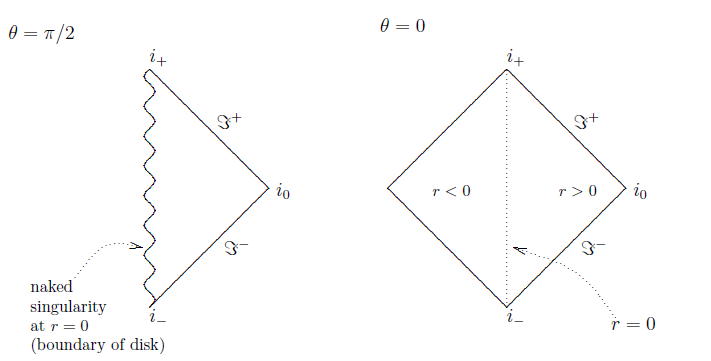
\includegraphics[scale=0.7]{immagini/kerr_causale_1.png}
    \caption{Struttura causale per Kerr con $m^2 < a^2$ per la sottovarietà equatoriale $\theta = \frac{\pi}{2}$ e per lungo l'asse $\theta = 0$. Nel primo caso, la geodetica nulla radiale e ingoing colpisce la ring singularity a $r=0$: la singolarità è nuda. Nel secondo caso le stesse geodetiche lungo l'asse di simmetria attraversano il disco in $r=0$ e finiscono in $r<0$.}
    \label{fig.kerr_causale_1}
\end{figure}
Il motivo principale per cui questo spaziotempo non è fisico è dovuto al vettore di Killing $\partial_\phi$ che diventa di tipo tempo in $r<0$, vicino alla ring singularity. Ciò determina un comportamento non causale in quanto le orbite di $\partial_\phi$ sono chiuse. Nel dettaglio:
\begin{equation*}
    \partial^2_\phi = g_{\phi\phi} = a^2\sin^2\theta \left( 1 + \frac{r^2}{a^2}\right) + \frac{ma^2}{r}\left( \frac{2\sin^4\theta}{1 + \frac{a^2}{r^2}\cos^2\theta}\right) 
\end{equation*}
Quando $r/a = \delta \ll 1$ e considerando $\theta = \pi/2 + \delta$ si ha allora:
\begin{equation*}
    \partial^2_\phi = a^2 + \frac{Ma}{\delta} + o(\delta) < 0
\end{equation*}
quando $\delta$ è sufficientemente piccolo e negativo (vicino $r<0$).
\subsubsection{$m^2 > a^2$}
In questo caso c'è una ring singularity, ma la metrica ha singolarità delle coordinate in $r_\pm$ con Boyer-Lindquist. Per questo motivo si introducono le \textbf{coordinate di Kerr}:
\begin{align*}
    dv &= dt + \frac{r^2 + a^2}{\Delta} dr\\
    d\chi &= d\phi + \frac{a}{\Delta}dr
\end{align*}
e la metrica diventa:
\begin{align}
    ds^2 &= - \frac{\Delta - a^2\sin^2\theta}{\rho^2}dv^2 + 2dvdr - \frac{2a\sin^2\theta(r^2 + a^2 - \Delta)}{\rho^2}dvd\chi + \nonumber \\ &- 2a\sin^2\theta d\chi dr + \frac{(r^2 + a^2)^2 - \Delta a^2\sin^2\theta}{\rho^2}\sin^2\theta d\chi^2 + \rho^2 d\theta^2
\label{eq.metrica_kerr_coord_kerr}
\end{align}

Si può mostrare che le ipersuperfici $r = r_\pm$ sono orizzonti di Killing per i vettori di Killing:
\begin{equation*}
    \xi_\pm = \partial_t + \frac{a}{r^2_\pm + a^2} \partial_\phi
\end{equation*}
E la rispettiva gravità superficiale è:
\begin{equation}
    \kappa_\pm =\frac{r_\pm - r_\mp}{2(r^2_\pm + a^2)}
\label{eq.grav_sup_kerr}
\end{equation}
La struttura causale è mostrata in fig. \ref{fig.kerr_causale_2}.
L'orizzonte degli eventi è a sua volta un orizzonte di Killing di:
\begin{equation*}
    \xi = \partial_t + \Omega_H \partial_\phi
\end{equation*}
con
\begin{equation}
    \Omega_H = \frac{a}{r^2_+ + a^2}
    \label{eq.omega_kerr}
\end{equation}
Segue che se applichiamo $\xi$ a $\phi - \Omega_H t$,:
\begin{equation*}
    \xi(\phi - \Omega_H t) = (\partial_t + \Omega_H \partial_\phi) (\phi - \Omega_H t) = - \Omega_H + \Omega_H = 0
\end{equation*}
Pertanto $\phi = \Omega_H t + \textrm{cost.}$ sulle orbite di $\xi$; allo stesso tempo $\phi = \textrm{cost.}$ sulle orbite di $\partial_t$. Queste informazioni ci permettono di affermare che le particelle su orbite di $\xi$ ruotano con velocità angolare $\Omega_H$ relativa a quelle statiche, su orbite di $\partial_t$, e quindi rispetto un sistema di riferimento stazionario posto all'infinito.
I generatori nulli dell'orizzonte seguono orbite di $\xi$ e ciò ci fa dire che il buco nero di Kerr ruota con velocità angolare $\Omega_H$.
\begin{figure}
    \centering
    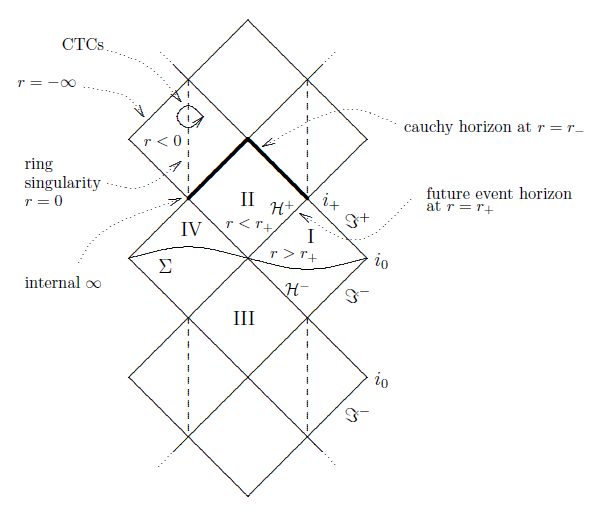
\includegraphics[scale=0.7]{immagini/kerr_causale_2.png}
    \caption{Struttura causale di Kerr $m^2 > a^2$ per $\theta = 0$. Il grafico può essere esteso in entrambe le direzioni (CTCs sta per \textit{closed timelike curves}).}
    \label{fig.kerr_causale_2}
\end{figure}
\subsubsection{$m^2 = a^2$}
Il buco nero di Kerr è estremo. Segue che $r_+=r_-= m$ e le gravità superficiali $\kappa_+ = \kappa_- = 0$; la temperatura di Hawking è pertanto nulla. L'orizzonte di Killing a $r = m$ è degenere ($\kappa =0)$ per il campo di Killing:
\begin{equation*}
    \xi = \partial_t + \Omega_H \partial_\phi \ \textrm{ con } \ \Omega_H = \frac{a}{2m}
\end{equation*}
Il diagramma di Penrose per questo caso è mostrato in fig. \ref{fig.kerr_causale_3}.
Si nota comunque che, nonostante possano esistere angoli $\theta$ per i quali possa avvenire il passaggio a $r<0$ attraverso $r=0$, questo fisicamente non si verifica in quanto nel collasso gravitazionale delle stelle non si verificano le condizioni per le quali questo \virgolette{ponte} sia attraversabile.
\begin{figure}
    \centering
    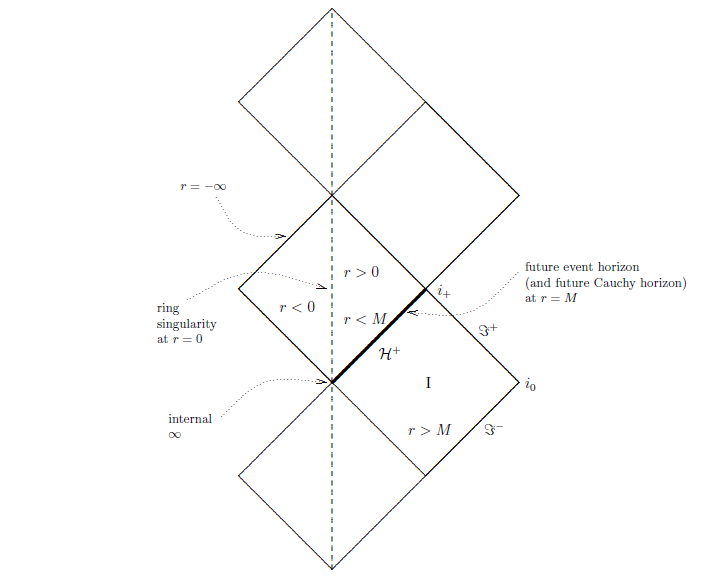
\includegraphics[scale=0.6]{immagini/kerr_causale_3.png}
    \caption{Struttura causale per Kerr estremale a $\theta =0$.}
    \label{fig.kerr_causale_3}
\end{figure}
\subsection{Ergosfera e processo di Penrose}
Calcoliamo:
\begin{equation*}
    <\partial_t, \partial_t > = g_{tt} = - \frac{\Delta - a^2\sin^2\theta}{\rho^2}= - \left(1 - \frac{2mr}{r^2+ a^2\cos^2\theta} \right)
\end{equation*}
Il vettore $\partial_t$ è di tipo tempo quando:
\begin{equation*}
    r^2 +a^2\cos^2\theta -2mr > 0
\end{equation*}
Nel caso $m^2 > a^2$ (interesse fisico) ciò avviene quando:
\begin{equation*}
    r > m + \sqrt{m^2 - a^2\cos^2\theta}
\end{equation*}
Il bordo di questa regione è un'ipersuperficie detta \textbf{ergosfera}: l'ergosfera è una superficie di tipo tempo che giace fuori dall'orizzonte $r=r_+$, ad eccezione di dove lo tocca a $\theta = 0, \pi$,  fig. \ref{fig.ergosfera}. In questi punti sull'asse di simmetria, diventa ipersuperficie nulla.
La regione interna dove $\partial_t$ può diventare di tipo spazio al di fuori dell'orizzonte degli eventi è detta \textbf{ergoregione}.


\begin{figure}
    \centering
    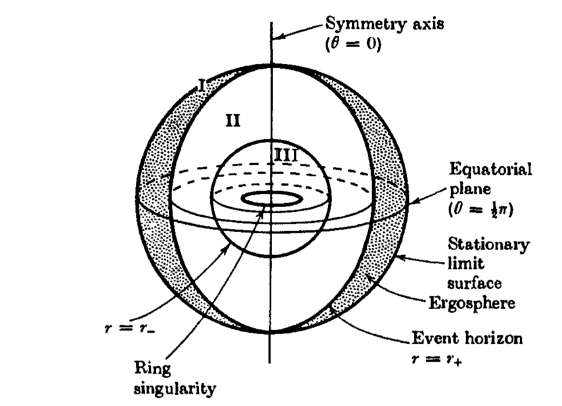
\includegraphics[scale=0.5]{immagini/ergosfera.png}
    \caption{Ergosfera del buco nero di Kerr per $m^2 > a^2$.}
    \label{fig.ergosfera}
\end{figure}

L'ergoregione permette dei processi fisici particolari: uno di questi è il \textbf{processo di Penrose}.
Consideriamo una particella che si avvicina lungo una geodetica al buco nero; chiamiamo $p$ il suo 4-momento (necessariamente tipo tempo). Per il vettore di Killing $k = \partial_t$ si identifica la costante del moto (costante lungo la geodetica):
\begin{equation*}
    E = - p\cdot k
\end{equation*}
con l'energia della particella. Se $k$ è di tipo tempo, allora $E>0$. Supponiamo che questa particella decada in due corpi, uno dei quali cade nel buco nero e uno scappa via. Per conservazione dell'energia si avrà:
\begin{equation*}
    E_2 = E - E_1
\end{equation*}
dove $E_1 = - p_1 \cdot k$ e $E_2 = - p_2 \cdot k$. Normalmente si avrà $E_1 > 0$ così che $E_2 < E$. Tuttavia se il decadimento avviene nell'ergoregione (è fuori da $r=r_+$ quindi può scappare), non vale necessariamente $E_1 > 0$, poiché $k = \partial_t$ potrebbe essere di tipo spazio. In quel caso avremmo per la particella che scappa ad infinito $E_2 > E$ ovvero l'estrazione di energia dal buco nero.

L'estrazione di energia dal buco nero ha però delle limitazioni. Per una particella che attraversa l'orizzonte $r= r_+ = m + \sqrt{m^2 - a^2}$ si ha:
\begin{equation*}
    - p_1 \cdot \xi \geq 0
\end{equation*}
dove $\xi = \partial_t + \Omega_H \partial_\phi$; quest'ultimo è un vettore nullo e future-directed sull'orizzonte (visto che è tipo tempo fuori dall'orizzonte), e $p_1$ è anch'esso future-directed e tipo tempo o nullo, a seconda che la particella sia massiva o meno. Pertanto, esplicitamente:
\begin{equation*}
    - < p_1, \partial_t > - \Omega_H < p_1, \partial_\phi > \geq 0 \iff  E_1 - \Omega_H L_1 \geq 0 
\end{equation*}
dove $L_1 = p_1 \cdot \partial_\phi$ è la componente del momento angolare della particella nella direzione di $\partial_\phi$. Otteniamo $L_1 \leq \frac{E_1}{\Omega_H}$, perciò:
\begin{equation*}
     \ E_1 < 0 \implies L_1 < 0 
\end{equation*}
Quindi in un processo di Penrose, il momento angolare del buco nero di Kerr viene ridotto. Dopo il processo, il buco nero acquisisce la massa $m + \delta m$ e momento angolare $J + \delta J$ con:
\begin{align*}
    \delta m = E_1 && \delta J = L_1
\end{align*}
e segue:
\begin{align*}
    \delta J \leq \frac{\delta m}{\Omega_H} &= \frac{\delta m}{\frac{a}{r_+^2 + a^2}} = 2m\left(m + \sqrt{m^2 - \frac{J^2}{m^2}}\right)\frac{m}{J}\delta m \\
    &= \frac{2m( m^2 + \sqrt{m^4 - J^2})}{J}\delta m
\end{align*}
ricordando che $J = ma$. Facendo qualche calcolo algebrico si può verificare facilmente che questa diseguaglianza è equivalente a:
\begin{equation*}
    \delta \left( m^2 + \sqrt{m^4 - J^2} \right) \geq 0
\end{equation*}
In un processo di Penrose la quantità tra parentesi deve aumentare. Questa ha un'interpretazione fisica che è strettamente legata ai principi termodinamici dei buchi neri, trattati con maggiore generalità in \S\ref{para.termo_bh}.

Calcoliamo l'area dell'orizzonte degli eventi del buco nero di Kerr. Per fare questo poniamoci sull'orizzonte, con $r= r_+$ ($\Delta = 0$) e $v = \textrm{cost.}$ nella metrica eq. \ref{eq.metrica_kerr_coord_kerr}, così quella indotta è:
\begin{equation*}
    ds^2 = \frac{(r^2_+ + a^2)^2}{r^2_+ + a^2\cos^2\theta}\sin^2\theta d\chi^2 + (r^2_+ + a^2\cos^2\theta)d\theta^2
\end{equation*}
da cui si ottiene la radice del determinante:
\begin{equation*}
    \sqrt{\sigma} = \left[ \frac{(r^2_+ + a^2)^2}{r^2_+ + a^2\cos^2\theta}\sin^2\theta(r^2_+ + a^2\cos^2\theta)  \right]^{1/2} = (r^2_+ + a^2)\sin\theta
\end{equation*}
Poiché siamo a raggio fissato, $d\chi = d\phi$ e pertanto ha gli stessi estremi di integrazione. L'area dell'orizzonte è quindi:
\begin{equation}
    A = \int \sqrt{\sigma}d\chi d\theta = \int_0^{2\pi}d\chi \int_0^\pi (r^2_+ + a^2)\sin\theta d\theta = 4\pi (r_+^2 + a^2)
    \label{eq.area_orizz_kerr}
\end{equation}
sostituendo $r^2_+ + a^2 = 2m(m+\sqrt{m^2 - a^2})$ e $J=ma$:
\begin{equation*}
    A = 8\pi\left( m^2 +\sqrt{m^4 - J^2}\right)
\end{equation*}
Quindi la condizione trovata prima corrisponde al secondo principio della termodinamica dei buchi neri:
\begin{equation*}
    \delta A \geq 0
\end{equation*}
E tale condizione limita la perdita di momento angolare ed estrazione di energia dal buco nero. L'area svolge il ruolo di entropia in un buco nero.

Definiamo la \textbf{massa irriducibile} del buco nero come:
\begin{equation*}
    m^2_{irr} = \frac{1}{2}\left( m^2 +\sqrt{m^4 - J^2}\right)
\end{equation*}
perciò la massa del buco nero dovrà essere tale che:
\begin{equation*}
    m^2 = m_{irr}^2 + \frac{J^2}{4m_{irr}^2} \geq m_{irr}^2
\end{equation*}
Se partiamo con un buco nero di massa $m_0$ e momento angolare $J_0$, si avrà la massa irriducibile iniziale $m_{0, irr} := m_{irr}(m_0,J_0)$. Dopo il processo di Penrose si avrà un momento angolare minore e quindi, per la relazione qui sopra:
\begin{equation*}
    m^2 \geq m^{2}_{irr} \geq m^2_{0, irr}
\end{equation*}
La condizione dell'area ci impone $\delta m^2_{irr} \geq 0$. Le quantità sono positive perciò facendone la radice otteniamo $-m \leq - m_{irr} \leq - m_{0,irr}$ ed infine:
\begin{equation*}
    m_0 - m \leq m_0 - m_{irr} \leq m_0 - m_{0, irr}
\end{equation*}
Il primo termine $m_0 - m$ equivale all'energia estratta dal processo che dovrà pertanto essere minore di $m_0 - m_{0, irr}$. Quest'ultima può essere interpretata come l'energia associata alla rotazione del buco nero, prima del processo. L'energia massima estraibile, corrispondente a $\delta m^2_{irr} = 0$, è proprio $m_0 - m_{0,irr}$ e successivamente a ciò il buco nero avrà la temperatura $T =0$.

\subsection{Forma canonica (ADM) della metrica di Kerr e temperatura di Hawking} 
La metrica di Kerr in 4-dim può essere scritta nella forma:
\begin{equation}
    ds^2 = - N^2 dt^2 + \sigma( d\phi - \omega dt)^2 + \frac{\rho^2}{\Delta}dr^2 + \rho^2 d\theta^2
    \label{eq.metrica_kerr_adm}
\end{equation}
dove sono stati definiti:
\begin{align*}
    N^2 &= \frac{\rho^2 \Delta}{\Sigma^2} \ \ \textrm{ (lapse function)} \\
    \Sigma^2 &= (r^2 +a^2)^2 - \Delta a^2 \sin^2\theta \\
    \sigma &= \frac{\Sigma^2}{\rho^2}\sin^2\theta \\
    \omega &= \frac{2mar}{\Sigma^2} \\
    \Delta &= r^2 -2mr + a^2
\end{align*}
Questa è la metrica di Kerr nella \textbf{forma canonica di ADM (Arnowitt, Deser, Misner)}.
La lapse function ha questo nome poiché, posta davanti a $dt^2$, fornisce informazioni su come scorre il tempo. In una generica dimensione, la forma canonica di ADM è del tipo:
\begin{equation*}
    ds^2 = -N^2dt^2 + n_{ij}(dx^i - N^idt)(dx^j - N^jdt)
\end{equation*}
Il formalismo di ADM è utilizzato per formulazioni hamiltoniane della relatività generale, in particolare nella quantizzazione canonica della gravità e in approcci numerici.

Come applicazione di questa metrica, possiamo vedere come calcolare più semplicemente la temperatura di Hawking, senza passare dal calcolo della gravità superficiale.
Eseguiamo una rotazione di Wick $t \rightarrow -i\tau$ per ottenere la metrica quasi euclidea:
\begin{equation*}
    ds_E^2 = N^2 d\tau^2 + \sigma(d\phi +i \omega d\tau)^2 + \frac{\rho^2}{\Delta}dr^2 + \rho^2 d\theta^2 
\end{equation*}
Sviluppiamo vicino all'orizzonte:
\begin{equation*}
    \Delta = \Delta(r_+) + \Delta'(r_+)(r-r_+) + \dots = 2(r_+ -m)(r-r_+) + \dots
\end{equation*}
\begin{equation*}
    N^2 = N^2(r_+) + \frac{\partial N^2}{\partial r}\Big|_{r_+}(r-r_+) + \dots =\frac{r_+^2 + a^2\cos^2\theta}{(r_+^2 + a^2)^2}2(r_+ - m)(r- r_+) + \dots
\end{equation*}
La metrica diventa:
\begin{align*}
    ds^2 \xrightarrow{r \rightarrow r_+} &\frac{r_+^2 + a^2\cos^2\theta}{(r_+^2 + a^2)^2}2(r_+ - m)(r- r_+) d\tau^2 + \frac{r_+^2 + a^2\cos^2\theta}{2(r_+ - m)(r- r_+)}dr^2 + \\
    & + \sigma_+(d\phi + i\omega_+ d\tau)^2 + \rho_+^2 d\theta^2
\end{align*}
Ponendo $R^2 = r- r_+$ otteniamo:
\begin{equation*}
    ds^2 \xrightarrow{r \rightarrow r_+} \frac{2(r_+^2 + a^2\cos^2\theta)}{r_+ - m}\left[ \frac{(r_+ -m)^2}{(r_+^2+ a^2)^2}R^2d\tau^2 + dR^2\right]
\end{equation*}
In questo modo la metrica è conforme a Minkowski se facciamo la corretta identificazione per $\tau$: otteniamo una singolarità conica a meno che:
\begin{equation*}
    \tau \sim \tau + 2\pi\frac{r_+^2 + a^2}{r_+ - m} \qquad \kappa = \frac{r_+-m}{r_+^2+a^2}
\end{equation*}
Così si ottiene la temperatura di Hawking per il buco nero di Kerr:
\begin{equation}
    T_H = \frac{r_+ - m}{2\pi(r_+^2 + a^2)} = \frac{r_+ - m}{4\pi m r_+}
    \label{eq.temp_hawking_kerr}
\end{equation}
Nel caso estremale $r_+ = m$ la temperatura è nulla.
\subsection{Trascinamento dei sistemi di riferimento inerziali}
Un altro fenomeno associato all'ergoregione è il cosiddetto \textit{frame dragging} o trascinamento del sistema di riferimento: i corpi nell'ergoregione non possono stare a coordinata $\phi = \textrm{cost.}$, ma sono costretti a ruotare nella stessa direzione del buco nero, altrimenti dovrebbero muoversi a velocità superluminari.
Questo effetto, come vedremo fra poco, è legato nuovamente alla natura della componente $g_{tt}$ che in questa regione cambia di segno e diventa tipo spazio (dunque i corpi non possono seguire in maniera causale una traiettoria statica con $r, \theta, \phi = \cost$).

Consideriamo quindi una linea di mondo di tipo tempo con $u$ il suo vettore tangente: $u^2 < 0$.
Esplicitamente, usando la forma di ADM, eq. \ref{eq.metrica_kerr_adm}:
\begin{equation*}
    g_{tt}u^tu^t + g_{\phi\phi}u^\phi u^\phi + g_{\theta\theta}u^\theta u^\theta + g_{rr}u^r u^r + 2g_{t\phi}u^t u^\phi < 0
\end{equation*}
Si ha che i termini in $g_{\phi\phi}, g_{\theta\theta}, g_{rr}$ sono positivi (tipo spazio) e anche $g_{tt} > 0$ poiché nell'ergoregione. Perciò si deve avere $g_{t\phi}u^t u^\phi < 0$ e poiché $g_{t\phi} = - \omega \sigma < 0$ dalla definizione della metrica eq. \ref{eq.metrica_kerr_adm}, allora il segno di $u^t u^\phi$ dovrà essere positivo. 

Mostriamo che $u^t > 0$.  Consideriamo $\xi = \partial_t + \omega \partial_\phi$, $< \xi, \xi > = -N^2 < 0$; $\xi$ è di tipo tempo al di fuori dell'orizzonte, mentre è nullo sull'orizzonte di cui è generatore. Inoltre è future-directed in quanto all'infinito $\omega \sim r^{-3} \rightarrow 0$ e rimane $\partial_t $ che è future-directed.
Poiché anche $u$ è timelike, future-directed, si ha che $< u, \xi > < 0$. Nel dettaglio:
\begin{equation*}
    <u, \partial_t > + \omega < u, \partial_\phi > \ < 0
\end{equation*}
\begin{equation*}
    < u^t \partial_t + u^\phi \partial_\phi + u^\theta \partial_\theta + u^r\partial_r, \partial_t > + \omega < u^t \partial_t + u^\phi \partial_\phi + u^\theta \partial_\theta + u^r\partial_r, \partial_\phi > \ < 0 \\
\end{equation*}
Poiché non vi sono termini in $g_{\theta t}, g_{rt}, g_{\theta\phi}, g_{r\phi}$ rimangono:
\begin{equation*}
    u^t g_{tt} + u^\phi g_{\phi t} + \omega( u^t g_{\phi t} + u^\phi g_{\phi\phi}) <0
\end{equation*}
\begin{equation*}
    u^t( -N^2 + \omega^2\sigma) +u^\phi(-\omega \sigma) +\omega( u^t(-\omega\sigma) + u^\phi\sigma) <  0
\end{equation*}
Semplificando rimane $-N^2 u^t < 0$ e quindi $u^t > 0$.

Dunque si ha che $u^\phi > 0$ ovvero, rispetto un parametro affine $\tau$:
\begin{equation*}
    u^\phi = \frac{d\phi}{d\tau} > 0
\end{equation*}
Quindi come detto la coordinata di rotazione intorno all'asse non può rimanere costante in questa regione e il corpo è costretto a rimanere in rotazione col buco nero. Può tuttavia ancora fuggire da esso, poiché è fuori dall'orizzonte degli eventi.

\subsection{Generalizzazioni di Myers-Perry}
Vediamo ora delle generalizzazioni alla soluzione di Kerr per dimensioni maggiori. In generale per $R_{\mu\nu} =0 $ e $d \geq 4$ il gruppo di isometrie è $SO(d-1)$ dal quale ci sono $\lfloor\frac{d-1}{2}\rfloor$ Casimir distinti; questi sono i parametri indipendenti di un generale tensore momento angolare. Un buco nero rotante generico avrà quindi $n+1$ parametri caratterizzanti: la massa $m$ e gli $n$ momenti angolari commutanti.
Il motivo per cui soluzioni a dimensione maggiore sono interessanti sono proprio queste nuove direzioni di rotazione possibili: buchi neri in più dimensioni assumono forme particolari e infatti si parla di \textit{black ring}, \textit{black saturn} \dots. Una review di questo tipo di soluzioni è stata fatta da R. Myers stesso in \cite{myers}.

Consideriamo quindi in $d \geq 4$, per semplicità, la soluzione \virgolette{single spinning} nella quale una sola componente rotante è presente. La metrica è:
\begin{align}
    ds^2 &= -dt^2 + \frac{\mu}{r^{d-5}\rho^2}(dt + a\sin^2\theta d\phi)^2 + \frac{\rho^2}{\Delta}dr^2 + \rho^2d\theta^2 + \nonumber \\
    &(r^2 + a^2)\sin^2\theta d\phi^2 +r^2\cos^2\theta d\Omega^2_{d-4}
    \label{eq.metrica_myers_perry_singlespinning}
\end{align}
con $\rho^2 = r^2 +a^2\cos^2\theta$, $\Delta = r^2 + a^2 - \frac{\mu}{r^{d-5}}$ e $\mu$ un parametro di massa. Questa soluzione ha orizzonte nella soluzione più grande di $\Delta = 0$:
\begin{itemize}
    \item $d=5$ l'orizzonte esiste solo per $\mu > a^2$
    \item $d > 5$ c'è sempre orizzonte, senza limiti sul momento angolare
\end{itemize}

Anche in questo caso, come nell'estremale i Reissner-Nordstr\"om, si può investigare la \virgolette{competizione} tra l'attrazione gravitazionale e la repulsione centrifuga considerando:
\begin{equation*}
    \frac{\Delta}{r^2} -1 = - \frac{\mu}{r^{d-3}}+ \frac{a^2}{r^2}
\end{equation*}
Il primo termine a destra corrisponde al potenziale gravitazionale newtoniano generalizzato, mentre il secondo termine è quello centrifugo, con dipendenza $r^{-2}$. Viene mantenuta questa dipendenza poiché, nonostante siamo in maggiori dimensioni, la rotazione avviene sempre in un piano e quindi il termine centrifugo rimane invariato. Si deduce che per:
\begin{itemize}
    \item $d=4$ vince il potenziale gravitazionale e c'è limite a Kerr ovvero non si può avere un momento angolare grande arbitrariamente (come già osservato nel caso non causale $m^2 < a^2$).
    \item $d >5$ vince il potenziale centrifugo e non c'è limite alla rotazione.
\end{itemize}
Come conseguenza della rotazione non limitata del caso a $d>5$, c'è la possibilità di assumere valori $a$ molto grandi e in questo caso si parla di \textit{ultra spinning Myers-Perry}: per valori sufficientemente elevati di $a$ si ha la situazione di uno \textit{spinning pancake}.

\subsection{Near Horizon limit del Kerr estremo}
Torniamo al Kerr in 4-dim per considerare nuovamente il caso estremo. Con Reissner-Nordstr\"om si era visto che la geometria vicino all'orizzonte era del tipo $AdS_2 \times S^2$. Vediamo cosa succede nel Kerr con $m=a$, $r_+ =r_-= m$ oltre a determinare $T_H = 0$ e $\omega_H = \frac{1}{2m}$. La metrica in coordinate di Boyer-Lindquist è:
\begin{equation*}
    ds^2 = - \frac{\Delta}{\rho^2}\left(d\hat{t}^2 -a^2 \sin^2\theta d\hat{\phi}\right)^2 + \frac{\sin^2\theta}{\rho^2}\left((\hat{r}^2 + a^2)d\hat{\phi} - ad\hat{t} \right)^2 + \rho^2 d\theta^2 + \frac{\rho^2}{\Delta}d\hat{r}^2
\end{equation*}
dove $\Delta = (\hat{r} - a)^2$. Per ottenere il limite vicino all'orizzonte si introduce un parametro di scaling $\lambda\rightarrow 0$ nelle nuove coordinate:
\begin{align*}
    r &= \frac{\hat{r}-m}{\lambda m} \\
    t &= \frac{\lambda \hat{t}}{2m} \\
    \phi &= \hat{\phi} - \frac{\hat{t}}{2m}
\end{align*}
che vengono mantenute fisse mentre si manda $\lambda$ a zero. In questo limite la metrica diventa:
\begin{equation*}
    ds^2 = 2\Omega^2 J\left[ \frac{dr^2}{r^2}  - r^2dt^2 + d\theta^2 + \Lambda^2(d\phi +rdt)^2\right]
\end{equation*}
con $\Omega^2 = \frac{1}{2}(1+\cos^2\theta)$ e $\Lambda =\frac{2\sin\theta}{1+\cos^2\theta}$.
Si può riconoscere dai  primi due termini $AdS_2$, tuttavia Kerr non risulta spazio prodotto poiché $\Omega^2(\theta)$. Se consideriamo però $\theta = \textrm{cost.} =: \theta_0$ e fissato tale che $\Lambda(\theta_0) = 1$, allora si ottiene $AdS_3$.
Il gruppo di isometrie è $SL(2, \mathbb R) \times U(1)$; il primo segue come gruppo di isometrie di $AdS_2$, mentre il secondo dalle traslazioni di $\phi$. In questa maniera il near horizon di Kerr è molto simile a quello di Reissner-Nordstr\"om.
\chapter{Struttura causale}
Ad ogni punto $p$ dello spaziotempo, si associa un cono di luce, formato dalle geodetiche nulle emesse o assorbite dall'evento; nel cono si distinguono due regioni che nominiamo \emph{futuro} e \emph{passato}. Tutti gli eventi che giacciono all'interno del cono del futuro, rappresentano tutti quegli eventi che possono essere raggiunti da una particella massiva che parta da $p$, pertanto si dice che questi eventi costituiscano il futuro cronologico di $p$. Tutti gli eventi del futuro cronologico di $p$ e compresi quelli del cono del futuro, rappresentano gli eventi che possono essere in principio influenzati da $p$ e pertanto si parla di futuro causale di $p$.

In relatività generale la struttura causale dello spaziotempo è localmente della stessa natura dello spaziotempo piatto della relatività ristretta. Quando però si vengono a trattare topologie non banali, spazitempo singolari o quant'altro, emergono le differenze rispetto il caso noto.

Scopo di questa sezione è introdurre la descrizione della struttura globale dello spaziotempo facendo uso delle trasformazioni conformi e rappresentandola per mezzo dei \textbf{diagrammi di Penrose}. Come obiettivo finale c'è la descrizione rigorosa del concetto di buco nero.

I diagrammi di Penrose permettono di rappresentare questa struttura dopo che sia stata \textbf{compattificata} la topologia. Le varietà che sono state trattate sono varietà non compatte\footnote{Una varietà topologica si dice compatta se ogni suo ricoprimento aperto contiene un sottoricoprimento finito. Gli spazi illimitati (i.e. con diametro infinito o senza bordi) non possono essere compatti.}, compattificarle consiste nel portare l'infinito ad una distanza finita. Tale processo verrà effettuato volendo mantenere a 45 gradi i coni di luce.

\section{Definizioni formali della causalità}
\begin{definizione}
 Sia uno spaziotempo $(\mathcal{M},g)$ e un punto $x$ in esso. Il cono di luce $C_x$ è definito da quei vettori $v \in T_x\mathcal{M}$ tali che $-(v^0)^2 + \sum (v^i)^2 = 0$. Se è possibile definire un semicono futuro $C^+_x$ dato dai vettori $v_\mu v^\mu =0$, $v^0 \geq 0$ (\textit{future directed}) e un semicono passato $C^-_x$ dato dai vettori $v_\mu v^\mu = 0$, $v^0 \leq 0$ (\textit{past directed}), allora $T_x\mathcal{M}$ è \textbf{orientabile nel tempo.}

Se è possibile orientare nel tempo $T_x$  $\forall x \in \mathcal{M}$ in maniera continua, allora si dice che lo spaziotempo $\mathcal{M}$ è orientabile nel tempo.
\end{definizione}

Per quanto naturale come definizione, non è detto che tutti gli spazitempo possano essere orientabili nel tempo;  un esempio è lo spaziotempo ottenuto dai  punti $p, p'$  nel de Sitter mostrato in fig. \ref{fig.spazio_desitter}: questo spaziotempo è ottenuto dai punti identificati tramite riflessioni rispetto l'origine dello spazio di immersione. In questo spazio ci sono delle curve chiuse, non omotope a zero e per le quali l'orientamento del tempo è inverso. 

Quando uno spaziotempo $(\mathcal{M}, g)$ non è orientabile nel tempo, esiste uno spazio di doppio ricoprimento $(\tilde{\mathcal{M}},g)$ che lo è \cite{hawking}.

Consideriamo quindi spazitempo orientabili nel tempo. Possiamo far uso della divisione in future/past directed per definire:
\begin{definizione}
    Sia un punto $p \in \mathcal{M}$. Chiamiamo $I^+(p)$ \textbf{futuro cronologico} di $p$, l'insieme dei punti dello spaziotempo raggiungibili da $p$ con una curva di tipo tempo future directed.
    \begin{equation*}
        I^+(p)=\left\{ q \in \mathcal{M} | \exists C:[a,b]\rightarrow \mathcal{M}, C(a)= p, C(b)= q, \Dot{C}_\mu \Dot{C}^\mu < 0, \Dot{C}^0 >0 \right\}
    \end{equation*}
Definizione analoga per $I^-(p)$ \textbf{passato cronologico} di $p$, dove si richiede però che sia past directed.

Si definisce $J^+(p)$ \textbf{futuro causale} di $p$, l'insieme dei punti raggiungibili da $p$ con una curva non-tipo spazio ($\Dot{C}_\mu \Dot{C}^\mu \leq 0$) future directed. Analogo per $J^-(p)$ il \textbf{passato causale} di $p$.
\end{definizione}
Marginalmente, $I^+(\mathcal{S})$ rispetto un insieme $\mathcal{S}$, è un aperto poichè se un qualsiasi punto $q \in \mathcal{M}$ può essere raggiunto da una curva tipo tempo future directed da $\mathcal S$, allora esiste un intorno di $q$ che può essere raggiunto in tale modo.

\begin{definizione}
Definiamo:
\begin{itemize}
    \item $i_0$ l'infinito spaziale
    \item $i_\pm$, rispettivamente, l'infinito temporale futuro e passato
    \item $\mathcal{I}^\pm$, rispettivamente, l'infinito nullo futuro e passato
    \item $\mathcal{I} = \mathcal{I}^+ \cup \mathcal{I}^-$ l'infinito nullo
\end{itemize}
\end{definizione}

\begin{definizione}
Sia $p \in \mathcal{M}$. Si dice in $p$ vale la \textbf{causalità forte} se ogni intorno di $p$ contiene un intorno di $p$ che non viene intersecato più di una volta da ogni curva causale (non-\textit{spacelike}).
Lo spaziotempo è detto fortemente causale se la condizione vale $\forall p \in \mathcal{M}$.
\end{definizione}
Dunque se in un punto $p$ vale la causalità forte, non possono esistere curve causali che ritornano arbitrariamente vicino a $p$: in particolar modo non ci possono essere curve chiuse di tipo tempo o luce. Questa condizione permette di definire la \virgolette{forma} che possono avere le curve nello spaziotempo.

Sempre legata alla discussione della struttura causale dello spaziotempo, vi è il problema dei dati iniziali e di quali punti dello spaziotempo ne determino altri. Nella teoria newtoniana, dove le azioni a distanza sono istantanee, per predire eventi in punti futuri dello spaziotempo serve \virgolette{solamente} conoscere le condizioni dell'universo al tempo presente più alcune condizioni al bordo (come i potenziali che vanno a zero a infinito). Nella teoria relativistica, poiché differenti punti possono essere legati causalmente solo se possono essere connessi da curve non tipo spazio, la conoscenza dei dati di un determinato insieme $\mathcal{S}$ dello spaziotempo potrà determinare i soli eventi in una regione detta $D^+(\mathcal{S})$. Nel dettaglio:
\begin{definizione}
Definiamo $\Sigma$ una \textbf{superficie di Cauchy parziale} un'ipersuperficie di tipo spazio dello spaziotempo che non viene intersecata da alcuna curva causale più di una volta.
\end{definizione}
Possiamo quindi definire la regione prima anticipata:
\begin{definizione}
Si definisce il \textbf{future domain of dependence} $D^+(\Sigma)$ di $\Sigma$, l'insieme dei punti $p \in \mathcal{M}$ per i quali ogni curva causale inestensibile nel passato e che contiene $p$, interseca $\Sigma$.
\end{definizione}
II significato di $D^+(\Sigma)$ (e analogamente di $D^-(\Sigma)$) è che il comportamento delle soluzioni iperboliche alle equazioni alle derivate parziali date dalle equazioni di Einstein, al di fuori di $D^+$ non può essere determinato dai dati iniziali su $\Sigma$.  Il confine futuro di questa regione, formalmente $\overline{D^+(\Sigma)}\smallsetminus I^-(D^+(\Sigma))$, è \textbf{l'orizzonte di Cauchy futuro} di $\Sigma$. 
\begin{definizione}
Una superficie parziale di Cauchy $\Sigma$ è detta essere una \textbf{superficie di Cauchy} (globale) se vale:
\begin{equation*}
    D(\Sigma) := D^+(\Sigma) \cup D^-(\Sigma) = \mathcal{M}
\end{equation*}
Uno spaziotempo $\mathcal{M}$ che ha una superficie di Cauchy è detto \textbf{globalmente iperbolico}.
\end{definizione}
Si noti bene che la proprietà di un'ipersuperficie di essere di Cauchy non è propria della superficie, ma dello spaziotempo stesso nel quale è immersa. Se $\mathcal M$ non è globalmente iperbolica, allora $D^+(\Sigma)$ o $D^-(\Sigma)$ avranno un boundary in $\mathcal{M}$ che è proprio l'orizzonte di Cauchy futuro/passato.
\begin{figure}
    \centering
    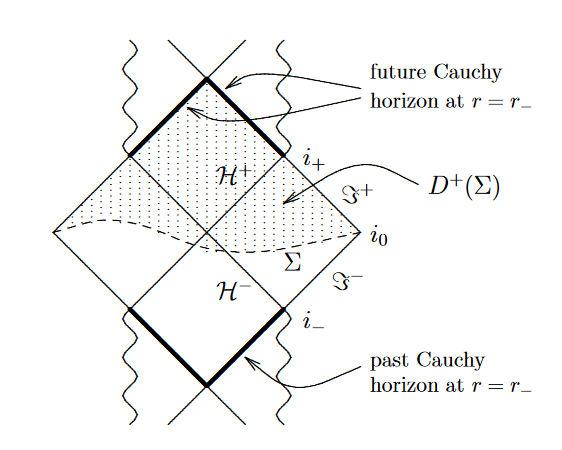
\includegraphics[scale=0.5]{immagini/cauchy_horizon.png}
    \caption{Esempio di superficie parziale di Cauchy, future domain of dependence e relativi orizzonti futuro/passato di Cauchy nella massima estensione analitica dello spaziotempo di Reissner-Nordstr\"om.}
    \label{fig.cauchy_horizon}
\end{figure}
Un esempio di superficie di Cauchy è l'ipersuperficie $t=\textrm{cost.}$ in Minkowski, mentre gli iperboloidi
\begin{equation*}
    t^2 - x^2 - y^2 - z^2 = \textrm{cost.}
\end{equation*}
sono ipersuperfici che giacciono interamente nel cono del passato dell'origine e sono solamente superfici parziali. O ancora se si considera lo spaziotempo di Minkowski privato di un punto, questo non può più ammettere superfici di Cauchy.

Con queste definizioni possiamo passare a trattare gli spazitempo utili alla descrizione dei buchi neri. Diversamente da quanto fatto per la cosmologia, dove l'interesse era quello di descrivere l'universo nella sua totalità e quindi era necessario introdurre un tensore energia-impulso che si estendesse per tutta la varietà, in questo caso ci soffermeremo su spazitempo che descrivono porzioni limitate dell'universo. L'interesse questa volta è descrivere come si comporta lo spaziotempo intorno ad una distribuzione limitata di materia, quindi per la descrizione di stelle e altri oggetti compatti. Il tensore energia-impulso sarà limitato ad una certa regione e non si estenderà all'infinito; la metrica descriverà le sole regioni esterne all'oggetto compatto. A tal fine sarà utile introdurre degli spazitempo che abbiano un comportamento semplice a distanze asintotiche.
\begin{definizione}
Uno spaziotempo orientabile nel tempo $(\mathcal{M}, g)$ è detto \textbf{asintoticamente semplice e vuoto} se esiste un embedding:
\begin{equation*}
    f: (\mathcal{M},g) \rightarrow (\Tilde{\mathcal{M}},g)\end{equation*}
che immerge $\mathcal{M}$  come varietà con bordo $\mathcal{I}$ nello spaziotempo fortemente causale $\Tilde{\mathcal{M}}$, tale che:
\begin{enumerate}
    \item Esiste una funzione differenziabile positiva $\Omega$ per cui
\begin{equation*}
    \Tilde{g}_{\mu\nu} = \Omega^2 g_{\mu\nu} \ \ \textrm{ in } \ \ \Tilde{\mathcal{M}}\cap \mathcal{M}
\end{equation*}
e vale che $\Omega = 0$ e $d\Omega \neq 0$ su $\mathcal{I}$.
\item Ogni geodetica nulla in $\mathcal{M}$ ha due estremi su $\mathcal{I}$.
\item $R_{\mu\nu}=0$ in un intorno aperto di $\mathcal{I}$ in $\Tilde{\mathcal{M}}$.
\end{enumerate}
Si scriverà $\mathcal{M}\cup \mathcal{I} = \Tilde{\mathcal{M}}$.
\end{definizione}
La prima richiesta corrisponde all'introdurre una metrica $\tilde{g}$ conforme alla metrica $g$ e più precisamente sono legate da $\Omega^2 g = f_*(\Tilde{g})$ con $f_*$ pull-back.
Le prime due richieste permettono di definire uno spaziotempo asintoticamente semplice, piuttosto generale e che include anche vari modelli cosmologici tra cui de Sitter. La terza richiesta fornisce il termine \virgolette{vuoto} e viene introdotta per restringerci ai soli spazi asintoticamente piatti.

La combinazione di $1.$ e $3.$ permette di mostrare che $\mathcal{I}$ è un'ipersuperficie nulla; il legame tra la curvatura scalare delle due metriche è ottenuto come riscalamento di Weyl \cite{wald}\cite{hawking} e ha la forma:
\begin{equation*}
    \Tilde{R} = \Omega^{-2}R - 6\Omega^{-1}\Omega_{|\mu\nu}\Tilde{g}^{\mu\nu} + 3\Omega^{-2}\Omega_{|\mu}\Omega_{|\nu}\Tilde{g}^{\mu\nu}
\end{equation*}
dove $|.$ indica la derivata covariante rispetto la metrica $\tilde{g}$. Supponendo $\Omega$ almeno di classe $\mathcal{C}^3$ su $\tilde{\mathcal{M}}$, allora $\tilde{g} \in \mathcal{C}^3$ e $\Tilde{R} \in \mathcal{C}^1$ sul bordo $\mathcal{I}$ dove $\Omega = 0$. Dunque $\Omega_{|\mu}\Omega_{|\nu}\Tilde{g}^{\mu\nu} = 0$ su $\mathcal{I}$ e poiché su questo bordo vale la condizione 1. $\Omega_{|\mu} \neq 0$, allora $\Omega_{|\nu}\Tilde{g}^{\mu\nu}$ dovrà essere un vettore nullo in quanto:
\begin{equation*}
    \Omega_{|\mu}\Tilde{g}^{\mu\nu}\Omega_{|\rho} \tilde{g}^{\rho\lambda} \Tilde{g}_{\nu\lambda} = \Omega_{|\mu}\Tilde{g}^{\mu\nu}\Omega_{|\rho}\tensor{\delta}{^\rho_\nu} = \Omega_{|\mu}\Omega_{|\rho}\Tilde{g}^{\mu\rho} = 0
\end{equation*}
dunque la ipersuperficie è nulla. Visto che $\mathcal{I}$ è una ipersuperficie nulla, si dovrà avere che $\mathcal{M}$  giaccia localmente nel passato e futuro di essa; per questo motivo $\mathcal{I}$ potrà avere soltanto due parti disconnesse $\mathcal{I}^-$ e $\mathcal{I}^+$ nelle quali si avranno gli estremi iniziali e finali delle geodetiche nulle in $\mathcal{M}$.

\'E importante notare che la richiesta $2.$ è particolarmente forte: spazi che sono asintoticamente semplici e vuoti sono, ad esempio, Minkowski e gli spazi asintoticamente piatti che descrivono oggetti legati che non vanno incontro a collasso gravitazionale; soluzioni che non rispettano la seconda condizione sono Schwarzschild, Reissner-Nordstr\"om e Kerr, per i quali esistono geodetiche nulle che non hanno \textit{endpoints} su $\mathcal{I}^+$ o $\mathcal{I}^-$. Tuttavia questi spazi hanno la caratteristica di essere asintoticamente piatti. Per questo motivo la seconda condizione viene modificata per introdurre lo spazio \textbf{debolmente asintoticamente semplice}:
\begin{enumerate}
\setcounter{enumi}{3}
\item Esiste un intorno aperto $U$ di $\mathcal{I}$ isometrico ad un intorno aperto di $\mathcal{I}'$ dello spazio asintoticamente semplice e vuoto $\mathcal{M}'$.
\end{enumerate}

\begin{teorema}
Se $\mathcal{M}$ è asintoticamente semplice e vuoto valgono:
\begin{enumerate}
    \item Ogni geodetica nulla in $\mathcal{M}$ che raggiunge $\mathcal{I}$ ha parametro affine illimitato ($\mathcal{I}^\pm$ è connessa con topologia $\mathbb{R}\times S^2$).
    \item $(\mathcal{M},g)$ è globalmente iperbolico
    \item $g$ approccia la metrica piatta di Minkowski, quindi è asintoticamente piatto.
\end{enumerate}
\end{teorema}
Le dimostrazioni possono essere trovate su \cite{hawking}. 

Per quanto riguarda il bordo $\mathcal{I}$, esso può essere pensato come all'infinito nel senso che, come detto dal teorema, qualsiasi geodetica nulla in $\mathcal{M}$ vi giunge con parametro affine illimitato. Detto $\lambda$ il parametro affine nella metrica $g$, esso è legato al parametro affine $\tilde{\lambda}$ di $\tilde{g}$ secondo:
\begin{equation*}
    \frac{d\lambda}{d\tilde{\lambda}}= \Omega^{-2}
\end{equation*}
Poiché $\Omega=0$ su $\mathcal{I}$, la quantità $\int d\lambda$ diverge e ciò spiega il primo punto del teorema. L'ultimo punto permette di dire che i diagrammi di Penrose per spazi asintoticamente semplici dovranno avere una forma condivisa con quella dello spazio di Minkowski.

\begin{definizione}
    Uno spaziotempo debolmente asintoticamente semplice e vuoto viene chiamato \textbf{asintoticamente predicibile nel futuro} se esiste una superficie di Cauchy parziale $\Sigma$ tale che:
\begin{equation*}
        \mathcal{I}^+ \subseteq \overline{D^+(\Sigma)}
\end{equation*}
dove con la barra si intende la chiusura nella varietà conforme $\tilde{\mathcal{M}}$.
\end{definizione}
Esempi di spazi che sono asintoticamente predicibili nel futuro a partire da una qualsiasi superficie $\Sigma$ sono Minkowski, Schwarzschild con $m\geq 0$, Kerr con $m\geq 0$, $m\geq |a|$ e Reissner.Nordstr\"om con $m\geq 0$, $m \geq |e|$.  La soluzione di Kerr con $m < |a|$ o Reissner-Nordstr\"om con $m < |e|$ non sono asintoticamente predicibili in quanto, per ogni superficie di Cauchy parziale $\Sigma$, ci sono curve inestensibili nel passato, di tipo tempo o nulle che partono da $\mathcal{I}^+$ e raggiungono la singolarità senza intersecare $\Sigma$. In altre parole la predicibilità asintotica del futuro può essere vista come quella condizione per la quale \textbf{non ci siano singolarità nude} nel futuro di $\Sigma$ ovvero singolarità che siano visibili da $\mathcal{I}^+$.

Possiamo infine definire il buco nero come la regione dello spaziotempo per la quale nessuna particella, massiva o massless, può fuggire verso l'infinito causale. La definizione formale è formulata \virgolette{al contrario}, andando a considerare tutti gli eventi di particelle che, nella loro evoluzione causale, hanno raggiunto l'infinito cronologico; il buco nero è quel che resta dello spaziotempo se si tolgono tutti i punti che hanno potuto raggiungere l'infinito:
\begin{definizione}
Lo spaziotempo $\mathcal{M}$ contiene un \textbf{buco nero} se
\begin{equation*}
    \mathcal{B}:= \mathcal{M}\smallsetminus J^-(\mathcal{I}^+) \neq \emptyset
\end{equation*}
La regione del buco nero viene chiamata $\mathcal{B}$, mentre il bordo di $J^-(\mathcal{I}^+)$ è detto $H$ orizzonte degli eventi.
\end{definizione}

Per chiarire ulteriormente questa definizione, in figura fig. \ref{fig.penrose_schwarz_buconero} sono evidenziate queste regioni.
\begin{figure}
    \centering
    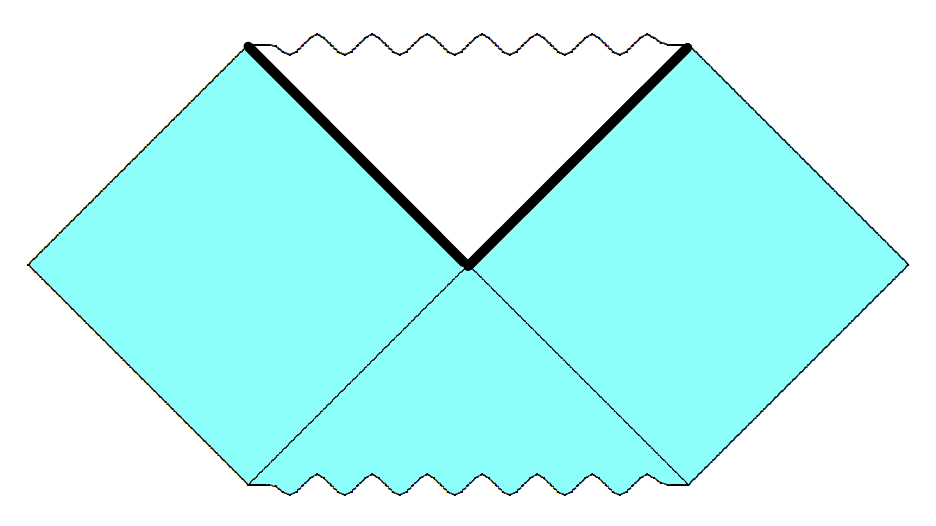
\includegraphics[scale=0.3]{immagini/schwarz_bh_regioni.png}
    \caption{In colore è mostrata la regione $J^-(\mathcal{I}^+)$, mentre quella lasciata in bianco corrisponde al buco nero. Il bordo evidenziato di nero è l'orizzonte degli eventi.}
    \label{fig.penrose_schwarz_buconero}
\end{figure}
\begin{figure}[t]
    \centering
    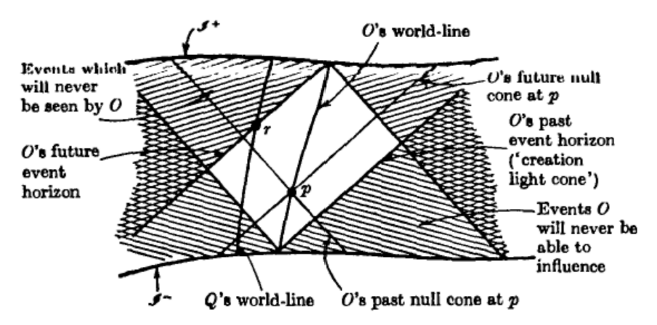
\includegraphics[scale=0.6]{immagini/horizons_hawk.png}
    \caption{Eventi che possono essere osservati o influenzati nella struttura causale di un generico spaziotempo.}
    \label{fig.orizzonti_hawk}
\end{figure}
\section{Causalità in Cosmologia}
In cosmologia risulta fondamentale introdurre nuovi tipi di orizzonti dello spaziotempo per studiare gli effetti causali tra diversi punti dell'Universo mentre questo si espande: date le dimensioni dell'Universo è importante capire quali eventi potranno essere da noi influenzati o diversamente a quali eventi noi abbiamo accesso tramite l'osservazione e quindi quale sia l'Universo osservabile. Legato a ciò vi è anche il cosiddetto \virgolette{problema dell'orizzonte} che insieme a quello della piattezza fa da apripista alla teoria dell'inflazione.

Consideriamo una famiglia di geodetiche tipo tempo, rappresentanti le linee di mondo di osservatori massivi; queste origineranno dall'infinito passato $\mathcal{I}^-$ e finiranno nell'infinito futuro $\mathcal{I}^+$. Chiamiamo $p$ un punto della geodetica di un osservatore $\mathcal{O}$: il cono nullo passato di $p$ è, come visto, il set di punti che possono essere osservati da $\mathcal{O}$ a quel tempo. Le linee di mondo di alcune particelle che intersecano questo cono nullo sono quelle viste da $\mathcal{O}$. In particolare ci sono quelle particelle le cui linee di mondo hanno origine in quei punti di $\mathcal{I}^-$ che sono intersecati dal cono passato di $\mathcal{O}$ e che delimitano un insieme di particelle che non potranno essere mai osservate da $\mathcal{O}$, fig. \ref{fig.particle_horizon_hawk}.
\begin{definizione}
La divisione di particelle che possono essere osservate da $\mathcal{O}$ in $p$ da quelle che non possono esserlo definisce l'\textbf{orizzonte delle particelle} per $\mathcal{O}$ in $p$.
\end{definizione}
\begin{figure}
    \centering
    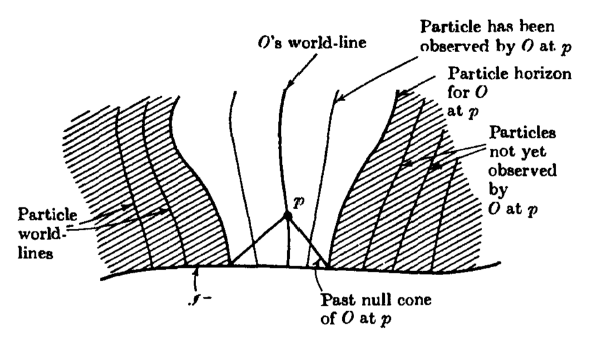
\includegraphics[scale=0.75]{immagini/particle_horizon_hawk.png}
    \caption{L'orizzonte delle particelle.}
    \label{fig.particle_horizon_hawk}
\end{figure}

L'esistenza del Big Bang impone che ci sia un tempo speciale che limita quanto indietro possiamo guardare nel passato. Indichiamo questo tempo con $t_{BB}$, ponendolo spesso a $0$. Nella cosmologia FLRW diventa:
\begin{definizione}
    L'\textbf{orizzonte delle particelle} (comovente) è la massima distanza (comovente) che ha potuto percorrere la luce dal Big Bang fino all'osservazione:
\begin{equation}
        r_{h}(t) = c\int_{t_{BB}}^t \frac{dt'}{a(t')}
        \label{eq.orizzonte_cosmologico_comovente}
\end{equation}
\end{definizione}
La distanza fisica corrispondente è data da $d_H = a(t)r_{h}(t)$ e corrisponde alle dimensioni dell'Universo osservabile. Nulla al di fuori di esso può influenzarci adesso. L'orizzonte dipende dal modello cosmologico adottato per $a(t)$ in eq. \ref{eq.friedmann_param_cosmologici}.  La definizione di orizzonte delle particelle può essere ugualmente parafrasata come \virgolette{la massima distanza con la quale ci può essere stato contatto causale dalla singolarità a una determinata epoca}.

\begin{definizione}
    L'\textbf{orizzonte degli eventi cosmologico} è la massima distanza comovente che la luce emessa ora può raggiungere un osservatore nel futuro.
    \begin{equation}
        r_{max}(t) = c \int_{t}^{t_{max}} \frac{dt'}{a(t')}
        \label{eq.event_horizon_comovente_cosmologia}
    \end{equation}
    dove $t_{max}$ è il tempo della fine dell'Universo, infinito se l'espansione non ha limite.
\end{definizione}
In altri termini, è la massima distanza che un oggetto può avere qualora venga osservato da un osservatore che osserva l'Universo al tempo $t$.
Si noti bene che l'orizzonte degli eventi cosmologico, a differenza di quello dei buchi neri, è dipendente dalla scelta dell'osservatore. 

Le proprietà degli orizzonti in cosmologia sono meglio studiate se si introduce una differente coordinata temporale.
\begin{definizione}
    Definiamo il \textbf{conformal time}:
    \begin{equation}
        \tau = \int^t_0 \frac{dt'}{a(t')} = \int_a^1 \frac{da}{a \Dot{a}} = \int_a^1\frac{da'}{a'^2 H(a')} = \int_z^0 \frac{(1+z')^2}{H(z')}dz'
        \label{eq.conformal_time}
    \end{equation}
\end{definizione}
Solitamente il conformal time è segnato con $\eta$. Di fatto è la distanza comovente divisa per la velocità della luce $c$. \'E monotona crescente e per questo motivo può essere usata come variabile temporale.
Questa coordinata permette di riscrivere la metrica FLRW, eq. \ref{eq.metrica_flrw} nella forma\footnote{Qui $\chi$ è la coordinata spaziale comovente che può essere adimensionale o dimensionata a seconda delle convenzioni, pertanto in altri luoghi potrebbe essere moltiplicata per una scala $R$ che fornisce la dimensione di lunghezza. In questo caso omettiamo la dimensione così come mettiamo $c=1$.}:
\begin{equation}
    ds^2 = a(t)^2\left[ - d\tau^2 + d\chi^2 + S_k^2(\chi)(d\theta^2 + \sin^2\theta d\phi^2)\right]
    \label{eq.metrica_flrw_conformal_time}
\end{equation}
In questo modo le curve luce sono, in un piano $(\tau, \chi)$,  delle linee a 45°. L'orizzonte delle particelle e quello cosmologico possono essere raffigurati come in fig. \ref{fig.particle_horizon_conforme}-\ref{fig.orizzonte_cosmologico_conforme}. Con questa definizione di tempo, l'orizzonte delle particelle è semplicemente:
\begin{equation*}
    r_{h} = c(\tau - \tau_{BB})
\end{equation*}
Viene altrettanto usato definire $c(aH)^{-1}$  come il \textbf{comoving Hubble radius}, mentre il raggio di Hubble proprio è solamente $cH^{-1}$. Solitamente ci si riferisce a quest'ultimo come \virgolette{l'orizzonte} in quanto fornisce una stima della distanza che la luce può percorrere mentre l'Universo si espande in una maniera apprezzabile, quindi permette di descrivere le dimensioni di regioni di Universo che sono tra loro in contatto causale. Si noti bene che rispetto l'orizzonte di particelle, il raggio di Hubble definisce la distanza di contatto causale \emph{ad una determinata} epoca, quindi risulta più utile per descrivere il contatto causale con l'evoluzione dell'Universo. Quando una determinata scala esce dall'orizzonte, si interrompe il contatto causale e si ha il \textbf{freeze out} finché non vi rientrerà.

Il comoving Hubble radius può ulteriormente essere confuso con l'orizzonte delle particelle se riscriviamo l'orizzonte delle particelle comovente di prima (ovvero il conformal time con $c=1$):
\begin{equation*}
    r_h = c \int_{t_{BB}}^t\frac{dt'}{a(t')} = \int_{\log a_{BB}}^{\log a} c(a'H)^{-1}d\log a'
\end{equation*}
Per le sorgenti di materia ordinaria, il raggio di Hubble comovente è monotono crescente col tempo e il contributo dell'integrale qui sopra è dominato nei \textit{late times}, permettendo nella cosmologia standard $r_h \sim c(aH)^{-1}$.
\begin{figure}
    \centering
    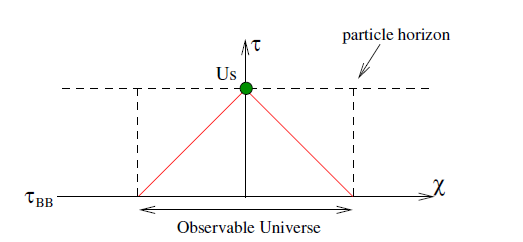
\includegraphics[scale=0.8]{immagini/particle_horizon_conforme.png}
    \caption{L'orizzonte delle particelle nel tempo conforme.}
    \label{fig.particle_horizon_conforme}
\end{figure}
\begin{figure}
    \centering
    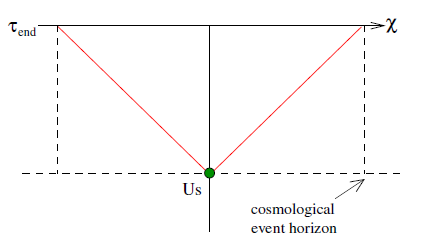
\includegraphics[scale=0.7]{immagini/orizzonte_cosmologico.png}
    \caption{L'orizzonte cosmologico nel tempo conforme}
    \label{fig.orizzonte_cosmologico_conforme}
\end{figure}
\begin{esempio}
In un Universo Einstein-de Sitter $(\Omega_0 = 1, \Omega_\Lambda =0 )$ il fattore di scala determinato dall'eq. di Friedmann, eq. \ref{eq.friedmann_param_cosmologici} evolve col tempo cosmico come $a \propto t^{2/3}$. Di conseguenza l'orizzonte di particelle comovente e proprio sono rispettivamente $r_{H,com} =3 t^{1/3} $, $r_H = 3t$, mentre il raggio di Hubble $r_{HS, com} = \frac{3}{2}t^{1/3}$, $r_{HS} = \frac{3}{2}t$ . Non esiste l'orizzonte degli eventi per questo modello. Chiamando $t_0 = \frac{2}{3}$, il tempo conforme è $\tau = 2(t/t_0)^{1/3}$ così che le precedenti comoventi diventano: $r_{H,com} = \tau$, $r_{HS, com} = \frac{\tau}{2}$.
\end{esempio}
\begin{figure}
    \centering
    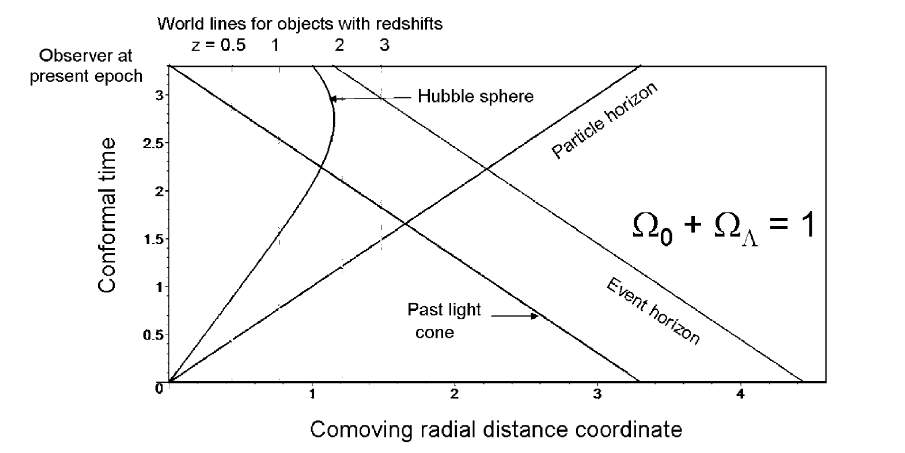
\includegraphics[scale=0.4]{immagini/lcdm_causaleconforme.png}
    \caption{Orizzonte di particelle, cono luce, orizzonte degli eventi e sfera di Hubble  in coordinate e tempo comoventi per la cosmologia standard $\Omega_0 = 0.3, \Omega_\Lambda = 0.7$. Orizzonte degli eventi e raggio di Hubble tendono a zero per $t\rightarrow \infty$: l'espansione accelerata porta le galassie a distanze dove non ci può più essere contatto causale con l'osservatore all'epoca $t$.}
    \label{fig.lcdm_causale}
\end{figure}
\section{Diagrammi di Penrose}
\subsection{Spazio Euclideo 2d}
Spieghiamo il procedimento direttamente considerando il caso semplice di $\mathbb{E}^2$.

La metrica dello spazio è:
\begin{equation*}
    ds^2 = dx^2 + dy^2 = dr^2 + r^2d\phi^2
\end{equation*}
Tale spazio risulta banale, visto che non è presente alcuna \emph{timeline}, quindi non possiede causalità. Tuttavia è istruttivo per gli esempi successivi.

L'idea per compattificare tale spazio, è quella di introdurre un cambio di coordinate del tipo $r= f(\theta)$ tale che per $r\rightarrow + \infty$ si abbia $\theta$ finito. Tra le funzioni che divergono per valori finiti, scegliamo la tangente. Questa risulterà particolarmente utile negli esempi successivi.
\begin{equation*}
    r = \tan\frac{\theta}{2} \implies dr= \frac{d\theta}{2\cos^2\frac{\theta}{2}}
\end{equation*}
così che la metrica diventa:
\begin{equation*}
    ds^2 =\frac{1}{4\cos^4\frac{\theta}{2}}[ d\theta^2 + \sin^2\theta d\phi^2]
\end{equation*}
Il prefattore diverge pertanto effettuiamo una trasformazione conforme della metrica:
\begin{equation*}
    d\tilde{s}^2 = 4\cos^4\frac{\theta}{2} ds^2 = d\theta^2 + \sin^2\theta d\phi^2
\end{equation*}
In questo modo tutti i punti di $\mathbb{E}^2$ sono stati portati sulla 2-sfera unitaria: si dice che $\mathbb{E}^2$ è conforme a $S^2$. Di fatto stiamo definendo una metrica
\begin{equation*}
    \tilde{g}_{\mu\nu}(x) = \Omega^2(x)g_{\mu\nu}
\end{equation*}
differente dall'iniziale, ma che preserva la struttura causale. 
\subsection{Spazio di Minkowski (1+1)d}
La metrica è:
\begin{equation*}
    ds^2 = -dt^2 + dx^2
\end{equation*}
con $t, x \in (-\infty,+\infty)$. Anticipiamo ora, ma lo vedremo in dettaglio nell'esempio successivo, che la compattificazione che si ottiene per lo spazio di Minkowski $(1+1)d$ è differente da quella di Minkowski $(1+3)d$ in quanto in quest'ultima, sfruttando la simmetria delle coordinate sferiche, le due variabili che dovremo trattare saranno $t, r$ dove $r \in (0,+\infty)$.

Tornando al presente caso, le strutture di interesse all'interno di Minkowski $(1+1)d$ sono rappresentate dalle rette luce $t\pm x = \textrm{cost.}$, nonché dalle rette verticali $x = \textrm{cost.}$ (rappresentanti un punto fisso spazialmente) e orizzontali $t = \textrm{cost.}$, del piano di Minkowski.

Facciamo quindi il cambio di coordinate, prendendo le outgoing e ingoing, rispettivamente:
\begin{align*}
    u = t - x && v = t + x
\end{align*}
con $u, v \in (-\infty,+\infty)$. La metrica diventa:
\begin{equation*}
    ds^2 = - dudv
\end{equation*}
Effettuiamo la compattificazione:
\begin{align*}
     u = \tan \tilde{u} && v = \tan \tilde{v}
\end{align*}
per ottenere la metrica:
\begin{equation*}
    ds^2 = - \frac{1}{\cos^2\tilde{u}\sin^2\tilde{v}}d\tilde{u}d\tilde{v}
\end{equation*}
Passando alla metrica conforme:
\begin{equation*}
    d\tilde{s}^2 = \cos^2\tilde{u}\sin^2\tilde{v} ds^2 = - d\tilde{u}d\tilde{v}
\end{equation*}

Abbiamo così compattificato lo spazio di Minkowski bidim. nelle variabili $\tilde{u}$, $\tilde{v}$, ottenendo una metrica $d\tilde{s}^2$ finita su tutto lo spazio e che preserva la struttura causale. Eseguiamo l'ultimo cambio di variabili:
\begin{align*}
\left\{\begin{array}{l}
    T = \frac{\tilde{u}+\tilde{v}}{2} \\ \\
    X = \frac{\tilde{v}-\tilde{u}}{2}
\end{array}\right.
\implies d\tilde{s}^2 =-dT^2 + dX^2
\end{align*}
dove però $T, X \in ( -\frac{\pi}{2}, \frac{\pi}{2})$. Il diagramma di Penrose, fig. \ref{fig.pen_mink_11}, è la rappresentazione grafica di tale spazio. Di fatto abbiamo potuto rappresentare tutto lo spazio di Minkowski all'interno di questo grafico. Potendo scrivere:
\begin{align*}
    t - x = \tan(T-X) && t + x = \tan(T+X) 
\end{align*}
si ottengono facilmente:
\begin{align*}
    x = \frac{1}{2}\left[ \tan(T+X) - \tan(T-X)\right] && t = \frac{1}{2}\left[ \tan(T+X) + \tan(T-X)\right]
\end{align*}
\begin{figure}
    \centering
    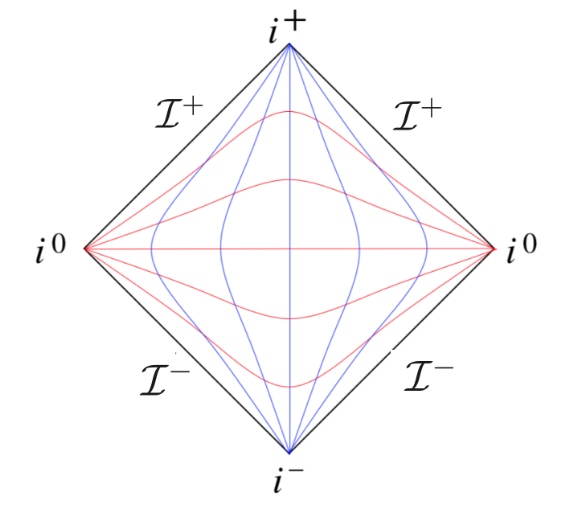
\includegraphics[scale=0.58]{immagini/penrose_mink_11.png}
    \caption{Diagramma di Penrose dello spazio Minkowski $(1+1)d$.}
    \label{fig.pen_mink_11}
\end{figure}

Nella figura sono rappresentate in blu le rette $x = \textrm{cost.}$ e in rosso $t = \textrm{cost.}$ che sono state mappate tramite la conformazione conforme nel diagramma secondo le relazioni calcolate qui sopra.

Si osserva che tutti i moti in blu nascono da un punto all'infinito $i^-$ (\emph{i minus}) detto \textbf{infinito del passato} e giungono in un tempo infinito nello stesso punto $i^+$ (\emph{i plus}) detto \textbf{infinito del futuro}. Questi sono punti di tipo tempo. La compattificazione ha proprio lo scopo di rappresentare finitamente questi infiniti che altrimenti sul piano di Minkowski non sarebbero visibili. Le curve in rosso invece originano e giungono nello stesso punto $i^0$ detto \textbf{infinito di tipo spazio}. Alcune volte si distingue in $i_L$ e $i_R$, ma sono in realtà lo stesso punto per la simmetria.

Le curve di tipo luce $t \pm x = \textrm{cost.}$ rimangono rette di 45 gradi a formare una griglia nel diagramma. Queste originano dai due lati obliqui inferiori $\mathcal{I}^-$ (\emph{scri minus}) e finisco in quelli superiori $\mathcal{I}^+$ (\emph{scri plus}). Aspetto fondamentale è che le particelle originano e finiscono tutte negli stessi punti, indipendentemente dal tipo di geodetica seguita; la luce invece ha origine per ogni punto di $\mathcal{I}^-$. In coordinate $\mathcal{I}^- = ( -\frac{\pi}{2}, \cdot)$ e $\mathcal{I}^+ =( \cdot, \frac{\pi}{2})$.

Osserviamo che si ritrova il fatto che nessuna particella massiva, che segue le curve in blu, può andare più veloce della luce in quanto qualunque sia la geodetica seguita, la tangente avrà sempre un angolo minore di 45 gradi.

Altre importanti osservazioni. Per prima cosa si ha che ogni osservatore, asintoticamente, vede tutto lo spazio nel suo passato. Questo può essere notato considerando le rette luce orientate \virgolette{verso il basso} che possono essere originate da ogni punto lungo le curve blu: stiamo parlando del cono di luce del passato. Risulta quindi evidente che quando l'osservatore si trova in $i^+$, le sue rette luce del passato coincideranno con $\mathcal{I}^+$ e quindi il suo cono del passato coinciderà con tutto lo spazio.
Per seconda cosa, qualsiasi coppia di eventi sono connessi causalmente nel passato e si possono influenzare nel futuro. Infatti se si rappresenta il cono di luce passato e futuro per ognuno dei due punti, inevitabilmente si avrà una regione di intersezione nel passato e una nel futuro. Questo aspetto è fondamentale in ambito cosmologico in quanto si ha accesso solo ad uno spazio finito e pertanto, a livello globale, il nostro universo non può essere di Minkowski.

\subsection{Spazio di Minkowski (1+3)d}
La metrica:
\begin{equation*}
    ds^2= -dt^2 + dx^2 + dy^2 + dz^2 = -dt^2 + dr^2 + r^2d\Omega_2^2
\end{equation*}
dove con $d\Omega_2$ rappresenta la 2-sfera. Applichiamo ancora il cambio di coordinate outgoing, ingoing: $u = t - r$, $v = t+ r$ per avere:
\begin{equation*}
    ds^2 =-dudv + \frac{(u-v)^2}{4}d\Omega_2^2
\end{equation*}
Compattificando con $u = \tan\tilde{u}$, $v = \tan\tilde{v}$, si ottiene:
\begin{equation*}
    ds^2 = \frac{1}{4\cos^2\tilde{u}\sin^2\tilde{v}}\left[ - d\tilde{u}d\tilde{v} + \sin^2(\tilde{v}-\tilde{u})d\Omega_2^2\right]
\end{equation*}
con $\tilde{u}, \tilde{v} \in (-\frac{\pi}{2}, \frac{\pi}{2})$. Definiamo quindi la metrica conforme:
\begin{equation*}
    d\tilde{s}^2 = - 4 d\tilde{u}d\tilde{v} + \sin^2(\tilde{v}-\tilde{u})d\Omega_2^2
\end{equation*}
Poiché $r>0$ e $r = \frac{1}{2}(v-u)$ si avrà necessariamente $v > u$ ovvero $\tilde{v} > \tilde{u}$. Ciò comporta che il diagramma non avrà la stessa forma a diamante del caso $(1+1)d$.

Definendo anche qui:
\begin{align*}
    T = \tilde{u} + \tilde{v} && R = \tilde{v} - \tilde{u}
\end{align*}
si ottiene la metrica:
\begin{equation*}
    d\tilde{s}^2 = - dT^2 + dR^2 +\sin^2R d\Omega_2^2
\end{equation*}
Si osserva che il termine $\sin^2R d\Omega_2^2$ rappresenta una 3-sfera, da pensare come una sfera con raggio che varia con lo stesso $R$. Per questioni di simmetria, nel diagramma si sopprimerà questa parte di coordinate.
Il legame con le coordinate iniziali:
\begin{align*}
    t - r= \tan\left( \frac{T - R}{2}\right) &&  t + r = \tan\left( \frac{T + R}{2}\right)
\end{align*}
con $|T| + R \leq \pi $. Il diagramma di Penrose per Minkowski $(1+3)d$ è mostrato in fig. \ref{fig.pen_mink_13}.
\begin{figure}
    \centering
    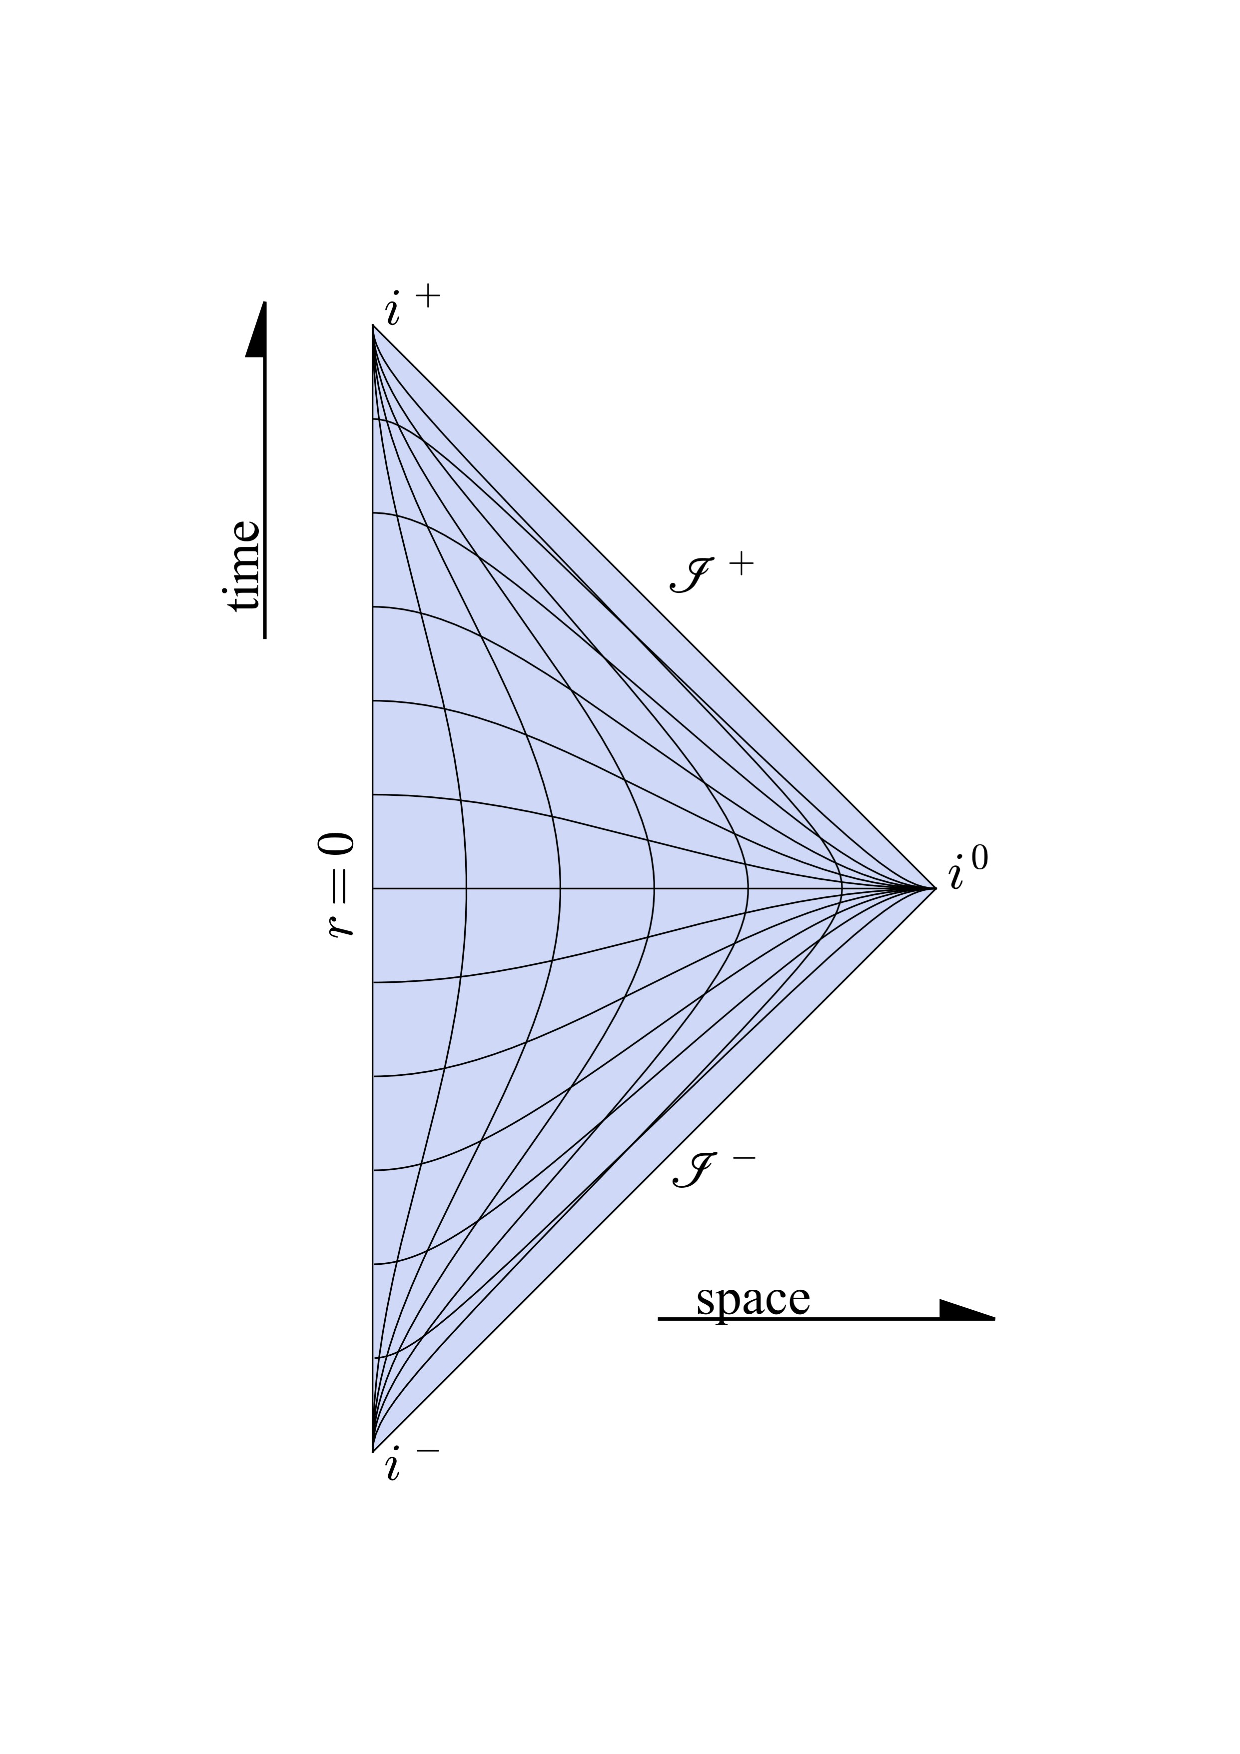
\includegraphics[scale=0.35]{immagini/mink4d.pdf}
    \caption{Il diagramma di Penrose per Minkowski $(1+3)d$.}
    \label{fig.pen_mink_13}
\end{figure}

Tale diagramma è caratterizzato da solo metà diamante per via della restrizione iniziale $r>0$ che differiva dalla richiesta iniziale $x\in\mathbb{R}$ del caso bidimensionale; tutto il bordo verticale di sinistra, corrispondente a $r=0$, non è infatti un contorno dello spazio, ma è dovuto solo a questa richiesta. Nonostante ciò sono presenti gli stessi punti di infinito $i^-$, $i^+$, $i^0$, origine e fine delle geodetiche tipo luce, spazio e $\mathcal{I}^-$, $\mathcal{I}^+$ come origine delle geodetiche nulle. Le curve relative a $t= \textrm{cost.}$ sono ottenute da:
\begin{equation*}
    t= \frac{1}{2}\left[  \tan\left( \frac{T + R}{2}\right)  -  \tan\left( \frac{T - R}{2}\right)\right]
\end{equation*}

Per lo spazio Minkowski $(1+3)d$ valgono le stesse osservazioni del caso bidimensionale, in particolare quelle esposte alla fine del precedente esempio, riguardo la possibilità di osservare tutto lo spazio in un tempo sufficientemente grande e che due qualsiasi eventi sono causalmente connessi nel passato e futuro.

\subsection{Spazio di de Sitter}
La metrica dello spazio di de Sitter statico, \S\ref{para.desitterstatici}, è:
\begin{equation*}
    ds^2 = - \left( 1 - \frac{r^2}{R^2} \right)dt^2 + \left( 1 - \frac{r^2}{R^2} \right)^{-1}dr^2 + r^2(d\theta^2 + \sin^2\theta d\phi^2)
\end{equation*}

Se effettuiamo l'embedding nello spazio di Minkowski 5-dim. di metrica:
\begin{equation*}
    ds^2 = -(dX^0)^2 + \sum_{i=1}^4 (dX^i)^2
\end{equation*}
ed effettuiamo il cambio di coordinate:
\begin{align*}
    X^0=R\sinh(\tau/R) && X^i = R\cosh(\tau/R)y^i \quad \textrm{dove} \quad \sum_{i=1}^4 (y^i)^2 = 1
\end{align*}
(questi ultimi parametrizzano la 3-sfera) si ottiene la metrica per lo spazio di de Sitter:
\begin{equation*}
    ds^2 = -d\tau^2 + R^2\cosh^2(\tau/R)d\Omega_3^2
\end{equation*}

Si definisce il \textbf{conformal time}:
\begin{equation*}
    \frac{d \eta}{d\tau} = \frac{1}{R\cosh(\tau/R)}
\end{equation*}
affinché si possa passare da $\tau \in (-\infty,+\infty)$ ad un nuovo tempo $\eta$ che sia invece finito. In particolare risolvendo si ottiene:
\begin{equation*}
    \cos \eta = \frac{1}{\cosh(\tau/R)}
\end{equation*}
così che $\eta \in (- \frac{\pi}{2}, \frac{\pi}{2})$. Facendo questo cambio di coordinate nella metrica:
\begin{equation*}
    ds^2 = \frac{R^2}{\cosh^2\eta}\left[ - d\eta^2 + d\Omega_3^2 \right] = \frac{R^2}{\cosh^2\eta}\left[ - d\eta^2 + d\chi^2 + \sin^2\chi d\Omega_2^2\right]
\end{equation*}
con $\chi \in (0,\pi)$. Risulta conformemente equivalente alla metrica:
\begin{equation*}
    d\tilde{s}^2 = - d\eta^2 + d\chi^2 + \sin^2\chi d\Omega_2^2
\end{equation*}
Omettendo la parte di simmetrica sferica, si ottiene il diagramma di Penrose di fig. \ref{fig.pen_desitter}. Tale spazio è un quadrato nel quale i punti $i^+, \mathcal{I}^+$ e $i^-, \mathcal{I}^-$ coincidono, quindi le geodetiche di tipo tempo e luce hanno stessa origine e termine. \'E importante notare che le linee verticali laterali non sono \emph{boundaries} dello spazio, ma semplicemente corrispondono ai polo nord e sud della 3-sfera. I veri limiti infiniti che sono stati compattificati sono i lati orizzontali.

A differenza dello spazio di Minkowski, non è vero che un qualsiasi osservatore, aspettando un tempo sufficiente, possa vedere tutto lo spazio. Un osservatore posto nel vertice in alto a sinistra possiede un cono del passato che riempe tutta la diagonale inferiore del quadrato e pertanto è capace di vedere solo metà dello spaziotempo; la diagonale che delimita le due regioni è l'\textbf{orizzonte degli eventi}: al di fuori di essa gli eventi non possono essere influenzati da ciò che si trova dentro.
Viceversa un osservatore posto nel vertice in basso a sinistra possiede un cono del futuro che gli permette di interagire solo con l'altra semi-regione dello spaziotempo; la diagonale delimitante viene detta \textbf{orizzonte delle particelle}: le particelle massive non possono raggiungere tutto lo spazio in un tempo finito.

Da un punto di vista cosmologico si è visto che l'attuale universo ha le caratteristiche di uno spazio di de Sitter, pertanto ci sono parti dell'universo alle quali non avremo mai accesso.
\begin{figure}
    \centering
    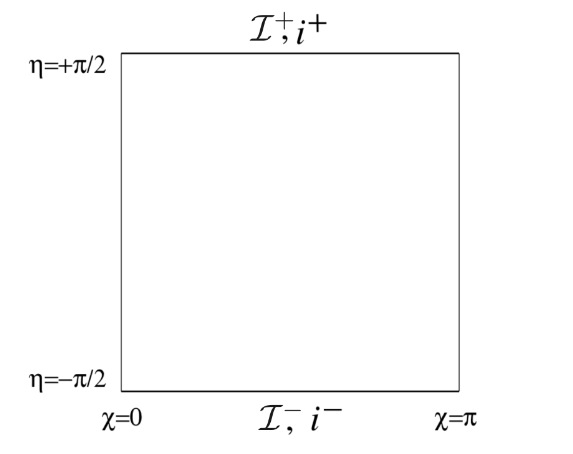
\includegraphics[scale=0.6]{immagini/desitter_penrose.png}
    \caption{Il diagramma di Penrose per lo spazio di de Sitter.}
    \label{fig.pen_desitter}
\end{figure}
\subsection{Soluzione di Schwarschild}
Il procedimento effettuato in \S\ref{para.kruskal} ha permesso di ottenere nuove importanti caratteristiche della soluzione di Schwarzschild ed in particolare, attraverso le coordinate di Kruskal-Szekeres, ci ha permesso di scrivere la metrica:
\begin{equation*}
    ds^2 = -\frac{32M^3e^{-r/2M}}{r}dUdV + r^2(U,V)d\Omega_2^2
\end{equation*}
dove si hanno giustamente i coni luce a 45 gradi, ma manca la compattificazione. Definendo come solito:
\begin{align*}
    U=\tan\tilde{U} && V = \tan\tilde{V}
\end{align*}
si ottiene:
\begin{equation*}
    ds^2 = \frac{1}{\cos^2\tilde{U}\cos^2\tilde{V}} \left[  -\frac{32M^3 e^{-r/2M}}{r}d\tilde{U}d\tilde{V} + r^2\cos^2\tilde{U}\cos^2\tilde{V}d\Omega_2^2\right]
\end{equation*}
Quindi rimuovendo il fattore conforme:
\begin{equation*}
    d\tilde{s}^2 =  -\frac{32M^3 e^{-r/2M}}{r}d\tilde{U}d\tilde{V} + r^2\cos^2\tilde{U}\cos^2\tilde{V}d\Omega_2^2
\end{equation*}

Vediamo i punti e le regioni di rilevanza per la struttura causale nelle nuove coordinate:
\begin{itemize}
    \item $r = 0$ corrisponde in coordinate di Kruskal $UV=1$ che nelle coordinate conformi:
    \begin{equation*}
        \tan\tilde{U}\tan\tilde{V} = 1 \iff \sin\tilde{U}\sin\tilde{V}-\cos\tilde{U}\cos\tilde{V}=0 \iff \cos(\tilde{U}+\tilde{V})=0
    \end{equation*}
    ovvero $\tilde{U}+\tilde{V}= \pm \frac{\pi}{2}$.
    \item $r=2M$ corrisponde a $U , V = 0$ ovvero semplicemente $\tilde{U}, \tilde{V}=0$.
    \item $r>2M$ ovvero $U, V > 0$ e cioè $\tilde{U}, \tilde{V}>0$.
\end{itemize}
Osserviamo che la scelta della tangente per compattificare, permette si semplificare molto questi calcoli. In maniera analoga si possono definire le quantità:
\begin{align*}
    T = \tilde{U}+ \tilde{V} && R = \tilde{V}- \tilde{U}
\end{align*}
da non confondere con le $T, R$ basate sulle coordinate di Kruskal. In fig. \ref{fig.penrose_schwarz} è rappresentato il diagramma della soluzione estesa di Schwarzschild (gli assi $\tilde{U},\tilde{V}$ sono ruotati in 45 gradi e corrispondono come visto sopra alle rette $r=2M$); sono anche rappresentate le quattro regioni già trattate in \S\ref{para.kruskal} corrispondenti al nostro universo (I), il buco nero (II), l'altro universo (III) e il buco bianco (IV).
\begin{figure}
    \centering
    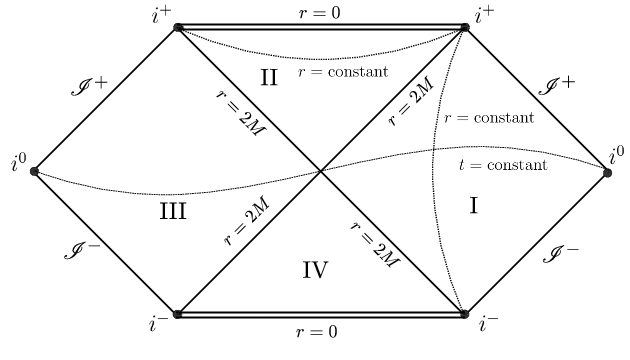
\includegraphics[scale=0.65]{immagini/penrose_schwarz.png}
    \caption{Il diagramma di Penrose della soluzione estesa di Schwarzschild.}
    \label{fig.penrose_schwarz}
\end{figure}

Limitandoci per il momento a discutere il quadrato di destra, tornano i punti di infinito $i^-$, $i^+$ per le particelle e i $\mathcal{I^-}$, $\mathcal{I}^+$ per la luce. I due bordi di sinistra corrispondono invece all'orizzonte del passato $H^-$ e l'orizzonte degli eventi $H^+$. Possiamo osservare che la metà di destra di tale quadrato condivide la stessa struttura causale dello spazio di Minkowski $(1+3)d$ e questo è dovuto al fatto che la soluzione di Schwarzschild è asintoticamente piatta. Le geodetiche che originano in $i^-$ e finiscono nell'orizzonte $H^+$ sono quelle destinate a finire nel buco nero, non potendo uscire in quanto servirebbe un'inclinazione superiore a 45 gradi.

La geodetica $t=\textrm{cost.}$ rappresentata e passante per l'origine del grafico, è il tipo di geodetica che permette di collegare i due universi (l'origine è il ponte di Einstein-Rosen già visto) che chiaramente non è percorribile in quanto implicherebbe $v>c$.

Consideriamo la geodetica di una particella che finisce nel buco nero; eventualmente consideriamo che la sua velocità sia particolarmente relativistica, linea rossa in fig. \ref{fig.penschwarz_orizz}. Immaginiamo che questo osservatore massivo emetta dei fotoni, rappresentate dalle rette luce in blu, e che questi vengano ricevuti da un altro osservatore fisso a $r = \textrm{cost.}$, in arancione.
Innanzitutto si può osservare che per tempi infinitamente lontani, si potrebbe credere che il segnale inviato dall'osservatore rosso sia invece partito dal buco bianco. L'aspetto invece fondamentale è che più l'osservatore in rosso si avvicina all'orizzonte, più sarà il tempo richiesto affinché il segnale giunga all'osservatore arancione. Al limite, quando vi si troverà all'orizzonte $H^+$, il segnale luminoso potrà giungere all'osservatore arancione solo quando esso si troverà nel suo punto di infinito $i^+$.
In altri termini, serve un tempo infinito per poter mappare tutto lo spaziotempo e poter definire l'orizzonte. Questo porta alla conclusione che \textbf{l'orizzonte degli eventi non è locale} in quanto esso è definito come il \emph{boundary} a infinito del cono del passato di una geodetica di tipo tempo (ad esempio la arancione della figura).
\begin{figure}
    \centering
    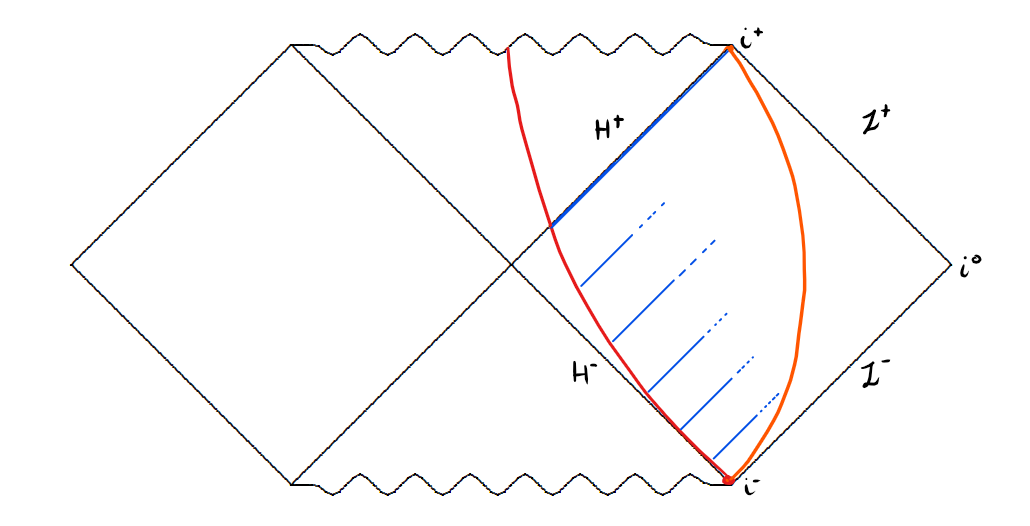
\includegraphics[scale=0.45]{immagini/penschwarz_orizz.png}
    \caption{Particella relativistica (linea rossa) che finisce nella singolarità, mentre emette fotoni (linee blu) ricevuti dall'osservatore a $r=\textrm{cost.}$ (linea arancione). Più si avvicina all'orizzonte degli eventi, più verrà richiesto un tempo al limite infinito per ricevere il segnale.}
    \label{fig.penschwarz_orizz}
\end{figure}
\subsection{Singolarità nuda in Schwarzschild}
La soluzione di Schwarzschild presenta una singolarità nuda, cioè che può essere vista a $\mathcal{I}^+$ quando $M<0$; dal punto di vista fisico ciò non ha senso, ma la soluzione soddisfa comunque le equazioni di Einstein e pertanto vale la pena analizzarla.
Partendo dalla metrica eq. \ref{eq.metricaschwarz}, la singolarità presente è solamente quella di curvatura $r=0$. Si introduce la coordinata tartaruga $ r_* = r + 2M\log\left(1-\frac{2M}{r}\right) $ e la metrica diventa:
\begin{equation*}
    ds^2 = \left(1-\frac{2M}{r}\right)(-dt^2 + dr^2_*)
\end{equation*}
Il termine $\left(1-\frac{2M}{r}\right)$ a questo punto non è più singolare. Con le coordinate nulle $u=t-r_*$, $v = t + r_*$:
\begin{equation*}
    ds^2 = - \left(1-\frac{2M}{r}\right)dudv
\end{equation*}
Possiamo ora compattificare secondo:
\begin{equation*}
    u = \tan\frac{u'}{2} \qquad v = \tan\frac{v'}{2}
\end{equation*}
così otteniamo:
\begin{equation*}
    ds^2 = - \left(1-\frac{2M}{r}\right)\frac{1}{4\cos^2\frac{u'}{2}\cos^2\frac{v'}{2}}du'dv' = \Omega^{-2}(-du'dv')
\end{equation*}
La metrica è conforme a Minkowski. In generale valgono $-\pi \leq u', v' \leq \pi$ e $r>0$ tuttavia otteniamo le condizioni:
\begin{itemize}
        \item $r=0 \iff v=u \iff v'=u'$
        \item $r>0 \iff r_*>0 \iff v>u \iff \arctan v > \arctan u \iff v'>u'$
\end{itemize}
Si ottiene che il grafico compattificato di Schwarzschild con massa negativa ha la stessa forma di Minkowski $(1+3)d$, fig. \ref{fig.pen_mink_13} con la singolarità in $r=0$ che può essere vista a $\mathcal{I}^+$.
\chapter{Integrali di Komar}
Vogliamo definire quali sono le cariche conservate per uno spaziotempo al quale sono associate delle simmetrie; ciò equivale a studiare i campi vettoriali di Killing. Una delle possibilità è tramite gli integrali di Komar.

\section{Integrali di Komar}
Sia $V \subseteq \Sigma$, dove $\Sigma$ è una ipersuperficie di tipo spazio (ad esempio $t=\cost$ in Schwarzschild) e sia $\partial V$ il bordo di $V$. Ad ogni campo vettoriale di Killing $\xi$ possiamo associare \textbf{l'integrale di Komar} $Q_\xi(V)$ definito:
\begin{equation}
    Q_\xi(V) = \frac{c}{16\pi G}\oint_{\partial V}dS_{\mu\nu}\nabla^\mu \xi^\nu
    \label{eq.integrale_komar}
\end{equation}
dove $c=\cost$, mentre $dS_{\mu\nu}$ è la misura orientata sul bordo $\partial V$. Se si usa il teorema di Gauss, eq. \ref{eq.integrale_komar} diventa:
\begin{equation}
    Q_\xi(V) = \frac{c}{8\pi G}\int_V dS_\mu \nabla_\nu\nabla^\mu \xi^\nu
    \label{eq.integrale_komar_gauss}
\end{equation}

Da eq. \ref{eq.identità_killing}, facendone la traccia si ottiene:
\begin{equation*}
    \nabla_\nu \nabla_\mu \xi^\nu = R_{\mu\nu}\xi^\nu
\end{equation*}
Così, sostituendo in eq. \ref{eq.integrale_komar_gauss} si ha;
\begin{equation*}
    Q_\xi(V) = \frac{c}{8\pi G}\int_V dS_\mu \tensor{R}{^\mu_\nu}\xi^\nu
\end{equation*}
Dalle equazioni di Einstein abbiamo che:
\begin{align*}
    R_{\mu\nu} - \frac{1}{2}Rg_{\mu\nu} = 8\pi G T_{\mu\nu} &\implies R= - 8\pi G T \\
    &\implies R_{\mu\nu} = 8\pi G(T_{\mu\nu} - \frac{1}{2}Tg_{\mu\nu})
\end{align*}
così diventa:
\begin{equation*}
    Q_\xi(V) = c\int_V dS_\mu \left( \tensor{T}{^\mu_\nu}\xi^\nu - \frac{1}{2}T\xi^\mu \right)
\end{equation*}
che possiamo riscrivere in termini di una quadricorrente $J^\mu(\xi)$ nella forma:
\begin{equation*}
    J^\mu(\xi) = c\left( \tensor{T}{^\mu_\nu}\xi^\nu - \frac{1}{2}T\xi^\mu \right)
\end{equation*}
e l'integrale di Komar è effettivamente la sua carica:
\begin{equation}
    Q_\xi (V) = \int_V dS_\mu J^\mu(\xi)
    \label{eq.integrale_komar_corrente}
\end{equation}
\begin{lemma}
La corrente $J^\mu(\xi)$ è una corrente conservata, ovvero $\nabla_\mu J^\mu(\xi) =0$.
\end{lemma}
\begin{proof}
Esplicitamente:
\begin{equation*}
    \nabla_\mu J^\mu = c\left( (\nabla_\mu \tensor{T}{^\mu_\nu})\xi^\nu + \tensor{T}{^\mu_\nu}\nabla_\mu \xi^\nu - \frac{1}{2}\xi^\mu \nabla_\mu T - \frac{T}{2}\nabla_\mu \xi^\mu \right)
\end{equation*}
Il termine $\nabla_\mu \tensor{T}{^\mu_\nu} = 0$ per la conservazione del tensore energia-impulso. Il termine $T_{\mu\nu}\nabla^\mu\xi^\nu = 0$ poiché è la contrazione di un tensore simmetrico $T_{\mu\nu}$ con una quantità che soddisfa Killing, eq. \ref{eq.killing} dunque antisimmetrica.
Per il terzo termine:
\begin{equation*}
    \xi^\mu \nabla_\mu T = \xi^\mu \partial_\mu T = - \frac{\xi^\mu}{8\pi G}\partial_\mu R
\end{equation*}
Se introduciamo delle coordinate in cui $\xi = \frac{\partial}{\partial \alpha}$ ovvero dove $\xi$ è una delle coordinate, allora la metrica non dipenderà da $\alpha$, $\frac{\partial g_{\mu\nu}}{\partial \alpha}=0$, e quindi neanche $R$. Perciò anche questo termine deve essere nullo.
Il quarto termine è a sua volta nullo poiché $\xi$ è di Killing i.e. $\nabla_\mu\xi_\nu = - \nabla_\nu\xi_\mu$, e allora $\nabla^\mu\xi_\mu = 0$.
\end{proof}

\section{Energia}
Come primo esempio particolare vediamo la carica associata al campo vettoriale di Killing delle traslazioni temporali: questa carica è l'energia.
\begin{equation}
    E(V) = - \frac{1}{8\pi G}\oint_{\partial V} dS_{\mu\nu}\nabla^\mu K^\nu 
    \label{eq.komar_energia}
\end{equation}
la costante $c = -2$ viene fissata col seguente ragionamento:
Consideriamo una metrica $g_{\mu\nu} \rightarrow \eta_{\mu\nu}$ per una certa $r\rightarrow +\infty$ in modo tale che:
 \begin{equation*}
     h_{\mu\nu} = g_{\mu\nu} - \eta_{\mu\nu} = o(\frac{1}{r})
 \end{equation*}
Allora possiamo linearizzare le equazioni di Einstein vicino $r = + \infty$ e considerare una sorgente come polvere statica ($\dot\rho = 0$) e debole così che sia descritta da:
 \begin{equation*}
     T_{\mu\nu} = diag (\rho, 0,0,0)
 \end{equation*}
In questo modo, riprendendo la definizione dell'energia ed usando le equazioni di Einstein con il teorema di Gauss:
 \begin{equation*}
     E(V) = \int_{t=\cost} dV T_{00} = \int \rho dV = -\frac{1}{8\pi G}\oint dS_{\mu\nu}\nabla^\mu K^\nu
 \end{equation*}
Leghiamola all'integrale di Komar di eq. \ref{eq.integrale_komar_corrente}; per $V =\{ t= \cost\}$ si ha che $dS_\mu = n_\mu dV$\footnote{Usiamo qui $dS^0 = dV$ e quindi $dS_0 = -dV$} con $n_\mu$ un vettore normale. Allora:
 \begin{align*}
     dS_\mu(\tensor{T}{^\mu_\nu}K^\nu - \frac{1}{2}TK^\mu) &= dS_0( \tensor{T}{^0_0}K^0 - \frac{1}{2}TK^0) = dS_0(-\rho K^0 + \frac{1}{2}\rho K^0) \\
     &= - dS_0 \rho \frac{K^0}{2} = -dV (-\rho\frac{K^0}{2})= \frac{\rho}{2}dV
 \end{align*}
 Dunque
 \begin{equation*}
     Q_K(V) = \int_V dS_\mu J^\mu = c \int \frac{\rho}{2}dV = \frac{c}{2}\int \rho dV = \frac{c}{2}E(V)
 \end{equation*}
 In questo modo si ottiene il valore della costante.

Vediamo $E(V)$ applicato alla metrica di Schwarzschild; per semplicità riscriviamo $N=\sqrt{1 - \frac{2Gm}{r}}$. Rimaniamo nella regione $r> 2m$ e consideriamo $V = \Sigma_t = \{t=\cost\}$; il suo bordo $\partial V$ è la 2-sfera corrispondente all'intersezione con $r= \cost$.
Il vettore normale a $V$ è:
\begin{equation*}
    u= N^{-1}\partial_t
\end{equation*}
ed è di tipo tempo, $<u,u> = -1$. Il vettore normale a $\partial V$ è invece:
\begin{equation*}
    v = N\partial_r
\end{equation*}
Questo è infatti di tipo spazio, $<v,v> = 1$ ed è ortogonale alla 2-sfera, $<v,\partial_\phi> = 0$, $<v, \partial_\theta > = 0$.
La misura orientata su $\partial V$ è:
\begin{equation*}
    dS^{\mu\nu} = (v^\mu u^\nu - u^\mu v^\nu)\sqrt{\sigma}d\phi d\theta
\end{equation*}
dove $\sigma$ è il determinante della metrica indotta sulla 2-sfera:
\begin{equation*}
    d\sigma^2 = r^2(d\theta^2 + \sin^2\theta d\phi^2) \implies \sqrt{\sigma} = r^2\sin\theta
\end{equation*}
Quindi la misura orientata è:
\begin{equation*}
    dS^{rt} = (v^ru^t - u^r v^t)\sqrt{\sigma} d\theta d\phi = \sqrt{\sigma}d\theta d\phi = - dS^{tr}
\end{equation*}
e l'integrale dell'energia:
\begin{equation*}
    E = - \frac{1}{8\pi G}\int_0^\pi d\theta \int_0^{2\pi}d\phi \sqrt{\sigma}\nabla_r K_t 2
\end{equation*}
Il fattore 2 arriva dal fatto che $\nabla_r K_t = - \nabla_t K_r$ e $dS^{rt} = - dS^{tr}$. Si calcola esplicitamente:
\begin{align*}
    \nabla_r K_t &= \partial_r K_t - \tensor{\Gamma}{^\rho_{rt}}K_\rho \\
    &= \partial_r K_t - \Gamma_{\rho r t}K^\rho = \partial_r K_t - \Gamma_{trt}
\end{align*}
dove:
\begin{equation*}
    \partial_r K_t = \partial_r(g_{tt}K^t) = \partial_r g_{tt}
\end{equation*}
mentre il simbolo di Christoffel, secondo eq. \ref{eq.connlevicivita}:
\begin{equation*}
    \Gamma_{trt} = \frac{1}{2}(g_{tt,r} + g_{tr,t} - g_{rt,t}) = \frac{1}{2}\partial_r g_{tt}
\end{equation*}
Dunque:
\begin{equation*}
    \nabla_r K_t = \frac{1}{2}\partial_r g_{tt}= - \frac{Gm}{r^2}
\end{equation*}

Per concludere si ricava:
\begin{equation*}
    E = - \frac{1}{4\pi G}\int_0^\pi d\theta \int_0^{2\pi}d\phi r^2\sin\theta(- \frac{Gm}{r^2}) = m 
\end{equation*}
Per Schwarzschild si ottiene che l'energia non dipende dal raggio $r$, poiché tra diversi raggi è presente il vuoto: in casi come de Sitter, dove c'è la costante cosmologica, tra diversi raggi c'è questa componente di densità di energia da considerare ad esempio.
\section{Momento angolare}
L'integrale di Komar associato al vettore di Killing $\xi = m = \partial_\phi$ è:
\begin{equation}
    J(V) = \frac{1}{16\pi G} \oint_{\partial V} dS_{\mu\nu}\nabla^\mu m^\nu
    \label{eq.komar_mom_angolare}
\end{equation}
dove la costante è fissata $c=1$. Vediamo da dove deriva. Usiamo Gauss:
\begin{align*}
    J(V) &= \frac{1}{8\pi G} \int_V dS_\mu \nabla_\nu \nabla^\mu m^\nu = \frac{1}{8\pi G}\int_V dS_\mu \tensor{R}{^\mu_\nu}m^\nu \\
    &= \int_V dS_\mu (\tensor{T}{^\mu_\nu} - \frac{T}{2}\tensor{\delta}{^\mu_\nu})m^\nu = \int_V dS_\mu J^\mu
\end{align*}
dove abbiamo definito la corrente come $J^\mu = \tensor{T}{^\mu_\nu}m^\nu - \frac{T}{2}m^\mu$. Se scegliamo l'ipersuperficie $V$ su $ \Sigma_t = \{t=\cost\}$ e $m=\partial_\phi$ allora $dS_\mu m^\mu =0$ ($g_{\mu\nu} \approx \eta_{\mu\nu}$, poiché altrimenti, usando soluzioni come Kerr, il vettore normale è $n= \partial_t + \omega \partial_\phi$ e non solo $\partial_t$). Perciò rimane solo $\tensor{T}{^\mu_\nu}m^\nu$, usando $dS_0 = dV$ e lo sviluppo in coordinate cartesiane $m= x^1\partial_2 - x^2\partial_1$:
\begin{equation*}
J = \int_V dV \tensor{T}{^0_\nu}m^\nu = \int_V dV( \tensor{T}{^0_2}x^1 - \tensor{T}{^0_1}x^2) = \epsilon_{3ik}\int_V dV x^i T^{k0}
\end{equation*}
Questo corrisponde alla terza componente del momento angolare di un campo con tensore $T_{\mu\nu}$ nello spaziotempo di Minkowski. Così è verificato che $c=1$ è corretto. Passare per il limite di campo debole è una procedura abbastanza tipica per determinare la costante $c$.

Calcoliamo $J(V)$ per la soluzione di Kerr e consideriamo la metrica nella forma di ADM, eq. \ref{eq.metrica_kerr_adm}. Il vettore normale alla ipersuperficie $\Sigma_t$ è:
\begin{equation*}
    u = N^{-1}(\partial_t + \omega \partial_\phi)
\end{equation*}
poiché verifica facilmente che $<u,u> = -1$ e $<u, \partial_i> =0$ per $i=r, \theta,\phi$. Il bordo $\partial V$ corrisponde all'intersezione con $\Sigma_t$ per $r=\cost$ ed ha come vettore normale:
\begin{equation*}
    v = \frac{\sqrt{\Delta}}{\rho}\partial_r
\end{equation*}
e infatti verifica $<v,v> = 1$, $<v, \partial_i> = 0$ con $i= \theta,\phi$.
La misura orientata su $\partial V$ è:
\begin{equation*}
    dS^{\mu\nu} = (v^\mu u^\nu - u^\mu v^\nu)\sqrt{\sigma}d\theta d\phi
\end{equation*}
dove la metrica indotta su $\partial V$ è:
\begin{equation*}
    d\sigma^2 = \rho^2d\theta^2 + \frac{\Sigma^2 \sin^2\theta}{\rho^2}d\phi^2 \implies \sqrt{\sigma} = \Sigma \sin \theta
\end{equation*}
Possiamo quindi calcolare, usando come passaggio intermedio la proprietà di Killing eq. \ref{eq.killing}:
\begin{equation*}
    (v^\mu u^\nu - u^\mu v^\nu )\nabla_\mu m_\nu = v^\mu u^\nu \nabla_\mu m_\nu - u^\mu v^\nu \nabla_\mu m_\nu = - 2u^\mu v^\nu \nabla_\mu m_\nu
\end{equation*}
Quindi l'integrale eq. \ref{eq.komar_mom_angolare}:
\begin{equation*}
    J(V) = -\frac{2}{16\pi G}\int_0^{\pi}d\theta \int_0^{2\pi}d\phi \Sigma \sin\theta u^\mu v^\nu g_{\nu\rho}\nabla_\mu m^\rho
\end{equation*}
Poiché la derivata covariante si riduce a:
\begin{equation*}
    \nabla_\mu m^\rho = \partial_\mu m^\rho + \tensor{\Gamma}{^\rho_{\mu\sigma}}m^\sigma = \tensor{\Gamma}{^\rho_{\mu\phi}}
\end{equation*}
l'integrale diventa:
\begin{align*}
    J(V) &= - \frac{1}{4 G}\int_0^\pi d\theta \Sigma \sin \theta u^\mu v^\nu \tensor{\Gamma}{^\rho_{\mu\phi}} \\
    &= - \frac{1}{4 G}\int_0^\pi d\theta \Sigma\sin\theta \left(u^tv^r \Gamma_{rt\phi} + u^\phi v^r \Gamma_{r\phi\phi} \right) \\
    &= - \frac{1}{4G} \int_0^\pi d\theta \Sigma\sin\theta\left(\frac{\sqrt{\Delta}}{N\rho}\Gamma_{rt\phi} + \frac{\omega\sqrt{\Delta}}{N\rho}\Gamma_{r\phi\phi} \right)
\end{align*}
Da eq. \ref{eq.connlevicivita} si calcolano:
\begin{align*}
    \Gamma_{rt\phi} &= - \frac{1}{2}\partial_r\left( \frac{-\omega\Sigma^2\sin^2\theta}{\rho^2}\right) \\
    \Gamma_{r\phi\phi} &= - \frac{1}{2}\partial_r\left( \frac{\Sigma^2\sin^2\theta}{\rho^2}\right)
\end{align*}
Questi termini dipendono da $r$, ma siccome ci troviamo dove $r=\cost$, si ottiene lo stesso se si sviluppa per $r\rightarrow +\infty$. Facendo le sostituzioni e calcolando le derivate parziali, si ottiene che in questo limite:
\begin{align*}
    \Gamma_{rt\phi} &\sim -\frac{ma\sin^2\theta}{r^2} \\
    \Gamma_{r\phi\phi} &\sim -r\sin^2\theta  
\end{align*}
Mentre i loro prefattori che appaiono nell'integrale:
\begin{align*}
    \frac{\sqrt{\Delta}}{N\rho} &\sim 1 \\
    \frac{\omega\sqrt{\Delta}}{N\rho} &\sim \frac{2ma}{r^3}
\end{align*}
Così, considerando che $\Sigma \sim r^2$ e che $\int_0^\pi \sin^3\theta d\theta = \frac{4}{3}$, si ottiene:
\begin{equation*}
    J = -\frac{1}{4G}\int_0^\pi d\theta \sin\theta\Sigma(-\frac{3ma\sin^2\theta}{r^2}) = \frac{3ma}{4G}\int_0^\pi d\theta \sin^3\theta = \frac{ma}{G}
\end{equation*}
Il momento angolare per il buco nero di Kerr è pertanto:
\begin{equation*}
    J = \frac{ma}{G}
\end{equation*}
In questo modo è giustificata la formula che è stata utilizzata in tutta la precedente trattazione.
\chapter{Buchi neri}
In questo capitolo verranno investigate maggiormente le proprietà dei buchi neri, in particolar modo le proprietà dell'orizzonte per poi trattare il legame con la termodinamica e la radiazione di Hawking. Si farà infine un accenno ad buco nero di Banados-Teitelboim-Zanelli.
\section{Ipersuperfici nulle e gravità superficiale}
\begin{definizione}
Sia $S(x)$ una funzione liscia sullo spaziotempo di coordinate $x^\mu$ e si considerino la famiglia di ipersuperfici $S = \textrm{cost.}$. I \textbf{campi vettoriali normali all'ipersuperficie} sono definiti da:
\begin{equation}
    l = \Tilde{f}(x)(g^{\mu\nu}\partial_\nu S) \frac{\partial}{\partial x^\mu}
    \label{eq.vettore_normale_ipersup}
\end{equation}
per una qualche funzione non nulla $\Tilde{f}$. Se $l^2 = 0$ per una qualche ipersuperficie $N$ nella famiglia, allora $N$ è una \textbf{ipersuperficie nulla}.
\end{definizione}
Tra le varie ipersuperfici nulle di nostro interesse, c'è l'orizzonte degli eventi. Vediamo quindi le loro proprietà.

Sia $N$ un'ipersuperficie nulla con $l$ vettore normale e sia $\phi$ un vettore tangente a $N$, ovvero $<\phi, l> = 0$.  Siccome $l$ è un vettore nullo, $<l,l> = 0$ allora $l$ è anche un vettore tangente. Pertanto in un'ipersuperficie nulla i \textbf{vettori normali sono anche tangenti}. Essendo un vettore tangente, esisterà la sua curva integrale (nulla) $x^\mu$ in $N$ tale che $l^\mu = \frac{dx^\mu}{d\lambda}$, rispetto $\lambda$ parametro della curva.
Per queste curve nulle sull'ipersuperficie nulla si ha il lemma:
\begin{lemma}
Le curve $x^\mu$ sono geodetiche.
\end{lemma}
\begin{proof}
Sia $N$ il membro $S=0$ della famiglia (non necessariamente nulla) di ipersuperfici $S(x^\mu) = \textrm{cost.}$
Consideriamo la scrittura di $l^\mu$ di eq.\ref{eq.vettore_normale_ipersup}. Per verificare sia una geodetica, calcoliamo la derivata covariante lungo $l$ del vettore stesso:
\begin{align}
    \nabla_l l^\mu &= l^\rho \nabla_\rho l^\mu =  l^\rho \nabla_\rho (\Tilde{f}(x)g^{\mu\nu}\partial_\nu S ) = (l^\rho \partial_\rho \Tilde{f}) g^{\mu\nu}\partial_\nu S + \Tilde{f}g^{\mu\nu}l^\rho \nabla_\rho \partial_\nu S \nonumber \\
    &= \left(\frac{dx^\rho}{d\lambda} \partial_\rho \Tilde{f} \right) \frac{l^\mu}{\Tilde{f}} + \Tilde{f}g^{\mu\nu}l^\rho (\partial_\rho\partial_\nu S - \tensor{\Gamma}{^\lambda_{\rho\nu}}\partial_\lambda S)  \nonumber\\
    &= \left(\frac{dx^\rho}{d\lambda}\partial_\rho\log\Tilde{f}\right)l^\mu + \Tilde{f}g^{\mu\nu}l^\rho (\partial_\nu\partial_\rho S - \tensor{\Gamma}{^\lambda_{\nu\rho}}\partial_\lambda S) = \left( \frac{d}{d\lambda}\log\Tilde{f}\right)l^\mu + \Tilde{f}g^{\mu\nu}l^\rho \nabla_\nu\partial_\rho S \nonumber \\
    \intertext{Usiamo ora $\partial_\rho S = \Tilde{f}^{-1}g_{\mu\rho}l^\mu$ e la possibilità di portare la metrica entro la derivata covariante:}
    &= \left( \frac{d}{d\lambda}\log\Tilde{f}\right)l^\mu + \Tilde{f}l^\rho \nabla^\mu(\Tilde{f}^{-1}l_\rho) = \left( \frac{d}{d\lambda}\log\Tilde{f}\right)l^\mu + l^\rho \Tilde{f}( \Tilde{f}^{-1}\nabla^\mu l_\rho + \left(\partial^\mu\Tilde{f}^{-1})l_\rho\right) \nonumber \\
    &= \left( \frac{d}{d\lambda}\log\Tilde{f}\right)l^\mu + l^\rho \nabla^\mu l_\rho - (\partial^\mu\log\Tilde{f})l^2 \nonumber \\
    &= \left( \frac{d}{d\lambda}\log\Tilde{f}\right)l^\mu  + \frac{1}{2}\nabla^\mu l^2 - (\partial^\mu \log\Tilde{f})l^2 \label{eq.ipersup_nulla_geodesica}
\end{align}
Il fatto che $l^2=0$ su $N$ non implica necessariamente che $\partial^\mu l^2 =0$ su $N$, a meno che tutta la famiglia di ipersuperfici $S= \textrm{cost.}$ sia nulla. Però se $l^2 = \textrm{cost.}$ su $N$ allora vale che $\phi(l^2) = \phi^\mu \partial_\mu l^2 = 0$ per ogni vettore tangente $\phi$ a $N$. Questo fa sì che:
\begin{equation*}
    \partial_\mu l^2 |_N \propto l_\mu
\end{equation*}
Per il terzo termine si ha semplicemente $(\partial^\mu \log\Tilde{f})l^2 |_N =0$.  Otteniamo dunque che i primi due termini sono proporzionali a $l^\mu$ e allora:
\begin{equation*}
    \nabla_l l^\mu |_N \propto l^\mu
\end{equation*}
che è l'equazione delle geodetiche in parametrizzazione non affine. Poiché $l$ era il vettore tangente di $x^\mu(\lambda)$, questa sarà una curva geodetica.
\end{proof}
Può eventualmente essere scelto un $\Tilde{f}$ così che la parametrizzazione sia affine, $\nabla_l l^\mu =0$.
\begin{definizione}
    Le geodetiche nulle $x^\mu(\lambda)$ con parametro affine $\lambda$ e vettore tangente $\frac{d x^\mu}{d\lambda}$ normale all'ipersuperficie nulla $N$ sono chiamate \textbf{generatori nulli} di $N$.
\end{definizione}

\begin{esempio}
Sia lo spaziotempo di Schwarzschild in coordinate di Kruskal. L'orizzonte futuro $\mathcal{H}^+$ è un'ipersuperficie nulla ottenuta per $U = 0$. In generale la normale all'ipersuperficie $U = \textrm{cost.}$ (diagonali  luce da sinistra a destra nel diagramma di Penrose) è data da:
\begin{equation*}
    l = \Tilde{f}g^{\mu\nu}\partial_\nu S\partial_\mu = \Tilde{f}g^{VU}\partial_{U}S\partial_V = - \frac{\Tilde{f}r}{16m^3}e^{r/2m}\partial_V
\end{equation*}
facendo riferimento alla metrica eq. \ref{eq.metrica_kruskal_UV}. Perciò sull'ipersuperficie nulla, dove $r = 2m$, si ha:
\begin{equation*}
    l|_N = - \frac{\Tilde{f}e}{8m^2}\partial_V
\end{equation*}
In questo caso $l^2 = 0$ poiché $<\partial_V, \partial_V> = 0$ (per ogni costante, $U = \textrm{cost.}$ sono ipersuperfici nulle). Allora si ha anche $\partial_\mu l^2|_N = 0$  come secondo termine di eq. \ref{eq.ipersup_nulla_geodesica}. Otteniamo che la parametrizzazione è affine, $\nabla_l l = 0$, se $\Tilde{f}= \textrm{cost.} $. Possiamo scegliere:
\begin{equation*}
    \Tilde{f}= -\frac{8m^2}{e}
\end{equation*}
così $l = \partial_V$ è vettore normale a $U= 0$. $V$ è un parametro affine per il generatore dell'ipersuperficie nulla.
\end{esempio}

\begin{definizione}
    Un'ipersuperficie nulla $N$ viene chiamata \textbf{orizzonte di Killing} di un campo vettoriale di Killing $\xi$ se $\xi$ è normale a $N$.
\end{definizione}
Sia $l$ normale a $N$ e in parametrizzazione affine. Poiché anche $\xi$ è normale a $N$ si avrà, per qualche funzione $f$  su $N$, $\xi = f l$. Segue che:
\begin{equation*}
    \nabla_\xi \xi = \nabla_{fl}(fl) = f \nabla_l (fl) = f( f\nabla_l l + l(f) l)
\end{equation*}
Su $N$, vale la parametrizzazione affine e allora:
\begin{equation*}
    \nabla_\xi \xi = l(f) \xi =: \kappa \xi
\end{equation*}
dove $\kappa$ viene detta \textbf{gravità superficiale}. In particolare, sviluppando in una base:
\begin{equation}
    \kappa = l(f) = l^\mu \partial_\mu f = f^{-1} \xi^\mu \partial_\mu f = \xi^\mu \partial_\mu \log |f|
    \label{eq.grav_superficiale}
\end{equation}
La gravità superficiale corrisponde all'accelerazione subita da una particella statica vicino all'orizzonte, come misurata da un osservatore posto all'infinito spaziale. La si può pensare come la tensione che avrebbe un filo teso tra un osservatore che sta per varcare l'orizzonte e chi misura, posto all'infinito. Questa interpretazione è meglio chiarita quando si analizza quanto avviene vicino all'orizzonte di accelerazione in uno spaziotempo di Rindler.

Determiniamo ora una formula per $\kappa$ nella quale appare solamente $\xi$. Poiché $\xi$ è normale a $N$ vale il teorema di Frobenius e pertanto:
\begin{equation*}
    \xi_{[\mu}\nabla_{\nu}\xi_{\rho]}|_N = 0 \iff \xi \wedge d\xi
\end{equation*}
Poiché $\xi$ è di Killing, eq. \ref{eq.killing}, allora svolgendo l'antisimmetrizzazione e semplificando:
\begin{equation*}
    \xi_\rho \nabla_\mu \xi_\nu |_N + (\xi_\mu \nabla_\nu \xi_\rho - \xi_\nu \nabla_\mu \xi_\rho)|_N = 0
\end{equation*}
Moltiplicando per $\nabla^\mu \xi^\nu$ ed eseguiamo sul terzo termine:
\begin{equation*}
    (\nabla^\mu \xi^\nu) \xi_\nu \nabla_\mu \xi_\rho = - (\nabla^\nu \xi^\mu)\xi_\nu \nabla_\mu \xi_\rho = - (\nabla^\mu \xi^\nu) \xi_\mu \nabla_\nu \xi_\rho
\end{equation*}
così:
\begin{align*}
    \xi_\rho (\nabla_\mu \xi_\nu)(\nabla^\mu \xi^\nu) |_N &= -2(\nabla^\mu \xi^\nu) \xi_\mu (\nabla_\nu \xi_\rho) |_N = -2(\nabla_\xi \xi^\nu)(\nabla_\nu \xi_\rho)|_N \\
    &= -2 \kappa \xi^\nu (\nabla_\nu \xi_\rho)|_N = -2 \kappa^2 \xi_\rho|_N
\end{align*}
otteniamo in questo modo la formula per la gravità superficiale:
\begin{equation}
    \kappa^2 = -\frac{1}{2}(\nabla^\mu \xi_\nu)(\nabla_\mu \xi_\nu)
    \label{eq.gravità_sup_quadrata}
\end{equation}

La gravità superficiale ha un'importante proprietà:
\begin{lemma}
La gravità superficiale $\kappa$ è costante sulle orbite del vettore di Killing $\xi$.
\end{lemma}
\begin{proof}
    Sia $\phi$ un vettore tangente a $N$. L'eq. \ref{eq.gravità_sup_quadrata} vale ovunque su $N$, pertanto il suo trasporto lungo $\phi$:
    \begin{equation*}
        \nabla_\phi \kappa^2 = - (\nabla^\mu \xi^\nu) \nabla_\phi (\nabla_\mu \xi_\nu) |_N = - (\nabla^\mu \xi^\nu) \phi^\rho \nabla_\rho (\nabla_\mu \xi_\nu) |_N = -(\nabla^\mu \xi^\nu)\phi^\rho R_{\nu\mu\rho\sigma}\xi^\sigma
    \end{equation*}
dove nell'ultimo passaggio si è fatto uso di eq. \ref{eq.identità_killing}. Siccome $\xi$ è anche tangente a $N$ poiché l'ipersuperficie è orizzonte di Killing, vale:
\begin{equation*}
    \nabla_\xi \kappa^2 = - (\nabla^\mu \xi^\nu)\xi^\rho R_{\nu\mu\rho\sigma}\xi^\sigma = 0
\end{equation*}
\'E nullo in quanto gli indici $\rho, \sigma$ sono saturati e il tensore di Riemann è antisimmetrico sullo scambio di quegli indici.
\end{proof}

Analizziamo il caso di un orizzonte di Killing non degenere, ovvero tale che $\kappa \neq 0 $ sull'orbita di $\xi$ in $N$. Mostriamo che l'orbita coincide con solo una parte del generatore nullo di $N$.
Scegliamo delle coordinate su $N$ tali che:
\begin{equation*}
    \xi = \frac{\partial}{\partial \alpha}
\end{equation*}
in modo tale che il parametro del gruppo $\alpha$ sia una delle coordinate. Questa scelta è possibile nei punti dove $\xi \neq 0$. Se $\alpha = \alpha(\lambda)$ su un'orbita di $\xi$ con parametro affine $\lambda$, dunque:
\begin{equation*}
    \xi|_{orbita} =\frac{d \lambda}{d\alpha}\frac{d}{d\lambda} = fl
\end{equation*}
dove:
\begin{align*}
    f &=\frac{d\lambda}{d\alpha} \\
    l &= \frac{d}{d\lambda}=\frac{d x^\mu(\lambda)}{d\lambda}\partial_\mu
\end{align*}
Calcolando ora gravità superficiale con eq. \ref{eq.grav_superficiale}:
\begin{equation*}
    \kappa = \xi^\mu \partial_\mu \log|f| = \frac{\partial}{\partial \alpha} \log|f|
\end{equation*}
Per quanto mostrato prima, $\kappa$ è costante su un'orbita di $\xi$  in $N$ e quindi possiamo qui risolvere per $f$:
\begin{equation*}
    f = f_0 e^{\kappa\alpha}
\end{equation*}
con $f_0$ costante arbitraria. Poiché c'è libertà nella definizione di $\alpha$ a meno di una costante (si avrebbe termine costante riassorbito nella definizione di $f_0$ qui sopra), possiamo scegliere senza perdita di generalità\footnote{Infatti per $\alpha \rightarrow \alpha + C$, se imponiamo $f_0e^{\kappa C} = \kappa$ la costante $C$ deve essere $C= \frac{1}{\kappa}\log(\frac{\kappa}{f_0})$ che si può sempre determinare ($\kappa, f_0 \neq 0)$.} $f_0 = \pm \kappa$. Dunque dalla definizione generale di $f$ abbiamo:
\begin{equation*}
    \frac{d\lambda}{d\alpha} = \pm \kappa e^{\kappa \alpha} \implies \lambda =\pm e^{\kappa\alpha}
\end{equation*}
con costante arbitraria scelta nulla. Una soluzione del genere determina che per $\alpha \in (-\infty, +\infty)$, si ha $\lambda > 0$ o $\lambda < 0$ nel generatore tutto di $N$ (la geodetica in $N$ con vettore normale $l$). Il valore di biforcazione $\lambda = 0$ è un punto fisso di $\xi$ e si dimostra essere una 2-sfera detta \textbf{2-sfera di biforcazione}.
\begin{esempio}
    L'orizzonte di Killing dello spaziotempo di Kruskal è biforcato: $N = \{U= 0\} \cup \{V=0\}$. Poiché Schwarzschild è statico, il vettore di Killing è $\partial_t$ con orbite corrispondenti alle curve $r = \textrm{cost.}$ mostrate in fig. \ref{fig.penrose_schwarz}. Nelle coordinate di Kruskal:
\begin{equation*}
        \xi = \frac{1}{4m}(V\partial_V - U \partial_U)
\end{equation*}
Su $N$:
\begin{equation*}
    \xi = fl= \left\{\begin{array}{cc}
         \frac{1}{4m}V\partial_V & \{U=0 \}  \\
         -\frac{1}{4m}U\partial_U & \{V=0 \} 
    \end{array}\right.
\end{equation*}
dove si riconoscono:
\begin{align*}
    f = \left\{\begin{array}{cc}
         \frac{1}{4m}V & \{U=0 \}  \\
         -\frac{1}{4m}U & \{V=0 \}
    \end{array}\right.
    &&
    l = \left\{\begin{array}{cc}
         \partial_V & \{U=0 \}  \\
         \partial_U & \{V=0 \}
    \end{array}\right.
\end{align*}
Si era visto infatti che $l=\partial_V$ fosse il vettore normale a $\{U=0 \}$; dimostrazione analoga può essere fatta per $\partial_V$. Essendo qui definito $l$ normale a $N$, si ottiene che $N$ è l'orizzonte di Killing di $\partial_t$.

La gravità superficiale calcolata con eq. \ref{eq.grav_superficiale}:
\begin{equation*}
    \kappa = \left\{ \begin{array}{cc}
         \frac{1}{4m}V \partial_V \log|V| = \frac{1}{4m} & \{U=0 \} \\
         - \frac{1}{4m}U \partial_U \log|U| = - \frac{1}{4m} & \{V=0 \}
    \end{array}\right.
\end{equation*}
La 2-sfera di biforcazione corrisponde al punto $U=V= 0$.
\end{esempio}

\section{Termodinamica dei buchi neri}
% The Thermodynamics of Black Holes Robert M. Wald
% particle creation by black holes Stephen Hawking
Lo studio dei buchi neri in relatività generale ha portato a scoprire un profondo e fondamentale legame tra la gravitazione, la termodinamica e la teoria quantistica dei campi. Alcune leggi che dominano la meccanica dei buchi neri si osservano essere nient'altro che le leggi della termodinamica applicate ad un sistema contenente un buco nero. Questa scoperta, avvenuta per primo da analisi classiche o quasiclassiche, è stato lo spunto di ricerca per lo studio dei fenomeni quantistici in presenza di campi gravitazionali estremamente intensi.

A livello classico, i buchi neri sono perfetti assorbitori che non emettono nulla; per questo motivo la temperatura associata è zero. Le leggi a cui obbediscono posseggono una notevolmente somiglianza matematica con le leggi termodinamiche, ma risultano -- a livello classico -- nient'altro che un'analogia.

Adottando però un approccio di teoria dei campi, fu scoperto da S. Hawking che i buchi neri emettono radiazione con un perfetto spettro termico. Questa scoperta ha permesso di rendere consistente l'interpretazione delle leggi della meccanica dei buchi neri a quelle della termodinamica ordinaria. L'utilizzo della temperatura di Hawking con le leggi classiche termodinamiche permette di identificare una quantità, data dall'area dell'orizzonte degli eventi del buco nero, come l'entropia del sistema.

L'argomento è vasto e in queste note verranno forniti i concetti essenziali. Una review sulla termodinamica dei buchi neri può essere trovata in \cite{wald_blackholes} ad opera di R. Wald, mentre l'articolo originale di S. Hawking in \cite{hawking_temp}.
\subsection{Temperatura di Hawking}
La gravità superficiale è legata all'emissione da corpo nero del buco nero alla temperatura di Hawking. 
Usando come esempio la soluzione di Schwarzschild, iniziamo a vedere come la gravità superficiale può essere ricavata dalla metrica prendendo la sua sezione euclidea.
Eseguiamo una \textbf{rotazione di Wick}:
\begin{equation*}
    t \mapsto i\tau
\end{equation*}
con $\tau$ che viene chiamato \textbf{tempo euclideo}. In questa maniera la metrica da lorentziana diventa euclidea:
\begin{equation}
    ds^2_E = \left( 1 - \frac{2m}{r}\right) d\tau^2 + \frac{dr^2}{1 - \frac{2m}{r}} + r^2d\Omega^2
    \label{eq.schwarzschild_euclidea}
\end{equation}
e rimane singolare in $r =2m$. Per studiare la regione vicino a $r=2m$, definiamo:
\begin{equation*}
    \frac{x^2}{8m} = r - 2m
\end{equation*}
che si avvicina all'orizzonte per $x \rightarrow 0$. Il differenziale cambia secondo:
\begin{equation*}
    dr = \frac{2xdx}{8m} = \frac{xdx}{4m}
\end{equation*}
Mentre sviluppando il termine $f(r)$:
\begin{align*}
    1 - \frac{2m}{r} &= \left( 1 - \frac{2m}{r}\right)\Big|_{r=2m} + \frac{2m}{r^2}\Big|_{r=2m}(r-2m) + o((r-2m)^2) \\
    &= \frac{2m}{4m^2}\frac{x^2}{8m} + o(x^4) = \frac{x^2}{16m^2} + o(x^4)
 \end{align*}
sostituendo nella metrica nel limite $x\rightarrow 0$:
\begin{align*}
    ds_E^2 &= \frac{x^2}{16m^2} d\tau^2 + \frac{x^2}{16m^2}\frac{16m^2}{x^2}dx^2 + (2m)^2 d\Omega^2 \\
    &= \kappa^2x^2 d\tau^2 + dx^2 + (2m)^2d\Omega^2
\end{align*}
dove si è definita $\kappa = \frac{1}{4m}$. Quest'ultima metrica può essere identificata con lo spazio euclideo in coordinate polari $E^3$ se identifichiamo $\kappa \tau \sim \kappa \tau + 2\pi$ quindi se il tempo euclideo ha una periodicità $\frac{2\pi}{\kappa}$.
Se così non fosse non si avrebbe un piano, ma un cono con singolarità conica in $x=0$ e quindi non sarebbero soddisfatte le equazioni di Einstein (la singolarità conica è un altro tipo di singolarità diversa da quella di curvatura). Questo modo di calcolare la gravità superficiale è generale.

Al periodo del tempo euclideo è associata una temperatura.
Consideriamo ora in un approccio path integral alla quantizzazione di un campo $\phi$, l'ampiezza per andare da una configurazione $\phi_1$ a $t_1$ alla configurazione del campo $\phi_2$ al tempo $t_2$ data da:
\begin{equation}
    \braket{\phi_2 t_2}{\phi_1 t_1} = \int D\phi e^{\frac{i}{\hbar}S[\phi]}
    \label{eq.path_integral}
\end{equation}
calcolata su tutte le configurazioni di $\phi$ che soddisfano le condizioni al bordo. Poiché:
\begin{equation*}
    \braket{\phi_2 t_2}{\phi_1 t_1} = \mel{\phi_2}{e^{\frac{i}{\hbar} H(t_2-t_1)}}{\phi_1} 
\end{equation*}
Se poniamo $t_2 - t_1 = -i\beta\hbar$ (la $i$ è dovuta al tempo euclideo come poi sarà chiarito) e consideriamo $\phi_1 = \phi_2$, sommando su tutte le $\phi_1$ si ottiene:
\begin{equation*}
    \sum_{\phi_1} \mel{\phi_1}{e^{-\beta H}}{\phi_1} = \Tr{e^{-\beta H}} = \int D\phi e^{\frac{i}{\hbar}S[\phi]}
\end{equation*}
Questo path integral è calcolato su tutti i campi periodici con periodo $\beta$ per il tempo immaginario. Possiamo inoltre notare che a membro sinistro abbiamo la funzione di ripartizione $Z$ dovuto all'insieme canonico di un campo $\phi$ alla temperatura:
\begin{equation*}
    T = \beta^{-1}
\end{equation*}
Quindi tramite questo legame tra la fisica statistica e la teoria dei campi si trova che il periodo del tempo euclideo è la temperatura inversa associata al sistema. Si è ottenuta la \textbf{temperatura di Hawking}:
\begin{equation}
    T_H = \frac{\hbar}{2\pi k_B}\kappa
    \label{eq.temperatura_hawking}
\end{equation}
In questa espressione abbiamo esplicitato tutte le costanti poste pari a uno in precedenza. Si può notare una dipendenza lineare da $\hbar$. Questo permette di riottenere nel limite classico $\hbar \rightarrow 0$, $T = 0$ e quindi il fatto che classicamente il buco nero, non avendo temperatura, non emette nulla. Visto dal punto di vista quantistico, il buco nero possiede una temperatura dell'equilibrio con i campi della QFT data da eq. \ref{eq.temperatura_hawking} alla quale corrisponde uno spettro di corpo nero. Per tutte le altre temperature, la metrica presenta singolarità coniche e non c'è equilibrio. 
L'equilibrio alla temperatura di Hawking è instabile: se il buco nero assorbe radiazione allora la sua massa aumenta e la temperatura decresce, pertanto possiede un calore specifico negativo.

Si fa notare che i calcoli coinvolgono solamente una analisi dei campi quantistici in uno spazio curvo esterno al buco nero e non fanno uso di alcuna equazione per il campo gravitazionale

\subsection{Termodinamica nei buchi neri}\label{para.termo_bh}
Un teorema fondamentale sulla meccanica dei buchi neri è dovuto a S. Hawking:
\begin{teorema}[dell'area]
In un qualunque processo fisico dei buchi neri vale:
\begin{equation*}
    \delta A \geq 0
\end{equation*}
dove $A$ è la somma delle aree degli orizzonti dei buchi neri coinvolti.
\end{teorema}
Il teorema dell'area permette di stabilire un'analogia tra l'area dell'orizzonte degli eventi e l'entropia di un sistema termodinamico associato ad esso.

Consideriamo questo teorema applicato al processo di Hawking. Il buco nero irradiando sembra che diminuisca la sua area e quindi violi il teorema. Tuttavia se stabiliamo l'analogia dell'area con l'entropia termodinamica, in quel caso analizzando il sistema completo bisognerà considerare anche l'entropia associata alla radiazione emessa; si parla di seconda legge generalizzata dove oltre all'entropia del buco nero si considera anche l'entropia della materia al suo esterno, così che alla fine l'entropia totale è aumentata. Similmente se immaginiamo di gettare un corpo ad alta entropia nel buco nero, sembrerebbe al di fuori che l'entropia del buco nero sia diminuita globalmente. Anche in questo caso alla fine l'entropia è aumentata se si considera il contributo nel buco nero. % quello che ho sugli appunti ma non sono molto chiari

L'analogia del teorema dell'area ha portato a suggerire il seguente parallelo tra la termodinamica e le leggi della meccanica dei buchi neri, dovute a Bardeen, Carter, Hawking (1973), tab. \ref{tab.termo_buchineri}.
\begin{table}[h]
    \centering
    \begin{tabular}{ c p{5cm} p{5cm} }
    \hline
    \# & Termodinamica & Buchi neri \\
    \hline
    0&  $T = \textrm{cost.}$ all'equilibrio termico & $\kappa = \textrm{cost.} $ sull'orizzonte \\
    1& $dE = TdS + dW$ & $dM = \frac{\kappa}{8\pi}dA + \Omega_H dJ$\\
    2& $\delta S \geq 0$  & $\delta A \geq 0$\\
    3& $T=0$ non è raggiungibile con un numero finito di processi fisici & $\kappa = 0$ non è raggiungibile con un numero finito di processi fisici\\
    \hline
    \end{tabular}
    \caption{Leggi della termodinamica confrontate alle leggi meccaniche dei buchi neri}
    \label{tab.termo_buchineri}
\end{table}
L'analogia si è rivelata molto più profonda dopo che nel 1974 Hawking ha scoperto l'esistenza della temperatura di eq. \ref{eq.temperatura_hawking} associata ai buchi neri. A quel punto non era più un'analogia, ma l'applicazione dei principi termodinamici al sistema del buco nero.

Si definisce \textbf{entropia di Bekenstein-Hawking}:
\begin{equation}
    S = \frac{A}{4G\hbar}
    \label{eq.entropia_beken_hawking}
\end{equation}
\subsubsection{Non biforcazione come conseguenza del teorema dell'area}
Mostriamo come un buco nero di massa $M_3$ non si può biforcare in due buchi neri $M_1, M_2$ emettendo energia (sotto forma di onde gravitazionali solitamente). Poiché $\delta A \geq 0$ allora:
\begin{equation*}
    M_1^2 + M_2^2 \geq M_3^2
\end{equation*}
Dalla conservazione dell'energia:
\begin{equation*}
    E_{rad} + M_1 + M_2 = M_3 \implies M_1+M_2 = M_3 - E_{rad} \leq M_3
\end{equation*}
Poiché supponiamo che il processo rilasci energia e quindi $E_{rad}>0$. Ma allora se combiniamo tutto ciò:
\begin{equation*}
    M_1^2 +M_2^2 \geq M_3^2 \geq (M_1+M_2)^2 \implies 0 \geq 2M_1M_2
\end{equation*}
L'ultima disuguaglianza è un assurdo quindi il processo non può avvenire. Ovviamente se fornissimo energia (ignorando come), si potrebbe biforcare un buco nero, ma a quel punto il processo non sarebbe più spontaneo. Il viceversa avviene in natura ed è il merger di buchi neri con conseguente emissione di onde gravitazionali (quelle osservate da LIGO e VIRGO).

\subsection{Termodinamica del buco nero di Kerr}
Consideriamo la soluzione di Kerr come esempio esplicito. Al buco nero di Kerr è associata una energia/massa $E= m$ e momento angolare $J=ma$. L'area dell'orizzonte è stata determinata in eq. \ref{eq.area_orizz_kerr} e permette di ottenere con eq. \ref{eq.entropia_beken_hawking} ($G=\hbar =1)$:
\begin{equation}
    S= \pi(r_+^2 + a^2)
    \label{eq.entropia_kerr}
\end{equation}
Dalla gravità superficiale eq. \ref{eq.grav_sup_kerr},  si determina la temperatura di Hawking che può essere anche espressa usando $r_+^2 + a^2 = 2mr_+$:
\begin{equation}
    T_H = \frac{\kappa}{2\pi} = \frac{r_+ - r_-}{4\pi(r_+^2 + a^2)}= \frac{r_+ - m}{2\pi(r_+^2 +a^2)} =\frac{r_+^2 - a^2}{4\pi r_+(r_+^2+a^2)}
    \label{eq.temp_kerr}
\end{equation}

\'E semplice verificare che vale:
\begin{equation}
    E(S,J) = \sqrt{\frac{S}{4\pi} + \frac{\pi J^2}{S}}
    \label{eq.rel_fondam_kerr}
\end{equation}
Questa è la \textbf{relazione fondamentale termodinamica} in quanto esprime l'energia in termini delle grandezze estensive $S, J$.
In linea di principio è ora possibile calcolare tutto nel sistema termodinamico. Da eq. \ref{eq.rel_fondam_kerr} si determinano, ricordando anche qui che $r_+^2 + a^2 =2mr_+$:
\begin{align*}
    \frac{\partial E}{\partial S}\Big|_J &= \frac{1}{E}\left( \frac{1}{8\pi} - \frac{\pi J^2}{2S^2}\right) =\frac{1}{2\pi m}\left( \frac{(r_+^2 + a^2)^2 - 4m^2a^2}{4(r_+^2+a^2)^2}\right) = \frac{1}{2\pi m}\frac{4m^2r_+^2 - 4m^2a^2}{4(r_+^2+a^2)^2} \\
  &= 2m \frac{r_+^2 - a^2}{4\pi(r_+^2 + a^2)^2}  = \frac{r_+^2 - a^2}{4\pi r_+(r_+^2 + a^2)} = T
\end{align*}
\begin{equation*}
    \frac{\partial E}{\partial J}\Big|_S = \frac{\pi J}{SE} = \frac{a}{r_+^2 + a^2} = \Omega_H
\end{equation*}
Queste sono due equazioni di stato che esprimono i parametri intensivi $T, \Omega_H$ in funzione delle grandezze estensive $S, J$ (dopo che $E$ è stato eliminato con la relazione fondamentale).

La prima legge della termodinamica è proprio:
\begin{equation}
    dE = \frac{\partial E}{\partial S}\Big|_J dS + \frac{\partial E}{\partial J}\Big|_S dJ = TdS + \Omega_H dJ
    \label{eq.prima_legge_kerr}
\end{equation}

La relazione di Eulero per eq. \ref{eq.rel_fondam_kerr} ci permette di dire che è omogenea di grado $\frac{1}{2}$:
\begin{equation*}
    E(\lambda S, \lambda T) = \lambda^{1/2} E(S,J)
\end{equation*}
Possiamo quindi calcolare:
\begin{equation*}
    \frac{\partial E(\lambda S, \lambda T)}{\partial \lambda} = \frac{\partial E}{\partial(\lambda S)} \frac{\partial(\lambda S)}{\partial \lambda} + \frac{\partial E}{\partial (\lambda J)}\frac{\partial( \lambda J)}{\partial \lambda}\iff \frac{1}{2}\lambda^{-1/2}E(S,J) = \frac{1}{\lambda}\frac{\partial E}{\partial S}S + \frac{1}{\lambda}\frac{\partial E}{\partial J}J
\end{equation*}
Ponendo $\lambda = 1$ si ottiene la \textbf{formula di Smarr}:
\begin{equation}
    \frac{1}{2}E = TS + \Omega_H J
    \label{eq.smarr_kerr}
\end{equation}

Calcoliamo il calore specifico a $J$ costante. Abbiamo come espressione $T=T(S,J)$ con la quale calcolare $\frac{\partial T}{\partial S}\Big|_J$, tuttavia non è ovvio che sia l'inverso della quantità ricercata per il calore specifico:
\begin{equation*}
    C_J = T \frac{\partial S}{\partial T}\Big|_J
\end{equation*}
Se però facciamo:
\begin{equation*}
    dT = \frac{\partial T}{\partial S}\Big|_J dS(T,J) + \frac{\partial T}{\partial J}\Big|_S dJ = \frac{\partial T}{\partial S}\Big|_J \left( \frac{\partial S}{\partial T}\Big|_J dT + \frac{\partial S}{\partial J}\Big|_T dJ \right) + \frac{\partial T}{\partial J}\Big|_S dJ 
\end{equation*}
Si vede che:
\begin{equation*}
    1= \frac{\partial T}{\partial S}\Big|_J \frac{\partial S}{\partial T}\Big|_J
\end{equation*}
e quindi sono in questo caso uno l'inverso dell'altro. Così possiamo invertirlo e ottenere il calore specifico per Kerr:
\begin{equation}
    C_J = T\left[ \frac{\partial T}{\partial S}\Big|_J\right]^{-1} = \frac{ETS^3}{\pi J^2 - T^2S^3}
    \label{eq.calore_specifico_kerr}
\end{equation}

Notiamo che si trova il risultato valido per Schwarzschild con $J=0$:
\begin{equation}
    C= -\frac{E}{T^2} = - \frac{1}{2\pi T^2} <0
    \label{eq.calore_specifico_schwarz}
\end{equation}
Poiché negativo, il buco nero diventa più caldo quanto più irradia energia. I mini-buchi neri sono pertanto caldissimi e decadono in fretta sotto radiazione di Hawking.

L'eq. \ref{eq.calore_specifico_kerr} diventa singolare per $\pi J^2 = T^2 S^3$ ovvero:
\begin{equation*}
    \frac{r_+^2}{a^2} = 3 + 2\sqrt{3}
\end{equation*}
Si può esprimere $C_J$ in funzione di $J, E$ con l'entropia espressa come:
\begin{equation}
    S(E,J)= 2\pi (E^2 + \sqrt{E^4 - J^2}) 
    \label{eq.entropia_kerr_funzione_di_EJ}
\end{equation}
così se manteniamo fissa l'energia $E$ possiamo determinare l'andamento di $C_J$, fig. \ref{fig.kerr_heat_capacity}.
Nel caso di un buco nero estremo, $T=0$, si ottiene dall'eq. di stato $S= 2\pi J$, mentre dalla relazione fondamentale $E= \sqrt{J}$.
\begin{figure}
    \centering
    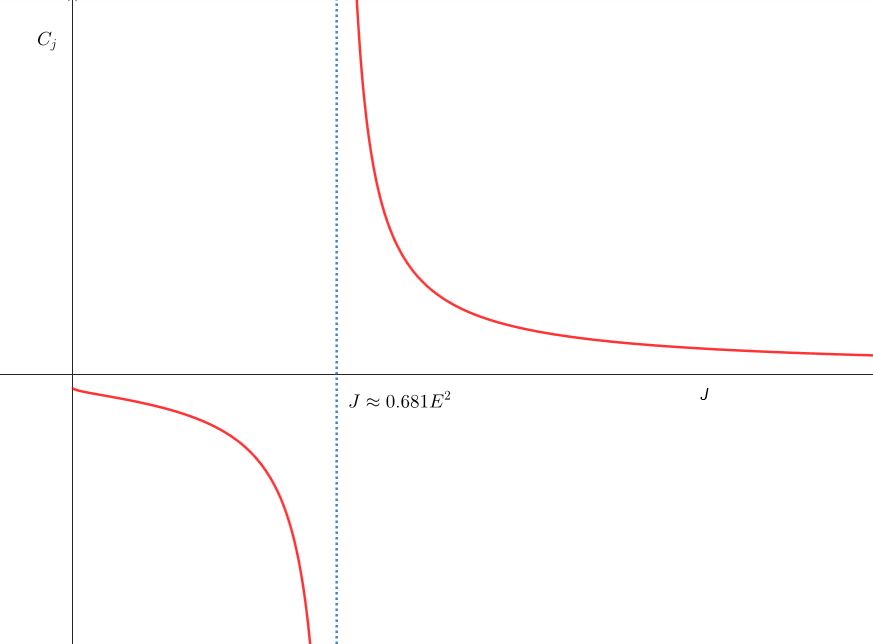
\includegraphics[scale=0.4]{immagini/kerr_heat_capacity.png}
    \caption{Calore specifico $C_J$ a $E=\cost$ per il buco nero di Kerr secondo eq. \ref{eq.calore_specifico_kerr}-\ref{eq.entropia_kerr_funzione_di_EJ}. Al valore $J=0$ si ottiene il risultato per Schwarzschild.}
    \label{fig.kerr_heat_capacity}
\end{figure}

Come noto dalla termodinamica, la trasformazione di Legendre permette di passare da un potenziale termodinamico ad un altro. L'energia libera di Gibbs è, per esempio:
\begin{equation}
    G(T, \Omega_H) = E - TS - \Omega_H J = \frac{1}{2}E
    \label{eq.en_libera_gibbs_ker}
\end{equation}
$G$ è continua alla discontinuità di $C_J$ e anche i suoi gradienti:
\begin{align*}
    \frac{\partial G}{\partial T}\Big|_{\Omega_H} && \frac{\partial G}{\partial \Omega_H}\Big|_T
\end{align*}
sono continui. Questo ci permette di dire che il fenomeno che avviene al valore critico $\frac{J^2}{E^4}\approx 0.464$ è una transizione di fase di II specie\footnote{Si ricorda che la transizione di fase di II specie implica la continuità di $G$ e delle sue derivate prima, ma la discontinuità delle seconde ovvero del calore specifico. Non c'è calore latente che invece contraddistingue le transizioni di I specie.}.
Si può fare un diagramma di fase (usando le espressioni delle derivate $\partial E/\partial S$ e $\partial E/\partial J$ prima calcolate):
\begin{equation}
    \frac{\Omega_H}{T} = \frac{\pi J}{S( \frac{1}{8\pi} - \frac{\pi J^2}{2S^2})}
    \label{eq.kerr_diagramma_fase}
\end{equation}
Se usiamo eq. \ref{eq.entropia_kerr_funzione_di_EJ} per esprimere $S$ e $J\approx 0.681E^2$, al valore critico si ha allora $\frac{\Omega_H}{T}\approx 5.843$. Il grafico di fase è mostrato in fig. \ref{fig.kerr_diagramma_fase}.
\begin{figure}
    \centering
    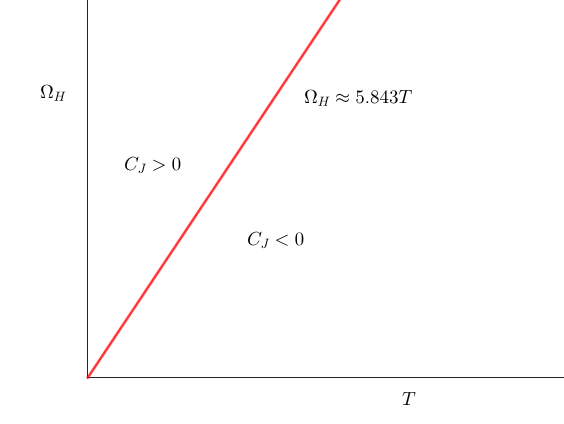
\includegraphics[scale=0.5]{immagini/kerr_diagramma_fase.png}
    \caption{Diagramma di fase per il buco nero di Kerr. In rosso il valore critico ottenuto da eq. \ref{eq.kerr_diagramma_fase} con $J\approx 0.681 E^2$.}
    \label{fig.kerr_diagramma_fase}
\end{figure}
La capacità termica $C_J$ ci permette di distinguere due differenti comportamenti del sistema:
\begin{itemize}
    \item $C_J < 0$: per un aumento di temperatura $\Delta T$, la massa del buco nero diminuisce e allora irradia di più, perdendo ancora più energia ecc.; il sistema è instabile e decade.
    \item $C_J > 0$: il buco nero può stare all'equilibrio termico con la radiazione.
\end{itemize}
\subsection{Termodinamica del buco nero di Schwarzschild-Tangherlini}
La soluzione di Schwarzschild-Tangherlini generalizza Schwarzschild ad una dimensione generica $d$ ed è descritta dalla metrica:
\begin{equation}
    ds^2 = - \left( 1 - \frac{\mu}{r^{d-3}}\right) dt^2 + \frac{dr^2}{1 - \frac{\mu}{r^{d-3}}} + r^2d\Omega_{d-2}^2
    \label{eq.schwarz_tangherlini}
\end{equation}
Con $d\Omega_{d-2}^2$ standard la metrica sulla $(d-2)$-sfera.

Per primo si calcola la temperatura di Hawking. Eseguiamo una rotazione di Wick $t \mapsto i\tau$:
\begin{equation*}
    ds^2 = \left( 1 - \frac{\mu}{r^{d-3}}\right) d\tau^2 + \frac{dr^2}{1 - \frac{\mu}{r^{d-3}}} + r^2d\Omega_{d-2}^2
\end{equation*}
La metrica è singolare in $r = \mu^{\frac{1}{d-3}} =: r_H$. Definiamo in analogia a quanto fatto per Schwarzschild:
\begin{equation*}
    \frac{x^2}{A} = r - r_H
\end{equation*}
con $A$ una costante opportuna da determinare. Segue che $dr = \frac{2x}{A}dx$.
Calcoliamo il termine che genera la singolarità nel limite $r \rightarrow r_H$:
\begin{align*}
    1 - \frac{\mu}{r^{d-3}} &= \left( 1 - \frac{\mu}{r^{d-3}}\right)\Big|_{r=r_H} + (d-3)\frac{\mu}{r^{d-2}}\Big|_{r=r_H}(r-r_H) + \dots \\
    &= (d-3)\frac{\mu}{\mu^{\frac{d-2}{d-3}}} + \dots= (d-3)\mu^{- \frac{1}{d-3}}\frac{x^2}{A} + \dots
\end{align*}
Chiamiamo per semplicità $B= (d-3)\mu^{- \frac{1}{d-3}} $. La metrica nel limite vicino alla singolarità è quindi:
\begin{align*}
    ds^2 &= \frac{B}{A^2}x^2d\tau^2 + \frac{4x^2}{A^2}\frac{A}{Bx^2}dx^2 + r_H^2d\Omega_{d-2}^2 \\
    &=\frac{B}{A^2}x^2d\tau^2 + \frac{4}{AB}dx^2 + r_H^2d\Omega_{d-2}^2
\end{align*}
A questo punto se scegliamo la costante iniziale come:
\begin{equation*}
    A = \frac{4}{B} = \frac{4}{(d-3)\mu^{-\frac{1}{d-3}}}
\end{equation*}
la metrica diventa:
\begin{equation*}
    ds^2 = \frac{B^2}{4}x^2d\tau^2 + dx^2 + M^2d\Omega_{d-2}^2 = \kappa^2 x^2 d\tau^2 + dx^2 + r_H^2d\Omega_{d-2}^2
\end{equation*}
che è un piano in $E_d$ in coordinate polari se identifichiamo $\tau \sim \tau + \frac{2\pi}{\kappa}$ così da non avere singolarità conica.  La temperatura è l'inverso del periodo del tempo euclideo quindi si trova:
\begin{equation}
    T = \frac{\kappa}{2\pi} = \frac{B}{4\pi} = \frac{(d-3)}{4\pi}\mu^{-\frac{1}{d-3}}
    \label{eq.temp_schwarz_tangherlini}
\end{equation}

Come passo successivo allo studio della termodinamica di questo buco nero, calcoliamo l'entropia di Bekenstein-Hawking secondo eq. \ref{eq.entropia_beken_hawking}. Serve calcolare l'area dell'orizzonte degli eventi: la metrica indotta sull'orizzonte è:
\begin{equation*}
    d\sigma^2 = r_H^2d\Omega_{d-2}^2 = r_H^2( \alpha_1 d\theta_1^2 + \alpha_2 d\theta_2^2 + \dots + \alpha_{d-2}d\theta_{d-2}^2)
\end{equation*}
con $\alpha_i(\bm\theta)$ i coefficienti che appaiono nella scrittura della metrica sulla $(d-2)$-sfera, funzioni dei vari angoli. Il determinante è pari a (osservando bene che $r_H$ è fattore comune a tutti i termini):
\begin{equation}
    \sigma = r_H^{2(d-2)}\prod_{i=1}^{d-2}\alpha_i(\bm\theta) = r_H^{2(d-2)}\det S^{d-2}
    \label{eq.sigma_indotta_scha_tang}
\end{equation}
L'area dell'orizzonte:
\begin{equation*}
    A = \int \sqrt{\sigma}d\Omega_{d-2} =  r_H^{d-2} \int\sqrt{\det S^{d-2}}d\theta_1\dots d\theta_{d-2} = r_{H}^{d-2}V(S^{d-2})
\end{equation*}
Se chiamiamo $V(S^{d-2})$ il volume della $(d-2)$-sfera. Quindi l'entropia:
\begin{equation}
    S = \frac{A}{4G} = \frac{r_H^{d-2}V(S^{d-2})}{4G} = \frac{V(S^{d-2})}{4G}\mu^{\frac{d-2}{d-3}}
    \label{eq.entropia_schwarz_tangherlini}
\end{equation}

Calcoliamo ora la massa di Komar associata al vettore di Killing $\xi = \partial_t$:
\begin{equation*}
    Q = \frac{c}{16\pi G} \oint_{\partial V} dS_{\mu\nu} \nabla^\mu \xi^\nu
\end{equation*}
con $c$ la costante da determinare e $dS_{\mu\nu}$ l'elemento di metrica indotta su $\partial V$, orientato. Consideriamo $\partial V$ come l'intersezione tra l'ipersuperficie $\Sigma$ dei tempi costanti e l'ipersuperficie $r= \textrm{cost.}$  Introduciamo il vettore normale di tipo tempo:
\begin{equation*}
    u = N^{-1}\partial_t \quad \textrm{ dove } \quad N = \sqrt{1 - \frac{\mu}{r^{d-3}}}
\end{equation*}
infatti $<u,u> = N^{-2} g_{tt} = -1$ e $< u, \partial_i> = 0$ per $i=1, \dots, d-2$.
Il vettore normale di tipo spazio possiamo definirlo come:
\begin{equation*}
    v = N\partial_r
\end{equation*}
che similmente a sopra soddisfa $<v,v> = 1$, $<v, \theta_i> = 0$ per $i= 1, \dots, d-2$. La misura indotta e orientata su $\partial V$ risulta:
\begin{equation*}
    dS^{\mu\nu} = (v^\mu u^\nu - u^\mu v^\nu)\sqrt{\sigma}d\theta_1\dots d\theta_{d-2}
\end{equation*}
con $\sigma$ di eq. \ref{eq.sigma_indotta_scha_tang}. Siccome vale in generale:
\begin{equation*}
    dS^{\mu\nu}\nabla_\mu\xi_\nu = \sqrt{\sigma}d\theta_1\dots d\theta_{d-2} ( - 2v^\nu u^\mu)\nabla_\mu \xi_\nu
\end{equation*}
 e $dS^{\mu\nu} = - dS^{\nu\mu}$, elaboriamo un attimo l'integrale di Komar ed eseguiamo i calcoli:
\begin{align*}
    Q &= \frac{c}{16\pi G}\oint_{\partial V} dS^{\sigma\rho}g_{\mu\sigma}g_{\nu\rho}g^{\alpha\mu}\nabla_\alpha \xi^\nu = - \frac{c}{16\pi G} \oint_{\partial V}dS^{\rho\sigma}\delta^\alpha_\sigma g_{\nu\rho}\nabla_\alpha \xi^\nu \\
     &=  \frac{c r^{d-2}}{8\pi G} \oint_{\partial V} v^\sigma u^\rho g_{\nu\rho}\nabla_\sigma \xi^\nu \sqrt{\det S^{d-2}}d\theta_1 \dots d\theta_{d-2} \\
    &=  \frac{c r^{d-2}}{8\pi G} \oint_{\partial V} v^r u^t g_{\nu r}\nabla_r \xi^\nu \sqrt{\det S^{d-2}}d\theta_1 \dots d\theta_{d-2} \\
    &= \frac{c r^{d-2}}{8\pi G} \oint_{\partial V} g_{\nu t}\nabla_r \xi^\nu \sqrt{\det S^{d-2}}d\theta_1 \dots d\theta_{d-2}
\end{align*}
Si deve solamente calcolare $\nabla_r \xi^t = \partial_r(\partial_t) + \tensor{\Gamma}{^t_{\lambda r}}\xi^\lambda = \tensor{\Gamma}{^t_{rt}}$. Il simbolo di Christoffel si determina da eq. \ref{eq.connlevicivita}:
\begin{equation*}
    \tensor{\Gamma}{^t_{rt}} = \frac{1}{2}g^{tt}g_{tt,r} = - \frac{1}{2}g^{tt}\partial_r\left( 1 - \frac{\mu}{r^{d-3}}\right) = - \frac{g^{tt}}{2}(d-3)\frac{\mu}{r^{d-2}}
\end{equation*}
allora:
\begin{equation*}
    Q = -\frac{c r^{d-2}}{16\pi G}\oint_{\partial V} g_{tt}g^{tt}(d-3)\frac{\mu}{r^{d-2}}\sqrt{\det S^{d-2}}d\theta_1 \dots d\theta_{d-2}
\end{equation*}
La massa (o energia, quantità conservata con il vettore di Killing $\partial_t$) è pertanto\footnote{Scelto $c=-1$. La definizione generale di questa quantità conservata pone come prefattore $-\frac{1}{8\pi G}$ che se usata qui fin dall'inizio ci farebbe ottenere un valore della massa/energia positivo.}:
\begin{equation}
    M = \frac{d-3}{16 \pi G} V(S^{d-2})\mu
    \label{eq.massa_schwarz_tangherlini}
\end{equation}
Si può verificare che eq. \ref{eq.temp_schwarz_tangherlini},
 \ref{eq.entropia_schwarz_tangherlini} e \ref{eq.massa_schwarz_tangherlini} soddisfano:
 \begin{equation*}
     dM = TdS
 \end{equation*}

 Da eq. \ref{eq.entropia_schwarz_tangherlini} possiamo esplicitare $\mu(S)$:
\begin{equation*}
     \mu(S) = (4S)^{\frac{d-3}{d-2}}\left( \frac{V(S^{d-2})}{G}\right)^{- \frac{d-3}{d-2}}
 \end{equation*}
così da sostituire in eq. \ref{eq.massa_schwarz_tangherlini} e ottenere:
\begin{equation}
    M(S) = \frac{d-3}{16\pi}\left( \frac{V(S^{d-2})}{G}\right)^{\frac{1}{d-2}}(4S)^{\frac{d-3}{d-2}}
    \label{eq.rel_fondam_massa_schwarz_tangh}
\end{equation}
oppure sostituendo in eq. \ref{eq.temp_schwarz_tangherlini}:
\begin{equation}
    T(S)= \frac{d-3}{4\pi}(4S)^{-\frac{1}{d-2}} \left( \frac{V(S^{d-2})}{G}\right)^{\frac{1}{d-2}}
    \label{eq.rel_fondam_temper_schwarz_tangh}
\end{equation}
Per eq. \ref{eq.rel_fondam_massa_schwarz_tangh} vale la relazione di Eulero:
\begin{equation*}
    M(\lambda S) = \lambda^{\frac{d-3}{d-2}}M(S)
\end{equation*}
Così possiamo calcolare, con l'obiettivo di ottenere la formula di Smarr:
\begin{align*}
    \frac{\partial M(\lambda S)}{\partial \lambda} &= S \frac{\partial M}{\partial(\lambda S)}= \frac{S}{\lambda}\frac{\partial M}{\partial S} =\frac{S(d-3)}{\lambda(d-2)}\left[\frac{d-3}{16\pi}\left(\frac{V(S^{d-2})}{G}\right)^{\frac{1}{d-2}}4^{\frac{d-3}{d-2}}S^{- \frac{1}{d-2}}\right] \\
    &= \frac{S(d-3)}{\lambda(d-2)}\left[\frac{d-3}{4\pi}\left(\frac{V(S^{d-2})}{G}\right)^{\frac{1}{d-2}}(4S)^{- \frac{1}{d-2}}\right] = \frac{S(d-3)}{\lambda(d-2)} T
\end{align*}
e anche:
\begin{equation*}
    \frac{\partial M(\lambda S)}{\partial \lambda} = \frac{\partial}{\partial \lambda}\left( \lambda^{\frac{d-3}{d-2}}\right)M(S) = \frac{d-3}{d-2}\lambda^{\frac{d-3}{d-2}-1}M(S)
\end{equation*}
Uguagliando queste due e mettendo poi $\lambda = 1$, si trova la formula di Smarr:
\begin{equation*}
    M(S) = TS
\end{equation*}

Possiamo ora calcolare la capacità termica e discuterne la stabilità. Se riarrangiamo eq. \ref{eq.temp_schwarz_tangherlini} per isolare $\mu(T)$:
\begin{equation*}
    \mu(T) = \left( \frac{d-3}{4\pi}V(S^{d-2})\right)^{d-3}T^{-(d-3)}
\end{equation*}
si ottiene sostituendo in eq. \ref{eq.massa_schwarz_tangherlini}:
\begin{equation*}
    M(T) = \frac{1}{4G}\left( \frac{d-3}{4\pi}V(S^{d-2})\right)^{d-2}T^{-(d-3)}
\end{equation*}
Dunque la capacità termica:
\begin{equation}
    C =  \frac{\partial M}{\partial T} = - \frac{d-3}{4G}\left( \frac{d-3}{4\pi}V(S^{d-2})\right)^{d-2}T^{-(d-2)} = - (d-3) \frac{M}{T^{d-2}} \label{eq.cap_termica_schwarz_tangh}
\end{equation}
Possiamo discuterne la stabilità:
\begin{itemize}
    \item $d=2$ allora $C = \frac{1}{4G}= \textrm{cost.}$ . Il buco nero può stare in equilibrio termico con la radiazione.
    \item $d= 3$ allora $C = 0$.
    \item $d > 3$ allora $C \propto - T^{-(d-2)}$. La capacità termica è sempre negativa con tendenza a zero per $T \rightarrow + \infty$. Non presenta estremi.  Il buco nero diventa più caldo quando irradia energia e pertanto decade in fretta sotto radiazione di Hawking.
\end{itemize}
Osserviamo che per $d=4$ si ottiene lo stesso risultato della capacità termica di Kerr con $J=0$.
\section{Buco nero di BTZ}
Consideriamo una gravità in 3-dim. con costante cosmologica $\Lambda < 0$. La teoria è descritta dall'azione:
\begin{equation*}
    I= \frac{1}{16\pi G} \int d^3x \sqrt{-g}( R - 2\Lambda )   
\end{equation*}
dove $\Lambda = - \frac{1}{l^2}$ e le equazioni del moto sono:
\begin{equation*}
    G_{\mu\nu} + \Lambda g_{\mu\nu} = 0
\end{equation*}
Come visto, uno spazio del genere è uno spazio di Einstein. Poiché siamo in dimensione 3, il tensore di Weyl è nullo, eq. \ref{eq.tensore_weyl}, e perciò lo spazio è anche a curvatura costante. Siccome uno spazio di Einstein a curvatura costante è di Minkowski, de Sitter o Anti-de Sitter, questa soluzione è \textbf{localmente $AdS_3$}.

La soluzione di \textbf{Banados-Teitelboim-Zanelli} \cite{btz} è descritta dalla metrica:
\begin{equation}
    ds^2 = - N^2dt^2 + \frac{dr^2}{N^2} + r^2(d\phi + N^\phi dt)^2
    \label{eq.metrica_btz}
\end{equation}
dove:
\begin{align*}
    N = \sqrt{-8GM + \frac{r^2}{l^2} + \frac{16 G^2 J^2}{r^2}} && N^\phi = - \frac{4GJ}{r^2}
\end{align*}
La metrica è singolare in $r= r_\pm$ definiti:
\begin{equation*}
    r_\pm^2 = 4GMl^2 \left[1 + \pm \sqrt{1 - \left(\frac{J}{Ml}\right)^2}\right]
\end{equation*}
Si deve avere $|J|\leq Ml$ così $r_+$ è l'orizzonte degli eventi e $r_-$ è quello di Cauchy. Per $|J| = Ml$ il buco nero è estremo e $r_+=r_-$.

Si dimostra che il buco nero di BTZ ha un'ergosfera al raggio:
\begin{equation}
    r_{erg}= (r_+^2 + r_-^2)^{1/2}
\end{equation}
corrispondente a richiedere $g_{tt} = 0$. Si dimostra che $r=r_+$ è un orizzonte di Killing per
\begin{equation*}
    \chi = \partial_v - N^\phi(r_+)d\Tilde{\phi}
\end{equation*}
dove $v, \Tilde{\phi}$ sono le coordinate di tipo Eddington-Finkelstein:
\begin{align*}
    dv = dt + \frac{dr}{N^2} && d\Tilde{\phi} = d\phi - \frac{N^\phi}{N^2}dr
\end{align*}
La gravità superficiale, calcolata da eq. \ref{eq.gravità_sup_quadrata}, risulta:
\begin{equation}
    \kappa = \frac{r_+^2 -r_-^2}{l^2r_+}
    \label{eq.grav_sup_btz}
\end{equation}
I valori $M, J$ sono massa e momento angolare come cariche associate ai vettori di Killing $\partial_t, \partial_\phi$ rispettivamente. Se si vuole eseguire il calcolo del loro integrale di Komar, bisogna considerare che diverge e serve pertanto sottrarre un background di $J=0$, $M=0$ rispettivamente.
L'entropia associata a questo buco nero è:
\begin{equation*}
    S = \frac{A_H}{4G} = \frac{2\pi r_+}{4G}
\end{equation*}

Il buco nero ha una rotazione. Gli osservatori localmente non rotanti hanno vettori tangenti:
\begin{equation*}
    \partial_t - N^\phi\partial_\phi
\end{equation*}
ovvero:
\begin{align*}
    <\partial_t - N^\phi\partial_\phi, \partial_\phi > &= 0 \\
    <\partial_t - N^\phi\partial_\phi, \partial_r > &= 0
\end{align*}
Questi però ruotano rispetto osservatori con vettori tangenti  $\partial_t$ ovvero degli osservatori localmente non rotanti a infinito o anche detti osservatori statici a infinito. La velocità angolare della rotazione è $\Omega = -N^\phi$ e pertanto la velocità di rotazione dell'orizzonte:
\begin{equation}
    \Omega_H = - N^\phi\Big|_{r=r_+} = \frac{4GJ}{r_+^2}
\end{equation}
Questo può essere mostrato considerando che gli osservatori localmente non rotanti sono tali che $\phi + N^\phi t = \cost$ lungo la linea di mondo\footnote{Questo deriva da $(\partial_t - N^\phi\partial_\phi)(\phi + N^\phi t) = 0$ con $\partial_t - N^\phi\partial_\phi$ che come detto è il loro vettore tangente alla linea di mondo.}. Dunque:
\begin{equation*}
    \phi = \cost - N^\phi t = \cost + \Omega t
\end{equation*}

La temperatura del buco nero può essere determinata dalla gravità superficiale di eq. \ref{eq.grav_sup_btz} in eq. \ref{eq.temperatura_hawking}. Si può esplicitamente fare il calcolo alternativo usando la sezione pseudoeuclidea, quindi facendo la rotazione di Wick $t = i\tau$:
\begin{equation*}
    ds_E^2= N^2d\tau^2 + \frac{dr^2}{N^2} + r^2(d\phi +iN^\phi d\tau)^2
\end{equation*}
Vicino a $r=r_+$ si ha lo sviluppo:
\begin{equation*}
    N^2 = N^2(r_+) + \frac{dN^2}{dr}\Big|_{r_+}(r-r_+) + o((r-r_+))
\end{equation*}
Facendo una semplice sostituzione $\rho^2 = r-r_+$, in questo limite:
\begin{equation*}
    ds_E^2 = \frac{4}{\frac{dN^2}{dr}\Big|_{r_+}}\left[ d\rho^2 + \left(\frac{dN^2}{dr}\Big|_{r_+}\right)^2\frac{\rho^2}{4} d\tau^2\right] + r_+^2(d\phi - i\Omega_H d\tau)^2
\end{equation*}
Quindi non si hanno singolarità coniche se $\tau \sim \tau + \frac{2\pi}{\frac{1}{2}\frac{dN^2}{dr}}\Big|_{r_+}$. Il calcolo della derivata è più semplice se usiamo la forma $N^2= \frac{1}{r^2l^2}(r^2-r_+^2)(r^2-r_-^2)$, così si ottiene la temperatura:
\begin{equation}
    T_H = \frac{r_+^2 - r_-^2}{2\pi l^2r_+}
    \label{eq.temp_btz}
\end{equation}
Nel caso di buco nero estremo, $r_+ = r_-$ e $T_H=0$.

La relazione fondamentale termodinamica:
\begin{equation}
    M(S,J) = \frac{G S^2}{2\pi^2l^2} + \frac{\pi^2 J^2}{2GS^2}
    \label{eq.rel_fondam_btz}
\end{equation}
fornisce correttamente $T = \frac{\partial M}{\partial S}$ e $\Omega_H = \frac{\partial M}{\partial J}$. La relazione di Eulero $M(\lambda S, \lambda^2 J)=\lambda^2 M(S,J)$ determina la formula di Smarr:
\begin{equation}
    M = \frac{1}{2}TS + \Omega_H J
    \label{eq.smarr_btz}
\end{equation}
Queste sono le proprietà generali termodinamiche del buco nero di BTZ.

Discutiamo ora la geometria globale del buco nero. Come già detto, questa soluzione è localmente $AdS_3$, quindi ogni intorno è isomorfo ad anti-de Sitter. Verrà mostrato come risultato finale che il buco nero BTZ è invece uno spazio quoziente di $AdS_3$\footnote{Lo spaziotempo massimale semplicemente connesso a curvatura costante negativa è lo spazio di ricoprimento universale $\Tilde{AdS}$ di anti-de Sitter. Per questo motivo scriveremo BTZ come spazio quoziente di $\Tilde{AdS}$  per un qualche gruppo di isometrie.}, corrispondente ad unire appropriatamente queste collezioni di intorni.
Tra le varie cose, questo vuol dire che la sua struttura a $r=\infty$ sia asintoticamente anti-de Sitter invece che asintoticamente piatta come avviene per Kerr.

Ricordiamo che $AdS_3$ è l'ipersuperficie di $\mathbb R^{2+2}$ definita da:
\begin{equation}
    X_1^2 + X_2^2 - T_1^2 -T_2^2 = -l^2
    \label{eq.ipersup_ads3}
\end{equation}
con metrica:
\begin{equation*}
    ds^2 = dX_1^2 + dX_2^2 - dT_1^2 - dT_2^2
\end{equation*}
e gruppo di isometrie $SO(2,2)$. La definizione dell'ipersuperficie può essere riassunta in forma di matrice con:
\begin{equation*}
    X = \frac{1}{l}\begin{pmatrix}
        T_1 + X_1 & T_2 + X_2 \\
        -T_2 + X_2 & T_1 - X_1
    \end{pmatrix}
\end{equation*}
così l'ipersuperficie eq. \ref{eq.ipersup_ads3} corrisponde a $\det X = 1$ e $X \in SL(2,\mathbb R)$.
Possiamo rappresentare le isometrie come gli elementi del gruppo:
\begin{equation*}
    SL(2,\mathbb R) \times \faktor{SL(2,\mathbb R)}{\mathbb Z_2} \approx SO(2,2)
\end{equation*}
Le due coppie di $SL(2,\mathbb R)$ agiscono come moltiplicazione destra e sinistra su un elemento $X$:
\begin{equation*}
    X \mapsto \rho_L X \rho_R
\end{equation*}
e vale inoltre $(\rho_L, \rho_R) = (-\rho_L, - \rho_R)$. Questo per quanto riguarda $AdS_3$.

Per $r \geq r_+$ parametrizziamo l'ipersuperficie eq. \ref{eq.ipersup_ads3} tramite:
\begin{align*}
    X_1 &= l\sqrt{\alpha}\sinh(\frac{r_+}{l}\phi - \frac{r_-}{l^2}t) \\
    X_2 &= l\sqrt{\alpha - 1}\cosh( \frac{r_+}{l^2}t - \frac{r_-}{l}\phi) \\
    T_1 &= l\sqrt{\alpha}\cosh(\frac{r_+}{l}\phi - \frac{r_-}{l^2}t)\\
    T_2 &= l\sqrt{\alpha - 1} \sinh(\frac{r_+}{l^2}t - \frac{r_-}{l}\phi)
\end{align*}
dove $\phi, t \in \mathbb R$ su $AdS_3$ e 
\begin{equation*}
    \alpha = \frac{r^2 - r_-^2}{r_+^2 - r_-^2}
\end{equation*}
Con questa parametrizzazione possiamo ricondurci alla regione $r\geq r_+ $ di BTZ se però identifichiamo $\phi \textrm{ mod } 2\pi$ . La metrica indotta coincide con quella di BTZ. Per le altre regioni di BTZ servono differenti parametrizzazioni (vedi \cite{btz}), corrispondenti ad altre zone del diagramma di Penrose.

Questa identificazione di $\phi$ con $\phi \textrm{ mod } 2\pi$ è un'isometria di $AdS_3$ (è un boost nei piani $X_1$-$T_1$ e $X_2$-$T_2$) a cui corrispondono gli elementi di $(\rho_L, \rho_R)$ con:
\begin{equation*}
    \rho_L = \begin{pmatrix}
        e^{\pi(r_+-r_-)/l} & 0 \\
        0 & e^{-\pi(r_+-r_-)/l}
    \end{pmatrix}
\end{equation*}
\begin{equation*}
    \rho_R = \begin{pmatrix}
        e^{\pi(r_+ + r_-)/l} & 0 \\
        0 & e^{-\pi(r_+ + r_-)/l}
    \end{pmatrix}
\end{equation*}
SI può quindi mostrare che:
\begin{equation*}
    BTZ = \faktor{AdS_3}{<(\rho_L,\rho_R)>}
\end{equation*}
dove $<(\rho_L,\rho_R)>$ è il gruppo discreto generato dagli elementi $(\rho_L,\rho_R)$.

Questo risultato è importante in quanto $AdS_3$ è una varietà estremamente semplice e virtualmente priva di struttura; tuttavia con le opportune identificazioni, si può convertire in uno spaziotempo (BTZ) con proprietà molto simili a Kerr $(3+1)$-dimensionale. In tutto ciò BTZ rimane uno spaziotempo a curvatura costante e inoltre, come verrà visto in \S\ref{para.chern}, la gravità 3-dimensionale è esprimibile come una teoria di gauge che può essere quantizzata.
\chapter{Formalismo di Ernst}
In questo capitolo verrà visto e introdotto un sistema estremamente efficace per la risoluzione delle equazioni di Einstein e la generazione di nuove soluzioni; il formalismo di Ernst. Tramite questo metodo, che introduce dei potenziali omonimi soddisfacenti l'equazione di Ernst, le soluzioni per uno spaziotempo assisimmetrico e stazionario saranno più facilmente ottenibili rispetto l'integrazione diretta delle equazioni di Einstein. Come verrà mostrato, questo formalismo è del tutto equivalente alle equazioni di campo della relatività generale, guadagnando però in \virgolette{semplicità}; basti pensare che per ottenere direttamente la soluzione di Kerr sono stati necessari 50 anni di tentativi; tramite questo sistema delle soluzioni molto più complesse e che combinano soluzioni esatte già note, saranno ricavabili.

\section{Equazioni e potenziali di Ernst}
Risolviamo le equazioni di Einstein richiedendo che lo spaziotempo possieda i vettori di Killing $\xi = \partial_t$ e $\eta = \partial_\phi$ tali che $[\xi, \eta] = 0$, quindi che sia stazionario e assisimmetrico. Questo tipo di soluzioni sono utili per descrivere buchi neri rotanti, stelle e in generale corpi assisimmetrici in rotazione, ma non per soluzioni cosmologiche visto che in questo caso la stazionarietà cade.

Si ha una simmetria del tipo:
\begin{equation*}
    \left\{\begin{array}{c}
         t\mapsto -t \\
         \phi \mapsto -\phi
     \end{array}\right.
\end{equation*}
quindi la metrica (4-dim.) avrà dipendenza solo dalle altre componenti:
\begin{equation*}
    g_{\mu\nu}=g_{\mu\nu}(x_1,x_2) \qquad g_{it}=g_{i\phi} = 0 ,\quad i=1,2
\end{equation*}
perciò la forma più generale è:
\begin{equation}
    ds^2 = g_{00}dt^2 + 2g_{03}dtd\phi + g_{33}d\phi^2 + g_{ij}dx^i dx^j
    \label{eq.metrica_stazio_assisim_generale}
\end{equation}
Il tensore di Weyl è nullo in 2-dim (relativamente a $x_1, x_2$) perciò è possibile fare il cambio di coordinate:
\begin{equation*}
    g_{ij}dx^i dx^j \rightarrow g_{22}\left[ (d\bm{x}^1)^2 + (d\bm{x}^2)^2\right]
\end{equation*}
Siccome il sistema gode di simmetria cilindrica, risulta conveniente esprimere $(x_1, x_2) = (\rho, z)$ e ci riduciamo ad un sistema con incognite che scriviamo nella forma:
\begin{align*}
         g_{00} = -f \qquad& g_{03} =f\omega  \\
         g_{33} = \frac{\alpha^2}{f} \qquad& g_{22} = \frac{e^{2\gamma}}{f} 
\end{align*}
così che la metrica diventa:
\begin{equation}
    ds^2 = - f(\rho,z) \left[ dt - \omega(\rho, z) d\phi\right]^2 + \frac{1}{f(\rho,z)}\left[ e^{2\gamma(\rho, z)}(d\rho^2 + dz^2) + \alpha^2(\rho) d\phi^2 \right]
    \label{eq.metrica_stazio_assisim_cilindriche}
\end{equation}
Questa è la più generica metrica stazionaria, assisimmetrica in coordinate cilindriche. Come si vedrà fra poco, si può tranquillamente porre $\alpha(\rho) = \rho$ così che eq. \ref{eq.metrica_stazio_assisim_cilindriche} viene chiamata \textbf{metrica di Lewis-Weyl-Papapetrou} (LWP).

Possiamo risolvere le equazioni in un sistema di Einstein-Maxwell con azione che scriviamo, diversamente da eq. \ref{eq.azione_einstein_maxwell}, nella forma:
\begin{equation*}
    S = \frac{1}{16\pi G}\int d^4x \sqrt{-g} \left( R - F_ {\mu\nu} F^{\mu\nu} \right)
\end{equation*}
La variazione porta alle equazioni del moto:
\begin{align}
    \tensor{EE}{^\mu_\nu} :=& \quad \tensor{R}{^\mu_\nu} - \frac{1}{2}\delta^\mu_\nu R = 2 \tensor{T}{^\mu_\nu} \label{eq.ee}\\
   ME^\nu :=& \quad \nabla_\mu F^{\mu\nu} = 0 \label{eq.me}
\end{align}
Il tensore di gauge lo scegliamo nella forma che rispetta le simmetrie della metrica:
\begin{equation}
    A_\mu = \left( A_t(\rho,z), 0,0, A_\phi(\rho,z)\right)
    \label{eq.pot_gauge_cilindrico}
\end{equation}

Ora verranno risolte le varie equazioni per ottenere i potenziali di Ernst e la rispettiva equazione.
\begin{itemize}
\item $\tensor{EE}{^\rho_\rho} + \tensor{EE}{^z_z}$ implica:
\begin{equation*}
    0 = \frac{f}{e^{2\gamma}\alpha}\left( \partial_{\rho\rho}\alpha + \partial_z \alpha \right)
\end{equation*}
Questa equazione è disaccoppiata dalle altre e il fatto che $\Lambda = 0$ rende possibile lo zero al membro di sinistra. Questa equazione ci permette di porre $\alpha = \rho$, come prima accennato.
    \item $ME^\phi$ implica:
\begin{align*}
    \frac{f}{e^{2\gamma}}&\left[\frac{\partial_\rho f}{\rho^2}(\partial_\rho A_\phi + \omega\partial_\rho A_t) + \frac{\partial_z f}{\rho^2}(\partial_z A_\phi + \omega\partial_z A_t)  - \frac{f}{\rho^3}(\partial_\rho A_\phi +\omega\partial_\rho A_t) + \right. \\ 
&\left. + \frac{f}{\rho^2}(\partial_{\rho\rho}A_\phi + \partial_{zz}A_\phi + \omega\partial_{\rho\rho} A_t + \omega\partial_{zz}A_t + \partial_\rho\omega\partial_\rho A_t + \partial_z \omega \partial_z A_t) \right]
\end{align*}
che possiamo scrivere come:
\begin{equation}
    - \frac{t}{e^{2\gamma}}\left[ \nabla\cdot \left( \frac{f}{\rho^2}(\nabla A_\phi + \omega \nabla A_t) \right)\right]
\label{eq.me_phi}
\end{equation}
Gli operatori $\nabla\cdot$ e $\nabla$ sono quelli usuali di una metrica piatta cilindrica $ds^2 = d\rho^2 + \rho^2d\phi^2 + dz^2$:
\begin{align*}
    \nabla f &= \partial_\rho f \hat{e}_\rho + \partial_z f \hat{e}_z \\
    \nabla\cdot A &= \frac{1}{\rho} A_\rho + \partial_\rho A_\rho + \partial_z A_z
\end{align*}
\item $ME^t$ implica:
\begin{equation}
    \nabla\cdot \left[ \frac{1}{f}\nabla A_t - \frac{f\omega}{\rho^2}(\nabla A_\phi + \omega \nabla A_t) \right] = 0
\label{eq.me_t}
\end{equation}
\item $\tensor{EE}{^\phi_t}$ implica:
\begin{equation}
    \nabla\cdot \left[ \frac{f^2}{\rho^2}\nabla\omega + \frac{f}{\rho^2}A_t (\nabla A_\phi + \omega \nabla A_t) \right] = 0
\label{eq.ee_phi_t}
\end{equation}
\item $\tensor{EE}{^t_\phi} - \tensor{EE}{^\phi_\phi}$ implica:
\begin{equation}
    f\nabla^2f = (\nabla f)^2 - \frac{f^4}{\rho^2}(\nabla\omega)^2 + 2f\left[(\nabla A_\phi)^2 + \frac{f^2}{\rho^2}(\nabla A_\phi + \omega \nabla A_t)^2 \right]
\label{eq.ee_tphi_phiphi}
\end{equation}
\end{itemize}
Queste ultime sono quattro equazioni in quattro incognite ($\omega, f, A_\phi, A_t$) e quindi il sistema è risolvibile. Non appare $\gamma$ in quanto agisce da seme della soluzione che solitamente viene preso a partire da altre soluzioni note; in questa maniere si possono generare continuamente nuove soluzioni dalle precedenti. La funzione $\gamma$ viene determinata da $\tensor{EE}{^\rho_z}$ che fornisce $\partial_\rho \gamma$ e $\partial_z \gamma$.

Dunque il procedimento è il seguente: si parte da una soluzione di $[f_0, \omega_0, A_{0t}, A_{0\phi}]$ che viene usata nell'equazione per $\gamma$ di prima; $\gamma$ è disaccoppiato dal sistema di quattro equazioni e quindi rimane invariato tra differenti soluzioni. Successivamente si risolve il sistema di equazioni per la nuova soluzione, controllando bene che le soluzioni finali siano effettivamente nuove e non di gauge.

Iniziamo ad eseguire i calcoli. Sfruttiamo il fatto che $\nabla \cdot (\frac{1}{\rho}\hat{e}_\phi \times \nabla h) = $ se $h$ è almeno $C^2$ .
Dall'eq. \ref{eq.me_phi} si può notare che conviene definire $\Tilde{A}_\phi$ tale che:
\begin{equation}
   \hat{e}_\phi \times \nabla\Tilde{A}_\phi = \frac{f}{\rho}(\nabla A_\phi + \omega \nabla A_t )
   \label{eq.potenziale_twisted}
\end{equation}
detto \textbf{potenziale twisted}. Così è direttamente soddisfatta l'equazione di Maxwell $\nabla\cdot(\frac{1}{\rho}\hat{e}_\phi \times \nabla\Tilde{A}_\phi )= 0$. Possiamo successivamente usare l'identità $\bm{v}\times(\bm{u}\times\bm{w}) = \bm{u}(\bm{v}\cdot\bm{w}) - \bm{w}(\bm{v}\cdot\bm{u})$ così:
\begin{equation*}
    \hat{e}_\phi \times (\hat{e}_\phi \times \nabla \Tilde{A}_\phi ) = - \nabla\Tilde{A}_\phi
\end{equation*}
e poiché
\begin{equation*}
    -\nabla\Tilde{A}_\phi = \frac{f}{\rho}\hat{e}_\phi \times \nabla A_\phi  + \frac{f}{\rho} \omega \hat{e}_\phi \times A_t \implies \frac{1}{\rho}\hat{e}_\phi \times \nabla A_\phi = - \left( f^{-1}\nabla \Tilde{A}_\phi + \frac{\omega}{\rho}\hat{e}_\phi \times \nabla A_t \right)
\end{equation*}
le eq. \ref{eq.me_phi}, \ref{eq.me_t} diventano:
\begin{align}
    \nabla\cdot\left[ f^{-1}\nabla \Tilde{A}_\phi + \frac{\omega}{\rho}\hat{e}_\phi \times \nabla A_t \right] = 0 \label{eq.me_phi_redone} \\
    \nabla\cdot\left[ f^{-1}\nabla A_t - \frac{\omega}{\rho}\hat{e}_\phi \times \nabla\Tilde{A}_\phi \right] = 0 \label{eq.me_t_redone}
\end{align}
\begin{definizione}
Definiamo il \textbf{potenziale di Ernst} complesso:
\begin{equation}
    \Phi = A_t + i\Tilde{A}_\phi
    \label{eq.potenziale_ernst_phi}
\end{equation}
\end{definizione}
Così eq. \ref{eq.me_phi_redone}, \ref{eq.me_t_redone} vengono riassunte in:
\begin{equation}
    \nabla\cdot\left[ f^{-1}\nabla\Phi + i\frac{\omega}{\rho}\hat{e}_\phi \times \nabla\Phi \right] = 0
    \label{eq.ernst_0}
\end{equation}

L'eq. \ref{eq.ee_phi_t} può essere riscritta come:
\begin{equation*}
    \nabla\cdot\left[ \frac{f^2}{\rho}\nabla\omega + \frac{2}{f}\hat{e}_\phi \times \Im{\Phi^*\nabla\Phi}\right] = 0
\end{equation*}
dove $\Im{\Phi^*\nabla\Phi} = - \Tilde{A}_\phi\nabla A_t + A_t\nabla\Tilde{A}_\phi$. In analogia al caso elettrico possiamo definire $h$ tale che:
\begin{equation}
    \hat{e}_\phi \times \nabla h = - \frac{f^2}{\rho^2}\nabla\omega  - 2\hat{e}_\phi\times \Im{\Phi^*\nabla\Phi}
\end{equation}
In questo modo $-\nabla h = \hat{e}_\phi\times(\hat{e}_\phi \times \nabla h) = - \frac{f^2}{\rho^2}\hat{e}_\phi\times\nabla\omega - 2\hat{e}_\phi\times(\hat{e}_\phi \times \Im{\Phi^*\nabla\Phi})$ da cui segue:
\begin{equation*}
    \hat{e}_\phi \times \nabla\omega = f^{-1}\left[ \nabla h +2\Im{\Phi^*\nabla\Phi}\right]
\end{equation*}
Tutto ciò permette di riscrivere eq. \ref{eq.ee_phi_t} come:
\begin{equation}
    \nabla\cdot\left[ f^{-2}\nabla h + \frac{2}{f^2}\Im{\Phi^*\nabla\Phi}\right]
    \label{eq.ernst_3}
\end{equation}
L'eq. \ref{eq.ee_tphi_phiphi} può essere espressa in termini del potenziale twisted come:
\begin{equation*}
    f\nabla^2f = (\nabla f)^2 - \frac{f^4}{\rho^2}(\nabla\omega)^2+2f\left[(\nabla A_t)^2 + (\hat{e}_\phi\times\nabla\Tilde{A}_\phi)^2 \right]
\end{equation*}
per diventare rispetto $\Phi$ e $h$:
\begin{equation}
    f\nabla^2f= (\nabla f)^2 - \left[ \nabla h +2\Im{\Phi^*\nabla\Phi}\right]^2 + 2f\nabla\Phi^*\nabla\Phi
    \label{eq.ernst_4}
\end{equation}
\begin{definizione}
    Definiamo:
    \begin{equation}
        \epsilon = f - \Phi\Phi^* +ih
        \label{eq.potenziale_ernst_epsilon}
    \end{equation}
\end{definizione}
Tramite i due potenziali di Ernst $\Phi$, $\epsilon$ si ha che le eq. \ref{eq.ernst_3}, \ref{eq.ernst_4} e \ref{eq.me_phi_redone}, \ref{eq.me_t_redone} (ovvero eq. \ref{eq.ernst_0}) diventano rispettivamente:
\begin{align}
    (\Re\epsilon + |\Phi|^2)\nabla^2\epsilon &= (\nabla\epsilon + 2\Phi^*\nabla\Phi)\nabla\epsilon \label{eq.ernst_vera_5}\\
    (\Re\epsilon + |\Phi|^2)\nabla^2\Phi &= (\nabla\epsilon + 2\Phi^*\nabla\Phi)\nabla\Phi \label{eq.ernst_vera_6}
\end{align}
Queste sono note come le \textbf{equazioni di Ernst} e sono equivalenti alle equazioni di Einstein-Maxwell.
\section{Simmetrie delle equazioni di Ernst}
\subsection{Riscalamento}
Prima di passare alle generali simmetrie delle equazioni di Ernst, vediamo un primo semplice esempio, anche per vedere le potenzialità di questo formalismo.
Dalle equazioni di Ernst, eq. \ref{eq.ernst_vera_5}, \ref{eq.ernst_vera_6}, si può notare una prima invarianza ottenuta per il riscalamento dato da:
\begin{equation*}
    \left\{\begin{array}{ccl}
         \epsilon \mapsto \lambda\lambda^* \epsilon \\
         \Phi \mapsto \lambda \Phi
    \end{array}\right.
\end{equation*}
Questa simmetria ha interessanti conseguenze sulle soluzioni.

Applichiamola alla soluzione di Reissner-Nordstr\"om, eq. \ref{eq.metrica_rn}, con il seed di partenza dato dal potenziale di gauge:
\begin{equation*}
    A_{\mu} = \left( -\frac{q}{r},0,0,0\right)
\end{equation*}
Dalla definizione di $\Phi$, eq. \ref{eq.potenziale_ernst_phi}, e poiché il twisted è nullo avendo $\omega = 0$:
\begin{equation*}
    \Phi = A_t \qquad \Phi= \Phi^*
\end{equation*}
La metrica LWP è semplicemente:
\begin{equation*}
    ds^2 = -fdt^2 + \frac{1}{f}\left[ e^{2\gamma}(d\rho^2 + dz^2) + \rho^2d\phi^2\right]
\end{equation*}
quindi, per confronto, $f$ è il termine che moltiplica $dt^2$ nella metrica RN. Sempre da definizione, $h=0$ visto che sia $\omega$ sia $\Im = 0$. In questo modo si ottengono facilmente i due potenziali di Ernst:
\begin{equation*}
    \epsilon = 1 - \frac{2m}{r} + \frac{q^2}{r^2} - \frac{q^2}{r^2} = 1 - \frac{2m}{r}
\end{equation*}
\begin{equation*}
    \Phi = - \frac{q}{r}
\end{equation*}
Consideriamo il riscalamento come una trasformazione unitaria, $\lambda = e^{i\alpha}$. Allora:
\begin{equation*}
    \Bar{\epsilon} = \epsilon
\end{equation*}
\begin{equation*}
    \Bar{\Phi} = - e^{i\alpha}\frac{q}{r} = - \frac{q}{r}\cos\alpha + i\frac{q}{r}\sin\alpha
\end{equation*}
Questa trasformazione ci permette di \virgolette{accendere} un campo magnetico a partire dalla soluzione iniziale che comprendeva solo una carica elettrica. 

Dal confronto tra le due metriche si ottiene anche $\rho^2$ come termine che moltiplica $d\phi^2$:
\begin{equation*}
    \frac{\rho^2}{f}=r^2\sin\theta \implies \rho^2 = (r^2 - 2mr + q^2)\sin^2\theta
\end{equation*}
Si può poi verificare che a meno di una costante;
\begin{equation*}
    z =(r-m)\cos\theta
\end{equation*}
poiché in questo modo non ci sono termini $d\rho dz $ e:
\begin{equation*}
    d\rho^2 + dz^2 = \left( \frac{dr^2}{r^2 -2mr + q^2} + d\theta^2\right)(r^2 -2mr + q^2 + (m^2-q^2)\sin^2\theta )
\end{equation*}
e perciò:
\begin{equation*}
    e^{2\gamma} \frac{r^2 -2mr +q^2 + (m^2-q^2)\sin^2\theta}{1 - \frac{2m}{r} + \frac{q^2}{r^2}}d\theta^2 \equiv r^2d\theta^2
\end{equation*}
Risulta conveniente mantenere le coordinate sferiche poiché la soluzione di Reissner-Nordstr\"om in cilindriche è alquanto complicata (non è rotante quindi ha simmetria sferica, non cilindrica), così il confronto è facilitato:
\begin{align*}
    ds^2 = -f(r,\theta)(dt - \omega d\phi)^2 + \frac{1}{f}&\left[ e^{2\gamma(r^2-2mr+q^2+ (m^2-q^2)\sin^2\theta}\left( \frac{dr^2}{r^2-2mr+q^2} + d\theta^2 \right)  \right. \\ &\left. + (r^2-2mr+q^2)\sin^2\theta d\phi^2 \right]
\end{align*}
Per questa metrica l'operatore differenziale agisce come:
\begin{equation*}
    \nabla f = (r^2 -2mr + q^2)^{1/2}\partial_r f\hat{e}_r
 + \partial_\theta f \hat{e}_\theta
 \end{equation*}
e dunque, chiamando $\Delta(r) = r^2 - 2mr + q^2$:
\begin{equation*}
    \left\{\begin{array}{c}
         \sqrt{\Delta}\partial_r A_\phi + \frac{\sqrt{\Delta}}{f}\Tilde{A}_\phi = 0 \\
         \partial_\theta A_\phi = - \frac{\Delta}{f}\sin \partial_r \Tilde{A}_\phi
    \end{array}\right.
\end{equation*}
Avendo, dopo la trasformazione, $A_t = - \frac{q}{r}\cos\alpha$ e $\Tilde{A}_\phi = -\frac{q}{r}\sin\alpha$ si ricava $A_\phi = q\cos\theta\sin\alpha$. Così siamo riusciti ad ottenere la forma del potenziale di gauge per questa nuova soluzione:
\begin{equation*}
    \Bar{A}_\mu = \left( - \frac{q}{r}\cos\alpha, 0,0, q\cos\theta\sin\alpha \right)
\end{equation*}
Questa rotazione ci ha introdotto una carica magnetica: abbiamo ora la carica elettrica $e = q\cos\alpha$ e quella di monopolo magnetico $p = q\sin\alpha$ che rispettano $e^2 + p^2 = q^2$. In questo caso la soluzione ottenuta è ancora una soluzione di RN, ma con delle cariche differenti. In altri casi si possono ottenere delle soluzioni completamente diverse. Spesso si fa uso di un procedimento di questo tipo in verso opposto, per eliminare eventuali cariche magnetiche da una soluzione.

L'aspetto importante da sottolineare è che le nuove soluzioni sono ricavate tutte da delle simmetrie per le equazioni di Ernst: catalogare tutte le simmetrie possibili permette di avere completo controllo sulle nuove soluzioni ottenibili.

\subsection{Simmetrie e trasformazioni per le equazioni di Ernst}
Vogliamo ora capire quali siano tuttue le simmetrie generali legate all'eq. di Ernst. L'azione che fornisce l'eq. di Ernst è:
\begin{equation}
    S[\epsilon, \epsilon^*, \Phi, \Phi^*] = \int \rho d\rho d\phi dz \left[ \frac{(\nabla\epsilon + 2\Phi^*\nabla\Phi)\cdot(\nabla\epsilon^* + 2\Phi\nabla\Phi^*)}{(\epsilon + \epsilon^* + 2\Phi\Phi^*)^2} - \frac{2\nabla\Phi\cdot\nabla\Phi^* }{(\epsilon + \epsilon^*) +2\Phi\Phi^*}\right]
    \label{eq.azione_ernst}
\end{equation}
che nel caso non elettromagnetico è solamente:
\begin{equation}
    S_{Ein}[\epsilon,\epsilon^*] = \int\rho d\rho d\phi dz \left[ \frac{\nabla\epsilon \cdot \nabla \epsilon^*}{(\epsilon + \epsilon^*)^2} \right]
    \label{eq.azione_ernst_non_em}
\end{equation}
Infatti le equazioni di moto ottenute dalle equazioni di Eulero-Lagrange:
\begin{equation*}
    \nabla\cdot\left[ \frac{\partial \mathcal{L}}{\partial \nabla\epsilon^*}\right] = \frac{\partial \mathcal L}{\partial \epsilon^*} \iff \nabla\cdot\left[ \frac{\nabla\epsilon}{(\epsilon + \epsilon^*)^2}\right] = -2 \frac{\nabla\epsilon\nabla\epsilon^*}{(\epsilon + \epsilon^*)^3}
\end{equation*}

forniscono $\Re \epsilon \nabla^2\epsilon = \nabla \epsilon \cdot \nabla \epsilon$ ovvero eq. \ref{eq.ernst_vera_5} nel caso con $\Phi=0$.
Seguendo un approccio di questo tipo, è possibile studiare le simmetrie dell'equazione a partire dalle simmetrie dell'azione e dalla metrica costruita su questa azione.

Se consideriamo la lagrangiana $\mathcal L = \frac{\nabla\epsilon\cdot\nabla\epsilon^*}{(\epsilon + \epsilon^*)^2}$ e poniamo $\epsilon = x + iy$ si ottiene la metrica:
\begin{equation*}
    ds^2 = \frac{(dx + idy)(dx - idy)}{4x^2} = \frac{dx^2 + dy^2}{4x^2}
\end{equation*}
Le simmetrie di questa metrica sono generate dai vettori di Killing della stessa, i quali risolvono la derivata di Lie $\mathcal L_\xi g_{\mu\nu} = 0$ ovvero $\nabla_{(\nu}\xi_{\mu)}=0$. Se scriviamo $\xi_\mu =(\xi_0(x,y,), \xi_1(x,y))$, $\xi^\mu = 4x^2(\xi_0,\xi_1)$, la condizione di Killing corrisponde al risolvere la matrice:
\begin{equation*}
    \begin{pmatrix}
        \frac{2}{x}(\xi_0 + x\partial_x\xi_0) & \frac{2}{x}\xi_1 + \partial_y\xi_0+\partial_x\xi_1 \\
        \frac{2}{x}\xi_1 + \partial_y\xi_? + \partial_x\xi_1 & -\frac{2}{x}\xi_0 + 2\partial_y \xi_1
    \end{pmatrix}
    = 0
\end{equation*}
La risoluzione porta al vettore:
\begin{equation*}
    \xi_\mu dx^\mu = \frac{y_{00} +yy_{01}}{x}dx + \left(-\frac{y_{01}}{2} + \frac{y y_{00} + \frac{1}{2}y^2y_{01} + y_{02}}{x^2}\right)dy
\end{equation*}
con $y_{00}, y_{01}, y_{02}$ delle costanti che poste nulle una alla volta portano ai vettori di Killing:
\begin{align*}
    \xi^\mu_1 &= ax\partial_x + ay\partial_y \\
    \xi^\mu_2 &= axy\partial_x - \frac{a}{2}(x^2-y^2)\partial_y \\
    \xi^\mu_3 &= a\partial_y
\end{align*}
Questi soddisfano l'algebra di $sl(2,\mathbb R) \approx su(1,1)$:
\begin{equation*}
    [\xi_1, \xi_2] = 4\xi_2 \quad [\xi_3 ,\xi_1] = 4\xi_3 \quad [\xi_3, \xi_2] = 4\xi_1
\end{equation*}
Usando questi generatori si possono ottenere le trasformazioni che lasciano invariate la metrica. Ad esempio scrivendo $\Bar{\epsilon} = \Bar{x}+ i \Bar{y}$  e il campo vettoriale nella forma $\xi_i = \xi^0_i\partial_x + \xi^1_i\partial_y$  si ottiene il sistema di equazioni:
\begin{equation*}
    \left\{\begin{array}{cc}
         \frac{\partial \Bar{x}}{\partial t} = \xi^0_i \\
         \frac{\partial\Bar{y}}{\partial t} = \xi^1_i
    \end{array}\right.
\end{equation*}
Risolvendo con le dovute condizioni di bordo (a $t=0$ si deve avere l'identità) si ottiene, per esempio, che la trasformazione relativa al generatore $\xi_1$ è il riscalamento $\Bar{\epsilon} = \lambda\epsilon$, $\lambda \in \mathbb R$.
La trasformazione dovuta a $\xi_2$ è invece $\Bar{\epsilon} = \frac{\epsilon}{1 + ic\epsilon}$, $c \in \mathbb R$ detta di Ehlers, mentre per $\xi_3$ si ottiene $\Bar{\epsilon} = \epsilon + ib$ con $b\in\mathbb R$.
Queste tre trasformazioni dipendenti da tre parametri reali determinano il gruppo $SU(1,1)$.
In questo caso non essendoci campo elettromagnetico, la trasformazione di riscalamento e di traslazione provocano un cambiamento riassorbibile come cambio di coordinate banale. Solo Ehlers produce trasformazioni utili.

In presenza di campo elettromagnetico scriviamo anche $\Phi = v+ iw$  e la metrica che si ottiene è:
\begin{align*}
    ds^2 =\frac{1}{4(x^? + v^2 + w^2)^2}&\left[ dx^2 + dy^2 + 4vdxdv + 4vdwdy + \right.\\ &\left. + 4wdxdw -4wdydv - 4x(dv^2 + dw^2)\right]
\end{align*}
e le trasformazioni finite sono:
\begin{enumerate}
    \item $\Bar{\epsilon} = \lambda \lambda^*\epsilon \qquad \Bar{\Phi} = \lambda \Phi$
    \item  $\Bar{\epsilon} = \epsilon + ib \qquad \Bar{\Phi} = \Phi$
    \item $\Bar{\epsilon} = \frac{\epsilon}{1 +ic\epsilon} \qquad \Bar{\Phi} = \frac{\Phi}{1+ic\epsilon}$ (Ehlers)
    \item $\Bar{\epsilon} = \epsilon -2\beta^*\Phi - \beta\beta^* \qquad \Bar{\Phi} = \Phi + \beta$
    \item  $\Bar{\epsilon} = \frac{\epsilon}{1 - 2\alpha^*\Phi - \alpha\alpha^*\epsilon} \qquad \Bar{\Phi} = \frac{\Phi + \alpha\epsilon}{1-2\alpha^*\Phi-\alpha\alpha^*\epsilon}$ (Harrison)
\end{enumerate}
con $b, c \in \mathbb R$ e $\lambda, \alpha, \beta \in \mathbb C$; dipendono da 8 parametri reali e il gruppo corrispondente è $SU(1,2)$.

Si può mostrare che applicando la 5. di Harrison alla soluzione di Schwarzschild si ottiene la soluzione di Reissner-Nordstr\"om con solo campo elettrico; usando invece $c\in \mathbb C$ si otterrebbe anche un campo magnetico. In questo modo si è ottenuta una metrica fisicamente non equivalente partendo da Schwarzschild, senza integrare le equazioni del moto.
%A queste trasformazioni continue possiamo affiancare le trasformazioni discrete di inversione:
%\begin{equation*}
    
%\end{equation*}
%e coniugazione:
%\begin{equation*}
    
%\end{equation*}
\chapter{Teorie di Chern-Simons per la gravità}\label{para.chern}
Una teoria di Chern-Simons è una teoria di gauge per spazi a dimensione dispari ($2+1$ o $4+1$ ecc.) che, sviluppata in tempi relativamente recenti, ha importanti applicazioni nel campo della fisica della materia condensata (il quantum Hall effect) o in matematica nella teoria dei nodi invarianti. \'E stato scoperto a partire dal 1982 che una teoria di questo tipo può essere utilizzata per ottenere l'azione di Einstein-Hilbert e quindi di descrivere la gravità per mezzo di una teoria di campo quantistica. Le note consigliate sono \cite{chernsimons}, mentre \cite{tong_gauge} contengono una discussione generale della teoria di gauge.
\section{Teorie di Chern-Simons non abeliane}
Consideriamo una lagrangiana in dimensione 3:
\begin{equation}
    \mathcal{L}_{CS} = \kappa \epsilon^{\mu\nu\rho} < A_\mu \partial_\nu A_\rho + \frac{2}{3}A_\mu A_\nu A_\rho>
    \label{eq.lagrangiana_cs}
\end{equation}
dove $A_\mu$ è un campo di gauge (o potenziale di gauge o ancora connessione di gauge) che assume valori in un'algebra di Lie $\mathbb{g}$, solitamente semisemplice; spesso è $su(n)$, ma per la gravità ne useremo di differenti. Se la teoria è abeliana allora il termine $A_\mu A_\nu A_\rho$ si annulla quando contratto con $\epsilon^{\mu\nu\rho}$ in quanto i campi commutano e il simbolo di Levi-Civita è antisimmetrico. Nel caso non abeliano (come per la teoria di Yang-Mills):
\begin{equation}
    A_\mu = \tensor{A}{_\mu^a}T_a
    \label{eq.campo_gauge_rispetto_generatore}
\end{equation}
dove $T_a$ sono i generatori dell'algebra $\mathbb g$ soddisfacenti il commutatore:
\begin{equation}
    [T_a, T_b] = \tensor{f}{_{ab}^c}T_c
    \label{eq.commutatore_alg_lie}
\end{equation}

Con \virgolette{$<\cdot>$} indichiamo una forma bilineare non degenere e Ad-invariante su $\mathbb{g}$; se l'algebra di Lie è semisemplice\footnote{Un'algebra di Lie è semisemplice se non possiede ideali abeliani, ovvero sottospazi invarianti che commutano.}, questa forma può essere scelta come la forma di Killing:
\begin{equation}
    \mathcal B(A,B) = \Tr{ad_A \circ ad_B}
\end{equation}
Qualora l'algebra non sia semisemplice, la forma di Killing può essere degenere\footnote{Un'algebra è semisemplice se e solo se la sua forma di Killing non è degenere. La forma di Killing applicata ai generatori è semplicemente:
\begin{equation*}
    \mathcal B(T_a, T_b) = \tensor{f}{_{ac}^d}\tensor{f}{_{bd}^c}
\end{equation*}
} e quindi non viene usata. In \cite{chernsimons} viene usata la traccia al posto della generica \virgolette{$<\cdot>$}, quindi la si può leggere in questa maniera.

La variazione della lagrangiana di eq. \ref{eq.lagrangiana_cs} è:
\begin{equation*}
    \delta \mathcal L_{CS} = \kappa \epsilon^{\mu\nu\rho} < \delta A_\mu, F_{\nu\rho}>
\end{equation*}
dove $F_{\nu\rho}$ è il field-strength non abeliano:
\begin{equation}
    F_{\mu\nu} = \partial_\mu A_\nu - \partial_\nu A_\mu + [A_\mu, A_\nu]
    \label{eq.field_strength}
\end{equation}
Le equazioni di moto hanno la stessa forma del caso abeliano (in assenza di sorgenti):
\begin{equation*}
    \epsilon^{\mu\nu\rho}F_{\nu\rho} = 0 \iff F_{\nu\rho} = 0
\end{equation*}
per le quali le soluzioni sono dette di \textbf{puro gauge} o connessioni piatte:
\begin{equation}
    A_\mu = g^{-1}\partial_\mu g \ \ g \in G
    \label{eq.puro_gauge}
\end{equation}
\begin{esempio}
In elettrodinamica, $G=U(1)$ è abeliano e la soluzione di puro gauge è $A_\mu = \partial_\mu \chi$. Quindi $g= e^{i\theta} \in U(1)$:
\begin{equation*}
    e^{-i\theta}\partial_\mu e^{i\theta} = i\partial_\mu\theta
\end{equation*}
\end{esempio}

Differenze si hanno nel modo in cui la lagrangiana di C.S. si comporta sotto trasformazioni di gauge. La trasformazione di gauge non abeliana $g$ trasforma il campo di gauge secondo:
\begin{equation}
    A_\mu \rightarrow A_\mu^g = g^{-1}A_\mu g + g^{-1}\partial_\mu g
    \label{eq.gauge_transform_cs}
\end{equation}
e la lagrangiana eq. \ref{eq.lagrangiana_cs} viene trasformata di conseguenza come:
\begin{equation}
    \mathcal L_{CS} \rightarrow \mathcal L_{CS} - \kappa \epsilon^{\mu\nu\rho}\partial_\mu < (\partial_\nu g)g^{-1}A_\rho > - \frac{\kappa}{3}\epsilon^{\mu\nu\rho}< (g^{-1}\partial_\mu g)(g^{-1}\partial_\nu g)(g^{-1}\partial_\rho g)>
    \label{eq.variazione_lagrangiana_cs_trasform_gauge}
\end{equation}
Come nel caso abeliano, si può riconoscere il secondo termine come una derivata totale che può svanire nell'azione sotto idonee condizioni al contorno. Il terzo termine invece appare per il caso non abeliano e viene detto \textbf{winding number density} (densità dell'indice di avvolgimento) dell'elemento del gruppo $g$:
\begin{equation}
    W(g) = \frac{1}{24\pi^2}\epsilon^{\mu\nu\rho}< (g^{-1}\partial_\mu g)(g^{-1}\partial_\nu g)(g^{-1}\partial_\rho g)>
    \label{eq.winding_number_dens}
\end{equation}
Con opportune condizioni al contorno, l'integrale di eq. \ref{eq.winding_number_dens} è un intero $N$. Questo fa sì che l'azione di Chern-Simons cambi per una costante additiva sotto trasformazioni di gauge:
\begin{equation}
    I_{CS} \rightarrow I_{CS} - 8\pi^2 \kappa N
    \label{eq.azione_cs_trasform_gauge}
\end{equation}
Questo ha importanti conseguenze poiché all'interno di una teoria di campo quantistica appare nell'integrale sui cammini il termine $e^{iI_{CS}}$: per assicurarci che questa ampiezza rimanga gauge invariante, si deve avere che  il parametro di accoppiamento $\kappa$ assuma valori discreti:
\begin{equation*}
    \kappa = \frac{n}{4\pi} \ \ n \in \mathbb Z
\end{equation*}
Questa è una condizione di quantizzazione analoga a quella di Dirac per il monopolo magnetico.

A scopo informativo, questa teoria è stata scoperta da S. S. Chern e J. Simons nello studio di un approccio combinatorio alla densità di Pontryagin in 4-dim.:
\begin{equation*}
    \epsilon^{\mu\nu\rho\sigma}<F_{\mu\nu}F_{\rho\sigma}>
\end{equation*}
Notarono che questa potesse essere scritta in termini di una derivata totale:
\begin{equation*}
    4\partial_\sigma \left[ \epsilon^{\mu\nu\rho\sigma}<A_\mu \partial_\nu A_\rho + \frac{2}{3}A_\mu A_\nu A_\rho >\right]
\end{equation*}
che tuttavia non permetteva di proseguire in un'analisi combinatoria semplice. Poiché parse loro interessante, continuarono lo studio di questo termine che ora definisce la lagrangiana di Chern-Simons, eq. \ref{eq.lagrangiana_cs}.

\section{Gravità 3D come teoria di Chern-Simons}
Consideriamo uno spazio 3-dim. con $\Lambda < 0$. Come già visto, lo spaziotempo è localmente $AdS_3$ il quale ha come gruppo di isometrie:
\begin{equation*}
    SO(2,2) \approx SL(2,\mathbb R) \times \faktor{SL(2,\mathbb R)}{\mathbb Z_2}
\end{equation*}
che a livello dell'algebra si traduce in:
\begin{equation*}
    so(2,2) \approx sl(2,\mathbb R) \oplus sl(2,\mathbb R) 
\end{equation*}
Possiamo rappresentare queste isometrie come trasformazioni di gauge. Diventa ora utile il formalismo di Maurer-Cartan (detto anche \virgolette{del primo ordine}\footnote{Nel formalismo di primo ordine la metrica e i simboli $\Gamma$ sono considerati indipendenti nella variazione dell'azione. Ad esempio con l'azione di Einstein-Hilbert si ottengono le eq. di Einstein variando $g$, mentre $T=0$ variando $\Gamma$. Il concetto non cambia usando la triade e $\omega$: vanno comunque usate come indipendenti.}) sviluppato in \S\ref{para.veilbein}, dove le variabili fondamentali sono la triade $e^a = \tensor{e}{^a_\mu}dx^\mu$ e la connessione di spin $\omega^{ab} = \tensor{\omega}{^{ab}_\mu}dx^\mu$.

Definiamo:
\begin{align}
    \omega^a &= \frac{1}{2}\epsilon^{abc}\omega_{bc} \label{eq.cs_omega}\\
    A^{(\pm)a} &= \omega^a \pm \frac{e^a}{l} \label{eq.cs_A_pm}
\end{align}
dove $l$ è una costante necessaria per motivi dimensionali. Come poi si vedrà, sarà legata a $\Lambda$.

Ricordiamo poi che le matrici:
\begin{equation}
    \begin{array}{ccc}
    T_1 = \frac{1}{2}\begin{pmatrix} 0 & 1 \\ -1 & 0\end{pmatrix} & T_2 = \frac{1}{2}\begin{pmatrix} 0 & 1 \\ 1 & 0 \end{pmatrix} & T_3 = \frac{1}{2}\begin{pmatrix} 1 & 0 \\ 0 & -1 \end{pmatrix}
    \end{array}
\end{equation}
permettono di generare tramite la mappa esponenziale il gruppo $SL(2,\mathbb R)$ (tuttavia la mappa non è suriettiva sul gruppo e quindi non lo descrivono completamente). Soddisfano:
\begin{align*}
    [ T_a, T_b] = \tensor{\epsilon}{_{ab}^c} T_c \\
    \Tr{T_a T_b} = \frac{1}{2}\eta_{ab}
\end{align*}

Le connessioni di gauge della teoria di C.S. sono definite da:
\begin{equation}
    A^{(\pm)} = A^{(\pm)a} T_a
    \label{eq.connessione_gauge_cs_gravità3d}
\end{equation}
ed assumono valori nell'algebra di Lie $sl(2,\mathbb R)$. L'azione di Einstein-Hilbert con $\Lambda = - \frac{1}{l^2}$ può essere scritta come:
\begin{align}
    I_{CS} &= \kappa \int Tr(A^{(+)} \wedge dA^{(+)} + \frac{2}{3}A^{(+)}\wedge A^{(+)} \wedge A^{(+)}) + \nonumber \\ &- \kappa \int Tr(A^{(-)} \wedge dA^{(-)} + \frac{2}{3}A^{(-)}\wedge A^{(-)} \wedge A^{(-)})
    \label{eq.azione_einhilb_cs}
\end{align}
Questa azione è proprio in termini di una lagrangiana di tipo Chern-Simons, eq. \ref{eq.lagrangiana_cs}. Lo scopo di tutti i seguenti calcoli sarà mostrare come questa si riduce all'azione di eq. \ref{eq.azione_einhilb_cosmologica}.

Per primo sostituiamo in eq. \ref{eq.azione_einhilb_cs}, la definizione di eq. \ref{eq.connessione_gauge_cs_gravità3d}:
\begin{align*}
    I_{CS} &= \kappa\int\left( A^{(+)a)}\wedge dA^{(+)v}\Tr{T_a T_b} + \frac{2}{3}A^{(+)a}\wedge A^{(+)b}\wedge A^{(+)c}\Tr{T_aT_bT_c}\right) + \\
    &- \kappa\int\left( A^{(-)a)}\wedge dA^{(-)v}\Tr{T_a T_b} + \frac{2}{3}A^{(-)a}\wedge A^{(-)b}\wedge A^{(-)c}\Tr{T_aT_bT_c}\right)
\end{align*}      
Osserviamo per il secondo termine che, essendo il prodotto wedge antisimmetrico, non si commette errore nel fare:
\begin{equation*}
    A^{(\pm)a}\wedge A^{(\pm)b}\wedge A^{(\pm)c}\Tr{T_aT_bT_c} =  A^{(\pm)a}\wedge A^{(\pm)b}\wedge A^{(\pm)c}\Tr{T_{[a}T_{b]}T_c}
\end{equation*}
e a sua volta:
\begin{equation*}
    \Tr{T_{[a}T_{b]}T_c} = \frac{1}{2}\Tr{[T_a, T_b]T_c} = \frac{1}{2}\tensor{\epsilon}{_{ab}^d}\Tr{T_dT_c} = \frac{1}{4}\tensor{\epsilon}{_{ab}^d}\eta_{dc} = \frac{1}{4}\epsilon_{abc}
\end{equation*}
così diventa:
\begin{align*}
    I_{CS} &= \frac{\kappa}{2} \int\left( A^{(+)a}\wedge dA^{(+)}_a + \frac{2}{3}A^{(+)a}\wedge A^{(+)b}\wedge A^{(+)c}\frac{1}{2}\epsilon_{abc} \right) + \\
    &- \frac{\kappa}{2} \int\left( A^{(-)a}\wedge dA^{(-)}_a + \frac{2}{3}A^{(-)a}\wedge A^{(-)b}\wedge A^{(-)c}\frac{1}{2}\epsilon_{abc} \right)
\end{align*}
Sostituendo eq. \ref{eq.cs_A_pm}:
\begin{align*}
    I_{CS} &= \frac{\kappa}{2} \int\left( (\omega^a + \frac{e^a}{l})\wedge (d\omega_a + \frac{de_a}{l}) + \frac{1}{3}\epsilon_{abc} (\omega^a + \frac{e^a}{l})\wedge (\omega^b + \frac{e^b}{l})\wedge (\omega^c + \frac{e^c}{l}) \right) + \\
    &- \frac{\kappa}{2} \int\left( (\omega^a - \frac{e^a}{l})\wedge (d\omega_a - \frac{de_a}{l}) + \frac{1}{3}\epsilon_{abc}(\omega^a - \frac{e^a}{l})\wedge (\omega^b - \frac{e^b}{l})\wedge (\omega^c - \frac{e^c}{l}) \right)
\end{align*}
Svolgendo i prodotti, vari termini si semplificano e rimane:
\begin{align*}
    I_{CS} = \frac{\kappa}{2} \int (& 2\omega^a\wedge\frac{de_a}{l} + 2\frac{e^a}{l}\wedge d\omega_a + \frac{1}{3}\epsilon_{abc}(2\omega^a\wedge\omega^b\wedge\frac{e^c}{l} +\\ & + 2\omega^a\wedge\frac{e^b}{l}\wedge \omega^c + 2 \frac{e^a}{l}\wedge \omega^b\wedge\omega^c + 2\frac{e^a}{l}\wedge \frac{e^b}{l}\wedge \frac{e^c}{l}) )
\end{align*}

Poiché:
\begin{equation*}
    \epsilon_{abc}\omega^a \wedge \frac{e^b}{l}\wedge \omega^c = - \epsilon_{abc}\frac{e^b}{l}\wedge\omega^a\wedge\omega^c = - \epsilon_{bac}\frac{e^a}{l}\wedge \omega^b\wedge\omega^c = \epsilon_{abc}\frac{e^a}{l}\wedge\omega^b\wedge\omega^c
\end{equation*}
e anche:
\begin{equation*}
    \epsilon_{abc}\omega^a\wedge\omega^b\wedge\frac{e^c}{l} = \epsilon_{abc}\frac{e^c}{l}\wedge\omega^a\wedge\omega^b = \epsilon_{bca}\frac{e^a}{l}\wedge\omega^b\wedge\omega^c = \epsilon_{abc}\frac{e^a}{l}\wedge\omega^b\wedge\omega^c
\end{equation*}
diversi termini sono uguali. Se calcoliamo invece:
\begin{align*}
    d(\frac{e^a}{l}\wedge\omega_a)& = \frac{de^a}{l}\wedge\omega_a - \frac{e^a}{l}\wedge d\omega_a = \\
    \implies& \omega_a \wedge \frac{de^a}{l} = d(\frac{e^a}{l}\wedge\omega_a) + \frac{e^a}{l}\wedge d\omega_a
\end{align*}
Il differenziale totale fornisce un termine di bordo che possiamo eliminare. Allora con tutte queste semplificazioni l'azione diventa:
\begin{align}
    I_{CS} &= \frac{\kappa}{2}\int \left[ 4 \frac{e^a}{l}\wedge d\omega_a + \frac{1}{3}\epsilon_{abc}(6\frac{e^a}{l}\wedge\omega^b\wedge\omega^c - \frac{2}{l^3}e^a\wedge e^b\wedge e^c) \right] \nonumber \\
    &= \frac{\kappa}{l}\int \left[ e^a\wedge(2d\omega_a + \epsilon_{abc}\omega^b \wedge\omega^c) + \frac{1}{3l^2}e^a\wedge e^b\wedge e^c\right] \label{eq.azione_einhilb_cs_intermed}
\end{align}
Con questi calcoli l'azione di eq. \ref{eq.azione_einhilb_cs} è stata notevolmente semplificata ed espressa esclusivamente in termini dovuti alla geometria quindi alla gravità. Quello che ora verrà mostrato sarà come il primo termine si riconduce allo scalare di Ricci $R$, mentre il secondo termine alla costante cosmologica $\Lambda$.

Calcoliamo per la 2-forma di curvatura, eq. \ref{eq.maurer_cartan_riemann}, $\epsilon_{abc}\mathcal R^{bc}= \epsilon_{abc}(d\omega^{bc} + \tensor{\omega}{^b_d}\wedge \omega^{dc})$. Noi abbiamo $\omega^a = \frac{1}{2}\epsilon^{abc}\omega_{bc}$ quindi (ricordando che $\epsilon_{ijk}\epsilon^{ilm} =  \delta_j^m\delta_k^l -\delta_j^l\delta_k^m$ nello spazio di Minkowski $3d$):
\begin{equation*}
    \epsilon_{dea}\omega^a = \frac{1}{2}\epsilon_{dea}\epsilon^{abc}\omega_{bc} = \frac{1}{2}\omega_{ed} - \frac{1}{2}\omega_{de} = -\omega_{de}
\end{equation*}
perciò:
\begin{align*}
    \epsilon_{abc}\mathcal R^{bc} &= \epsilon_{abc}(-\tensor{\epsilon}{^{bc}_d}d\omega^d + \tensor{\epsilon}{^b_{dl}}\omega^l\wedge\tensor{\epsilon}{^{dc}_f}\omega^f) \\
    \intertext{Svolgendo il prodotto e calcolando  $\epsilon_{abc}\tensor{\epsilon}{^{bc}_d} = -2\eta_{ad}$ e $\tensor{\epsilon}{^b_{de}}\tensor{\epsilon}{^{dc}_f} = \eta^{bc}\eta_{ef}  - \delta^b_f \delta^c_e$ diventa:}
    &= 2\eta_{ad}d\omega^d +\epsilon_{abc}(\eta^{bc}\eta_{ef}  - \delta^b_f \delta^c_e)\omega^e\wedge\omega^f \\
    &=2d\omega_a + \epsilon_{abc}(-\omega^c\wedge\omega^b)= 2d\omega_a + \epsilon_{abc}\omega^b\wedge\omega^c
\end{align*}
che è esattamente il primo termine di eq. \ref{eq.azione_einhilb_cs_intermed}:
\begin{equation*}
    I_{CS} = \frac{\kappa}{l}\int \left[ e^a\wedge \epsilon_{abc}\mathcal R^{bc} + \frac{1}{3l^2}\epsilon_{abc}e^a\wedge e^b \wedge e^c \right]
\end{equation*}

Lavoriamo ora sul secondo termine. Scegliamo $\epsilon^{txy} = -1$ così da avere l'orientazione positiva per $dt\wedge dx\wedge dy$:
\begin{equation*}
    \epsilon_{abc}e^a \wedge e^b \wedge e^c = \epsilon_{abc}\tensor{e}{^a_\mu}\tensor{e}{^b_\nu}\tensor{e}{^c_\rho} dx^\mu\wedge dx^\nu\wedge dx^\rho = - \epsilon_{abc}\epsilon^{\mu\nu\rho}\tensor{e}{^a_\mu}\tensor{e}{^b_\nu}\tensor{e}{^c_\rho}  d^3x
\end{equation*}
avendo usato $dx^\mu\wedge dx^\nu \wedge dx^\rho = -\epsilon^{\mu\nu\rho}d^3x$. Alcuni dei termini in queste somme sono uguali, poiché gli indici sono tutti contratti. Infatti se svolgiamo:
\begin{align*}
\epsilon^{\mu\nu\rho}\tensor{e}{^a_\mu}\tensor{e}{^b_\nu}\tensor{e}{^c_\rho} &= - \tensor{e}{^a_t}\tensor{e}{^b_x}\tensor{e}{^c_y} - \tensor{e}{^a_x}\tensor{e}{^b_y}\tensor{e}{^c_t} - \tensor{e}{^a_y}\tensor{e}{^b_t}\tensor{e}{^c_x} + \\ &+ \tensor{e}{^a_t}\tensor{e}{^b_y}\tensor{e}{^c_x} + \tensor{e}{^a_y}\tensor{e}{^b_x}\tensor{e}{^c_t} + \tensor{e}{^a_x}\tensor{e}{^b_t}\tensor{e}{^c_y} \end{align*}
e ad esempio:
\begin{equation*}
    \epsilon_{abc}\tensor{e}{^a_x}\tensor{e}{^b_y}\tensor{e}{^c_t} = \epsilon_{bca}\tensor{e}{^b_x}\tensor{e}{^c_y}\tensor{e}{^a_t} = \epsilon_{abc}\tensor{e}{^a_t}\tensor{e}{^b_x}\tensor{e}{^c_y}
\end{equation*}
Il primo e secondo termine sono uguali. Si può ripetere per vedere che:
\begin{equation}
    \epsilon_{abc} e^a\wedge e^b \wedge e^c = 3! \epsilon_{abc}\tensor{e}{^a_t}\tensor{e}{^b_x}\tensor{e}{^c_y} d^3x = 3! \sqrt{-g}d^3x
    \label{eq.eee_cs}
\end{equation}

Rielaboriamo il primo termine usando eq. \ref{eq.2forma_curvatura}:
\begin{equation*}
    \epsilon_{abc} e^a \wedge \mathcal R^{bc} = \epsilon_{abc}e^a\wedge \frac{1}{2}\tensor{\mathcal R}{^{bc}_{de}}e^d\wedge e^e = \frac{1}{2}\epsilon_{abc}\tensor{\mathcal R}{^{bc}_{de}} e^a\wedge e^d\wedge e^e
\end{equation*}
usando per l'orientazione scelta:
\begin{align*}
    e^a \wedge e^d \wedge e^e &= - \epsilon^{ade}e^0\wedge e^1 \wedge e^2 = - \epsilon^{ade}\frac{1}{3!}\epsilon_{fgh}e^f \wedge e^g \wedge e^h \overset{\ref{eq.eee_cs}}{=} - \epsilon^{ade}\frac{1}{3!}3!\sqrt{-g}d^3x \\ &= - \epsilon^{ade}\sqrt{-g}d^3x     
\end{align*}
allora:
\begin{align*}
    \epsilon_{abc} e^a \wedge \mathcal R^{bc} &= \frac{1}{2}\epsilon_{abc}\tensor{\mathcal R}{^{bc}_{de}}(-\epsilon^{ade})\sqrt{-g}d^3x = -\frac{1}{2}(\delta^d_b\delta^e_c - \delta^e_b\delta^d_c)\tensor{\mathcal R}{^{bc}_{de}}\sqrt{-g}d^3x \\
    &= \frac{1}{2}(\tensor{\mathcal R}{^{bc}_{cb}} - \tensor{\mathcal R}{^{bc}_{bc}})\sqrt{-g}d^3x = R\sqrt{-g}d^3x
\end{align*}

Abbiamo infine:
\begin{equation*}
    I_{CS} = \frac{\kappa}{l}\int\left[ R + \frac{1}{3l^2}3!\right]\sqrt{-g}d^3x = \frac{\kappa}{l}\int\left[R -2 \Lambda\right] d^3x
\end{equation*}
dove si è definita $\Lambda =  - \frac{1}{l^2}$. Si è riottenuta l'azione di Einstein-Hilbert se leghiamo la costante di gravitazione $G$ alla costante di accoppiamento di Chern-Simons $\kappa$ con:
\begin{equation}
    \frac{1}{16\pi G} = \frac{\kappa}{l} \iff \kappa = \frac{l}{16\pi G}
    \label{eq.cost_accopp_cs_grav3d}
\end{equation}

Finiamo chiedendoci se è possibile descrive in una teoria di Chern-Simons uno spaziotempo di de Sitter: per fare ciò serve $l \mapsto il$ con la conseguenza che $A^{(\pm)a}$ di eq. \ref{eq.cs_A_pm} sono quantità complesse. Come conseguenza bisogna considerare la complessificazione del gruppo di isometrie $SL(2,\mathbb R)$ ovvero $SL(2,\mathbb C)$, la quale algebra $sl(2,\mathbb C) \approx so(3,1)$:
\begin{align*}
    A^a = \omega^a + i\frac{e^a}{l} && \Bar{A}^a = \omega^a - i\frac{e^a}{l}
\end{align*}
e la rispettiva azione è decomposta come:
\begin{equation*}
    I_{CS}(\Lambda > 0) = I_{CS}[A] + I_{CS}[\Bar{A}]
\end{equation*}

Per $\Lambda = 0$ serve come gruppo di isometrie, il gruppo di Poincarè in $(2+1)$-dim. i.e. $ISO(2,1)$ il quale non è semisemplice e la forma di Killing è degenere. In questo caso si deve usare un'altra forma bilineare, non degenere e Ad-invariante.
\chapter{Equazioni di struttura stellare}
La soluzione di Schwarzschild descrive lo spaziotempo esterno ad una distribuzione statica, non rotante e sferica di materia. Le equazioni di Einstein possono tuttavia essere risolte in questa stessa configurazione per ottenere la metrica interna alla distribuzione di materia. Le equazioni che si ottengono sono pertanto di importante interesse astrofisico per comprendere la struttura delle stelle e altri oggetti compatti.

La metrica statica e a simmetria sferica più generale la possiamo scrivere nella forma:
\begin{equation}
    ds^2 = -e^{2a(r)}dt^2 + e^{2b(r)}dr^2 + r^2(d\theta^2 \sin^2\theta d\phi^2)
    \label{eq.metrica_statica_generale_exp}
\end{equation}
da cui:
\begin{equation*}
    \begin{array}{cccc}
        e^0 = e^adt & e^1 = e^b dr & e^2 = rd\theta & e^3 = r\sin\theta d\phi
    \end{array}
\end{equation*}

Poiché vogliamo descrivere l'interno della distribuzione di materia e non il vuoto, dobbiamo assumere un tensore energia-impulso. Prendiamo il fluido perfetto che, con l'ipotesi di isotropia ben compatibile con la simmetria del sistema, ha la forma:
\begin{equation*}
    T_{ab} = diag(\rho, p, p, p)
\end{equation*}

Le equazioni di Einstein diverse da zero sono:
\begin{align}
    G_{00} &= \frac{1}{r^2} - e^{-2b}\left(\frac{1}{r^2} - \frac{2b'}{r}\right) = 8\pi G \rho \label{eq.g00_stellare} \\
    G_{11} &= -\frac{1}{r^2}+e^{-2b}\left(\frac{1}{r^2} + \frac{2a'}{r}\right) = 8\pi G p \label{eq.g_11_stellare}\\
    G_{22} &= e^{-2b}\left(a'^2 -a'b' + a'' +\frac{a' - b'}{r}\right) = 8\pi G p \label{eq.g22_stellare}\\
    G_{33} &= G_{22}
\end{align}
Se definiamo $u = re^{-2b}$, allora la sua derivata è:
\begin{equation}
    \frac{u'}{r^2} = e^{-2b}\left( \frac{1}{r^2} - \frac{2b'}{r}\right)
    \label{eq.u_stellare}
\end{equation}
che è esattamente il termine da sostituire in eq. \ref{eq.g00_stellare} quando viene riscritta in termini di $u$:
\begin{equation*}
    u' = 1 - 8\pi G \rho r^2 \implies u = r- 2GM(r)
\end{equation*}
dove $M(r) = 4\pi \int_0^r \rho(r')r'^2dr'$ è la massa totale contenuta entro un raggio $r$.
Così si ottiene in termini di $b(r)$:
\begin{equation}
    e^{-2b} = \frac{u}{r} = 1 - \frac{2GM(r)}{r}
    \label{eq.expb_stellare}
\end{equation}
Osserviamo che è quasi il termine di Schwarzschild, ma con massa variabile.
Se sommiamo $G_{00} + G_{11}$;
\begin{equation*}
    \frac{2}{r}e^{-2b}(a'+b') = 8\pi G (\rho + p)
\end{equation*}
che integrata su $r$ con la condizione al contorno $a(\infty) = - b(\infty)$:
\begin{equation}
    a = - b + 4\pi G\int_{\infty}^r e^{2b(r')}r'(\rho + p) dr'
    \label{eq.a_stellare}
\end{equation}
Di fatto questo integrale non è fino ad infinito, ma fino al raggio della stella poiché dopo vi è il vuoto e $\rho = p = 0$. A questo punto se $\rho, p$ risultassero note, il campo gravitazionale sarebbe determinato.

Risolviamo eq. \ref{eq.g_11_stellare} per $a'$ e poi deriviamo rispetto $r$:
\begin{equation*}
    a'' =2b'e^{2b}(4\pi Gpr + \frac{1}{2r}) + e^{2b}\left(4\pi G(p'r + p) - \frac{1}{2r^2}\right) + \frac{1}{2r^2} 
\end{equation*}
Dunque se la sostituiamo in eq. \ref{eq.g22_stellare}:
\begin{equation*}
    e^{-2b}\left(a'^2 -a'b' + \frac{1}{2r^2} + \frac{a' - b'}{r}\right) + 2b'\left(4\pi Gpr + \frac{1}{2r}\right) + 4\pi G p' r - \frac{1}{2r^2} = 4\pi Gp
\end{equation*}
Usando eq. \ref{eq.g00_stellare} per eliminare $e^{-2b}(\frac{1}{2r^2} - \frac{b'}{r}) - \frac{1}{2r^2}$ e eq. \ref{eq.g_11_stellare} per eliminare $4\pi G pr + \frac{1}{2r}$:
\begin{equation*}
    e^{-2b}(a' + b')(a' + \frac{1}{r}) +4\pi Gp'r= 4\pi G(p + \rho)
\end{equation*}
Usando infine eq. \ref{eq.a_stellare} per riscrivere $e^{-2b}(a'+b')$ in funzione di $(\rho + p)r$, si ottiene:
\begin{equation}
    a' = - \frac{p'}{\rho + p}
    \label{eq.a_primo_stellare}
\end{equation}
Osserviamo che questa equazione si potrebbe ottenere dalla legge di conservazione $\nabla_\mu T^{\mu\nu} = 0$.

D'altro canto se usiamo eq. \ref{eq.g_11_stellare} per isolare $a'$ e sostituiamo eq. \ref{eq.expb_stellare} si ottiene:
\begin{equation*}
    a' = \frac{1}{1- \frac{2GM(r)}{r}}\left( 4\pi Gpr + \frac{1}{2r}\right) - \frac{1}{2r}
\end{equation*}
che confrontata con il risultato precedente, eq. \ref{eq.a_primo_stellare} ci permette di ricavare:
\begin{equation}
    p' = - \frac{G(\rho + p)(M(r) + 4\pi r^3 p)}{r^2\left(1 - \frac{2GM(r)}{r}\right)}
    \label{eq.tov}
\end{equation}
Questa è \textbf{l'equazione di Tolman-Oppenheimer-Volkov} (TOV). Si può notare come al raggio $R$ della stella, la pressione sia nulla, mentre al di fuori di essa valga la metrica di Schwarzschild con massa $M(R) = 4\pi \int_0^R \rho(r')r'^2dr'$. L'equazione TOV generalizza nel caso della relatività generale, l'equazione newtoniana dell'equilibrio idrostatico;
\begin{equation*}
    p' = - \frac{GM(r)}{r^2}\rho
\end{equation*}
Si può notare come sia presente un termine di pressione $p$ dovuto al fatto che la pressione stessa agisce come sorgente del campo gravitazionale all'interno del tensore energia-impulso. Siccome poi la gravità agisce anche sul termine $p$, si ha la sostituzione $\rho \mapsto \rho + p$. La forza gravitazionale aumenta più velocemente di $\frac{1}{r^2}$ e quindi viene sostituita dal termine $r^{-2}(1- \frac{2GM(r)}{r})^{-1}$.

Queste modifiche determinano un limite superiore alla massa di oggetti compatti come le stelle di neutroni. Assumiamo una equazione di stato $p=p(\rho)$. Consideriamo il fluido come incomprimibile, $\rho = \cost$, così:
\begin{equation*}
    M(r) = \frac{4}{3}\pi \rho r^3
\end{equation*}
\begin{equation*}
    e^{-2b} = 1 - \frac{8\pi G}{3}\rho r^2
\end{equation*}

In questo caso l'eq. \ref{eq.tov} diventa:
\begin{equation*}
    p' = - \frac{4\pi G r(\rho +p)(\frac{\rho}{3}+p)}{1 - 8\pi G\rho r^2/3}
\end{equation*}
Può essere risolta con separazione delle variabili:
\begin{equation*}
     -\frac{dp}{(\rho + p)(\rho/3 +p)} = \frac{4\pi G rdr}{1 - 8\pi G\rho r^2/3}
\end{equation*}
e usando anche:
\begin{equation*}
    -\frac{dp}{(\rho + p)(\rho/3 + p)} = \frac{3}{2\rho} \left( \frac{dp}{\rho + p} - \frac{dp}{\rho/3+p}\right)
\end{equation*}
si ottiene il risultato generale:
\begin{equation*}
    p(r) = \rho \frac{C/3 -(1-8\pi G\rho r^2/3)^{1/2}}{(1 - 8\pi G\rho r^2/3)^{1/2} - C}
\end{equation*}
Usando la condizione al contorno $p(R) = 0$ allora la pressione in funzione del raggio è:
\begin{equation}
    p(r) = \rho \frac{(1-8\pi G\rho R^2/3)^{1/2} - (1-8\pi G\rho r^2/3)^{1/2}}{(1-8\pi G\rho r^2/3)^{1/2}- 3(1-8\pi G\rho R^2/3)^{1/2}}
    \label{eq.p_incomprim_stellare}
\end{equation}
Questa presenta una divergenza per $r^2 = - \frac{3}{\pi G \rho} + 9R^2$ che giace tra $(0,R)$ se:
\begin{equation*}
    \frac{1}{3\pi G\rho} < R^2 < \frac{3}{8\pi G \rho}
\end{equation*}
Se $R^2 < \frac{1}{3\pi G\rho}$ invece non c'è alcuna divergenza. Se usiamo la massa del caso incomprimibile, $M(R)= \frac{4}{3}\pi \rho R^3$ allora questo caso limite si ha con:
\begin{equation*}
    R= \frac{9}{8}R_S
\end{equation*}
dove $R_S$ è il raggio di Schwarzschild. In questa maniera si ha un limite superiore alla massa:
\begin{equation}
    M = \frac{4}{3}\pi\rho R^3 < \frac{4}{3}\pi \rho \left(\frac{1}{3\pi G\rho}\right)^{3/2} = \frac{4}{9}(3\pi G^3\rho)^{-1/2}
    \label{eq.limite_tov}
\end{equation}
Questo è il limite della massa dovuto a TOV.
%\chapter{Onde gravitazionali}
Approfondiamo in questo capitolo gli aspetti legati alla descrizione, le proprietà e la creazione delle onde gravitazionali.
Nel capitolo \S\ref{para.gravlineare} erano già state introdotte come limite lineare delle equazioni di Einstein. Nelle prime sezioni di questo capitolo si riprenderà il discorso lì fatto, riportando i risultati principali, mentre si rimanda a quella parte per vedere i calcoli.

Gli appunti sono presi da \cite{maggiore_gw}.

\section{Onde gravitazionali dalla gravità linearizzata}
Consideriamo l'azione $S =S_{H} + S_M$ dove:
\begin{equation*}
    S_{H} = \frac{c^3}{16\pi G}\int d^4 x \sqrt{-g}R
\end{equation*}
che ha come equazioni del moto $R_{\mu\nu} - \frac{1}{2}g_{\mu\nu}R = \frac{8\pi G}{c^4}T_{\mu\nu}$. La relatività generale è invariante sotto un ampio gruppo di simmetrie dato da trasformazioni di coordinate del tipo $x^\mu \mapsto x'^\mu(x)$ dove $x'^\mu$ è un diffeomorfismo di $x$. La corrispondente trasformazione per la metrica è:
\begin{equation*}
    g_{\mu\nu}(x) \mapsto g_{\mu\nu}(x') = \frac{\partial x^\rho}{\partial x'^\mu} \frac{\partial x^\sigma}{\partial x'^\nu}g_{\rho\sigma}(x)
\end{equation*}
Queste trasformazioni sono riferite col nome di simmetria di gauge per la relatività generale. Le onde gravitazionali sono inizialmente introdotte analizzando la perturbazione della metrica intorno ad un background piatto. Come verrà visto, sarà necessario andare oltre a questo background. Quindi per primo vediamo:
\begin{equation*}
    g_{\mu\nu} = \eta_{\mu\nu} + h_{\mu\nu}(x) \qquad |h_{\mu\nu}| \ll 1    
\end{equation*}
Notiamo bene che i valori numerici di un tensore valgono una volta fissato un sistema di riferimento, quindi ci aspettiamo che questa condizione valga  in un certo sistema di riferimento sufficientemente grande. Tra l'altro la scelta di un sistema di riferimento rompe l'invarianza della relatività generale sotto le trasformazioni, ma questo è anche un metodo per eliminare tutti i gradi di libertà spuri che non ci fanno vedere gli aspetti fisici fondamentali della teoria.

Rimane una libertà di gauge quando eseguiamo $x^\mu \mapsto x'^\mu = x^\mu + \xi^\mu$. Immessa nella trasformazione della metrica comporta, come visto in \S\ref{para.gaugeGR} a:
\begin{equation*}
    h_{\mu\nu} \mapsto h'_{\mu\nu} = h_{\mu\nu} - (\partial_\mu \xi_\nu + \partial_\nu\xi_\mu)
\end{equation*}
Nel caso di background piatto è sufficiente richiedere che $|\partial_\mu\xi_\nu| \ll 1$ per essere dello stesso ordine di $|h_{\mu\nu}|$, mentre nel caso di background curvo, la condizione è su $|\xi^\mu|$.

In \ref{para.gravlineare} sono stati calcolati i simboli di Christoffel nel caso lineare, eq. \ref{eq.gammalineare}, e quindi il tensore di Riemann:
\begin{equation*}
    R_{\mu\nu\rho\sigma} = \frac{1}{2}\left( \partial_\nu\partial_\rho h_{\mu\sigma} + \partial_\mu\partial_\sigma h_{\nu\rho} - \partial_\mu\partial_\rho h_{\nu\sigma} - \partial_\nu\partial_\sigma h_{\mu\rho} \right)
\end{equation*}
Sotto la trasformazione di gauge residua, il Riemann rimane invariato nel caso lineare (mentre è covariante sotto diffeomorfismi generici). Questo verrà spesso utilizzato per eseguire calcoli.

Introducendo $\Bar{h}_{\mu\nu} = h_{\mu\nu} - \frac{1}{2}h\eta_{\mu\nu}$ (trace inverted) con la proprietà che $\Bar{h}= - h$, le equazioni di Einstein si riducono a:
\begin{equation*}
    \Box \Bar{h}_{\mu\nu} + \eta_{\mu\nu}\partial^\rho\partial^\sigma\Bar{h}_{\rho\sigma}-\partial^\rho\partial_\nu\Bar{h}_{\rho\mu} - \partial^\rho\partial_\mu\Bar{h}_{\rho\nu} = - \frac{16\pi G}{c^4}T_{\mu\nu}
\end{equation*}
L'imposizione del gauge di Lorenz (o di de Donder o harmonic gauge) riduce le eq. di Einstein alle eq. di Pauli-Fierz, eq. \ref{eq.GRpaulifierz} . Come già mostrato è sempre possibile ricondurci in questo gauge poiché è risolvibile:
\begin{equation*}
    \Box \xi_\nu = \partial^\mu h_{\mu\nu} \neq 0
\end{equation*}
La condizione di gauge armonico, $\partial^\mu \Bar{h}_{\mu\nu}=0$ permette la rimozione di 4 gradi di libertà dai 10 iniziali. Inoltre la conservazione dell'energia-impulso $\partial^\mu T_{\mu\nu}=0$ (spaziotempo piatto) è implicata consistentemente in eq. \ref{eq.GRpaulifierz}.

Dal punto di vista fisico, considerare le onde gravitazionali prodotte nella teoria linearizzata corrisponde a considerare i corpi che li producono immersi nello spaziotempo piatto che si muovono lungo le traiettorie dovute alla reciproca influenza. In questo caso stiamo usando la gravità Newtoniana per descrivere il sistema autogravitante e non la piena relatività generale.
\subsection{Transverse traceless gauge}
In \S\ref{para.vacuum_gw} era già stato visto cosa succedeva alle equazioni nel caso del vuoto. Questa condizione ci permette di rimuovere altri gradi di libertà riducendoci a due soli.  Rivediamo in breve e ampliamo il discorso.

Le equazioni lontano dalla sorgente nel gauge armonico sono:
\begin{equation*}
    \Box\Bar{h}_{\mu\nu} = 0
\end{equation*}
La condizione di gauge armonico non fissa del tutto il gauge (come in elettrodinamica), ma lascia la libertà:
\begin{equation*}
    \partial^\mu h_{\mu\nu} \mapsto \partial^\mu h'_{\mu\nu} = \partial^\mu h_{\mu\nu} - \Box \xi_\nu
\end{equation*}
che lascia invariata l'equazione del moto per qualsiasi $\xi$ tale che $\Box\xi_\nu=0$. Questo, come fatto in \S\ref{para.vacuum_gw}, permette di scegliere un opportuno valore di $\xi$ in modo tale da avere:
\begin{equation*}
    \Bar{h}=0 \qquad \Bar{h}^{0i} = h^{0i}=0 \quad i=1,2,3
\end{equation*}
La prima condizione, traceless, permette $\Bar{h}_{\mu\nu}=h_{\mu\nu}$. In questa maniera sono rimossi altri 4 gradi di libertà, lasciandone 2.

Notiamo che:
\begin{equation*}
    \partial^\mu \Bar{h}_{\mu\nu} = 0 \implies \partial^0 h_{00} + \partial^i h_{0i}= \partial^0 h_{00} =0
\end{equation*}
quindi che $h_{00}$ è una funzione costante del tempo $t$. Questa costante può essere portata a zero considerando che nel limite debole della relatività:
\begin{equation*}
    g_{00}\sim - \left( 1 + \frac{2\phi}{c^2}\right)
\end{equation*}
e perciò $h_{00}$ corrisponde alla parte statica del potenziale gravitazionale che ha generato l'onda. \'E una parte tempo-indipendente che in un'onda (tempo-dipendente) non propaga e quindi possiamo mandare liberamente a zero per la nostra discussione. Combiando il tutto, il gauge traceless traverso (TT-gauge) è definito da:
\begin{equation}
    \tensor{h}{^i_i}=0 \qquad h^{0\mu}=0 \qquad \partial^i h_{ij} = 0
    \label{eq.tt_gauge}
\end{equation}

Il TT-gauge non può essere scelto dentro la sorgente, poiché è necessario $\Box \Bar{h}_{\mu\nu}=0$. Dentro la sorgente è possibile stare nel gauge di Lorenz e porre $\Box \xi_\mu = 0$, ma in questo caso non si può porre a zero una qualsiasi componente di $\Bar{h}_{\mu\nu}$.

Le soluzioni a $\Box h_{\mu\nu}=0$ sono onde piane $h_{ij} = Re\left[\epsilon_{ij}e^{ik_\mu x^\mu}\right]$ che sostituite nell'equazione d'onda portano a $k_\mu k^\mu =0$ quindi le onde gravitazionali sono massless e viaggiano a $c$. Il tensore $e_{ij}(\bm{k})$ è la polarizzazione dell'onda.  Se si chiama $\hat{\bm{n}}= \bm{k}/|\bm{k}|$, la condizione $\partial^jh_{ij}=0$ diventa $n^ih_{ij}=0$, quindi le onde piane sono trasverse alla direzione di propagazione data dal vettore $\bm{k}$. Ponendo $\hat{\Bar{n}}=\hat{\bm{z}}$ e imponendo la simmetria, traceless:
\begin{equation*}
    h_{ij}^{TT}(t,z)= \begin{pmatrix}
        h_+ & h_\times &0\\
        h_\times & - h_+ &0 \\ 
    0 &0 & 0
    \end{pmatrix}_{ij} \cos(\omega (t- z/c))
\end{equation*}
I termini $h_+$, $h_\times$ sono le ampiezze delle polarizzazioni \virgolette{plus} e \virgolette{cross} che saranno chiare più avanti.

Spesso vengono eseguiti i calcoli nella gauge armonica e successivamente ricondotte al TT-gauge.; per fare questo servirebbe determinare lo $\xi_\mu$ opportuno che risolve $\Box \xi_\mu = 0$, ma è operazione difficoltosa, quindi lo si esegue tramite una proiezione nel TT-gauge.
Per primo si definisce il proiettore:
\begin{equation}
    P_{ij}(\hat{\bm n}) = \delta_{ij} - n_i n_j
    \label{eq.proiettore_P_ttgauge}
\end{equation}
Questo è un tensore simmetrico, con traccia 2, trasverso ($n^iP_{ij}=0$) ed è un proiettore ($P^2 =P$). Con questo si costruisce:
\begin{equation}
    \Lambda_{ij,kl} = P_{ik}P_{jl} - \frac{1}{2}P_{ij}P_{kl}
    \label{eq.proiettore_lambda}
\end{equation}
Esso è ancora un proiettore, è trasverso, traceless e simmetrico sullo scambio delle coppie di indici. Viene chiamato \textbf{Lambda tensor}. Questo permette di prendere un tensore $h_{ij}$ nel gauge armonico, ma non ancora TT e di ricondurlo ad un'onda gravitazionale nel gauge TT tramite:
\begin{equation}
    h_{ij}^{TT}= \Lambda_{ij,kl}h_{kl}
\end{equation}
Per costruzione si ottiene che il membro destro è trasverso traceless e dal fatto che $h_{\mu\nu}=0$ è soluzione d'onda, si ottiene che $\Box h_{\mu\nu}^{TT}=0$. Il fatto che $h_{\mu\nu}$ sia nel gauge di Lorenz e quindi soddisfi $\Box h_{\mu\nu}=0$ è necessario.


% sviluppo onde

% proprietà del tt gauge

\subsection{Detector frame}


\newpage
\chapter{Appendici}
\section{Appendice A: 2-sfera}
In questa sezione verranno applicati i vari concetti introdotti nella parte matematica, alla superficie sferica bidimensionale immersa nello spazio tridimensionale. Rappresenta un esempio semplice, ma istruttivo per vedere le quantità introdotte applicate e che qui sono radunate.
\begin{equation*}
    S^2 = \{ (x,y,z) \in \mathbb{R}^3 : x^2 + y^2 + z^2 = r^2\}
\end{equation*}
con $r$ raggio.

\textbf{N.B.}: Le sezioni con l'asterisco sono da correggere, nel senso che vanno lette sostituendo $\theta\mapsto\phi$ e $\phi\mapsto\theta$.+
\subsection{Proiezione stereoscopica}
Possiamo ricoprire una 2-sfera tramite due carte ottenibili come proiezione stereografica a partire dai due poli $N$, $S$. Ad ogni punto della varietà, si associano le coordinate del piano che sono intersezione tra la retta passante tra uno dei due poli e il punto, con il piano stesso. In questo modo si ha la mappa tra la varietà e $\mathbb{R}^2$.

Sia $N=(0,0,r)$ nelle coordinate dell'embedding e il punto generico descritto da $(x,y,z)$, mentre $(\xi^1,\xi^2)$ le coordinate sul piano. L'equazione della retta è:
\begin{equation*}
    \frac{\xi^1}{x} = \frac{\xi^2}{y} = \frac{\xi^3 - r}{z-r}
\end{equation*}
Imponendo $\xi^3 = 0$ (quindi il piano effettivamente) si ottengono:
\begin{equation*}
    \left\{\begin{array}{l}
        \xi^1 = \frac{rx}{r-z} \\ \\
        \xi^2 = \frac{ry}{r-z}
    \end{array}\right.
\end{equation*}
Questa è la mappa $\phi_1$ definita su $U_1 = S^2\setminus\{N=(0,0,r)\}$. Il polo è mappato a infinito.

Viceversa per il polo $S =(0,0,-r)$:
\begin{equation*}
    \frac{\chi^1}{x} = \frac{\chi^2}{y} = \frac{r}{z - r} \implies
    \left\{\begin{array}{l}
        \chi^1 = \frac{rx}{r+z} \\ \\
        \chi^2 = \frac{ry}{r+z}
    \end{array}\right.
\end{equation*}
Questa è la mappa $\phi_2$ definita su $U_2 = S^2 \setminus \{ S = (0,0,-r)\}$, che fallisce in tale polo.

L'applicazione di transizione:
\begin{align*}
    \phi_2 \circ \phi_1^{-1} : \phi_1 (U_1 \cap U_2) &\rightarrow \phi_2 (U_1 \cap U_2) \\
     (\xi^1, \xi^2) &\mapsto (\chi^1, \chi^2)
\end{align*}
Osservando che:
\begin{equation*}
    \frac{\xi^1}{\xi^2} = \frac{\chi^1}{\chi^2}
\end{equation*}
e 
\begin{align*}
    (\xi^1)^2 + (\xi^2)^2 = \frac{r^2}{(r-z)^2} \left[ x^2 + y^2\right] && 
    (\chi^1)^2 + (\chi^2)^2 = \frac{r^2}{(r+z)^2} \left[ x^2 + y^2\right]
\end{align*}
Si ottiene, risolvendo:
\begin{align*}
    \chi^1 = \frac{r^2 \xi^1}{(\xi^1)^2 + (\xi^2)^2} &&
    \chi^2 = \frac{r^2\xi^2}{(\xi^1)^2 + (\xi^2)^2}
\end{align*}
funzioni differenziabili di $\xi^1$, $\xi^2$. Osserviamo che il punto di non differenziabilità, $(0,0)$, non appartiene alla 2-sfera e quindi non causa problemi.
\subsection{Metrica}
La metrica della 2-sfera è indotta dalla metrica dello spazio euclideo (varietà riemanniana propria) nella quale è immersa: $ds^2=dx^2 + dy^2 + dz^2$. Adottando un sistema di coordinate sferiche per lo spazio $\mathbb{E}^3$:
\begin{equation*}
    \left\{\begin{array}{l}
      x = r\sin\theta \cos\phi \\
      y = r\sin\theta \sin \phi\\
      z = r\cos\theta
    \end{array}\right.
\end{equation*}
Si calcolano i differenziali per ottenere:
\begin{equation*}
    ds^2 = dr^2 + r^2d\theta^2 + r^2\sin^2\theta d\phi^2
\end{equation*}
La metrica indotta sulla 2-sfera, descritta quindi da coordinate polari, è pertanto:
\begin{equation}
    ds^2 =  r^2d\theta^2 + r^2\sin^2\theta d\phi^2
    \label{eq.metrica2-sfera}
\end{equation}
dunque la matrice del tensore metrico:
\begin{align*}
   g_{ij}= \begin{pmatrix}
     r^2 & 0 \\
     0 & r^2\sin^2\theta
    \end{pmatrix}
    & &
    g^{ij} = \begin{pmatrix}
    \frac{1}{r^2} & 0 \\
     0 & \frac{1}{r^2\sin^2\theta}
    \end{pmatrix}
\end{align*}
Nel caso specifico $r=1$:
\begin{equation*}
        ds^2 =  d\theta^2 + \sin^2\theta d\phi^2
\end{equation*}
\begin{align*}
    g_{ij}= \begin{pmatrix}
     1 & 0 \\
     0 & \sin^2\theta
    \end{pmatrix}
    & &
    g^{ij} = \begin{pmatrix}
    1 & 0 \\
     0 & \frac{1}{\sin^2\theta}
    \end{pmatrix}
\end{align*}
Concludiamo discutendo la normalità degli elementi di base $\partial_\phi, \partial_\theta$: da quanto appena ottenuto si ha $<\partial_\theta, \partial_\theta > = g_{\theta\theta} = r^2$ e $<\partial_\phi,\partial_\phi > = g_{\phi\phi} = r^2\sin^2\theta$. La base non è pertanto ortonormale.

Consideriamo sempre sulla 2-sfera unitaria, le coordinate della proiezione stereoscopica ad esempio del polo $S$ (o polo $N$, purché si tenga fuori dalla regione considerata dove la carta fallisce):
\begin{align*}
    \chi^1 = \frac{x}{1+z} & &
    \chi^2 = \frac{y}{1+z}
\end{align*}
Se esprimiamo in coordinate polari $x, y, z$ come visto sopra, si può riscrivere la metrica eq. \ref{eq.metrica2-sfera} come:
\begin{equation}
    ds^2 = \frac{4}{(1 + (\chi^1)^2 + (\chi^2)^2)^2}\left[(d\chi^1)^2 + (d\chi^2)^2\right]]
    \label{eq.metrica_2sfera_conformpiatta}
\end{equation}
\subsection{Simboli di Christoffel**}
La connessione è completamente determinata dalla richiesta che sia metrica e simmetrica (senza torsione). Si usa quindi la formula per la connessione di Levi-Civita, eq. \ref{eq.connlevicivita}, e la metrica prima determinata; per semplificare i calcoli si osserva che essa è diagonale, quindi solo gli elementi $g^{ii},g_{ii}\neq 0$, e che solo $g_{\phi\phi}$ è una funzione della variabile $\phi$, mentre $g_{\theta\theta}$ è costante.
\begin{align*}
    \tensor{\Gamma}{^\theta_{\theta\theta}} &= \frac{1}{2}g^{\theta k}(g_{\theta k , \theta} + g_{k \theta, \theta} - g_{\theta \theta , k} ) = \frac{1}{2}g^{\theta \theta}(g_{\theta \theta , \theta} + g_{\theta \theta, \theta} - g_{\theta \theta , \theta} ) = \dots = 0 \\
    \tensor{\Gamma}{^\phi_{\theta\theta}} &= \dots = \frac{1}{2}g^{\phi\phi}( g_{\theta\phi , \theta} + g_{\phi\theta, \theta} - g_{\theta \theta , \phi} ) = \frac{1}{2} g^{\phi\phi}( - g_{\theta \theta , \phi} ) = - \frac{1}{2} g^{\phi\phi}\partial_\phi\sin^2\phi = -\sin\phi \cos \phi\\
    \tensor{\Gamma}{^\phi_{\theta\phi}} &=  \tensor{\Gamma}{^\phi_{\phi\theta}} = \dots = \frac{1}{2}g^{\phi\phi}( g_{\phi\phi , \theta} + g_{\phi\theta, \phi} - g_{\theta \phi , \phi} ) = 0
\end{align*}
e così via. Otteniamo che i coefficienti della connessione ($r=1$) sono:
\begin{equation*}
\begin{array}{lll}
    \tensor{\Gamma}{^\theta_{\theta\theta}} = 0 &\tensor{\Gamma}{^\theta_{\phi\phi}} = 0 &\tensor{\Gamma}{^\theta_{\theta\phi}} = \tensor{\Gamma}{^\theta_{\phi\theta}} =  \cot\phi
    \\
    \tensor{\Gamma}{^\phi_{\theta\theta}} = -\sin\phi\cos\phi
    &\tensor{\Gamma}{^\phi_{\phi\phi}} = 0 &\tensor{\Gamma}{^\phi_{\theta\phi}} = \tensor{\Gamma}{^\phi_{\phi\theta}} =  0
\end{array}
\end{equation*}
Riassumendo, gli unici coefficienti nonnulli sono:
\begin{align*}
\tensor{\Gamma}{^\phi_{\theta\theta}} =  -\frac{1}{2}g^{\phi\phi}\partial_\phi g_{\theta\theta} \\
\tensor{\Gamma}{^\theta_{\theta\phi}} = \tensor{\Gamma}{^\theta_{\phi\theta}} =  \frac{1}{2}g^{\theta\theta}\partial_\phi g_{\theta\theta}
\end{align*}

Osserviamo che il risultato è lo stesso sia per $r=1$, sia $r\neq 1$, usando il corretto elemento di matrice.
\subsection{Curvatura scalare}
Facendo uso della metrica conformemente piatta, eq. \ref{eq.metrica_2sfera_conformpiatta}, si ottiene (semplificando la notazione con $\chi^1=x$, $\chi^2=y$):
\begin{equation*}
    \Omega = \frac{4}{(1 + x^2 + y^2)^2}
\end{equation*}
Dunque si usa eq. \ref{eq.curvatura_conforme} e si calcolano le due derivate seconde:
\begin{align*}
    \partial^2_x \log \Omega = \frac{4(x^2-y^2-1)}{(1+x^2+y^2)^2} & &
    \partial^2_y \log \Omega = -\frac{4(1 + x^2 - y^2)}{(1+x^2+y^2)^2}
\end{align*}
In questo modo risulta semplice il calcolo dello scalare di curvatura per la 2-sfera unitaria:
\begin{equation*}
    R=2
\end{equation*}
che è costante in ogni punto. Lo scalare di curvatura gaussiana è quindi $k=1$.
\subsection{Vettori di Killing**}
Risolviamo l'equazione dei vettori di Killing, eq. \ref{eq.killing}, esplicitando la derivata covariante per un covettore:
\begin{equation*}
    \nabla_\mu \xi_\nu + \nabla_\nu \xi_\mu = 0 \implies \partial_\mu \xi_\nu - \tensor{\Gamma}{^\sigma_{\mu\nu}}\xi_\sigma + \partial_\nu \xi_\mu - \tensor{\Gamma}{^\sigma_{\nu\mu}} \xi_\sigma = 0
\end{equation*}
Sfruttando la simmetria della connessione otteniamo le equazioni da risolvere:
\begin{equation*}
    \partial_\mu \xi_\nu + \partial_\nu \xi_\mu - 2 \tensor{\Gamma}{^\sigma_{\mu\nu}}\xi_\sigma = 0
\end{equation*}

I coefficienti sono già stati calcolati e pertanto otteniamo le equazioni:
\begin{equation*}
   \left\{ \begin{array}{l}
        \partial_\theta \xi_\theta + \partial_\theta \xi_\theta - 2 \tensor{\Gamma}{^\phi_{\theta\theta}}\xi_\phi = 0 \\
        \partial_\theta \xi_\phi + \partial_\phi \xi_\theta - 2 \tensor{\Gamma}{^\theta_{\theta\phi}}\xi_\theta = 0 \\
        \partial_\phi \xi_\phi + \partial_\phi \xi_\phi - \tensor{\Gamma}{^\sigma_{\phi\phi}}\xi_\sigma = 0
    \end{array}\right.
    \implies
    \left\{ \begin{array}{l}
        \partial_\theta \xi_\theta = - \sin\phi\cos\phi \xi_\phi \\
        \partial_\theta \xi_\phi + \partial_\phi \xi_\theta = 2\cot \phi \xi_\theta \\
        \partial_\phi \xi_\phi = 0
    \end{array}\right.
\end{equation*}
La soluzione generale di questo sistema di equazioni differenziali è:
\begin{equation*}
    \xi = [ (A\sin\theta -B \cos\theta)\cot\phi + C]\partial_\theta + ( -A\cos \theta - B\sin\theta)\partial_\phi
\end{equation*}

Si osserva che la dimensione di tale spazio è 3, pari alla dimensione massima possibile; infatti la 2-sfera è a curvatura costante (si veda il lemma nel capitolo).

Sostituendo i valori di $A, B, C$ si ottengono:
\begin{itemize}
    \item $A=B= 0$ e $C= 1$ \begin{equation*}
        \xi^{(1)} = \partial_\theta
    \end{equation*}
    \item $A=1$ e $B=C=0$ \begin{equation*}
        \xi^{(2)} = \sin\theta\cot\phi \partial_\theta - \cos\theta\partial_\phi
    \end{equation*}
    \item $A=C=0$ e $B=-1$ \begin{equation*}
        \xi^{(3)} = \cos \theta\cot\phi \partial_\theta + \sin\theta \partial_\phi
    \end{equation*}
\end{itemize}

Si può osservare che per questi vettori vale la regola di commutazione del gruppo delle rotazioni $SO(3)$:
\begin{equation*}
    \left[ \xi^{(i)} , \xi^{(j)} \right] = \epsilon^{ijk}\xi^{(k)}
\end{equation*}
che pertanto è il gruppo di simmetrie sulle 2-sfera, come ben intuibile.
\subsection{Geodetiche}

\section{Appendice B: Richiami di relatività ristretta}
In questa discussione si utilizzerà il sistema gaussiano per la descrizione delle equazioni di Maxwell e delle costanti in esse.
\subsection{Tensore di Faraday}
Il tensore di Faraday viene introdotto nell'elettromagnetismo classico per poter descrivere i campi elettrici e magnetici in forma covariante, una forma più consona alla relatività ristretta che da esso origina (la teoria elettromagnetica contiene intrinsecamente la relatività, ma ci è voluto solo un po' per capirlo \dots), in particolare con esso si possono scrivere in forma compatta le trasformazioni tra sistemi di riferimento dei cambi $\bm{E}$, $\bm{B}$ e anche riscrivere le equazioni di Maxwell.

Il tensore di Faraday è rappresentato dalla matrice\footnote{i vari segni meno che compaiono in questa e nelle prossime matrici dipendono fortemente dalla scelta del segno nella metrica, qui $(-,+,+,+)$} ($c=1$):
\begin{equation*}
    F_{\mu \nu}= \begin{pmatrix}
    0 & -E^1 & -E^2 & -E^3 \\
    E^1 & 0 & B^3& -B^2 \\
    E^2 & -B^3 & 0 & B^1 \\
    E^3 & B^2 & -B^1 & 0
    \end{pmatrix}
\end{equation*}
\'{E} un tensore totalmente antisimmetrico, $F_{\mu\nu}= - F_{\nu\mu}$ ed è pertanto una 2-forma sullo spaziotempo della relatività ristretta.
Tramite l'uso della metrica di Minkowski,
\begin{equation}
    \eta_{\mu\nu} = diag(-1,1,1,1)
    \label{eq.metricaminko}
\end{equation}
si può eseguire l'alzamento degli indici:
\begin{equation*}
    F^{\mu\nu} = \eta^{\mu\rho}\eta^{\nu\sigma}F_{\rho\sigma} = 
    \begin{pmatrix}
    0 & E^1 & E^2 & E^3 \\
    -E^1 & 0 & B^3& -B^2 \\
    -E^2 & -B^3 & 0 & B^1 \\
    -E^3 & B^2 & -B^1 & 0
    \end{pmatrix}
\end{equation*}

Possiamo sfruttare l'antisimmetria e la somma saturata sugli indici (che ci permette di rinominarli) per scrivere in una base dello spazio di tensori:
\begin{align*}
    F &= F_{\mu\nu}\theta^\mu \otimes \theta^\nu = \frac{1}{2}F_{\mu\nu}\theta^\mu \otimes \theta^\nu + \frac{1}{2}F_{\mu\nu}\theta^\mu \otimes \theta^\nu \\
    &= \frac{1}{2}F_{\mu\nu}\theta^\mu \otimes \theta^\nu + \frac{1}{2}F_{\nu\mu}\theta^\nu \otimes \theta^\mu
    = \frac{1}{2}F_{\mu\nu}(\theta^\mu \otimes \theta^\nu - \theta^\nu \otimes \theta^\mu) \\
    &= \frac{1}{2}F_{\mu\nu}(\theta^{\mu} \wedge \theta^{\nu} )
\end{align*}
($\theta^\mu$ e $\theta^\nu$ devono essere 1-forme).

Il suo tensore duale, definito *$F^{\mu\nu} = \frac{1}{2}\epsilon^{\mu\nu\rho\sigma}F_{\rho\sigma}$, è rappresentato dalla matrice:
\begin{equation*}
^*F^{\mu\nu} =
    \begin{pmatrix}
    0 & B^1 & B^2 & B^3\\
    -B^1 & 0 & - E^3 & E^2 \\
    -B^2 & E^3 & 0 & -E^1 \\
    -B^3 & -E^2 & E^1 & 0
    \end{pmatrix}
\end{equation*}
che con gli indici abbassati diventa:
\begin{equation*}
    ^*F_{\mu\nu} =
    \begin{pmatrix}
    0 & -B^1 & -B^2 & -B^3 \\
    B^1 & 0 & - E^3 & E^2 \\
    B^2 & E^3 & 0 & -E^1 \\
    B^3 & -E^2 & E^1 & 0
    \end{pmatrix}
\end{equation*}

Si osserva che il tensore duale (chiamato anche \textbf{tensore di Maxwell} e da non confondere col \textit{tensore degli sforzi di Maxwell}) è ottenuto dal tensore di Faraday sostituitendo al campo $\bm{E}$, il campo $\bm{B}$; questa non è altro che la \textit{quasi}-simmetria dei campi elettrici e magnetici, che viene infranta dalla mancanza di sorgenti di campo magnetico, $\nabla \cdot \bm{B} = 0$.



\subsubsection{Equazioni di Maxwell omogenee}
Partiamo mostrando che le equazioni di Maxwell:
\begin{align}
    \nabla \cdot \bm{B} &=0 \label{eq.divB}\\
    \nabla \times \bm{E} &= - \frac{\partial \bm{B}}{\partial t}\label{eq.rotE}
\end{align}
possono essere contratte nella forma
\begin{equation}
    \partial_\mu  \ ^*F^{\mu\nu} = 0 \label{eq.maxcovomog}
\end{equation}
usando il tensore duale.
Sia $\nu = 0$
\begin{equation*}
    \partial_\mu \ ^*F^{\mu 0} = \partial_0 \ ^*F^{0 0} + \partial_i \ ^*F^{i0} = 0 - \partial_i B^i = - \nabla \cdot \bm{B} = 0
\end{equation*}
Sia $\nu = j = 1,2,3$
\begin{align*}
      \partial_\mu \ ^*F^{\mu j} &= \partial_0 \ ^*F^{0 j} + \partial_i \ ^*F^{ij} =  - \partial_o B^j +\partial_i (\epsilon^{ijs}E^s) = - \partial_t B^j + \epsilon^{ijs}\partial_i E^s \\
      &= -\partial_t B^j + (\nabla \times \bm{E})^j = 0 \iff -\partial_t \bm{B} = \nabla \times \bm{E}
\end{align*}
In tal modo risulta verificato.

Come conseguenza, sostituendo il duale:
\begin{equation*}
    \frac{1}{2}\partial_\mu(\epsilon^{\mu\nu\rho\sigma}F_{\rho\sigma}) = 0 \implies \epsilon^{\mu\nu\rho\sigma} \partial_\mu F_{\rho\sigma} = \epsilon^{\mu\nu\rho\sigma} \partial_{[\mu} F_{\rho\sigma]} = 0
\end{equation*}
in questo ultimo passaggio si è fatto uso dell'antisimmetrizzazione degli indici. Ciò è valido perché
\begin{equation*}
    \partial_{[\mu} F_{\rho\sigma]} = \frac{1}{3!}( \partial_\mu F_{\rho\sigma} + \partial_\sigma F_{\mu\rho} + \partial_\rho F_{\sigma\mu} - \partial_\mu F_{\sigma\rho} - \partial_\rho F_{\mu\sigma} - \partial_\sigma F_{\rho \mu})
\end{equation*}
prendendo gli ultimi 5 termini uno a uno, si possono scambiare per saturazione gli indici per tornare allo stesso ordine del primo termine, ad esempio
\begin{equation*}
    \epsilon^{\mu\nu\rho\sigma}(-\partial_\sigma F_{\rho \mu} ) = - \epsilon^{\sigma\nu\rho\mu}\partial_\mu F_{\rho \sigma} = + \epsilon^{\mu\nu\rho\sigma} \partial_\mu F_{\rho\sigma}
\end{equation*}
che sommato 6 volte cancella il fattore ad inizio parentesi e rende valido il passaggio.

Pertanto un modo alternativo per scrivere le equazioni di Maxwell omogenee è:
\begin{equation*}
    \partial_{[\mu} F_{\rho\sigma]} = 0
\end{equation*}
Il differenziale del tensore di Faraday risulta, usando eq. \ref{eq.derivesterna}:
\begin{equation*}
    dF= d(\frac{1}{2}F_{\mu\nu}dx^\mu \wedge dx^\nu) =\frac{1}{2}F_{\mu\nu,\rho} dx^\rho \wedge dx^\mu \wedge dx^\nu = \frac{1}{2}F_{[\mu\nu,\rho]} dx^\rho \wedge dx^\mu \wedge dx^\nu  
\end{equation*}
dove nell'ultimo passaggio si è usata l'antisimmetrizzazione (la dimostrazione è la stessa di poco fa). Poichè $F_{[\mu\nu,\rho]} = \partial_{[\rho} F_{\mu\nu]} = 0$ per quanto appena dimostrato, segue che le equazioni omogenee possono essere scritte anche come
\begin{equation}
    dF = 0
    \label{eq.idbianchi}
\end{equation}
chiamata \textit{identità di Bianchi}.

\subsubsection{Equazioni di Maxwell non omogenee}
Consideriamo le equazioni non omogenee di Maxwell:
\begin{align}
    \nabla \cdot \bm{E} &= 4\pi \rho \label{eq.divE} \\
    \nabla \times \bm{B} &= 4\pi \bm{j} + \frac{\partial \bm{E}}{\partial t} \label{eq.rotB}
\end{align}
Mentre le equazioni omogenee erano riassunte nella chiusura della derivata esterna di $F$, da cui il nome, le equazioni non omogenee sono tali da non rendere nulla la derivata esterna del duale $^*F$.\footnote{Si può pensare ad una vaghissima analogia col rotore di $\bm{E}$ nullo in elettrostatica, mentre il rotore di $\bm{B}$ presenta la densità di corrente. In realtà non c'è nulla di matematico in ciò detto, ma solo per fissare un'idea simile.}

Calcoliamo pertanto, sfruttando lo sviluppo nella base naturale del tensore:
\begin{equation*}
    d \ ^*F = d( \frac{1}{2} \ ^*F_{\mu\nu} dx^\mu \wedge dx^\nu)
\end{equation*}
Facciamo notare come sia $^*F$, sia il prodotto wedge sono antisimmetrici e pertanto i contributi per scambio di indice sono gli stessi, $^*F_{\mu\nu}dx^\mu \wedge dx^\nu = \ ^*F_{\nu\mu}dx^\nu \wedge dx^\mu$. Cancellando quindi il 2 e sostituendo i valori della matrice con indici bassi si ottiene:
\begin{align*}
    d \ ^*F &= d(-B^1 dt\wedge dx^1 - B^2 dt\wedge dx^3
    2 - B^3 dt\wedge dx^3 -E^3 dx^1 \wedge dx^3 + E^2 dx^1 \wedge dx^3 - E^1 dx^2 \wedge dx^3) \\
    &=  - \frac{\partial B^1}{\partial x^2} dx^2 \wedge dt \wedge dx^1
        - \frac{\partial B^1}{\partial x^3} dx^3 \wedge dt \wedge dx^1
        - \frac{\partial B^2}{\partial x^1} dx^1 \wedge dt \wedge dx^2 \\
    &   - \frac{\partial B^2}{\partial x^3} dx^3 \wedge dt \wedge dx^2
        - \frac{\partial B^3}{\partial x^1} dx^1 \wedge dt \wedge dx^3
        - \frac{\partial B^3}{\partial x^2} dx^2 \wedge dt \wedge dx^3 \\
    &   - \frac{\partial E^3}{\partial t} dt \wedge dx^1 \wedge dx^2
        - \frac{\partial E^3}{\partial x^3} dx^3 \wedge dx^1 \wedge dx^2
        + \frac{\partial E^2}{\partial t} dt \wedge dx^1 \wedge dx^3 \\
    &   + \frac{\partial E^2}{\partial x^2} dx^3 \wedge dx^1 \wedge dx^3
        - \frac{\partial E^1}{\partial t} dt \wedge dx^2 \wedge dx^3
        - \frac{\partial E^1}{\partial x^1} dx^3 \wedge dx^2 \wedge dx^3 \\
    &=  - \left(\frac{\partial B^1}{\partial x^2} - \frac{\partial B^2}{\partial x^1} -\frac{\partial E^3}{\partial t} \right)dt \wedge dx^1 \wedge dx^2
        - \left(\frac{\partial B^1}{\partial x^3} - \frac{\partial B^3}{\partial x^1} -\frac{\partial E^2}{\partial t} \right)dt \wedge dx^1 \wedge dx^3 \\
    &   - \left(\frac{\partial B^2}{\partial x^3} - \frac{\partial B^3}{\partial x^2} + \frac{\partial E^1}{\partial t} \right)dt \wedge dx^2 \wedge dx^3
        - \left( \frac{\partial E^1}{\partial x^1}  + \frac{\partial E^2}{\partial x^2} + \frac{\partial E^3}{\partial x^3}\right)dx^1 \wedge dx^2 \wedge dx^3 \\
\end{align*}
Nelle quali possiamo riconoscere la divergenza di $\bm{E}$, le componenti del rotore di $\bm{B}$ e le derivate temporali che compaiono nell'equazione di Ampère.

Definendo la 3-forma:
\begin{equation*}
    ^*j_{\mu\nu\rho} = \epsilon_{\mu\nu\rho\sigma}j^{\sigma}
\end{equation*}
dove $j^\sigma= (\rho,\bm{j}) $, otteniamo
\begin{equation*}
    d \ ^*F = 4\pi \ ^*j
\end{equation*}

Osserviamo infine che l'identità di Bianchi implica nell'elettromagnetismo covariante, la conservazione della carica:
\begin{equation*}
    \partial_\mu F^{\mu\nu} = 4 \pi j^\nu \implies \partial_\nu\partial_\mu F^{\mu\nu} = 0 = 4 \pi \partial_\nu j^\nu \implies \partial_\nu j^\nu = 0 
\end{equation*}
\subsubsection{Trasformazioni di gauge}
Riprendendo l'identità di Bianchi, eq. \ref{eq.idbianchi}:
\begin{equation}
dF=0 \implies F = dA
\end{equation}
dove $A$ è una 1-forma. La validità di tale uguaglianza è solo locale in quanto $dF=0$ non è altro che la chiusura della 2-forma differenziale e la chiusura non implica l'esattezza.

Possiamo esprimere questa 1-forma come
\begin{equation*}
    A = A_\mu dx^\mu
\end{equation*}
il quadripotenziale. Segue
\begin{equation*}
    F = dA = \partial_\mu A_\nu dx^\mu \wedge dx^\nu = \partial_{[\mu} A_{\nu]} dx^\mu \wedge dx^\nu \equiv \frac{1}{2}F_{\mu\nu} dx^\mu \wedge dx^\nu
\end{equation*}
dove si è usata l'antisimmetrizzazione per via del prodotto wedge antisimmetrico. Abbiamo dunque:
\begin{equation}
    F_{\mu\nu} = \partial_{\mu} A_\nu - \partial_\nu A_\mu
\end{equation}

La trasformazione di gauge sul quadripotenziale è:
\begin{equation*}
    A_\mu \mapsto A'_\mu = A_\mu+ \partial_\mu \chi \iff A' = A + d\chi
\end{equation*}
dove $\chi$ è la funzione che definisce il gauge. Infatti $F$ risulta invariante:
\begin{equation*}
    F = dA \mapsto d(A+d\chi) = dA + d^2\chi = F
\end{equation*}
per la proprietà della derivata esterna.

\subsection{Tensore energia-impulso}
Nello spaziotempo di Minkowski si definisce il \textbf{tensore energia-impulso del campo di Maxwell}:
\begin{equation*}
    T_{\mu\nu} =\frac{1}{4\pi} \left[ F_{\mu\rho}\tensor{F}{_\nu^\rho} - \frac{1}{4}\eta_{\mu\nu} F_{\rho\lambda}F^{\rho\lambda}\right]
\end{equation*}

Esso è tale da avere:
\begin{itemize}
    \item Traccia nulla
    \item $T_{00}= \frac{1}{8\pi}(\Vec{E}^2 +\Vec{B}^2)$, ovvero esprime la densità di energia del campo elettromagnetico.
    \item $T^{0i} = \frac{1}{4\pi}(\Vec{E}\times\Vec{B})^i$ cioè la componente $i$-esima del vettore di Poynting $\Vec{S}$.
    \item $\partial_\mu T^{\mu\nu} = - F^{\nu\mu}j_{\mu}$, una relazione utile per mostrare i punti seguenti.
    \item $\partial_\mu T^{\mu 0} = - F^{0\mu}j_{\mu} \implies \partial_t u + \nabla \cdot \Vec{S} = - \Vec{j}\cdot \Vec{E}$ ovvero il teorema di Poynting.
    \item $\partial_\mu T^{\mu i} = - F^{i\mu}j_{\mu} \implies - \partial_t S_i + \partial_j T_{ij}^\textrm{em} = (\rho \Vec{E} + \Vec{j}\times \Vec{B})_i$ cioè la conservazione della quantità di moto. $T_{ij}^\textrm{em}$ è il tensore degli sforzi (o stress) di Maxwell.
\end{itemize}

\section{Appendice C: Spaziotempo di Rindler}
Lo spaziotempo di Rindler è definito dalla metrica:
\begin{equation}
    ds^2 = -x^2dt^2 + dx^2
    \label{eq.metrica_rindler}
\end{equation}
Poiché
\begin{align*}
    (t|t)= -x^2 && (x|x)=1
\end{align*}
Non è una metrica ortonormale.
\subsection{Osservatore accelerato}
Introduciamo le coordinate:
\begin{align*}
    T= x\sinh t &\qquad X= x\cosh t \\
    dT = \sinh t dx + x\cosh t dt &\qquad dX= \cosh t dx + x\sinh t dt
\end{align*}
così si ottiene
\begin{equation*}
    ds^2 = -dT^2 +dX^2
\end{equation*}
che è sufficiente a mostrare che lo spaziotempo di Rindler è una parte di Minkowski. Ad esso corrisponde:
\begin{equation*}
    X^2 - T^2 = x^2 >0 \implies X^2 > T^2 \iff X > |T|
\end{equation*}
compresa tra le due bisettrici del primo e quarto quadrante. Viene chiamata \textbf{Rindler wedge}.
Per $x= \textrm{cost.}$ corrispondono delle iperboli in tale regione e quest'ultimi sono chiamati \emph{osservatori di Rindler}. Calcoliamo la 4-velocità:
\begin{equation*}
    u = u^t\partial_t +u^x \partial_x = u^t \partial_t
\end{equation*}
poiché $x$ costante. Parametrizzando col tempo proprio e ricordando che $u_j u^j=-1$:
\begin{equation*}
    g_{tt}u^t u^t = -1 = -x^2(u^t)^2 \implies u^t = \pm \frac{1}{x}
\end{equation*}
Si può già osservare che per $x\rightarrow 0$, il termine tende a $\infty$; $x=0$ viene detto \textbf{orizzonte di accelerazione}. La 4-velocità è dunque:
\begin{equation*}
    u= \pm \frac{1}{x}\partial_t
\end{equation*}

Calcoliamo l'accelerazione. Per fare ciò determiniamo:
\begin{align*}
    \frac{\partial}{\partial t} &= \frac{\partial T}{\partial t}\frac{\partial}{\partial T} + \frac{\partial X}{\partial t}\frac{\partial}{\partial X}\\
    &= x\cosh t \partial_T + x\sinh t \partial_X
\end{align*}
così:
\begin{equation*}
    u = \cosh t \partial_T + \sinh t \partial_X
\end{equation*}
Parametrizzando con il tempo proprio, $d\tau^2 = -ds^2 = -dX^2 +dT^2 = x^2dt^2-dx^2 = x^2dt^2$ ($x$ costante), possiamo calcolare l'accelerazione:
\begin{equation*}
    a^i = \frac{d u^i}{d\tau} = \frac{1}{x}\frac{du^i}{dt} = \frac{1}{x}\frac{d}{dt} \begin{pmatrix} \cosh t \\ \sinh t \end{pmatrix} = \frac{1}{x} \begin{pmatrix} \sinh t \\ \cosh t \end{pmatrix}
\end{equation*}
ovvero con componenti:
\begin{align*}
    a^T = \frac{1}{x}\sinh t && a^X= \frac{1}{x}\cosh t
\end{align*}
La norma di questa accelerazione risulta:
\begin{equation*}
    \eta_{ij}a^i a^j = -(a^T)^2 + (a^x)^2 = \frac{1}{x^2} = \textrm{cost.}
\end{equation*}
L'osservatore di Rindler è uniformemente accelerato.
\subsection{Estensione allo spaziotempo di Minkowski}
Apparentemente la metrica eq. \ref{eq.metrica_rindler} risulta singolare in $x=0$ in quanto il determinante di $g_{\mu\nu}$ si annulla causando la non finitezza dell'inversa $g^{\mu\nu}$. Tuttavia le geodetiche sono finite nell'approcciarsi a $x=0$ e gli scalari di curvatura non hanno un comportamento singolare, anzi la curvatura si annulla in quanto lo spaziotempo di Rindler è una regione di Minkowski. Perciò questi elementi ci suggeriscono che tale singolarità lo sia per le coordinate.

Si procederà come in \S\ref{para.kruskal}, considerando la famiglia di geodetiche che si avvicinano alla singolarità con parametro affine finito e si utilizzerà tale parametro per stabilire nuove coordinate così da eliminare tale singolarità. Maggiori dettagli si ricerchino nel detto paragrafo.

Imponendo $ds^2=0$ in eq. \ref{eq.metrica_rindler}:
\begin{equation*}
    dt = \pm\frac{1}{x}dx \implies t= \pm \log x + \textrm{cost.}
\end{equation*}
Le coordinate di segno $+$ sono le outgoing, mentre le altre ingoing. Si definiscono quindi:
\begin{align*}
    u= t - \log x && v= t+ \log x
\end{align*}
che assumono valori in $\mathbb{R}$ e corrispondono ai valori $x>0$.La singolarità $x=0$ è ancora presente nelle coordinate e la metrica diventa:
\begin{equation*}
    ds^2 = - e^{v-u}dvdu
\end{equation*}
Se introduciamo le coordinate:
\begin{align*}
    U = -e^{-u} && V = e^{v}
\end{align*}
la metrica diventa:
\begin{equation*}
    ds^2 = -dUdV
\end{equation*}
Tali coordinate sono migliori in quanto siamo riusciti ad estendere lo spaziotempo di Rindler oltre la singolarità $x=0$. Infatti $U, V$ assumono valori in $\mathbb{R}$ e per $U<0$, $V>0$ si ha nuovamente lo spaziotempo iniziale di $x>0$. Infine:
\begin{align*}
    T= \frac{U+V}{2} && X= \frac{V-U}{2}
\end{align*}
riporta alla metrica:
\begin{equation*}
    ds^2 = -dT^2 + dX^2
\end{equation*}
In questo modo si è mostrato che lo spaziotempo di Rindler esteso oltre la singolarità delle coordinate $x=0$ è lo spaziotempo di Minkowski.

Il legame con le coordinate iniziali si ha con:
\begin{equation*}
    \left\{\begin{array}{l}
        x = \sqrt{X^2 - T^2} \\
        t = \arctanh(\frac{T}{X})
    \end{array}\right.
\end{equation*}


\printbibliography










\end{document}
